\bookpart{空间与几何}{Spaces and Geometry}
\label{part:linear-algebra-and-geometry}

\BookPartGuide{%
本部分把向量、非线性空间中的点和整个函数作为研究对象。三章都从元素与表示出发，
依次讨论关系与结构、运算与映射、方程与优化、收敛与逼近、扰动与稳定性，
使同一类问题在不同空间中的条件和结论能够相互对照。

第~\ref{chap:linear-algebra-and-matrix-analysis}章“线性空间”用坐标表示向量和线性映射，
研究距离与正交关系、方程求解、矩阵运算、迭代收敛和近似误差。
第~\ref{chap:differential-geometry-and-symmetry}章“非线性空间与流形”用局部坐标和切空间描述可行位置，
研究空间上的映射、测地轨迹、最短路、点优化及扰动。
第~\ref{chap:functional-analysis-and-approximation}章“函数空间”把整个函数作为未知量，
研究函数之间的关系、读取与算子运算、函数拟合、变分求解，以及表示和采样带来的逼近误差。

有限维赋范空间是完备的，其线性子空间是闭的；从这样的空间到任意赋范空间的
线性映射也自动有界。这里的有界是指存在常数$C$，使输出的范数不超过输入范数的$C$倍；
它限制输入误差传到输出时的放大比例，并不要求输出取值有统一上限。
这些结论在无限维情形下需要分别检验。
非线性空间的局部切空间则只描述局部方向，整体路径和曲率
还需要空间本身的结构。}

\chapter{线性空间}
\label{chap:linear-algebra-and-matrix-analysis}
\label{chap:linear-algebra}
\label{chap:matrix-analysis}

同一个线性模型可以提出几种不同的问题：给定参数，怎样得到预测；给定预测，能否反求
参数；反复应用同一个变换，结果怎样变化；只能保留少量方向时，怎样近似原来的作用。
即使这些问题都有精确的数学答案，数据中的微小变化和计算中的舍入仍可能使答案发生
很大变化。因此，矩阵不仅是一张可以相乘的数表，还要连同它表示的空间、几何和任务
一起理解。

本章用一组近共线特征贯穿表示、求解、压缩与误差分析：
\begin{equation}
 \bm X_{\varepsilon}
 =\begin{bmatrix}1&1\\1&1+\varepsilon\\1&1-\varepsilon\end{bmatrix}
 =\begin{bmatrix}\bm c_1&\bm c_2\end{bmatrix},
 \qquad
 \bm q=\begin{bmatrix}0\\1\\-1\end{bmatrix},
 \quad \bm c_2=\bm c_1+\varepsilon\bm q.
 \label{eq:linear-algebra-nearly-collinear-design}
\end{equation}
这里$\bm c_1=(1,1,1)^{\top}$。当$\varepsilon\neq0$时两列线性无关，
但$|\varepsilon|$很小时它们几乎同向，这称为\term{近共线}（nearly collinear）。
“近”指作为输出空间中向量的两列接近同一方向，不是说各个样本点彼此接近。
我们将看到：两列几乎重复时，拟合值可以相当稳定，表示它的两个系数却可能很大。


本章把有限维的空间、误差尺度、分量计算和读取规则建立为共同基础。
第\ref{chap:mathematical-analysis}章提供极限与微分语言，
第\ref{chap:optimization}章提供一般优化工具；这里需要把它们落实到具体的线性对象。
同一区间上的仿射函数$f_{a,b}(t)=a+bt$也将贯穿后两章：
函数是对象，$(a,b)^\top$是选定基$(1,t)$后的坐标，读取位置$t$是另一个变量。

本章的六节沿着上述问题的依赖顺序展开，每一节解决上一节留下的困难。
先要确定哪些对象可以线性组合、怎样用有限个数记录它们；记录完成以后，才谈得上
比较两个对象差多少，于是引入范数。有了误差尺度，才能把“用矩阵表示一个作用”
写成映射并组织其运算；把作用看作映射以后，反求输入就成为方程问题。
方程既有精确解也可能只能近似，还要求解法和误差评价，这需要讨论序列何时收敛、
哪种表示规模够用；最后，数据和计算都存在误差，还要问答案对这些误差有多敏感。
后续各节会反复回到同一个示范例子，使这些抽象步骤都能落到具体数字上。
\section{元素与表示}
\label{sec:linear-algebra-space-representations}
\label{sec:linear-algebra-vector-spaces-coordinates}


以仿射函数为例，把两条函数逐点相加仍得到仿射函数，所以这些函数可以放在同一个线性空间中。
选择基$(1,t)$以后才用两个系数记录它们。本节先确定这种线性组合的对象范围，
再建立坐标；最后区分换基与数组重排，说明每种转换究竟保留了什么。

\subsection{对象与空间的界定}
\label{sec:linear-algebra-objects}

两个位移可以相加，一条信号可以按幅度缩放，两个同形矩阵也可以逐项相加。
这些运算使它们能够作为向量研究；“向量”在这里指线性组合的对象，
不限定对象必须是一列数。

为什么需要这样一个不限定对象形状的共同说法？因为有些结论只用到加法与数乘的规则，
与对象究竟是位移、信号还是矩阵无关。以平面上两条直线的交点为例：
这两条直线由四个系数决定，即$2\times2$方程组的四个数；把方程的两端同时按同一倍数
缩放，或者把两个方程的对应系数相加，得到的新方程仍然描述同一类可解关系。
消元的每一步只用这两条规则。我们希望在证明“消元能求出一组解”时，
不必假设对象一定是数，从而让同一个论证同时覆盖位移、信号和矩阵。

设标量域$\mathbb F$为$\mathbb R$或$\mathbb C$。
这里先说明为什么要把对象的范围连同允许的运算一起规定，而不能只说“一个能装向量的集合”：
后面所有结论——能不能分解、方程有没有解、维度是多少——都只依赖“可加、可缩放且结果
仍在集合内”这些规则；先把满足规则的集合界定清楚，同一个证明才不用对位移、信号、多项式、
矩阵各写一遍。\term{向量空间}（vector space）$V$对加法和数乘封闭，并满足加法交换律、结合律、
零元与逆元、数乘结合律、两条分配律以及$1\bm v=\bm v$。这些公理保证有限次线性
运算仍有一致的意义。$\mathbb R^d$、所有$m\times d$实矩阵以及次数不超过$k$的
实多项式都是例子；集合$\{\bm x:x_1=1\}$则不是，因为它不包含零向量，也不对加法
封闭。形状像直线并不是线性空间的判据。


矩阵有两种角色：在同形矩阵构成的空间中，它本身是一个元素；固定两端坐标后，
它又可以记录一个线性作用。若$\bm A\in\mathbb F^{m\times d}$、$\bm x\in\mathbb F^d$，
则$(\bm A\bm x)_i=\sum_{j=1}^d a_{i,j}x_j$属于$\mathbb F^m$。
这是有限坐标上的计算规则；它表示什么对象之间的映射，在第\ref{sec:linear-algebra-maps}节解释。

\subsection{对象的坐标表示}
\label{sec:linear-algebra-coordinates}

要用有限个数记录对象，可以先选择一组生成方向，再检查这些方向是否足够、是否冗余。
这正是给一个抽象向量建立“坐标”的两步，机器学习中常对应“用哪些特征作为坐标轴”。
判断“足够”与“冗余”要分开：一组方向可能已经能到达空间里所有点（足够），却同时存在
两种不同的系数组合表示同一个点（冗余）；也可能彼此完全不重复（无关），却凑不出全部
对象（不够）。在$\mathbb R^2$中取$\bm v_1=(1,0)^\top$、$\bm v_2=(0,1)^\top$，
则$a_1\bm v_1+a_2\bm v_2=(a_1,a_2)^\top$可以取到平面上的每一个点，
而系数$(a_1,a_2)^\top$被目标点唯一确定。再把$\bm v_3=(1,1)^\top$加入，
虽然多出一个方向，能到达的点仍只是整个平面，$(1,1)^\top$却有
$a_1=a_2=0,a_3=1$与$a_1=a_2=1,a_3=0$两组系数。
“能表示哪些对象”和“表示是否冗余”是两个独立的问题，下面的两个概念分别回答它们。

给定$\bm v_1,\ldots,\bm v_k$，所有\term{线性组合}（linear combination）
$\sum_j a_j\bm v_j$组成\term{张成空间}（span）
\[
 \operatorname{span}\{\bm v_1,\ldots,\bm v_k\}
 =\left\{\sum_{j=1}^k a_j\bm v_j:a_j\in\mathbb F\right\}.
\]
这个集合对线性组合封闭，也就是：将其中任意有限个对象作线性组合，结果仍在集合内。
这样的集合称为线性子空间。上述张成集合是包含这些向量的最小子空间，回答“哪些对象能够表示”。表示是否冗余则由另一个
条件判断：若
\begin{equation}
 a_1\bm v_1+\cdots+a_k\bm v_k=\bm0
 \label{eq:linear-algebra-independence-relation}
\end{equation}
仅在全部$a_j=0$时成立，就称这组向量\term{线性无关}（linearly independent）。
否则挑出一个非零系数并移项，就能把相应向量写成其余向量的线性组合。

在贯穿例中，
\[
 a_1\bm c_1+a_2\bm c_2=(a_1+a_2)\bm c_1+a_2\varepsilon\bm q.
\]
$\bm c_1$与$\bm q$线性无关，所以$\varepsilon\neq0$时两个系数只能都为零；
$\varepsilon=0$时却有$\bm c_1-\bm c_2=\bm0$。因此近共线和线性相关不同：
前者描述接近退化的程度，后者是精确的是非判断。

有限维空间的一组无冗余生成向量称为\term{基}（basis），即同时满足张成和线性无关。
基的向量数为\term{维数}（dimension）$\dim V$。从任一有限生成组中反复删除冗余
成员就能得到基；线性无关组也能逐次加入不在其张成空间中的向量，直至扩充成基。
不同基具有相同大小：若一组有$r$个无关向量，另一组有$s$个生成向量，逐次用前一组
替换后一组中的向量而保持张成，可得$r\leq s$；交换两组又得$s\leq r$。
这一有限维结论支持后面的基扩充和维数计算，不直接推广到无限维函数展开。


固定有序基$\mathcal B=(\bm b_1,\ldots,\bm b_d)$后，对象$\bm v$唯一写成
$\sum_j x_j\bm b_j$。系数列
$[\bm v]_{\mathcal B}=(x_1,\ldots,x_d)^{\top}$称为\term{坐标}（coordinates）。
存在性来自张成；两组表示相减得到式~\eqref{eq:linear-algebra-independence-relation}，
线性无关性保证唯一性。在$\mathbb R^d$中直接写数字列，通常是默认使用标准基
$\bm e_1,\ldots,\bm e_d$。函数基展开也完全如此：函数是对象，展开系数是坐标。

对象不变时，坐标仍可能很不一样。固定$\delta=0.1$并令
\begin{equation}
 \bm y=\bm c_1+\delta\bm q=\begin{bmatrix}1\\1.1\\0.9\end{bmatrix}.
 \label{eq:linear-algebra-nearly-collinear-target}
\end{equation}
在$\mathcal B_0=(\bm c_1,\bm q)$下坐标是$(1,\delta)^{\top}$。
若$\varepsilon\neq0$，改用同一平面上的基
$\mathcal B_\varepsilon=(\bm c_1,\bm c_2)$，则
\begin{equation}
 \bm y=\left(1-\frac{\delta}{\varepsilon}\right)\bm c_1
       +\frac{\delta}{\varepsilon}\bm c_2.
 \label{eq:linear-algebra-coordinate-instability}
\end{equation}
$\varepsilon=0.01$时坐标成为$(-9,10)^{\top}$，但$\bm y$没有改变。两个很大的
系数在几乎同向的基向量上相消，不能据此判断原对象很大。


多组索引往往比一个很长的坐标列更容易保留语义。
\begin{definition}[多维数值数组]
\label{def:linear-algebra-multidimensional-array}
给定正整数$n_1,\ldots,n_k$，形状为$n_1\times\cdots\times n_k$的数值数组，
是从$\{1,\ldots,n_1\}\times\cdots\times\{1,\ldots,n_k\}$到$\mathbb F$的映射。
第$j$个索引称为第$j$个轴，轴数$k$称为数组的阶。机器学习中常将这样的数组称为
\term{张量}（tensor）。
\end{definition}
例如$\bm X\in\mathbb R^{b\times\ell\times d}$可以记录$b$个样本、每个样本$\ell$个
位置和每个位置$d$个特征；$x_{i,j,k}$由三个索引共同定位。固定部分索引所得对象
称为切片，例如$\bm X_{i,:,:}$保留第$i$个样本，$\bm X_{:,j,k}$保留指定位置、
指定特征在全部样本上的数值。数组阶数是轴数，不是矩阵秩。


本章统一用按列堆叠的\term{向量化}（vectorization）：
\[
 \operatorname{vec}(\bm A)
 =(a_{1,1},\ldots,a_{m,1},a_{1,2},\ldots,a_{m,n})^{\top},
 \qquad \bm A\in\mathbb F^{m\times n}.
\]
元素$a_{i,j}$对应索引$i+(j-1)m$。例如$\bm A=\left[\begin{smallmatrix}1&2&3\\4&5&6\end{smallmatrix}\right]$
的向量化为$(1,4,2,5,3,6)^\top$。这种编码保留全部信息；是否表示输入输出关系，还要看第\ref{sec:linear-algebra-maps}节
指定的映射，不能从“它是一张矩阵”直接推出。

\subsection{坐标的转换}
\label{sec:linear-algebra-coordinate-conversions}
\label{sec:linear-algebra-tensors-structured-operations}

若$\mathcal C$是另一组基，把各$\bm b_j$的$\mathcal C$坐标排成列，得到换基矩阵
$\bm S_{\mathcal C\leftarrow\mathcal B}$。保持线性组合给出
\begin{equation}
 [\bm v]_{\mathcal C}
 =\bm S_{\mathcal C\leftarrow\mathcal B}[\bm v]_{\mathcal B}.
 \label{eq:linear-algebra-coordinate-change}
\end{equation}
沿反方向换基能恢复原坐标，两个坐标变换互逆。在上例中
\[
 \bm S_{\mathcal B_0\leftarrow\mathcal B_\varepsilon}
 =\begin{bmatrix}1&1\\0&\varepsilon\end{bmatrix}.
\]
反向求坐标要除以$\varepsilon$，已经提示小扰动可能被放大。此处改变的是记录方式，
不是对对象施加了一个新的物理变换。


若再换到第三组基，中间坐标应相消：
$\bm S_{\mathcal D\leftarrow\mathcal B}
=\bm S_{\mathcal D\leftarrow\mathcal C}\bm S_{\mathcal C\leftarrow\mathcal B}$。
这里的乘法由逐坐标代入得到：若先按$\mathcal B$读出$\bm v$，再用$\mathcal C$坐标
表示中间结果，最后换到$\mathcal D$坐标，那么复合结果应当等于直接把$\bm v$从
$\mathcal B$坐标换到$\mathcal D$坐标，中间那一套坐标不应留下痕迹。
对相容形状的矩阵
$\bm A\in\mathbb F^{m\times d}$、$\bm B\in\mathbb F^{d\times k}$，
\begin{equation}
 (\bm A\bm B)_{i,j}=\sum_{\ell=1}^d a_{i,\ell}b_{\ell,j},
 \qquad \bm A\bm B\in\mathbb F^{m\times k}.
 \label{eq:linear-algebra-matrix-product}
\end{equation}
第$i$行与第$j$列逐项相乘再相加；被求和的中间索引$\ell$正是那种不应留下的痕迹，
这一点与第~\ref{sec:prelim-finite-sums-products}节的哑索引是同一回事。
形状的相容条件就是对$d$的要求：前一个矩阵的列数必须等于后一个矩阵的行数。

这条乘法规则看上去不如逐项相加自然，它正是由上面的坐标代入确定的。
读者可以先用$d=2$核对：若$\bm y=\bm A\bm x$表示$x_1,x_2$的两个线性组合，
$\bm z=\bm B\bm y$再把这两个结果组合一次，那么$z_i$是$x_1,x_2$的线性组合，
把两次代入的系数合并，得到的正是按行乘列的求和。
换言之，按行列相乘不是约定的数表操作，而是“先代入再读出”这一要求的唯一写法。

\term{维度重排}（permutation of axes）改变轴的顺序。例如
$y_{i,k,j}=x_{i,j,k}$把$b\times\ell\times d$变为$b\times d\times\ell$。
\term{形状重整}（reshape）则先指定元素的遍历顺序，再把同一数列装入另一形状；
仅要求元素总数相同。以
$\bm A=\left[\begin{smallmatrix}1&2&3\\4&5&6\end{smallmatrix}\right]$为例，
轴交换得到
$\bm A^\top=\left[\begin{smallmatrix}1&4\\2&5\\3&6\end{smallmatrix}\right]$，
按行读取后重整成$3\times2$得到
$\left[\begin{smallmatrix}1&2\\3&4\\5&6\end{smallmatrix}\right]$，两者不同。
所以重整不能只给目标形状，还要给顺序。


数值数组也不自动成为几何中的张量对象。后者还规定各坐标轴怎样随换基共同变换，
使不同分量表代表同一个多线性对象。这里只需要数组及其索引规则；高阶张量分解的
各种秩也不共享矩阵秩的一套结论。区分这些用法，才能避免把存储格式当成几何性质。

\section{关系与结构}
\label{sec:linear-algebra-relations}

选定对象所在的空间后，还要判断哪些方向受到约束、对象处于什么位置，
以及两个对象之间的差异怎样衡量。齐次约束保留一个子空间，非齐次约束则保留基点和方向；
范数为差异规定大小。如果任务有意忽略某些方向，还需另用等价关系把它们归并。

本节要建立的内积、范数与距离回答三个不同问题。给定平面上的两个箭头，
内积$\langle\bm x,\bm y\rangle$把两者的长度和夹角联系起来；
固定长度后，它可以比较方向的接近程度。例如两个坐标单位方向的内积为零，
同一个单位方向与自身的内积为$1$。由内积可定义范数
$\lVert\bm x\rVert=\sqrt{\langle\bm x,\bm x\rangle}$，回答“一个对象有多大”；
再由范数定义距离$d(\bm x,\bm y)=\lVert\bm x-\bm y\rVert$，回答“两个对象相隔多远”。

这条构造链并不意味着每走一步都丢失了无法恢复的信息。在固定向量空间中，
若距离确由范数诱导，就有$\lVert\bm x\rVert=d(\bm x,\bm0)$；
若实范数确由内积诱导，后文的极化公式还能用$\bm x+\bm y$与$\bm x-\bm y$的范数
恢复内积。需要另加条件的是反向构造是否成立：一般距离未必来自范数，一般范数也未必来自内积。
例如$\lVert\bm z\rVert_1=|z_1|+|z_2|$可以定义长度和距离，
却不满足后文将证明的平行四边形条件，所以不存在诱导这个范数的内积。
实际建模时先问清任务需要哪一层：只比较误差大小时范数够用，
需要“垂直”“正交分解”“最小夹角”时就必须先指定内积，
而只关心相对位置的聚类或最近邻问题往往只需要距离。

\subsection{对象集合的包含关系}
\label{sec:linear-algebra-subspace-relations}

例如约束$\bm A\bm x=\bm0$保留的全部输入，可以继续相加和缩放；
这些可行方向因此构成原空间中的一个线性子空间。一般地，非空子集$U\subseteq V$若满足
\[
 a\bm u+b\bm v\in U
 \qquad(\bm u,\bm v\in U,\ a,b\in\mathbb F),
\]
便是\term{线性子空间}（linear subspace）。例如固定形状的有限数组在逐项加法和
数乘下构成空间，满足某些齐次线性约束的数组构成其子空间。经过原点与否在这里很重要：
非零平移后的子空间一般是仿射集合，不再是线性子空间。



两个子空间$U,W\subseteq V$的交仍为子空间，它记录共有方向；
$U+W=\{u+w:u\in U,w\in W\}$记录两组方向联合能到达的对象。
取$U\cap W$的基，分别扩充为$U$和$W$的基；两组新增方向与共有基合起来张成$U+W$。
若其线性组合为零，把$U$一侧移到$W$一侧便得到交中的向量，
各自扩充基的无关性迫使新增系数为零，共有系数也为零。因此
\[
 \dim(U+W)=\dim U+\dim W-\dim(U\cap W).
\]
若交只有零元素，则$v=u+w$的分量唯一：两种分解相减所得差属于交。
这时写为代数直和$U\oplus W$。唯一分量不要求正交；例如平面中的两条非平行直线
就构成直和，实际计算分量还要选择相应基。

\subsection{对象的位置与方向关系}
\label{sec:linear-algebra-affine-relations}

一条不经过原点的直线不能自由缩放，却仍有固定的移动方向。给定基点$x_0$与子空间$U$，
集合$x_0+U=\{x_0+u:u\in U\}$称为仿射空间：元素表示位置，两点之差属于方向空间$U$。
若换基点$x_1=x_0+u_1$且$u_1\in U$，则$x_1+U=x_0+U$，因为平移量可吸收到$u$中。
基点并不唯一，方向空间却由全部点差确定。

系数满足$\sum_i a_i=1$时，
$\sum_i a_i(x_0+u_i)=x_0+\sum_i a_i u_i$仍在该集合中，称为仿射组合。
系数还非负时为凸组合；仿射直线允许负系数，线段则只保留非负组合。
选择基点作为原点以后可以记录位移坐标，但位置与位移的角色仍然不同。
非齐次线性方程的解集正是一个特解加上允许的零方向，后文将直接使用这个形式。

\subsection{对象的距离关系}
\label{sec:linear-algebra-distance-relations}
\label{sec:ch06-map-comparison}
\label{sec:matrix-analysis-norms-effective-rank}

误差$(1,1)$可以按绝对偏差相加计为$2$，也可以按欧氏长度计为$\sqrt2$，
还可以只记录最大坐标偏差$1$。同一个误差向量，在“逐坐标累计总偏差”“量直线距离”
“保证每个坐标都不超过多少”三种任务下应给出不同数字，因此不存在一个对所有目的都最合适
的长度定义。下面用范数统一表达它们，
并据此比较对象差异与映射的放大率。
\begin{definition}[赋范空间]
\label{def:functional-normed-space}
设$\mathcal V$为数域$\mathbb F$上的向量空间。映射$\lVert\cdot\rVert_{\mathcal V}:\mathcal V\to[0,\infty)$
若对任意$f,g\in\mathcal V$和$a\in\mathbb F$满足
\[
  \lVert f\rVert_{\mathcal{V}}\geq0,\qquad
  \lVert f\rVert_{\mathcal{V}}=0\Longleftrightarrow f=0,\qquad
  \lVert af\rVert_{\mathcal{V}}=|a|\lVert f\rVert_{\mathcal{V}},
\]
以及三角不等式
$\lVert f+g\rVert_{\mathcal{V}}\leq
\lVert f\rVert_{\mathcal{V}}+\lVert g\rVert_{\mathcal{V}}$，
则称该映射为范数，$(\mathcal V,\lVert\cdot\rVert_{\mathcal V})$称为\term{赋范空间}
（normed space）。它诱导距离$d(f,g)=\lVert f-g\rVert_{\mathcal V}$。
\end{definition}
选择不同范数，就是选择不同的误差含义。范数必须为每个空间元素给出有限值；因此，
选定积分范数后，还要把不满足相应可积条件的函数排除在空间之外。


上述\term{范数}（norm）公理中的\term{三角不等式}（triangle inequality）
保证合并误差不超过两项误差大小之和。有限坐标中常用
\[
 \lVert\bm x\rVert_p=\left(\sum_j|x_j|^p\right)^{1/p}
 \quad(1\leq p<\infty),\qquad
 \lVert\bm x\rVert_\infty=\max_j|x_j|.
\]
其中$p=1$累加绝对偏差，$p=2$累计平方偏差再开方，$p=\infty$控制最大坐标偏差；距离是差向量的范数
$d(\bm x,\bm y)=\lVert\bm x-\bm y\rVert$。

下面以$\bm x^*\bm y$表示标准坐标配对，其中星号表示共轭转置；
在实数域中，共轭转置就是普通转置。

\begin{theorem}[有限维Hölder不等式]
\label{thm:linear-algebra-holder}
设$1\leq p,q\leq\infty$且$1/p+1/q=1$，约定$1/\infty=0$。
对于标准坐标配对，
$|\bm x^*\bm y|\leq\lVert\bm x\rVert_p\lVert\bm y\rVert_q$。
\end{theorem}
\begin{proof}
先设$1<p,q<\infty$。Young不等式
$uv\leq u^p/p+v^q/q$对$u,v\geq0$成立：$u>0$时令$t=v/u^{p-1}$，
只需验证$1/p+t^q/q-t\geq0$；其导数为$t^{q-1}-1$，最小值在$t=1$处为零。
$u=0$时也成立。若两向量非零，取
$u_j=|x_j|/\lVert\bm x\rVert_p$、
$v_j=|y_j|/\lVert\bm y\rVert_q$并求和，得到
$\sum_j u_jv_j\leq1/p+1/q=1$。恢复尺度，再用
$|\bm x^*\bm y|\leq\sum_j|x_j||y_j|$即可。零向量时两侧都为零；
$p=1,q=\infty$时用
$\sum_j|x_j||y_j|\leq(\max_j|y_j|)\sum_j|x_j|$，另一端点交换两者。
\end{proof}

取$p=q=2$的Hölder不等式可得
$\lVert\bm x+\bm y\rVert_2^2\leq(\lVert\bm x\rVert_2+\lVert\bm y\rVert_2)^2$，
从而验证欧氏三角不等式。一般$1<p<\infty$时，将
$|x_j+y_j|^{p-1}$分别与$|x_j|$、$|y_j|$应用Hölder，得到
\[
 \lVert\bm x+\bm y\rVert_p^p
 \leq(\lVert\bm x\rVert_p+\lVert\bm y\rVert_p)
      \lVert\bm x+\bm y\rVert_p^{p-1};
\]
非零时相除，零时直接成立，两个端点逐坐标验证。因此这些表达确实是范数。
常用坐标范数之间可以直接给出以下误差界；一般范数等价在第\ref{sec:linear-algebra-sequence-convergence}节证明：
\[
 \lVert\bm x\rVert_\infty\leq\lVert\bm x\rVert_2
 \leq\sqrt d\,\lVert\bm x\rVert_\infty,\qquad
 \lVert\bm x\rVert_2\leq\lVert\bm x\rVert_1
 \leq\sqrt d\,\lVert\bm x\rVert_2.
\]
维数增加时$\sqrt d$不能在误差预算中忽略。


允许非零对象也具有零大小、但保留齐次性与三角不等式的尺度称为半范数$p$。
它给出的$d(x,y)=p(x-y)$是伪距离。例如仿射函数只读取$t=0$时，
$p(f_{a,b})=|a|$忽略全部斜率方向；相同截距的不同函数有零差异。
把这些零方向归并为同一个元素，将在下一小节处理。

同形矩阵的Frobenius范数为$\lVert\bm A\rVert_{\mathrm F}
=(\sum_{i,j}|a_{i,j}|^2)^{1/2}$，是将元素看作有限坐标的欧氏范数。
矩阵作为映射时，还要同时固定输入与输出的尺度。
在矩阵空间上满足范数公理的函数称为\term{矩阵范数}（matrix norm）。
这里要特别区分两种“矩阵大小”，否则很容易用错：把矩阵所有元素平方和开方（Frobenius
范数）描述的是“这张数表本身有多大”，而误差分析更关心“它作为一个变换，最坏会把输入
放大多少倍”——后者才决定一个输入误差经过矩阵后会被放大到什么程度。
如果目的是控制每个可能输入的输出误差，就应比较输出与输入的大小比，
再对所有非零输入取最坏值。这个比值不受输入整体缩放影响，因而也可在单位输入球上计算。
\begin{definition}[由向量范数诱导的矩阵范数]
\label{def:matrix-analysis-induced-norm}
给定输入范数$\lVert\cdot\rVert_\alpha$和输出范数$\lVert\cdot\rVert_\beta$，
\term{诱导矩阵范数}（induced matrix norm）为
\[
 \lVert\bm A\rVert_{\alpha\to\beta}
 =\sup_{\bm x\neq0}\frac{\lVert\bm A\bm x\rVert_\beta}
                         {\lVert\bm x\rVert_\alpha}.
\]
两端采用同一类$p$范数时简写为$\lVert\bm A\rVert_p$。
\end{definition}
按上确界定义可直接得到
$\lVert\bm A\bm x\rVert_\beta\leq
\lVert\bm A\rVert_{\alpha\to\beta}\lVert\bm x\rVert_\alpha$；
对两个变换则有
$\lVert(\bm A-\bm B)\bm x\rVert_\beta\leq
\lVert\bm A-\bm B\rVert_{\alpha\to\beta}\lVert\bm x\rVert_\alpha$。

对于标准坐标，两个诱导范数可直接读取：
\[
 \lVert\bm A\rVert_1=\max_j\sum_i|a_{i,j}|,\qquad
 \lVert\bm A\rVert_\infty=\max_i\sum_j|a_{i,j}|.
\]
第一式的上界由三角不等式得到，在最大绝对列和对应的坐标向量上达到；
第二式在最大绝对行和对应的一行中，取输入各坐标相位使该行各项同相，即达到。
诱导$2$范数也称\term{谱范数}（spectral norm），此处先写为
\[
 \lVert\bm A\rVert_2
 =\sup_{\lVert\bm x\rVert_2=1}\lVert\bm A\bm x\rVert_2.
\]
它的奇异值表达在第~\ref{sec:matrix-analysis-svd-low-rank}节推导。

Frobenius范数从另一个角度累计作用：
\[
 \lVert\bm A\rVert_{\mathrm F}^2
 =\sum_j\lVert\bm A\bm e_j\rVert_2^2
 =\sum_{i,j}|a_{i,j}|^2.
\]
它是所有标准输入方向的总平方输出，而非一次最坏输入。对
$\bm A=\left[\begin{smallmatrix}1&1\\0&1\end{smallmatrix}\right]$，
$\lVert\bm A\rVert_1=\lVert\bm A\rVert_\infty=2$、
$\lVert\bm A\rVert_{\mathrm F}=\sqrt3$，各数值不必相同。


分组误差需要再固定分组方式。例如以行为组，
\[
 \lVert\bm A\rVert_{p,q}
 =\left(\sum_i\lVert\bm A_{i,:}\rVert_p^q\right)^{1/q},
 \quad 1\leq p,q<\infty,
 \qquad
 \lVert\bm A\rVert_{p,\infty}=\max_i\lVert\bm A_{i,:}\rVert_p.
\]
内层衡量组内，外层汇总各组；$p=\infty$按最大值定义。
例如$\lVert\bm A\rVert_{2,1}$对每行先求欧氏长度再相加。
把它作为拟合目标中的惩罚时，惩罚按整行累计，因此可用于选择哪些行保留非零参数。
这种作用来自优化目标；范数定义本身并不要求矩阵已有零行。
这里明确以行为组，其他文献可能交换下标约定。这类\term{混合范数}（mixed norm）不是自动诱导的算子范数，
不能不查维数与定义便套用次乘性，也不只由奇异值决定。


这些常用范数下，有限矩阵具有直接的有限上界。例如
$\lVert\bm A\bm x\rVert_2\leq\lVert\bm A\rVert_{\mathrm F}\lVert\bm x\rVert_2$
来自对每一行应用Hölder不等式，再求平方和。
任意有限维范数下的有界性与最大值可达性，将随范数等价及紧性一起证明。

\subsection{对象的等价关系}
\label{sec:linear-algebra-equivalence-relations}

半范数下无法区分的方向可以统一归并。令$N=\{x:p(x)=0\}$。
若$x,y\in N$，则$p(ax+by)\leq |a|p(x)+|b|p(y)=0$，所以$N$是子空间。
用$x-y\in N$定义等价关系：零差给出自反性，取负给出对称性，两次差相加给出传递性。
\begin{definition}[线性空间的商空间]
\label{def:linear-algebra-quotient-space}
设$N$为$V$的线性子空间。规定$\bm x\sim\bm y$当且仅当$\bm x-\bm y\in N$，
等价类$\bm x+N=\{\bm x+\bm n:\bm n\in N\}$组成\term{商空间}（quotient space）
$V/N$，其运算为
\[
 (\bm x+N)+(\bm y+N)=(\bm x+\bm y)+N,\qquad
 a(\bm x+N)=a\bm x+N.
\]
\end{definition}
若换代表元$\bm x'=\bm x+\bm n_1$、$\bm y'=\bm y+\bm n_2$，结果只相差
$\bm n_1+\bm n_2$或$a\bm n_1$，仍属于$N$，所以运算不依赖代表元。
例如$N=\operatorname{span}\{(0,1)^{\top}\}\subset\mathbb R^2$时，每条竖直直线
是一个等价类，商空间只记录第一坐标。取$N$的基并扩充为$V$的基，新增基向量的
等价类构成$V/N$的基，因而$\dim(V/N)=\dim V-\dim N$。求逆时，被变换完全
消去的方向恰好构成这样的$N$。



商映射$q:V\to V/N$把对象送到其等价类。半范数在商空间上定义为
$\bar p(x+N)=p(x)$；若$x-y\in N$，三角不等式的两个方向给出$p(x)=p(y)$，
所以定义与代表无关。$\bar p$的零元素仅为$N$这一类，因而它成为真正范数。
仿射函数的读数例子中，零方向是$\operatorname{span}\{t\}$，商空间只保留截距。
任务也可以主动忽略一个指定子空间，不必先由误差尺度产生它；
原对象、被忽略的方向和等价类仍须分别记录。

\section{运算与映射}
\label{sec:linear-algebra-matrices-linear-maps}

设计矩阵把参数送到拟合值，两条分支的叠加与连续两步的复合则构造新的映射。
下面先建立这三种作用，再讨论多个数组如何联合计算，以及如何从对象中取出分量或标量。
当映射返回同一个空间时，还可反复作用或计算指数、平方根；这些运算需要另外检查定义条件。

本节把“矩阵是一张数表”换成“矩阵是一种作用”：给定输入向量，输出一个新向量。
以贯穿例的设计矩阵为例，它把两个系数$w_1,w_2$送到三个样本的拟合值；
重复这样的作用就是模型的预测，比较两个模型的预测就是把两个映射相减。
一旦这样看，后面几小节的动机就清楚了：复合回答“连续两步作用合起来是什么”，
分解与投影回答“作用中最值得保留的是哪些方向”，标量读取回答“能否用一个数概括作用的效果”。

\subsection{空间之间的映射}
\label{sec:linear-algebra-maps}

\term{线性映射}（linear map）$T:V\to W$保持线性组合：
$T(a\bm x+b\bm y)=aT\bm x+bT\bm y$，特别有$T\bm0=\bm0$。
给定输入基$\mathcal B=(\bm b_1,\ldots,\bm b_d)$和输出基$\mathcal C$，
只要记录每个基向量的像就能记录整个映射。将$[T\bm b_j]_{\mathcal C}$作为第$j$列，
得到$\bm A=[T]_{\mathcal C\leftarrow\mathcal B}\in\mathbb F^{m\times d}$，并有
\begin{equation}
 [T\bm v]_{\mathcal C}
 =[T]_{\mathcal C\leftarrow\mathcal B}[\bm v]_{\mathcal B}.
 \label{eq:linear-algebra-map-matrix-representation}
\end{equation}
列数是输入维数，行数是输出维数。图~\ref{fig:ch06-object-coordinate-map}中两条
路径给同一结果，表明矩阵是映射在两端坐标下的表示，不是映射本身的全部含义。
\begin{figure}[htbp]
  \centering
  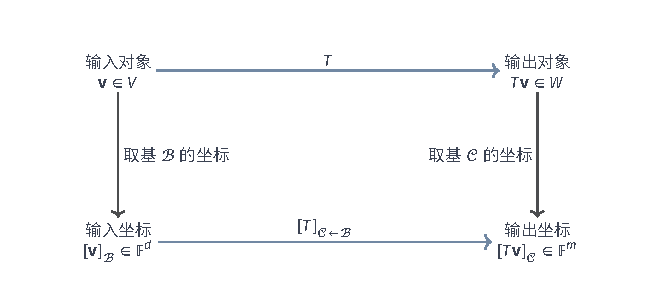
\includegraphics[width=112.0mm]{figures/01-mathematical-preliminaries-upper/02-linear-algebra-and-geometry/tikz/ch06-object-coordinate-map/figure.pdf}
  \caption{先作用于对象再取坐标，与先取输入坐标再乘矩阵，得到相同输出坐标。
 横向箭头改变对象或数值，竖向箭头只改变记录方式。}
 \label{fig:ch06-object-coordinate-map}
\end{figure}

设计矩阵$\bm X_\varepsilon$表示
$T_\varepsilon:\mathbb R^2\to\mathbb R^3$，
$\bm w\mapsto w_1\bm c_1+w_2\bm c_2$。输入是两个系数，输出是三个样本的拟合值，
不能把它们当成同一个向量。带偏置的规则$\bm x\mapsto\bm A\bm x+\bm b$在
$\bm b\neq0$时为仿射映射。增广坐标给出
\[
 \begin{bmatrix}\bm A&\bm b\\\bm0^\top&1\end{bmatrix}
 \begin{bmatrix}\bm x\\1\end{bmatrix}
 =\begin{bmatrix}\bm A\bm x+\bm b\\1\end{bmatrix}.
\]
大矩阵对增广空间是线性的，但原输入被限制在末坐标为$1$的仿射集合上，不能因此
声称原映射线性。

若两端新坐标分别满足$[\bm v]_{\mathcal B'}=\bm S_V[\bm v]_{\mathcal B}$、
$[\bm w]_{\mathcal C'}=\bm S_W[\bm w]_{\mathcal C}$，记反向坐标变换为
$\bm S_V^{-1}$，则新矩阵是$\bm S_W\bm A\bm S_V^{-1}$。
只有同一空间上的算子且两端采用同一次换基时，才成为相似关系
\begin{equation}
 \bm A_{\mathcal C}=\bm S\bm A_{\mathcal B}\bm S^{-1}.
 \label{eq:linear-algebra-similarity-change-basis}
\end{equation}
这里的逆记号表示已知可逆的坐标对应；可逆性可由下面的核与像判断。


\term{列空间}（column space）
$\operatorname{col}(\bm A)=\operatorname{range}(\bm A)
=\{\bm A\bm x:\bm x\in\mathbb F^d\}$记录可达输出；
\term{零空间}（null space）
$\operatorname{null}(\bm A)=\{\bm x:\bm A\bm x=\bm0\}$记录被消去的输入。

\term{秩}（rank）是值域维数；零度（nullity）是零空间的维数，记录被映射完全消去的独立输入方向数。
\begin{theorem}[秩零度定理]
\label{thm:linear-algebra-rank-nullity}
有限维线性映射$T:V\to W$满足
$\dim V=\dim\operatorname{null}(T)+\dim\operatorname{range}(T)$。
因此对$\bm A\in\mathbb F^{m\times d}$，
$d=\dim\operatorname{null}(\bm A)+\operatorname{rank}(\bm A)$。
\end{theorem}
\begin{proof}
取零空间的基$\bm v_1,\ldots,\bm v_r$并扩充成$V$的基
$\bm v_1,\ldots,\bm v_d$。前$r$个基向量的像为零，所以其余的像
$T\bm v_{r+1},\ldots,T\bm v_d$张成值域。若
$\sum_{j>r}a_jT\bm v_j=0$，则$\sum_{j>r}a_j\bm v_j$属于零空间，能由前$r$个
基向量表示。整个基的线性无关性迫使全部$a_j=0$，所以这些像也是无关组。
值域维数为$d-r$，结论成立。
\end{proof}


方阵$\bm A\in\mathbb F^{d\times d}$若单射，秩零度给出满射，反之亦然。
每个右端的唯一解于是定义线性逆映射，其矩阵$\bm A^{-1}$满足
$\bm A^{-1}\bm A=\bm A\bm A^{-1}=\bm I$。两个候选逆相乘可立即证明唯一性。
以下条件等价：列无关、列张成全空间、秩为$d$以及存在双侧逆。
相容乘积的逆为
$(\bm A\bm B)^{-1}=\bm B^{-1}\bm A^{-1}$。

\subsection{映射的叠加}
\label{sec:linear-algebra-map-addition}

两个预测分支接收同一个参数并输出同形预测时，可以先分别计算，再把输出加权相加。
若$T,S:V\to W$，这定义$(aT+bS)\bm x=aT\bm x+bS\bm x$；在相同的两端基下
其矩阵为$a\bm A+b\bm B$。相加的前提是两者定义域相同、取值也落在同一个空间中，
即$V$与$W$对两个映射都一致。反过来说，这个条件并不要求$V$与$W$彼此相同：
定义域与陪域是两个不同的角色，只要两个映射在同一对空间之间作用即可。

例如两个从$\mathbb R^2$到$\mathbb R^3$的映射就可以相加，它们的输入空间$\mathbb R^2$
与输出空间$\mathbb R^3$并不相同。把输入换成$T,S$定义域外的对象，或者只让其中一个
作用于$V$而另一个作用于$V'\neq V$，相加便不再有定义。
固定权重的叠加保持线性：把输入线性组合代入，各分支分别展开，再汇总即可。
若权重随输入改变，则需重新检验；例如$x\mapsto x\cdot x$由输入作为权重，已非线性。

\subsection{映射的复合}
\label{sec:linear-algebra-map-composition}

若$T:U\to V$、$S:V\to W$，复合$S\circ T$在相容基下表示为$[S][T]$。
对$\bm A\in\mathbb F^{m\times d}$、$\bm B\in\mathbb F^{d\times k}$，
矩阵计算使用式~\eqref{eq:linear-algebra-matrix-product}。
被消去的中间索引对应中间空间。先交换坐标再保留第一坐标，与先保留第一坐标再
交换，结果不同：
\[
 \begin{bmatrix}1&0\\0&0\end{bmatrix}\begin{bmatrix}0&1\\1&0\end{bmatrix}
 =\begin{bmatrix}0&1\\0&0\end{bmatrix},\qquad
 \begin{bmatrix}0&1\\1&0\end{bmatrix}\begin{bmatrix}1&0\\0&0\end{bmatrix}
 =\begin{bmatrix}0&0\\1&0\end{bmatrix}.
\]
一般不能交换因子。按中间索引展开可验证乘法结合律，因此多个相容映射的复合无需重新规定括号。

按输入和输出的分组分块，同一规则成为
$\bm C_{i,j}=\sum_\ell\bm A_{i,\ell}\bm B_{\ell,j}$，各块的尺寸仍须相容。


若中间空间的范数匹配，连续应用两次界得到次乘性
\[
 \lVert\bm A\bm B\rVert_{\alpha\to\gamma}
 \leq\lVert\bm A\rVert_{\beta\to\gamma}
       \lVert\bm B\rVert_{\alpha\to\beta}.
\]


\subsection{对象的联合运算}
\label{sec:linear-algebra-joint-operations}

在同一空间内加法与数乘产生新对象。多个数组还可以按元素、成对索引或缩并规则联合计算；先检查轴与形状，再判断固定哪些输入时运算线性。
固定一个数值掩码$\bm M$后，$\bm X\mapsto\bm M\odot\bm X$也是数组空间上的
线性映射，其中\term{逐元素乘积}（Hadamard product）满足
$(\bm M\odot\bm X)_{i,j}=m_{i,j}x_{i,j}$，不对索引求和。
例如
\[
 \begin{bmatrix}1&2\\3&4\end{bmatrix}
 \odot\begin{bmatrix}0&1\\1&0\end{bmatrix}
 =\begin{bmatrix}0&2\\3&0\end{bmatrix},
\]
相同两矩阵的普通乘积却是
$\left[\begin{smallmatrix}2&1\\4&3\end{smallmatrix}\right]$。
掩码依赖所选坐标；若两个因子都作为未知量，乘积是分别线性而非联合线性，
因为同时将两者放大两倍会把结果放大四倍。


缩并须先指定参与求和的轴，并保证对应尺寸相容。\term{张量缩并}
（tensor contraction）将指定索引对齐相乘再求和。例如
$\bm A\in\mathbb R^{m\times d\times r}$、
$\bm B\in\mathbb R^{d\times n\times r}$可定义
$c_{i,j}=\sum_{k=1}^d\sum_{s=1}^r a_{i,k,s}b_{k,j,s}$。
对$\bm X\in\mathbb R^{b\times\ell\times d}$的最后一轴应用同一矩阵
$\bm W\in\mathbb R^{d\times h}$，则
$z_{i,j,r}=\sum_k x_{i,j,k}w_{k,r}$，输出形状为$b\times\ell\times h$。
写出索引能检查哪些轴被消去、哪些轴应当保留。


加权读取给出一个实际的索引检查。设位置数$\ell$、查询与键的特征维数$d_k$、值的特征维数$d_v$均为正整数，查询、键和值分别为
$\bm Q,\bm K\in\mathbb R^{\ell\times d_k}$、
$\bm V\in\mathbb R^{\ell\times d_v}$。查询描述要匹配的特征，键用于打分，值是
实际读取的内容。\term{注意力}（attention）的一种计算为
\begin{align}
 \bm S&=\frac{\bm Q\bm K^\top}{\sqrt{d_k}}\in\mathbb R^{\ell\times\ell},
 \label{eq:linear-algebra-attention-scores}\\
 a_{i,j}&=\frac{\exp(s_{i,j})}{\sum_{r=1}^{\ell}\exp(s_{i,r})},
 \qquad\bm O=\bm A\bm V\in\mathbb R^{\ell\times d_v}.
 \label{eq:linear-algebra-attention-contraction}
\end{align}
第一次缩并消去特征轴，第二次消去被读取的位置轴。非负且每行和为$1$说明这是
加权平均；概率解释还需另有随机对象。固定$\bm A$时对$\bm V$线性，
但$\bm Q,\bm K,\bm V$通常依赖同一输入，完整注意力并不因此线性。

查询数也不必等于键数。例如
\[
 \bm Q=\begin{bmatrix}1&0\\0&1\end{bmatrix},\quad
 \bm K=\begin{bmatrix}1&0\\0&1\\1&1\end{bmatrix},\quad
 \bm V=(v_1,v_2,v_3)^\top.
\]
两个查询与三个键的配对给出
\[
 \bm Q\bm K^\top=\begin{bmatrix}1&0&1\\0&1&1\end{bmatrix}.
\]
权重形状为$2\times3$，输出为$2\times1$；需要匹配的是特征轴，不是位置数。
再取$\bm Q=\bm K=\bm I_2$和
$\bm V=\left[\begin{smallmatrix}1&1\\1&1+\varepsilon\end{smallmatrix}\right]$，
记$c=\exp(1/\sqrt2)$，则
\[
 \bm A=\frac1{c+1}\begin{bmatrix}c&1\\1&c\end{bmatrix},\qquad
 \bm O=\begin{bmatrix}
 1&1+\varepsilon/(c+1)\\1&1+c\varepsilon/(c+1)
 \end{bmatrix}.
\]
两列之差为$\varepsilon(1,c)^\top/(c+1)$，仍是$O(|\varepsilon|)$；
另一方面每个输出行是$\bm V$各行的加权平均，属于它们的张成空间。
列差与行组合检查的是两个不同的轴。

\term{卷积}（convolution）则读取局部位置并复用固定核。对窗口
$\bm U\in\mathbb R^{k_h\times k_w\times c_{\mathrm{in}}}$和核
$\bm K\in\mathbb R^{k_h\times k_w\times c_{\mathrm{in}}\times c_{\mathrm{out}}}$，
忽略偏置时
\begin{equation}
 z_r=\sum_{a=1}^{k_h}\sum_{b=1}^{k_w}\sum_{s=1}^{c_{\mathrm{in}}}
 u_{a,b,s}k_{a,b,s,r}.
 \label{eq:linear-algebra-convolution-window-contraction}
\end{equation}
固定核后它对窗口线性；窗口移动时复用核，但边界、步幅及核是否翻转必须另外规定。
此处的同向索引写法是模型中常称为卷积的互相关形式。取一维双通道窗口
$\bm U=\left[\begin{smallmatrix}1&1\\1&1+\varepsilon\end{smallmatrix}\right]$，
两个位置均以$1/2$读取第一通道的核输出$1$；核
$\bm K_2=\left[\begin{smallmatrix}0&-1\\0&1\end{smallmatrix}\right]$输出
$\varepsilon$。前者保留共同水平，后者提取局部差异。索引规则说明计算了什么，
不替代模型是否适用的判断。

两组轴分别作用时，\term{Kronecker积}（Kronecker product）记录成对索引：
\begin{equation}
 \bm A\otimes\bm B
 =\begin{bmatrix}
 a_{1,1}\bm B&\cdots&a_{1,n}\bm B\\
 \vdots&\ddots&\vdots\\
 a_{m,1}\bm B&\cdots&a_{m,n}\bm B
 \end{bmatrix}\in\mathbb F^{mp\times nq},
 \quad
 \bm A\in\mathbb F^{m\times n},\ \bm B\in\mathbb F^{p\times q}.
 \label{eq:linear-algebra-kronecker-product}
\end{equation}
按成对索引分别求和可得相容乘积的混合规则
\begin{equation}
 (\bm A\otimes\bm B)(\bm C\otimes\bm D)
 =(\bm A\bm C)\otimes(\bm B\bm D).
 \label{eq:matrix-analysis-kronecker-mixed-product}
\end{equation}
对$\bm A\in\mathbb F^{p\times m}$、$\bm X\in\mathbb F^{m\times n}$、
$\bm B\in\mathbb F^{n\times q}$，按列向量化给出
\begin{equation}
 \operatorname{vec}(\bm A\bm X\bm B)
 =(\bm B^\top\otimes\bm A)\operatorname{vec}(\bm X).
 \label{eq:matrix-analysis-vec-kronecker}
\end{equation}
证明只需看输出索引$i+(j-1)p$：两侧该元素均为
$\sum_{\ell=1}^m\sum_{k=1}^n a_{i,\ell}x_{\ell,k}b_{k,j}$。
这里是普通转置而非共轭转置，即使在复数域中也如此，因为元素乘法没有共轭。
固定$\bm A,\bm B$后这是关于$\bm X$的线性映射，不是关于全部因子的联合线性映射。
实际执行左右乘法往往比构造巨大的Kronecker矩阵省存储。

\begin{table*}[htbp]
 \centering\small
 \begin{tabularx}{\linewidth}{@{}lXX@{}}
 \toprule
 运算 & 形状条件与输出 & 索引作用\\
 \midrule
 $\bm A\bm B$ & $(m\times n)(n\times p)\to m\times p$ & 汇总共同索引\\
 $\bm A\odot\bm B$ & 同为$m\times n$，输出仍为$m\times n$ & 同位置相乘，不求和\\
 $\bm A\otimes\bm B$ & $(m\times n)$与$(p\times q)\to(mp)\times(nq)$ & 保留两组成对索引\\
 $\bm x^*\bm y$ & 两个$n$维向量，输出标量 & 共轭配对后汇总\\
 \bottomrule
 \end{tabularx}
 \caption{相乘符号对应不同操作。先检查消去哪些索引，再判断其线性性和输出含义。}
 \label{tab:linear-algebra-products-and-shapes}
\end{table*}

\subsection{对象的分解与投影}
\label{sec:linear-algebra-decomposition-projection}
\label{sec:linear-algebra-length-angle-distance}

代数直和只保证分量唯一。若要删去一个方向后让剩余误差最小，还必须规定长度与正交关系。
为什么仅“直和”还不够？直和只说清了一个向量能被唯一地拆成两部分，但并没有规定怎么拆
才能让被丢掉的那部分误差最小——在斜坐标系里沿坐标轴拆，得到的两个分量并不互相垂直，
丢掉一个后剩下的也不是最近点。只有先规定“垂直”，最近分解才唯一。
例如把向量分成沿一条直线的分量与垂直分量，垂直性取决于所用内积。
下面先定义这个配对运算，再从它推导正交分解与最近点计算。
\begin{definition}[实与复内积]
\label{def:linear-algebra-inner-product}
\label{def:functional-inner-product-space}
\term{内积}（inner product）$\langle x,y\rangle$对第二变量线性、对第一变量共轭线性，
满足$\langle y,x\rangle=\overline{\langle x,y\rangle}$，且
$\langle x,x\rangle>0$对非零$x$成立。实数域中共轭不改变数值，因此它是对称双线性配对。
配备该运算的向量空间称为\term{内积空间}（inner product space）；
长度和正交关系由配对计算得到。
\end{definition}
标准实坐标的内积是$\langle\bm x,\bm y\rangle=\bm x^\top\bm y$，
标准复坐标的内积是$\langle\bm x,\bm y\rangle=\bm x^*\bm y$。
这里$\bm A^*=\overline{\bm A}^{\top}$为共轭转置，实数情形退化为转置。
两者都满足上述配对条件，并以同一个规则诱导长度：
\begin{equation}
 \lVert\bm x\rVert=\sqrt{\langle\bm x,\bm x\rangle}.
 \label{eq:linear-algebra-inner-product-norm}
\end{equation}
零配对表示\term{正交}（orthogonal）。下面验证内积怎样控制长度与夹角。

\begin{theorem}[Cauchy--Schwarz不等式]
\label{thm:linear-algebra-cauchy-schwarz}
在实或复内积空间中，
$|\langle\bm x,\bm y\rangle|\leq\lVert\bm x\rVert\lVert\bm y\rVert$。
等号成立当且仅当两向量线性相关。
\end{theorem}
\begin{proof}
$\bm y=\bm0$时直接成立。否则令
$a=\langle\bm y,\bm x\rangle/\lVert\bm y\rVert^2$，则
\[
 0\leq\lVert\bm x-a\bm y\rVert^2
 =\lVert\bm x\rVert^2-
   \frac{|\langle\bm x,\bm y\rangle|^2}{\lVert\bm y\rVert^2}.
\]
移项即得不等式；等号恰好要求$\bm x=a\bm y$。
\end{proof}

实空间中非零向量的夹角由
$\cos\theta=\langle\bm x,\bm y\rangle/(\lVert\bm x\rVert\lVert\bm y\rVert)$定义；
复内积可能非实，不能直接沿用这一实夹角公式。在贯穿例中
$\bm c_1^\top\bm q=0$、$\lVert\bm c_1\rVert_2^2=3$、
$\lVert\bm c_2\rVert_2^2=3+2\varepsilon^2$，因此
\begin{equation}
 \cos\theta_\varepsilon=\frac{\sqrt3}{\sqrt{3+2\varepsilon^2}}\longrightarrow1.
 \label{eq:linear-algebra-nearly-collinear-angle}
\end{equation}
这给“几乎同向”一个确定的欧氏度量；更换内积也会更换角度。


一般范数不一定由内积诱导。在实向量空间中，一个范数来自内积，当且仅当它满足
\term{平行四边形恒等式}（parallelogram identity）
\begin{equation}
  \lVert f+g\rVert^2+\lVert f-g\rVert^2
  =
  2\lVert f\rVert^2+2\lVert g\rVert^2.
  \label{eq:functional-parallelogram-identity}
\end{equation}
例如在$\mathbb{R}^2$的$\ell^1$范数中取
$\bm{u}=(1,0)^{\top}$、$\bm{v}=(0,1)^{\top}$，左侧为$8$，右侧为$4$，所以这个
范数不可能来自内积。内积展开直接证明了恒等式的必要性。实数域中的反向判定可用极化公式
$B(f,g)=(\lVert f+g\rVert^2-\lVert f-g\rVert^2)/4$恢复内积：
平行四边形恒等式给出
$B(f+h,g)+B(f-h,g)=2B(f,g)$。
取$h=f$可得$B(2f,g)=2B(f,g)$，再令$f=(u+v)/2$、$h=(u-v)/2$，
便得$B(u+v,g)=B(u,g)+B(v,g)$。加法性先给出有理数齐次性，
范数的连续性再把它推广到实数齐次性。结合对称性与$B(f,f)=\lVert f\rVert^2$，
就得到所需的对称双线性正定内积。
这里完成的是实数域的反向判定；复数域需要用复极化公式恢复共轭线性，本段不展开。
能否由内积定义正交，与柯西列是否在空间内有极限，是两个不同问题；
后一个问题将在第~\ref{sec:linear-algebra-sequence-convergence}节核对。


权重可以进一步区分不同方向的代价。复方阵$\bm M$满足$\bm M^*=\bm M$时称为
Hermitian矩阵，即等于自己的共轭转置；若还对每个非零$\bm x$满足
$\bm x^*\bm M\bm x>0$，则称为Hermitian正定矩阵。这是实对称正定条件的复数对应。
这样的$\bm M$给出
$\langle\bm x,\bm y\rangle_{\bm M}=\bm x^*\bm M\bm y$和
$\lVert\bm x\rVert_{\bm M}=\sqrt{\bm x^*\bm M\bm x}$。
若$\bm M$仅半正定，配对只给半内积，诱导半范数以及
\begin{equation}
 d_{\bm M}(\bm x,\bm y)
 =\sqrt{(\bm x-\bm y)^*\bm M(\bm x-\bm y)}.
 \label{eq:linear-algebra-mahalanobis-pseudodistance}
\end{equation}
半正定的Cauchy--Schwarz仍可从
$\langle\bm x+t\bm y,\bm x+t\bm y\rangle_{\bm M}\geq0$得到，因而三角不等式
保留；不同点的距离却可能为零。这是定义~\ref{def:analysis-pseudometric}的伪距离。
例如$\bm M=\operatorname{diag}(1,0)$无法区分$(0,0)^\top$和$(0,1)^\top$。
后文构造$\bm M=\bm L^*\bm L$后，还能把它写成
$\lVert\bm L(\bm x-\bm y)\rVert_2$：正定时只是改变几何，退化时则消去方向。

对同形矩阵，把元素视为有限坐标，得到Frobenius内积
$\langle\bm A,\bm B\rangle_{\mathrm F}=\sum_{i,j}\overline{a_{i,j}}b_{i,j}$，
以及$\lVert\bm A\rVert_{\mathrm F}=(\sum_{i,j}|a_{i,j}|^2)^{1/2}$。
这是矩阵作为对象的长度；它与矩阵作为变换时的最大放大率并非同一口径。


有限维的分解可以直接构造。设$U$是有限维内积空间的子空间，
$U^\perp=\{r:\langle u,r\rangle=0,\ u\in U\}$为正交补。
对$U$的一组基逐次计算
\[
 v_j=b_j-\sum_{i<j}q_i\langle q_i,b_j\rangle,\qquad q_j=v_j/\lVert v_j\rVert.
\]
若$v_j=0$，原向量已由此前方向张成，与基的无关性矛盾；因此每次归一化合法。
这就是Gram--Schmidt正交化，它给出$U$的正交归一基。
对任意$y$，取$p=\sum_j q_j\langle q_j,y\rangle$，则$r=y-p$与每个$q_j$正交，
所以$y=p+r\in U+U^\perp$。两种分解之差属于$U\cap U^\perp=\{0\}$，故唯一。
又对任意$u\in U$，
$\lVert y-u\rVert^2=\lVert r\rVert^2+\lVert p-u\rVert^2$，最近点唯一为$p$。
这个证明只用有限基与内积，不调用无限维投影定理。
把上述最近分量记为$\widehat{\bm y}$，映射$\bm y\mapsto\widehat{\bm y}$称为
\term{正交投影}（orthogonal projection）\scite{math-axler2015linear}。
若$\bm Q$的列为$U$的标准正交基，
$\bm Q^*\bm Q=\bm I$，系数直接由内积读取：
\begin{equation}
 \widehat{\bm y}=\bm Q\bm Q^*\bm y,\qquad
 \bm P_U=\bm Q\bm Q^*,\quad \bm P_U^*=\bm P_U,\quad\bm P_U^2=\bm P_U.
 \label{eq:linear-algebra-orthogonal-projector}
\end{equation}

一般基不能直接用内积读出坐标，因为基向量之间还会互相贡献。
\begin{definition}[有限向量族的Gram矩阵]
\label{def:linear-algebra-gram-matrix}
向量$\bm b_1,\ldots,\bm b_r$的\term{Gram矩阵}（Gram matrix）为
$g_{i,j}=\langle\bm b_i,\bm b_j\rangle$。若$\bm B$以它们为列，标准坐标中
$\bm G=\bm B^*\bm B$，加权坐标中$\bm G=\bm B^*\bm M\bm B$。
\end{definition}
因为$\bm a^*\bm G\bm a=\lVert\sum_j a_j\bm b_j\rVert^2$，Gram矩阵半正定，
且在内积正定时，正定当且仅当这组向量线性无关。令
$\widehat{\bm y}=\sum_j a_j\bm b_j$，残差与每个$\bm b_i$正交要求
\[
 \sum_j g_{i,j}a_j=\langle\bm b_i,\bm y\rangle.
\]
这给出投影系数的线性方程，而非一组可直接独立读取的坐标。怎样解它，以及方向
冗余时怎样选择系数，留给第~\ref{sec:linear-algebra-reachability-solvability}节。

\begin{example}[同一子空间的两种最近点]
\label{ex:linear-algebra-weighted-projection}
在$\mathbb R^2$中取
\[
 \bm b=(2,1)^\top,\qquad U=\operatorname{span}\{(1,1)^\top\}.
\]
欧氏投影的标量系数满足$2a=3$，故$\bm p=(1.5,1.5)^\top$。
改用$\bm M=\operatorname{diag}(1,4)$，系数满足$5a=6$，得到
$\bm p_{\bm M}=(1.2,1.2)^\top$。第二坐标误差代价更大，最近点便向$b_2=1$靠近。
残差$(0.8,-0.2)^\top$与$(1,1)^\top$的普通内积非零，加权内积却为零。
\end{example}
\begin{figure*}[htbp]
  \centering
  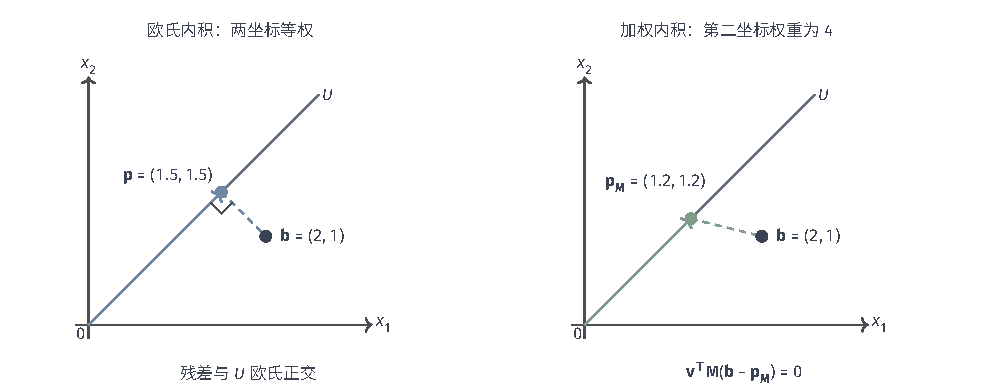
\includegraphics[width=168.998mm]{figures/01-mathematical-preliminaries-upper/02-linear-algebra-and-geometry/tikz/linear-algebra-weighted-projection/figure.pdf}
  \caption{同一目标在同一直线上的欧氏投影与加权投影。实箭头是投影向量，虚线是残差；
 右图画在普通坐标中，残差不必形成欧氏直角。正交性必须用所选内积判断。}
 \label{fig:linear-algebra-weighted-projection}
\end{figure*}


换基时，保持同一抽象几何需同时变换范数。若新坐标$\bm z=\bm S\bm x$，
原长度应写成$\lVert\bm S^{-1}\bm z\rVert$。把新坐标直接按普通欧氏长度比较，
一般已经换了问题。复方阵$\bm U$满足$\bm U^*\bm U=\bm I$时，称为酉矩阵（unitary matrix）。
它保持长度，因为
\[
 \lVert\bm U\bm x\rVert_2^2
 =\bm x^*\bm U^*\bm U\bm x
 =\lVert\bm x\rVert_2^2.
\]
实数情形就是正交矩阵。因此两端正交或酉换基保持欧氏几何，而一般换基不保持。
这也是前面的大坐标不能单独解释为大对象的原因。

\subsection{对象的标量读取}
\label{sec:linear-algebra-scalar-readouts}

从一组样本中读取加权总和，或从一个向量中读取某个坐标，输出都是一个标量。
这样的读取先要确定规则及其误差放大率。把矩阵本身作为输入时，还需区分迹这样的
线性读取与行列式这样的非线性标量量；把读取接在映射后面时，则要找出输入端的等效读取。
保持线性组合的标量读取称为\term{线性泛函}（linear functional）：
它是映射$\ell:V\to\mathbb F$，满足$\ell(ax+by)=a\ell(x)+b\ell(y)$。
固定有限维正交归一基$(q_j)$，令
$h=\sum_j\overline{\ell(q_j)}q_j$。若$x=\sum_j x_jq_j$，则
$\langle h,x\rangle=\sum_j\ell(q_j)x_j=\ell(x)$。
因此每次线性读取对应唯一方向$h$；两种表示之差与自身配对即可证明唯一性。
Cauchy--Schwarz给出$|\ell(x)|\leq\lVert h\rVert\lVert x\rVert$，
当$h\neq0$时，在$h/\lVert h\rVert$上取到等号；$h=0$时读取恒为零。这是有限维内积表示，不依赖后面的Riesz定理。
若关心的是一次线性读取$\bm z^*\bm r$，最坏误差还取决于读取方向$\bm z$。
\begin{definition}[有限维对偶范数]
\label{def:linear-algebra-dual-norm}
给定$\mathbb F^d$上的范数，相对于标准坐标配对的\term{对偶范数}（dual norm）为
\begin{equation}
 \lVert\bm z\rVert_*=\sup_{\lVert\bm r\rVert\leq1}|\bm z^*\bm r|.
 \label{eq:linear-algebra-dual-norm-definition}
\end{equation}
\end{definition}
此处先按上确界定义；常用坐标范数下的有限性与取到上界可直接验证。它满足范数公理，因为线性读取
满足三角不等式和齐次性，且非零$\bm z$总能读取某个坐标得到非零值。
Hölder给出$\ell_p$单位球上的上界$\lVert\bm z\rVert_q$。若$\bm z=0$，所有读取值均为零，
取$\bm r=0$即可达到上界。以下对$\bm z\neq0$核对达到性。当$1<p<\infty$时，取
\[
 r_j=\frac{z_j}{|z_j|}
       \frac{|z_j|^{q-1}}{\lVert\bm z\rVert_q^{q-1}}\quad(z_j\neq0),
 \qquad r_j=0\quad(z_j=0),
\]
就有$\lVert\bm r\rVert_p=1$且$\bm z^*\bm r=\lVert\bm z\rVert_q$。
$p=1$时把单位预算放在$|z_j|$最大的坐标，让该$r_j$与对应的$z_j$同相；
$p=\infty$时，对每个$z_j\neq0$取$r_j=z_j/|z_j|$，使
$\overline{z_j}r_j=|z_j|$；$z_j=0$时可取$r_j=0$。这里匹配的是每一对对应坐标的相位。
因而
\begin{equation}
 (\lVert\cdot\rVert_p)_*=\lVert\cdot\rVert_q,\qquad \frac1p+\frac1q=1,
 \label{eq:linear-algebra-lp-duality}
\end{equation}
并对$\rho\geq0$有
\begin{equation}
 \max_{\lVert\bm r\rVert_p\leq\rho}|\bm z^*\bm r|
 =\rho\lVert\bm z\rVert_q.
 \label{eq:linear-algebra-linear-perturbation-duality}
\end{equation}
例如$\bm z=(2,-1)^\top$、$|r_j|\leq0.01$时最大变化为$0.03$，
由$\bm r=(0.01,-0.01)^\top$达到。图~\ref{fig:linear-algebra-dual-unit-balls}
固定同一次读取，显示预算形状怎样改变最坏方向。非线性函数若只用此界控制一阶项，
还必须另控余项；这里的对偶范数也不同于第~\ref{sec:opt-duality}节从约束问题构造
下界的拉格朗日对偶。

\begin{figure*}[htbp]
  \centering
  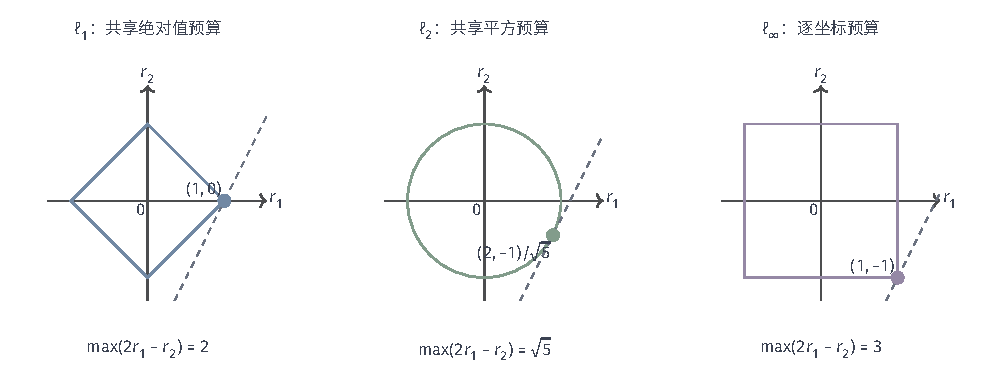
\includegraphics[width=168.998mm]{figures/01-mathematical-preliminaries-upper/02-linear-algebra-and-geometry/tikz/linear-algebra-dual-unit-balls/figure.pdf}
  \caption{同一线性读取$2r_1-r_2$在$\ell_1$、$\ell_2$、$\ell_\infty$单位球上的
 最大值依次为$2$、$\sqrt5$、$3$。虚线为最后接触可行集的支撑直线，点为最大化方向。
 三图坐标尺度相同，均为解析教学例；改变允许误差的形状会改变误差常数。}
 \label{fig:linear-algebra-dual-unit-balls}
\end{figure*}
\FloatBarrier


下面转向两个直接从矩阵读出数值的量。它们都不经过任何输入方向，却分别回答两个
常见问题：一批作用的总量是多少，以及作用有没有把空间压扁。
方阵的\term{迹}（trace）为$\operatorname{tr}\bm A=\sum_i a_{i,i}$，
是将两个索引对齐后求和，因此给出对角方向上各作用的合计。
对$\bm A\in\mathbb F^{m\times n}$、
$\bm B\in\mathbb F^{n\times m}$，
\begin{equation}
 \operatorname{tr}(\bm A\bm B)=\sum_{i,j}a_{i,j}b_{j,i}
 =\operatorname{tr}(\bm B\bm A).
 \label{eq:linear-algebra-trace-cyclic}
\end{equation}
更多因子只能合法循环移动，一般不能任意换序。因此
$\operatorname{tr}(\bm A\bm B\bm C)=\operatorname{tr}(\bm B\bm C\bm A)$，
但不保证等于$\operatorname{tr}(\bm A\bm C\bm B)$。相似变换不改变迹。
Frobenius内积也可写成$\operatorname{tr}(\bm A^*\bm B)$。


迹是对整个矩阵线性的标量读取；方阵的体积缩放则由另一种标量量描述。
\term{行列式}（determinant）由对每列线性、
交换两列变号和$\det\bm I=1$刻画；实数域中$\det\bm A$给出有向体积缩放，
绝对值为体积比，符号表示定向。列相关时平行多面体被压低维，行列式为零。
例如取$\bm X_\varepsilon$前两行得到
$\bm A_\varepsilon=\left[\begin{smallmatrix}1&1\\1&1+\varepsilon\end{smallmatrix}\right]$，
则$\det\bm A_\varepsilon=\varepsilon$。复合满足
$\det(\bm A\bm B)=\det\bm A\det\bm B$。行列式检测体积退化，却随整体尺度和维数
变化，不能独自衡量某个方向的误差放大。


列相关使行列式为零；列无关则可经有限次可逆列变换化到单位矩阵，
各步只乘以非零尺度或改变符号，故行列式非零。
所以方阵可逆恰好等价于行列式非零，可逆时$\det(\bm A^{-1})=1/\det\bm A$。
迹是矩阵空间上的线性读取，行列式则对每列分别线性，通常不是对整个矩阵线性。

现在回到向量的线性读取。若先计算$T x$，再沿输出方向$y$读取
$\langle y,Tx\rangle_W$，能否直接在输入端读取$x$，得到同一个数？
下面的伴随为每个输出读取方向$y$找出这样的输入方向；它不要求从输出恢复全部输入。
\begin{definition}[有限维伴随]
\label{def:linear-algebra-adjoint}
对内积空间之间的线性映射$T:V\to W$，伴随$T^*:W\to V$满足
$\langle Tx,y\rangle_W=\langle x,T^*y\rangle_V$。
它把输出端读取转移到输入端。
\end{definition}
对固定$y$，线性读取$x\mapsto\langle y,Tx\rangle_W$由唯一方向$T^*y$表示，
取共轭便得上述等式。将$ay_1+by_2$代入配对式并展开，再用表示方向的唯一性，便有
$T^*(ay_1+by_2)=aT^*y_1+bT^*y_2$，所以$T^*$是线性映射。
上述伴随把输出端的线性配对搬回输入端：
\[
 \langle T\bm x,\bm y\rangle_W=\langle\bm x,T^*\bm y\rangle_V.
\]
标准正交坐标下，
$\langle\bm A\bm x,\bm y\rangle=\bm x^*\bm A^*\bm y$，所以伴随矩阵就是
\term{共轭转置}（conjugate transpose）$\bm A^*$，实数时是
\term{转置}（transpose）$\bm A^\top$。逐元素有
$(\bm A^\top)_{i,j}=a_{j,i}$；复数时不能省略共轭，否则平方长度可能不是非负实数。
若输入、输出内积由正定$\bm M_V,\bm M_W$表示，伴随矩阵$\bm B$应满足
\[
 \bm x^*\bm A^*\bm M_W\bm y=\bm x^*\bm M_V\bm B\bm y,
 \qquad\text{即}\qquad \bm M_V\bm B=\bm A^*\bm M_W.
\]
两端权重可逆，因而可以求出$\bm B$的显式形式。伴随完成的是配对转移，不是一般意义的逆：
例如$\bm A=2\bm I$的伴随仍为$2\bm I$，反向恢复输入却应除以$2$。


两端权重矩阵正定、因而可逆，给出加权伴随：
$\bm A^\sharp=\bm M_V^{-1}\bm A^*\bm M_W$，其中两端权重均正定。
例如$\bm A=\left[\begin{smallmatrix}0&1\\0&0\end{smallmatrix}\right]$、
$\bm M_V=\bm M_W=\operatorname{diag}(1,4)$时，
$\bm A^\sharp=\left[\begin{smallmatrix}0&0\\1/4&0\end{smallmatrix}\right]$，
而普通转置的对应元素为$1$。伴随随几何改变，仍不等于逆。


将行约束在标准输入内积中表示为向量，得到\term{行空间}（row space）
$\operatorname{range}(\bm A^*)\subseteq\mathbb F^d$；
实数时就是各行转为列后的张成空间，复数时还需共轭。
左零空间$\operatorname{null}(\bm A^*)\subseteq\mathbb F^m$则记录无法读取到任何
列空间分量的输出方向。由配对等式，
\[
 \operatorname{null}(\bm A)=\operatorname{range}(\bm A^*)^\perp,\qquad
 \operatorname{null}(\bm A^*)=\operatorname{range}(\bm A)^\perp.
\]
例如$\bm x$与$\bm A^*\bm y$对所有$\bm y$正交，当且仅当
$\bm y^*\bm A\bm x=0$对所有$\bm y$成立，也就是$\bm A\bm x=0$。
这同时解释了四个子空间分属输入端与输出端。


再由正交补关系，
$\operatorname{rank}(\bm A^*)=d-\dim\operatorname{null}(\bm A)
=\operatorname{rank}(\bm A)$，证明行秩与列秩相等。令$r=\operatorname{rank}(\bm A)$，
输入端的行空间$\operatorname{range}(\bm A^*)$与零空间$\operatorname{null}(\bm A)$
维数分别为$r$与$d-r$；输出端的列空间$\operatorname{range}(\bm A)$与
左零空间$\operatorname{null}(\bm A^*)$维数分别为$r$与$m-r$。


复合作用的读取还验证$(\bm A\bm B)^*=\bm B^*\bm A^*$：
配对先经过$\bm A$再经过$\bm B$的伴随，次序反向。
伴随还使左右两侧的作用界能够互相转换。要控制矩阵乘积的总平方大小，
可以先逐列估计左乘的放大，再通过共轭转置把右乘化为同一问题。
逐列应用诱导范数界，再对伴随应用同样结论，得到
\begin{equation}
 \lVert\bm A\bm B\rVert_{\mathrm F}
 \leq\lVert\bm A\rVert_2\lVert\bm B\rVert_{\mathrm F},
 \qquad
 \lVert\bm A\bm B\rVert_{\mathrm F}
 \leq\lVert\bm A\rVert_{\mathrm F}\lVert\bm B\rVert_2.
 \label{eq:matrix-analysis-mixed-submultiplicativity}
\end{equation}
其中$\lVert\bm B^*\rVert_2=\lVert\bm B\rVert_2$可由
$\lVert\bm B\rVert_2=\max_{\lVert\bm x\rVert_2=\lVert\bm y\rVert_2=1}
|\bm y^*\bm B\bm x|$交换两向量得到，不需预先使用SVD。
又因$\lVert\bm A\rVert_2\leq\lVert\bm A\rVert_{\mathrm F}$，
Frobenius范数也次乘。

\subsection{方阵的幂、指数和平方根}
\label{sec:matrix-analysis-functions-structured-operations}
\label{sec:ch06-powers-spectrum}
\label{sec:matrix-analysis-spectrum}
\label{sec:ch06-triangular-spectrum}

固定一个方阵$\bm A$以后，可以反复复合它，并叠加不同次数的作用。
这定义矩阵多项式$p(\bm A)=\sum_{j=0}^k a_j\bm A^j$，其中$\bm A^0=\bm I$。
矩形矩阵一般不能同自身复合，故此处要求方阵。与逐元素函数也要区分：
若$\bm N=\left[\begin{smallmatrix}0&1\\0&0\end{smallmatrix}\right]$，则
$\bm N^2=\bm0$，矩阵指数为$\bm I+\bm N$，并不是将四个元素分别取指数所得的数表。

标量幂级数$f(z)=\sum_{j=0}^{\infty}a_jz^j$在收敛半径$R$内绝对收敛。
先采用行和诱导范数，若$\lVert\bm A\rVert<R$，则
\[
 \sum_{j=0}^\infty\lVert a_j\bm A^j\rVert
 \leq\sum_{j=0}^\infty|a_j|\lVert\bm A\rVert^j<\infty.
\]
每个矩阵坐标的绝对值不超过行和范数；标量绝对收敛保证各坐标都有极限，有限行列数又使坐标极限给出矩阵极限，从而定义$f(\bm A)$。这是便于检验的充分条件，
不是必要条件；下面建立谱表示后，将以谱半径给出更细结论。
特别地，
\begin{equation}
 \exp(\bm A)=e^{\bm A}=\sum_{j=0}^{\infty}\frac{\bm A^j}{j!}
 \label{eq:matrix-analysis-matrix-exponential}
\end{equation}
对任意有限方阵都收敛，且$\lVert e^{\bm A}\rVert\leq e^{\lVert\bm A\rVert}$。
用前$k+1$项计算时，尾项范数不超过
$e^{\lVert\bm A\rVert}\lVert\bm A\rVert^{k+1}/(k+1)!$。
这控制截断误差，尚不评价浮点求和的误差。

标量恒等式不能忽略非交换性。按$t$展开，
\[
 e^{t\bm A}e^{t\bm B}-e^{t(\bm A+\bm B)}
 =\frac{t^2}{2}(\bm A\bm B-\bm B\bm A)+O(t^3).
\]
所以一般$e^{\bm A+\bm B}\neq e^{\bm A}e^{\bm B}$；
若$\bm A\bm B=\bm B\bm A$，绝对收敛允许重排级数，二项式公式才恢复这个等式。
同理$\sum_{j\geq0}\bm A^j$在$\lVert\bm A\rVert<1$时收敛，
其部分和乘$\bm I-\bm A$得到$\bm I-\bm A^{k+1}$，为后面构造逆提供依据。
平方根、对数和实数次幂则必须检查谱及定义域，不能仅凭逐元素公式定义。


求解器的一次更新只是一次变换；应用十次得到什么，与应用次数趋于无穷会怎样，
需要分别回答。前一个问题要求计算有限矩阵幂，后一个问题还要研究其中各项的极限。
为了把两者放在同一个可算例子里，本节固定
\begin{equation}
 \bm A=\begin{bmatrix}0.8&4\\0&0.5\end{bmatrix},
 \qquad
 \bm x^{(0)}=\begin{bmatrix}0\\1\end{bmatrix},
 \qquad \bm x^{(k+1)}=\bm A\bm x^{(k)}.
 \label{eq:ch06-fixed-iteration-example}
\end{equation}
这是$\mathbb R^2$到自身的方阵，与近共线设计矩阵是不同对象。第一步
$\bm x^{(1)}=(4,0.5)^\top$已比初值长得多，但这并不能判断长期是否发散。


直接相乘会不断混合坐标。若某些方向在作用后保持不变，就可以沿它们分别计算；
若找不到足够多这样的方向，则要保留方向间的三角耦合。谱表示的任务是找到这些
适合计算的坐标，并说明换坐标是否保留原来的长度。


在式~\eqref{eq:ch06-fixed-iteration-example}中，
$\bm A(1,0)^\top=0.8(1,0)^\top$：这条直线只被缩放，没有转向。
这给“反复作用一个方阵会怎样”提供了关键线索：普通向量每作用一次就和其他坐标混合，
长期行为难以直接看出；但若存在某些特殊方向，向量落在其上时经过$\bm A$作用后仍在同一
直线上（只是被整体缩放），那么沿这些方向分解任意向量后，反复作用就退化成反复乘一个
标量，长期行为立刻可以判断。特征值与特征向量正是用来标记这种“不转向、只缩放”的方向。
一般地，方阵$\bm A\in\mathbb F^{d\times d}$若满足
\begin{equation}
 \bm A\bm v=\lambda\bm v,\qquad \bm v\neq\bm0,
 \label{eq:matrix-analysis-eigenpair}
\end{equation}
就称$\lambda$为\term{特征值}（eigenvalue），$\bm v$为相应
\term{特征向量}（eigenvector）。该方向的长度每次乘以$|\lambda|$；
实负特征值还使方向反向，复特征值则包含相位变化。实矩阵的全部谱也可能需要
在$\mathbb C$中描述，例如二维$90$度旋转矩阵的特征值为$\pm\mathrm i$，
没有非零实特征向量，却保留整个实平面。

这提示应同时考虑\term{不变子空间}（invariant subspace）$S$，即
$\bm A S\subseteq S$。一维不变子空间给出特征方向，更高维不变子空间允许内部
仍有混合。固定$\lambda$的特征空间为$\ker(\bm A-\lambda\bm I)$；
它包含零向量，非零成员才称特征向量。
由可逆性判据，特征值恰是\term{特征多项式}（characteristic polynomial）
\begin{equation}
 p_{\bm A}(z)=\det(z\bm I-\bm A)
 \label{eq:matrix-analysis-characteristic-polynomial}
\end{equation}
的根。根的次数称代数重数，特征空间维数称几何重数。把该特征空间的一组基扩充成
全空间的基，矩阵成为左上块$\lambda\bm I$、左下块为零的分块上三角形式，
所以特征多项式至少含相同次数的$(z-\lambda)$：几何重数不超过代数重数。
不同特征值的特征向量线性无关，可对一个最短线性依赖式应用
$\bm A-\lambda\bm I$，消去其中一个非零项而得到矛盾。

即使特征方向不够，\term{Cayley--Hamilton定理}（Cayley--Hamilton theorem）
仍把高次幂化为有限的低次幂组合。
\begin{theorem}[Cayley--Hamilton定理]
若$p_{\bm A}(z)=z^d+c_{d-1}z^{d-1}+\cdots+c_0$，则
\[
 p_{\bm A}(\bm A)
 =\bm A^d+c_{d-1}\bm A^{d-1}+\cdots+c_0\bm I=\bm0.
\]
\end{theorem}
\begin{proof}
这里$\operatorname{adj}(\bm B)$表示代数余子式矩阵的转置，称为古典伴随，
与前面由内积定义的伴随$\bm B^*$不同。按行列式展开，
$\bm B\operatorname{adj}(\bm B)=\det(\bm B)\bm I$，所以
$(z\bm I-\bm A)\operatorname{adj}(z\bm I-\bm A)=p_{\bm A}(z)\bm I$。
各余子式至多含$d-1$个一次因子的乘积，故可将古典伴随写成
$\sum_{j=0}^{d-1}z^j\bm B_j$。比较系数，
得$\bm B_{d-1}=\bm I$、
$\bm B_{j-1}-\bm A\bm B_j=c_j\bm I$和
$-\bm A\bm B_0=c_0\bm I$。将中间各式分别左乘$\bm A^j$后相加，
相邻$\bm B_j$项抵消，得到所述等式。$d=1$时直接由首尾两项得到结论。
\end{proof}
因此所有高次幂都能化成$\bm I,\ldots,\bm A^{d-1}$的线性组合，不要求可对角化。
本节的二维矩阵满足
$\bm A^2-1.3\bm A+0.4\bm I=\bm0$，所以轨迹满足
$\bm x^{(k+2)}=1.3\bm x^{(k+1)}-0.4\bm x^{(k)}$。
这类有限幂关系也能判断线性输入所生成的可达方向何时停止增加，轨迹控制中的应用可参考
\BookChapterRef{chap:control-theory}{卷2《数学准备：概率、因果与决策》第5章“策略的实现与轨迹控制”}。


特征方向不够成基时，仍能逐步选取相互正交的坐标，把混合作用限制在上三角部分。
\begin{theorem}[复Schur分解]
任意$\bm A\in\mathbb C^{d\times d}$均存在酉矩阵$\bm Q$和上三角矩阵$\bm T$，使
\begin{equation}
 \bm A=\bm Q\bm T\bm Q^*,\qquad \bm Q^*\bm Q=\bm I.
 \label{eq:matrix-analysis-schur-decomposition}
\end{equation}
$\bm T$的对角元为$\bm A$的特征值，计入代数重数。
\end{theorem}
\begin{proof}
复特征多项式有根，取相应单位特征向量$\bm q_1$并扩充为酉基$\bm Q_1$。
于是$\bm Q_1^*\bm A\bm Q_1=
\left[\begin{smallmatrix}\lambda_1&\bm a^*\\0&\bm B\end{smallmatrix}\right]$。
对$\bm B$按维数归纳作酉三角化，与第一坐标合并即得$\bm T$。
三角行列式是对角元乘积，故其特征值正是对角元。
\end{proof}

实矩阵也有$\bm A=\bm Q\bm T\bm Q^\top$的实Schur形式，其中$\bm Q$正交，
$\bm T$为分块上三角矩阵，对角块大小为$1$或$2$。非实共轭特征值对应一个实二维
不变子空间，故要由$2\times2$块一起表示。这里的Schur分解是保持内积的换基，
定义~\ref{def:matrix-analysis-schur-complement}中的Schur补则是消元后剩余的系数块；
同一个名字不意味着同一种操作。

若有$d$个线性无关特征向量，将其排成$\bm V$，就进一步得到
\[
 \bm A=\bm V\bm\Lambda\bm V^{-1}.
\]
这称为\term{对角化}（diagonalization）。在复数域中，它等价于每个特征值的
几何重数等于代数重数。一般相似关系只保持同一算子的代数结构；
酉相似还保持欧氏长度。任意对角化的$\bm V$未必酉，坐标变换可能放大误差。

若方向不足，Jordan形式用广义特征向量补齐。所谓广义特征向量，是对某个正整数$j$
满足$(\bm A-\lambda\bm I)^j\bm v=\bm0$的非零向量。
一条链从非零特征向量$\bm v_1$开始，满足
$(\bm A-\lambda\bm I)\bm v_1=\bm0$，后续向量满足
$(\bm A-\lambda\bm I)\bm v_{j+1}=\bm v_j$。也就是说，减去共同缩放后，
每个方向被送到链中前一个方向，链首被送到零。链是否足以覆盖全空间，需要下面的结构结论。
\begin{theorem}[复矩阵的Jordan链分解]
任意复方阵都有一组由上述链组成的基。在这组基下，矩阵由对角块
\[
 \bm J_s(\lambda)=\lambda\bm I+\bm N,\qquad
 N_{i,i+1}=1,\quad \bm N^s=\bm0
\]
组成，其余$N_{i,j}=0$。
\end{theorem}
\begin{proof}
先按不同特征值分开空间。特征多项式在复数域中分解为互素因子
$p_i(z)=(z-\lambda_i)^{m_i}$的乘积，Cayley--Hamilton定理说明乘积作用于$\bm A$为零。
互素的两个多项式$p,q$可由多项式辗转相除得到$up+vq=1$。
若$p(\bm A)q(\bm A)x=0$，则
$x=v(\bm A)q(\bm A)x+u(\bm A)p(\bm A)x$，两项分别属于
$\ker p(\bm A)$与$\ker q(\bm A)$；它们的交为零，因为交中向量代入同一恒等式得到$x=0$。
逐次使用这一分解，得到全空间为各$\ker p_i(\bm A)$的直和。
在每个这样的空间上，$N=\bm A-\lambda_i\bm I$满足$N^{m_i}=0$，只需再分解幂零作用。

设非零空间上的$N$满足$N^s=0$且$N^{s-1}\neq0$，取$v$使$N^{s-1}v\neq0$。
向量$v,Nv,\ldots,N^{s-1}v$线性无关：若有关系，取最小的非零系数下标$j$，
再作用$N^{s-1-j}$便得到矛盾。记其张成空间为$U$。
扩充这组向量为全空间的基，可定义线性读取$\ell$，使
$\ell(N^{s-1}v)=1$，而$\ell(N^jv)=0$对$j<s-1$成立。
令
\[
 P x=\sum_{j=0}^{s-1}\ell(N^{s-1-j}x)N^jv.
\]
代入链中各向量可得$P|_U=I$，所以$P^2=P$；利用$N^s=0$逐项移位又得$PN=NP$。
因此$\ker P$也在$N$下不变，且全空间为$U\oplus\ker P$。
在维数更小的$\ker P$上重复，便将幂零作用分成若干链。
各链逆序排列为$N^{s-1}v,\ldots,Nv,v$，恰好得到超对角元为$1$的块；
再合并不同特征值的直和，得到所需基。
\end{proof}
大小$s>1$的块把“缺少独立特征方向”记录为非零的幂零部分。
例如$\left[\begin{smallmatrix}0.8&1\\0&0.8\end{smallmatrix}\right]$
只有一个特征方向；它不能因为对角元相同就被当成$0.8\bm I$。
Jordan形式用于解释结构，数值计算通常采用Schur形式，不主动构造可能极敏感的链基。


协方差、Gram矩阵和二阶导数的对称性，使三角耦合进一步消失。
它们不仅有足够特征方向，还能使这些方向彼此正交\scite{math-horn2013matrix}。
\begin{theorem}[自伴矩阵的谱定理]
\label{thm:matrix-analysis-symmetric-spectral-theorem}
若$\bm A\in\mathbb R^{d\times d}$满足$\bm A^\top=\bm A$，则全部特征值为实数，
并存在正交矩阵$\bm Q$及实对角矩阵$\bm\Lambda$使
\begin{equation}
 \bm A=\bm Q\bm\Lambda\bm Q^\top.
 \label{eq:matrix-analysis-symmetric-eigendecomposition}
\end{equation}
复Hermitian矩阵$\bm A^*=\bm A$同样有实特征值及酉分解
$\bm A=\bm Q\bm\Lambda\bm Q^*$。
\end{theorem}
\begin{proof}
先在复数域取特征对。由
$\bm v^*\bm A\bm v=\lambda\bm v^*\bm v$，左侧为实数且$\bm v^*\bm v>0$，
知$\lambda$为实数。实对称时，把$\bm v$拆成实部和虚部，至少一个给出非零实特征向量。
若$\bm v_i,\bm v_j$对应不同特征值，则
\[
 \lambda_j\bm v_i^*\bm v_j
 =\bm v_i^*\bm A\bm v_j
 =(\bm A\bm v_i)^*\bm v_j
 =\lambda_i\bm v_i^*\bm v_j,
\]
从而彼此正交。取单位特征向量$\bm q_1$。对$\bm x\perp\bm q_1$，
$\bm q_1^*\bm A\bm x=(\bm A\bm q_1)^*\bm x=0$，
所以其正交补不变，限制后的算子仍自伴。在该正交补上按维数归纳，
得到其余标准正交特征向量，与$\bm q_1$合并即得全空间的基。
\end{proof}

若$\bm x=\sum_i c_i\bm q_i$，则
\begin{equation}
 \bm x^*\bm A\bm x=\sum_i\lambda_i|c_i|^2.
 \label{eq:matrix-analysis-quadratic-spectral-form}
\end{equation}
因此正定等价于所有特征值正，半正定等价于所有特征值非负；正、负特征方向分别
给出二次型增大和减小的方向。普通复转置对称$\bm A^\top=\bm A$不够，
例如$\bm A=\mathrm i\bm I$虽满足转置对称，特征值却非实。

更一般地，满足$\bm A^*\bm A=\bm A\bm A^*$的方阵称为正规矩阵（normal matrix）。
复数域中它恰好允许酉对角化：Schur形式仍正规，比较第一行与第一列的平方范数可知
第一行非对角元全为零，逐维归纳即得对角形式；反向由对角矩阵直接验证。
自伴矩阵属于这一类。非正规矩阵则不允许这样的正交特征表示，
即使能对角化，也可能像本节二维例那样通过非正交方向产生短时放大。

这些表示也把本小节开头的函数运算落实到谱坐标。
若$\bm A=\bm V\bm\Lambda\bm V^{-1}$，对定义在其谱上的单值函数$f$，令
\begin{equation}
 f(\bm A)=\bm V\operatorname{diag}(f(\lambda_1),\ldots,f(\lambda_d))\bm V^{-1}.
 \label{eq:matrix-analysis-matrix-function-diagonalizable}
\end{equation}
重复特征值的整个特征空间都乘以同一标量，故更换其中的基不改变结果。
多项式由相似变换的乘法直接满足该式；收敛幂级数可逐项换基，也得到相同定义。
不可对角化时，仅给根上的函数值已不够，还要有块大小所需的导数。对在谱附近解析的$f$，
\begin{equation}
 f(\bm J_s(\lambda))
 =\sum_{j=0}^{s-1}\frac{f^{(j)}(\lambda)}{j!}\bm N^j.
 \label{eq:ch06-jordan-function}
\end{equation}
这是Taylor展开在$\bm N^s=\bm0$后精确终止的结果。特别地，
\[
 e^{t\bm J}=e^{t\lambda}\sum_{j=0}^{s-1}\frac{t^j}{j!}\bm N^j.
\]
指数中的多项式因子不是数值近似误差，而是幂零耦合的真实作用。

设标量级数$\sum_{k\geq0}a_kz^k$的收敛半径为$R$，矩阵的
\term{谱半径}（spectral radius）为
$\rho(\bm A)=\max_i|\lambda_i(\bm A)|$。
若$\rho(\bm A)<R$，则矩阵级数绝对收敛。确实，取
$\rho(\bm A)<r<R$；Jordan块的二项式展开表明存在常数$C_r$使
$\lVert\bm A^k\rVert\leq C_r r^k$，因为有限次多项式增长能被较大的指数$r^k$
控制，零特征值块则在有限步后为零。于是
$\sum_k|a_k|\lVert\bm A^k\rVert\leq C_r\sum_k|a_k|r^k<\infty$。
这比$\lVert\bm A\rVert<R$的条件更弱。例如本节$\bm A$的欧氏诱导范数大于$4$，
而$\rho(\bm A)=0.8$，几何级数$\sum_{k\geq0}\bm A^k$仍收敛到
$(\bm I-\bm A)^{-1}$。在收敛圆边界上不能只凭谱半径作统一判断。

自伴条件下还能定义非解析于整个复平面的函数。若$\bm A\succeq0$，令
$\bm A^{1/2}=\bm Q\operatorname{diag}(\sqrt{\lambda_i})\bm Q^*$，
这是唯一的半正定平方根。若另一个半正定$\bm B$满足$\bm B^2=\bm A$，
则$\bm B$与$\bm A$交换，在$\bm A$每个特征空间上仍自伴且满足
$\bm B^2=\lambda\bm I$，其非负特征值只能为$\sqrt\lambda$，
故该限制等于$\sqrt\lambda\bm I$，证明唯一性。
这个结论不声称任意平方根唯一，例如$\bm I$和$-\bm I$的平方都是$\bm I$。

若$\bm A\succ0$，还可定义
\[
 \bm A^\alpha=\bm Q\operatorname{diag}(\lambda_i^\alpha)\bm Q^*
 \quad(\alpha\in\mathbb R),\qquad
 \log\bm A=\bm Q\operatorname{diag}(\log\lambda_i)\bm Q^*.
\]
其中$\alpha=-1/2$给逆平方根，$\alpha=0$给恒等矩阵。半正定情形的正实数次幂
仍可取$0^\alpha=0$，但负幂和上述实对数被零特征值阻断；
伪逆式截断是另一个定义，不能暗中代替普通负幂。
例如$\operatorname{diag}(4,0)$有平方根$\operatorname{diag}(2,0)$，
却没有普通逆平方根。矩阵指数对任何有限方阵都有定义；
对$\bm x'(t)=\bm A\bm x(t)$逐项求导验证
$\bm x(t)=e^{t\bm A}\bm x(0)$。各特征值实部为负时，前面的指数与有限次多项式的乘积趋零，
所有初值的状态因此衰减；连续时间的状态演化与稳定性可参考
\BookChapterRef{chap:dynamical-systems-and-state-estimation}{卷2《数学准备：概率、因果与决策》第4章“动力系统”}。


现在只固定一个非负整数$k$，不先取极限。逐次计算$\bm x^{(k)}$
需要$k$次矩阵向量乘法，适合稀疏矩阵且只关心一个初值的情形；
若确需$\bm A^k$，二进制快速幂把矩阵乘法次数降到$O(\log(k+1))$，但可能失去稀疏性。
$k=0$时直接返回单位矩阵。
谱表示则给出关于$k$的表达式，用于解释不同初值和步数。


对$\bm A=\bm V\bm\Lambda\bm V^{-1}$，相邻$\bm V^{-1}\bm V$抵消，得到
\[
 \bm A^k=\bm V\bm\Lambda^k\bm V^{-1},\qquad
 \bm x^{(k)}=\sum_i\lambda_i^k c_i\bm v_i,\quad
 \bm c=\bm V^{-1}\bm x^{(0)}.
\]
式~\eqref{eq:ch06-fixed-iteration-example}有特征向量
$\bm v_1=(1,0)^\top$、$\bm v_2=(-40/3,1)^\top$，对应$0.8$和$0.5$，
因而
\begin{equation}
 \bm A^k=
 \begin{bmatrix}
  0.8^k&\frac{40}{3}(0.8^k-0.5^k)\\
  0&0.5^k
 \end{bmatrix},\qquad
 \bm x^{(k)}=
 \begin{bmatrix}\frac{40}{3}(0.8^k-0.5^k)\\0.5^k\end{bmatrix}.
 \label{eq:ch06-diagonalizable-finite-trajectory}
\end{equation}
$k=1,2,3$分别给$(4,0.5)^\top$、$(5.2,0.25)^\top$、
$(5.16,0.125)^\top$，与逐步相乘一致。
初值实际写成$\tfrac{40}{3}\bm v_1+\bm v_2$，两个大的横向分量初始相消；
两种衰减速度不同，随后相消被打破，因此长度先增大。

一般只有
$\lVert\bm A^k\rVert_2\leq
\lVert\bm V\rVert_2\lVert\bm V^{-1}\rVert_2\max_i|\lambda_i|^k$。
自伴情形$\bm V$可取酉矩阵，前面的坐标放大因子为$1$；
非正交特征基则不能忽略该因子。
非交换的其他因子也不能混入幂公式：
$(\bm B\bm C)^2=\bm B\bm C\bm B\bm C$一般不等于$\bm B^2\bm C^2$。
此处能抵消的是相似变换中确实相邻的互逆因子。


对Jordan块$\bm J=\lambda\bm I+\bm N$，二项式展开给
\begin{equation}
 \bm J^k=\sum_{j=0}^{\min(k,s-1)}
       \binom{k}{j}\lambda^{k-j}\bm N^j,\qquad k=0,1,\ldots.
 \label{eq:ch06-jordan-power}
\end{equation}
零次幂按$\bm J^0=\bm I$理解，式中$\lambda^0=1$，包括$\lambda=0$；
这样不产生负指数。当$\lambda=0$时$\bm J^k=\bm N^k$，$k\geq s$后恰为零。
当$\lambda\neq0$时，$\binom{k}{j}$提供至多$s-1$次的多项式因子。

作为与可对角化例的比较，取
$\bm J=\left[\begin{smallmatrix}0.8&1\\0&0.8\end{smallmatrix}\right]$。
对$k\geq1$，
$\bm J^k=\left[\begin{smallmatrix}0.8^k&k\,0.8^{k-1}\\0&0.8^k\end{smallmatrix}\right]$，
同一初值$(0,1)^\top$在第二步成为$(1.6,0.64)^\top$。
若误把该矩阵替换成$0.8\bm I$，就完全丢掉第一坐标的累积。
把式~\eqref{eq:ch06-jordan-power}代入幂级数，按幂零次数收集，
又得到式~\eqref{eq:ch06-jordan-function}；有限幂与函数表达在这里相互一致。
计算中不必为了这一解释去数值识别精确Jordan块，微小扰动就可能改变块结构。

\section{方程与优化}
\label{sec:linear-algebra-reachability-solvability}

正向作用给定输入求输出，反向问题则固定矩阵和目标，寻找输入：
\begin{equation}
 \bm A\bm x=\bm b,\qquad
 \bm A\in\mathbb F^{m\times d},\quad
 \bm x\in\mathbb F^d,\quad\bm b\in\mathbb F^m.
 \label{eq:linear-algebra-linear-system}
\end{equation}
目标未必可达，输入也未必唯一，所以“求解”之前必须规定：要求精确达到目标，还是
使残差最小；若多个输入都达到同样结果，再依据什么选择？本节默认两端为标准欧氏
或复内积，改用权重时明确说明。

后面几节会用到LU、Cholesky、QR、SVD与迭代法，它们各自回应一类具体困难，
选择依据是矩阵提供的信息而不是习惯。LU把非奇异方阵写成两个三角因子，
解决的是消元需要反复做：三角方程的前代与回代只要$O(d^2)$，
分解一次可以重复用于多个右端；部分主元则避免把接近零的数拿来作除数。
Cholesky针对对称正定矩阵，用$\bm L\bm L^\top$省掉一半存储和运算量。
QR用正交变换化成上三角，针对的是正规方程会把条件数平方的问题；
正交变换保持欧氏长度，因此在近共线列上比直接形成$\bm X^\top\bm X$更稳。
SVD处理矩形矩阵没有特征方向、秩又未知的情形，同时给出秩、四个子空间与最优低秩近似，
代价是计算量更高。迭代法不构造任何因子，适用于矩阵只以“输入向量、返回乘积”的形式
给出，或分解填充远超原矩阵的情形，其快慢取决于谱。
按这些结构条件（方阵、对称正定、满列秩、任意矩形、只可作用）分节，
每次说明新方法改变了哪个机制、又付出了什么代价。

矩阵未知量也可编码为向量；第~\ref{sec:linear-algebra-matrix-equations}小节再利用其左右作用结构求解。

\subsection{精确约束下的线性方程求解}
\label{sec:linear-algebra-exact-systems}

给定目标$\bm b$以后，首先检查是否有输入能精确产生它。
在进入任何求解公式之前，先问这一步很重要：若根本不存在这样的输入，再精巧的消元也只能
报告无解；若存在多个，就还需额外标准（如最小范数）从中选一个，否则“答案”并不唯一。
目标可达即方程相容，也就是$\bm b\in\operatorname{range}(\bm A)$，等价于
$\bm y^*\bm b=0$对所有$\bm y\in\operatorname{null}(\bm A^*)$成立。
若$\bm x_0$为特解，全部解恰为
$\bm x_0+\operatorname{null}(\bm A)$：加上零空间向量不改输出，而两解之差必被
$\bm A$消去。因此有解时唯一当且仅当零空间平凡。单看方程数和未知数个数不能
判断相容性；若方程欠定且相容，则必然存在非零自由度。

商空间把这种不可区分性表达为精确对应：
\[
 \mathbb F^d/\operatorname{null}(\bm A)
 \longrightarrow\operatorname{range}(\bm A),\qquad
 \bm x+\operatorname{null}(\bm A)\longmapsto\bm A\bm x.
\]
它良定义、线性、单射且满射，却尚未在每个类中选一个代表。
在$\bm X_0$下，零空间为$\operatorname{span}\{(1,-1)^\top\}$；
$(1,0)^\top$和$(0,1)^\top$属于同一类，都输出$\bm c_1$。这一类只记录系数和，
不记录两列分别承担多少。


输入与输出维数不同的矩形矩阵没有方阵意义的双侧逆。满列秩时$\bm A^*\bm A$正定，故
$\bm L=(\bm A^*\bm A)^{-1}\bm A^*$满足$\bm L\bm A=\bm I$，是左逆；
满行秩时$\bm R=\bm A^*(\bm A\bm A^*)^{-1}$满足$\bm A\bm R=\bm I$，是右逆。
单侧逆一般不唯一。例如$(1,0)^\top$有任意左逆$(1,t)$，而行向量$(1,0)$有
任意右逆$(1,t)^\top$。左逆恢复所有输入，但只能在可达输出上反演；右逆给每个
输出挑一个输入，不能恢复被零空间消去的信息。


有解时，最小范数等条件可以进一步选定代表；它们不改变等式本身。
下面两类方法都求解同一个相容方程，实际误差仍需按残差和选解规则核对。

\subsubsection{基于消元与分解的直接求解}
\label{sec:linear-algebra-direct-exact}
\label{sec:matrix-analysis-stable-solvers}

\label{sec:matrix-analysis-blocks-updates}


高斯消元用一行的倍数消去另一行的某个系数。例如
$\left[\begin{smallmatrix}2&1\\4&3\end{smallmatrix}\right]\bm x=(1,3)^\top$，
第二行减第一行的两倍得到$x_2=1$，再代回得$x_1=0$。
一般非奇异方阵使用带部分主元的LU分解
\begin{equation}
 \bm P\bm A=\bm L\bm U,
 \label{eq:matrix-analysis-palu}
\end{equation}
其中$\bm P$记录行交换，$\bm L$单位下三角，$\bm U$上三角。
第$k$步在尚未处理的第$k$列中选择绝对值最大的元素移到主元位置，再用
$l_{i,k}=a^{(k)}_{i,k}/a^{(k)}_{k,k}$消去下面的元素。前面列的乘子也要随行交换
同步更新。主元选择避免把本可交换避开的零元素拿来作除数，不会把奇异矩阵变可逆；
精确算术出现无可用主元时需报告秩亏或转入适当的秩揭示方法。

求解分成$\bm L\bm z=\bm P\bm b$的前代和$\bm U\bm x=\bm z$的回代：
\[
 z_i=(\bm P\bm b)_i-\sum_{j<i}l_{i,j}z_j,\qquad
 x_i=\frac{z_i-\sum_{j>i}u_{i,j}x_j}{u_{i,i}}.
\]
稠密$d\times d$矩阵分解约需$2d^3/3$次基本浮点运算，存储$O(d^2)$，
每个新右端的两次三角求解为$O(d^2)$。稀疏矩阵消元可能产生原来没有的非零元，
称为填充，因此存储收益还取决于排序与结构，而不只看原始非零元数。

正定结构能减少工作。若$\bm A=\bm A^\top\succ0$，则存在唯一的对角元为正的
下三角矩阵$\bm L$使
\begin{equation}
 \bm A=\bm L\bm L^\top.
 \label{eq:matrix-analysis-cholesky}
\end{equation}
这称为\term{Cholesky分解}（Cholesky decomposition）。它可逐列计算
\[
 l_{j,j}=\sqrt{a_{j,j}-\sum_{k<j}l_{j,k}^2},\qquad
 l_{i,j}=\frac{a_{i,j}-\sum_{k<j}l_{i,k}l_{j,k}}{l_{j,j}}\quad(i>j).
\]
正定性保证每步剩余二次型仍正定，因而根号内严格为正；每列由先前列唯一确定，
也证明带正对角的分解唯一。复Hermitian情形把转置改为共轭转置，平方改为模方，
交叉乘积$l_{i,k}l_{j,k}$中的第二因子取共轭。
求解依次用$\bm L\bm z=\bm b$与$\bm L^*\bm x=\bm z$；稠密成本约$d^3/3$，
只存一半三角元素。半正定时可能出现零主元，不能照搬上述除法。
盲目加一个“小常数”会改变方程，应先区分真实退化与数值误差。

按一组变量而非一个变量消元，就得到分块形式。设
$\bm M=\left[\begin{smallmatrix}\bm A&\bm B\\\bm C&\bm D\end{smallmatrix}\right]$，
其中$\bm A\in\mathbb F^{p\times p}$可逆，
$\bm B\in\mathbb F^{p\times q}$、
$\bm C\in\mathbb F^{q\times p}$、$\bm D\in\mathbb F^{q\times q}$。
\begin{definition}[Schur补]
\label{def:matrix-analysis-schur-complement}
$\bm A$在$\bm M$中的\term{Schur补}（Schur complement）为
$\bm S=\bm D-\bm C\bm A^{-1}\bm B$。
\end{definition}
对右端$(\bm f^\top,\bm g^\top)^\top$，第一行给出
$\bm x=\bm A^{-1}(\bm f-\bm B\bm y)$，代入第二行得到
$\bm S\bm y=\bm g-\bm C\bm A^{-1}\bm f$。矩阵形式即
\begin{equation}
 \begin{bmatrix}\bm I&\bm0\\-\bm C\bm A^{-1}&\bm I\end{bmatrix}
 \begin{bmatrix}\bm A&\bm B\\\bm C&\bm D\end{bmatrix}
 =\begin{bmatrix}\bm A&\bm B\\\bm0&\bm S\end{bmatrix}.
 \label{eq:matrix-analysis-schur-complement}
\end{equation}
所以$\det\bm M=\det\bm A\det\bm S$，并且在$\bm A$可逆的前提下，
$\bm M$可逆当且仅当$\bm S$可逆。此时逐块解方程得到
\begin{equation}
 \bm M^{-1}=
 \begin{bmatrix}
 \bm A^{-1}+\bm A^{-1}\bm B\bm S^{-1}\bm C\bm A^{-1}
 &-\bm A^{-1}\bm B\bm S^{-1}\\
 -\bm S^{-1}\bm C\bm A^{-1}&\bm S^{-1}
 \end{bmatrix}.
 \label{eq:matrix-analysis-block-inverse}
\end{equation}
这些式子将在条件高斯与状态估计中再次出现；实际实现通过求解来应用逆，而不是
为了套公式先形成全部逆矩阵。

若$\bm M$为实对称矩阵，则$\bm C=\bm B^\top$，且两个对角块也对称。
这种分块结构还连接二次型。配方给出
\[
 \begin{bmatrix}\bm x\\\bm y\end{bmatrix}^{\top}
 \bm M\begin{bmatrix}\bm x\\\bm y\end{bmatrix}
 =(\bm x+\bm A^{-1}\bm B\bm y)^\top
   \bm A(\bm x+\bm A^{-1}\bm B\bm y)+\bm y^\top\bm S\bm y.
\]
因此在$\bm A\succ0$时，
\begin{equation}
 \bm M\succ0
 \quad\Longleftrightarrow\quad
 \bm D-\bm B^\top\bm A^{-1}\bm B\succ0.
 \label{eq:matrix-analysis-schur-positive-definite}
\end{equation}
必要性可取$\bm x=-\bm A^{-1}\bm B\bm y$，充分性来自两项非负且不能同时为零。
这也解释了Cholesky每步剩余矩阵为何正定。若$\bm A$本身可能奇异，不能机械将
严格不等号改为非严格；需要$\operatorname{range}(\bm B)\subseteq
\operatorname{range}(\bm A)$等条件以及伪逆版本。

低秩更新也能通过消元复用已有分解。设实矩阵$\bm A\in\mathbb R^{d\times d}$与
$\bm C\in\mathbb R^{k\times k}$均可逆，另设$\bm U,\bm V\in\mathbb R^{d\times k}$。
若$\bm S=\bm C^{-1}+\bm V^\top\bm A^{-1}\bm U$可逆，则
\term{Woodbury恒等式}给出
\begin{equation}
 (\bm A+\bm U\bm C\bm V^\top)^{-1}
 =\bm A^{-1}-\bm A^{-1}\bm U
 (\bm C^{-1}+\bm V^\top\bm A^{-1}\bm U)^{-1}
 \bm V^\top\bm A^{-1}.
 \label{eq:matrix-analysis-woodbury}
\end{equation}
将块矩阵
$\left[\begin{smallmatrix}\bm A&\bm U\\-\bm V^\top&\bm C^{-1}\end{smallmatrix}\right]$
按两种顺序消元：先消$\bm A$得到小系统$\bm S$，先消$\bm C^{-1}$得到
更新矩阵$\bm A+\bm U\bm C\bm V^\top$，其逆的左上块比较便得此式。
也可直接乘回验证，关键恒等式是
$\bm I-\bm S^{-1}\bm V^\top\bm A^{-1}\bm U=\bm S^{-1}\bm C^{-1}$。

特别地，取$\bm C=\bm I$时，只需$\bm A$与
$\bm I+\bm V^\top\bm A^{-1}\bm U$可逆，无须对矩形$\bm U,\bm V$假定逆。
引入$\bm z=\bm V^\top\bm x$后，
\[
 (\bm I+\bm V^\top\bm A^{-1}\bm U)\bm z
 =\bm V^\top\bm A^{-1}\bm b,\qquad
 \bm x=\bm A^{-1}(\bm b-\bm U\bm z),
\]
正好是小系统加已有求解器。$k=1$时得到Sherman--Morrison公式
\[
 (\bm A+\bm u\bm v^\top)^{-1}
 =\bm A^{-1}
 -\frac{\bm A^{-1}\bm u\bm v^\top\bm A^{-1}}
        {1+\bm v^\top\bm A^{-1}\bm u},
 \qquad1+\bm v^\top\bm A^{-1}\bm u\neq0.
\]
同一块行列式的两种消元还给出
\[
 \det(\bm A+\bm U\bm C\bm V^\top)
 =\det\bm A\det\bm C
  \det(\bm C^{-1}+\bm V^\top\bm A^{-1}\bm U).
\]
取$\bm C=\bm I$时，右侧为$\det\bm A\det(\bm I+\bm V^\top\bm A^{-1}\bm U)$；
行列式恒等式本身即使小系统奇异仍成立，但求逆公式不能在那时使用。

取$\bm A=\operatorname{diag}(2,3)$、$\bm u=\bm v=(1,1)^\top$、
$\bm b=(1,0)^\top$。直接解
$\left[\begin{smallmatrix}3&1\\1&4\end{smallmatrix}\right]\bm x=\bm b$得到
$\bm x=(4/11,-1/11)^\top$。更新公式中的标量为
$1+\bm u^\top\bm A^{-1}\bm u=1+1/2+1/3=11/6$，代回也得到同一解，
并给行列式$6(11/6)=11$。若原分解已存在，求$\bm A^{-1}\bm U$需要$k$次
三角求解，再处理$k$维系统；当$k\ll d$时可能有明显收益。低秩更新没有近似原矩阵，
与后面的低秩压缩不同；小系统若接近奇异，公式仍可能敏感。

\subsubsection{基于Krylov空间的迭代求解}
\label{sec:ch06-iterative-solvers}
\label{sec:ch06-conjugate-gradient}
\label{sec:ch06-gmres}

大规模稀疏矩阵的分解可能产生过多填充，甚至矩阵本身只以“输入向量，返回乘积”的
程序给出。
这里先说明为什么直接消元在大规模问题上会失效：消元（LU/Cholesky）需要显式改动矩阵
元素，而稀疏矩阵中大量原本为零的位置会在消元过程中被填入非零数（填充），可能从“只占
很少存储”退化成近乎稠密；更极端时，矩阵大到根本无法整体存储，只提供一个给定向量就
返回$\bm A\bm x$的子程序。此时只能反复利用“矩阵—向量乘法”逐步逼近解。
这时\term{迭代法}（iterative method）从初值$\bm x^{(0)}$出发，通过
矩阵向量乘法逐渐修正。定义残差$\bm r^{(t)}=\bm b-\bm A\bm x^{(t)}$。
对方阵，一个基本校正为
$\bm x^{(t+1)}=\bm x^{(t)}+\omega\bm r^{(t)}$，
相应残差满足$\bm r^{(t+1)}=(\bm I-\omega\bm A)\bm r^{(t)}$。
它能否收敛取决于$\omega$与矩阵，不能只因每步使用了残差便认定有效。

为更充分利用已经做过的矩阵作用，可在
\[
 \mathcal K_k(\bm A,\bm r^{(0)})
 =\operatorname{span}\{\bm r^{(0)},\bm A\bm r^{(0)},\ldots,
                           \bm A^{k-1}\bm r^{(0)}\}
\]
中寻找校正，这称为Krylov搜索空间。只保留能由已计算方向组合出的候选，而在其中
按照目标挑选最好的一个。梯度法也可能生成这种空间，故梯度和Krylov不是互斥类别。
下面用正定和非对称系统说明两种不同的选优准则，不试图穷尽所有矩阵情形。

\term{预条件}（preconditioning）是为迭代配置一个容易应用的辅助求解器。
选可逆$\bm M$，左预条件解$\bm M^{-1}\bm A\bm x=\bm M^{-1}\bm b$，
右预条件则令$\bm x=\bm M^{-1}\bm z$，解$\bm A\bm M^{-1}\bm z=\bm b$。
它们不改变精确解，但改变搜索空间与算法读取的残差。实现时只执行
$\bm M\bm z=\bm r$，不形成$\bm M^{-1}$。对角预条件构造和应用便宜，不完全分解
保留更多耦合但占用更多存储；总成本应计入构造、每步应用、矩阵作用和迭代次数。
选$\bm M=\bm A$虽会使变换后的系统简单，却可能已经付出了原求解成本。


对实对称正定$\bm A\in\mathbb R^{d\times d}$，
$\phi(\bm x)=\tfrac12\bm x^\top\bm A\bm x-\bm b^\top\bm x$的唯一极小点就是
$\bm x_*=\bm A^{-1}\bm b$，且
$\phi(\bm x)-\phi(\bm x_*)=\tfrac12\lVert\bm x-\bm x_*\rVert_{\bm A}^2$。
共轭梯度法（conjugate gradient，CG）在
$\bm x^{(0)}+\mathcal K_k(\bm A,\bm r^{(0)})$中选择这个能量误差最小的点。
与直接沿当前残差走一步不同，它用$\bm A$内积正交的方向，避免破坏已经完成的
方向优化。

这里“避免破坏”可以直接用残差检查。沿方向$\bm p$最小化后，
有$\bm p^\top\bm r=0$；再沿$\bm q$移动$s$，残差变成$\bm r-s\bm A\bm q$。
若$\bm p^\top\bm A\bm q=0$，新残差仍与$\bm p$正交，先前沿$\bm p$的一阶最优条件便被保留。
因此需要的是$\bm A$共轭，而非普通欧氏正交；下面的短递推要同时保持这些条件。

从任意$\bm x^{(0)}$计算$\bm r^{(0)}=\bm b-\bm A\bm x^{(0)}$。
若非零，令$\bm p^{(0)}=\bm r^{(0)}$，迭代
\begin{align*}
 \alpha_t&=\frac{(\bm r^{(t)})^\top\bm r^{(t)}}
                 {(\bm p^{(t)})^\top\bm A\bm p^{(t)}},&
 \bm x^{(t+1)}&=\bm x^{(t)}+\alpha_t\bm p^{(t)},\\
 \bm r^{(t+1)}&=\bm r^{(t)}-\alpha_t\bm A\bm p^{(t)},&
 \beta_t&=\frac{(\bm r^{(t+1)})^\top\bm r^{(t+1)}}
                {(\bm r^{(t)})^\top\bm r^{(t)}},\\
 \bm p^{(t+1)}&=\bm r^{(t+1)}+\beta_t\bm p^{(t)}.
\end{align*}
若新残差为零即停止，不再做含零分母的更新。正定性使非零方向的
$(\bm p^{(t)})^\top\bm A\bm p^{(t)}>0$。

这些系数不是任意经验参数。沿$\bm p^{(t)}$最小化$\phi$给
\[
 \alpha_t=\frac{(\bm p^{(t)})^\top\bm r^{(t)}}
                 {(\bm p^{(t)})^\top\bm A\bm p^{(t)}}.
\]
我们同时证明残差正交、方向共轭与搜索空间的对应，说明这条线搜索怎样简化成算法中的系数。
假设第$t$步开始时，非零残差$\bm r^{(0)},\ldots,\bm r^{(t)}$彼此正交，
$\bm p^{(0)},\ldots,\bm p^{(t)}$彼此$\bm A$共轭，而且对每个$j\leq t$，
前$j+1$个残差与前$j+1$个方向都张成$\mathcal K_{j+1}$。
$t=0$时由$\bm p^{(0)}=\bm r^{(0)}$成立。
对于$t>0$，$\bm p^{(t)}=\bm r^{(t)}+\beta_{t-1}\bm p^{(t-1)}$，
旧方向属于$\mathcal K_t$，所以
$(\bm p^{(t)})^\top\bm r^{(t)}=\lVert\bm r^{(t)}\rVert_2^2$；
$t=0$时同样成立。这就得到算法中的$\alpha_t>0$。

线搜索使新残差与当前方向正交；对全部更早的$j<t$，残差递推又给
\[
 (\bm r^{(t+1)})^\top\bm p^{(j)}
 =(\bm r^{(t)})^\top\bm p^{(j)}
   -\alpha_t(\bm p^{(t)})^\top\bm A\bm p^{(j)}=0.
\]
所以$\bm r^{(t+1)}\perp\mathcal K_{t+1}$，也与全部旧残差正交。
残差递推与$\bm p^{(t)}\in\mathcal K_{t+1}$还使它属于$\mathcal K_{t+2}$。
若它非零，就不属于$\mathcal K_{t+1}$；
由于$\dim\mathcal K_{t+2}\leq t+2$，加入它后的$t+2$个残差恰好张成$\mathcal K_{t+2}$。

还须让新方向与全部旧方向共轭。对$j<t$，已完成的更新满足
$\bm A\bm p^{(j)}=(\bm r^{(j)}-\bm r^{(j+1)})/\alpha_j$，
其右侧属于$\mathcal K_{t+1}$。因此$\bm r^{(t+1)}$与它正交，
在新方向中加上任意倍的$\bm p^{(t)}$也不破坏对这些更早方向的共轭性。
只剩$j=t$这一项需要选择系数：由新旧残差正交，
\[
 (\bm r^{(t+1)})^\top\bm A\bm p^{(t)}
 =-\frac{\lVert\bm r^{(t+1)}\rVert_2^2}{\alpha_t},\qquad
 (\bm p^{(t)})^\top\bm A\bm p^{(t)}
 =\frac{\lVert\bm r^{(t)}\rVert_2^2}{\alpha_t}.
\]
取$\beta_t=\lVert\bm r^{(t+1)}\rVert_2^2/\lVert\bm r^{(t)}\rVert_2^2$后，
$\bm p^{(t+1)}=\bm r^{(t+1)}+\beta_t\bm p^{(t)}$便与$\bm p^{(t)}$也共轭。
新方向与新残差只差一个旧方向，所以两组向量仍张成相同空间，归纳闭合。
各次方向更新保证$\bm x^{(k)}-\bm x^{(0)}\in\mathcal K_k$，
残差与$\mathcal K_k$正交正是该子空间内极小化的一阶条件；正定性又使其充分。
非零共轭方向必线性无关，因此精确算术最多$d$步得到精确解。浮点算术中的正交性
会受损，不能把有限步结论当作实现保证。

例如$\bm A=\operatorname{diag}(1,2)$、$\bm b=(1,1)^\top$、初值为零。
第一步$\alpha_0=2/3$，得到
$\bm x^{(1)}=(2/3,2/3)^\top$、
$\bm r^{(1)}=(1/3,-1/3)^\top$；
$\beta_0=1/9$给$\bm p^{(1)}=(4/9,-2/9)^\top$。
第二步$\alpha_1=3/4$得到$\bm x^{(2)}=(1,1/2)^\top$，残差恰为零。
每步只需一次矩阵向量乘法、若干内积和向量更新，额外存储$O(d)$。

预条件CG要求$\bm M$对称正定。若$\bm M=\bm L\bm L^\top$，等价的对称系统为
$\bm L^{-1}\bm A\bm L^{-\top}\bm z=\bm L^{-1}\bm b$、
$\bm x=\bm L^{-\top}\bm z$。直接把一般左预条件矩阵当作欧氏对称矩阵是不对的。
实现时先计算$\bm r^{(0)}=\bm b-\bm A\bm x^{(0)}$；若它为零就停止。
否则解$\bm M\bm z^{(0)}=\bm r^{(0)}$，置
$\bm p^{(0)}=\bm z^{(0)}$与$\rho_0=(\bm r^{(0)})^\top\bm z^{(0)}$。
这里的$\bm z^{(t)}$表示预处理后的残差，不是上式中的变换坐标。
每步取$\alpha_t=\rho_t/[(\bm p^{(t)})^\top\bm A\bm p^{(t)}]$，
沿用标准CG的$\bm x^{(t+1)}$、$\bm r^{(t+1)}$更新；新残差为零时立即停止。
否则解$\bm M\bm z^{(t+1)}=\bm r^{(t+1)}$，计算
$\rho_{t+1}=(\bm r^{(t+1)})^\top\bm z^{(t+1)}$，再取
$\beta_t=\rho_{t+1}/\rho_t$与
$\bm p^{(t+1)}=\bm z^{(t+1)}+\beta_t\bm p^{(t)}$。
初始方向也必须同步改为预处理后的残差，不能只替换迭代中的系数。
这对应上述变换后内积，不能配任意非对称预条件器而仍沿用CG保证。


非对称矩阵不提供CG所需的正定能量，但仍可最小化欧氏残差。广义最小残差法
（generalized minimal residual method，GMRES）选择
\[
 \bm x^{(k)}
 =\argmin_{\bm x\in\bm x^{(0)}+\mathcal K_k(\bm A,\bm r^{(0)})}
      \lVert\bm b-\bm A\bm x\rVert_2.
\]
这里假设$\bm A$可逆；方法也能用于其他方阵，但其解集和终止结论要另核。
它放宽的是对称正定要求，不是完全取消结构条件。

若$\gamma=\lVert\bm r^{(0)}\rVert_2>0$，令$\bm v_1=\bm r^{(0)}/\gamma$。
Arnoldi过程每次计算$\bm w=\bm A\bm v_j$，依次减去
$h_{i,j}\bm v_i$，其中$h_{i,j}=\bm v_i^*\bm w$。
记剩余长度为$h_{j+1,j}$；若它为零，当前搜索空间已在$\bm A$下不变，
应停止扩基并求解当前小问题，不再归一化。由于$\bm A$可逆，其在该不变空间上的限制
是单射，有限维下因而也满射。
由于$\bm r^{(0)}$属于该空间，精确校正量$\bm A^{-1}\bm r^{(0)}$也在其中，
所以精确解属于当前仿射候选集$\bm x^{(0)}+\mathcal K_j$。
否则以$h_{j+1,j}$归一化剩余向量，得到$\bm v_{j+1}$。在正常扩基的步骤上有
\[
 \bm A\bm V_k=\bm V_{k+1}\overline{\bm H}_k,
 \qquad
 \bm V_{k+1}^*\bm V_{k+1}=\bm I.
\]
这里$\bm V_k\in\mathbb F^{d\times k}$，
$\overline{\bm H}_k\in\mathbb F^{(k+1)\times k}$为上Hessenberg矩阵，
即主对角线下第二条及更低位置为零。它记录矩阵在逐渐扩大的搜索空间中的作用。
候选$\bm x=\bm x^{(0)}+\bm V_k\bm y$的残差为
$\bm V_{k+1}(\gamma\bm e_1-\overline{\bm H}_k\bm y)$，所以只需解小最小二乘
\[
 \min_{\bm y\in\mathbb F^k}
 \lVert\gamma\bm e_1-\overline{\bm H}_k\bm y\rVert_2.
\]
可用第\ref{sec:linear-algebra-direct-residual}节的QR逐步更新该子问题，而无需解大的正规方程。
若第$k$步的剩余长度为零，关系改为$\bm A\bm V_k=\bm V_k\bm H_k$，
小问题相应使用$k\times k$矩阵$\bm H_k$；无需构造不存在的新基向量。

例如$\bm A=\left[\begin{smallmatrix}1&1\\0&2\end{smallmatrix}\right]$、
$\bm b=(0,1)^\top$、初值为零。第一步候选为$(0,t)^\top$，残差为
$(-t,1-2t)^\top$，最小化$t^2+(1-2t)^2$得到$t=2/5$，
残差范数为$1/\sqrt5$。第二步搜索空间已是$\mathbb R^2$，得到精确解
$(-1/2,1/2)^\top$。一般可逆矩阵在精确算术中最多$d$步终止；
若Arnoldi剩余向量提前为零，当前空间已不变，且可逆性保证精确解已可在
$\bm x^{(0)}+\mathcal K_k$中取得，
应结束小问题而非继续除以零。

第$k$步除一次矩阵作用外，还要与$k$个基向量正交化，成本$O(kd)$，
存储全部基为$O(kd)$。重启GMRES每隔固定步数丢弃旧基并重新开始，降低存储，
也放弃了旧搜索空间中的方向。在精确算术下，残差范数仍不增加，但可能停滞，
而且不再保证至多$d$步得到精确解。预条件也需核对残差口径：
左预条件最小化的是$\lVert\bm M^{-1}(\bm b-\bm A\bm x)\rVert_2$；
右预条件最小化原系统残差，却需将每个搜索方向映回输入。
残差小到什么程度足够、递推残差是否可信，还要结合第~\ref{sec:ch06-inverse-stability}
小节的条件数、后向误差与重新计算的真实残差判断。

\subsection{残差约束下的线性方程求解}
\label{sec:linear-algebra-residual-systems}
\label{sec:linear-algebra-projection-least-squares}

\label{sec:matrix-analysis-inverse-input-selection}

不能精确匹配观测时，可以最小化残差，也可以只要求
$\lVert\bm A\bm x-\bm b\rVert\leq\tau$。后者规定可接受集合，若其中有多个元素，
还需要选解准则；最小残差则直接把误差作为目标。残差容限必须不小于可达到的最小值。
当$\bm b$不在值域中，改找离它最近的可达输出，输入端就得到\term{最小二乘}
（least squares）问题。以设计矩阵记号写为
\begin{equation}
 \min_{\bm w\in\mathbb R^d}\lVert\bm X\bm w-\bm y\rVert_2^2.
 \label{eq:linear-algebra-least-squares}
\end{equation}
投影保证$\widehat{\bm y}=\bm X\widehat{\bm w}$存在且唯一。它没有自动保证
$\widehat{\bm w}$唯一，因为多个输入可以到达同一个最近点。残差
$\bm r=\bm y-\bm X\widehat{\bm w}$与每一列正交，给出\term{正规方程}
（normal equations）
\begin{equation}
 \bm X^\top(\bm y-\bm X\widehat{\bm w})=\bm0,
 \qquad
 \bm X^\top\bm X\widehat{\bm w}=\bm X^\top\bm y.
 \label{eq:linear-algebra-normal-equations}
\end{equation}
“正规”来自法向关系，不是归一化。复数情形改用共轭转置。
反过来，对任意增量$\bm h$，
\[
 \lVert\bm X(\widehat{\bm w}+\bm h)-\bm y\rVert_2^2
 =\lVert\bm r\rVert_2^2-2\bm h^\top\bm X^\top\bm r
  +\lVert\bm X\bm h\rVert_2^2.
\]
正规方程使中间项为零，所以它不仅必要，也足以保证全局最小值。

满列秩时$\bm X^\top\bm X$正定且可逆，唯一系数为
\begin{equation}
 \widehat{\bm w}=(\bm X^\top\bm X)^{-1}\bm X^\top\bm y.
 \label{eq:linear-algebra-full-rank-least-squares}
\end{equation}
否则任意零空间增量不改目标，系数不唯一。精确解是最小残差为零的特殊情形，
而不是另一种完全不相关的定义。

\term{加权最小二乘}（weighted least squares）用正定$\bm M$比较残差，目标为
$(\bm X\bm w-\bm y)^\top\bm M(\bm X\bm w-\bm y)$。
残差在$\bm M$内积下与列空间正交，因而
\begin{equation}
 \bm X^\top\bm M(\bm y-\bm X\widehat{\bm w})=\bm0,\qquad
 \bm X^\top\bm M\bm X\widehat{\bm w}=\bm X^\top\bm M\bm y.
 \label{eq:linear-algebra-weighted-normal-equations}
\end{equation}
这正是例~\ref{ex:linear-algebra-weighted-projection}的多列版本。
若$\bm M$仅半正定，它可能忽略非零残差，因此连最优拟合向量唯一性也不能直接
沿用。例如$\bm X=\bm I$、$\bm M=\operatorname{diag}(1,0)$使第二个拟合坐标任意。

对贯穿例，Gram方程具体为
\[
 \begin{bmatrix}3&3\\3&3+2\varepsilon^2\end{bmatrix}\widehat{\bm w}
 =\begin{bmatrix}3\\3+2\varepsilon\delta\end{bmatrix}.
\]
系数矩阵行列式为$6\varepsilon^2$。当$\varepsilon\neq0$，
\begin{equation}
 \widehat{\bm w}_\varepsilon
 =\begin{bmatrix}1-\delta/\varepsilon\\\delta/\varepsilon\end{bmatrix},
 \qquad\bm X_\varepsilon\widehat{\bm w}_\varepsilon=\bm y.
 \label{eq:linear-algebra-nearly-collinear-least-squares}
\end{equation}
$\varepsilon=0.01$、$\delta=0.1$时系数为$(-9,10)^\top$，残差却为零。
在$\varepsilon=0$处，目标的正交分解已经是
$\bm y=\bm c_1+\delta\bm q$，故最近输出为$\bm c_1$，残差为$\delta\bm q$，
平方残差为$2\delta^2$；全部系数满足$w_1+w_2=1$。于是随着矩阵趋于极限，
精确拟合所需的系数发散，而极限矩阵不再能精确拟合。这不是计算机造成的现象。


最近输出确定后，输入仍可能不唯一。以
$\bm A=\left[\begin{smallmatrix}1&1\\0&0\end{smallmatrix}\right]$、
$\bm b=(2,1)^\top$为例，所有可达输出的第二坐标都为零，最近输出只能是$(2,0)^\top$。
得到它的输入却有整条直线$(1+t,1-t)^\top$；输入端还需要一次选择。
若要求欧氏范数最小，就应去掉不影响输出的零空间分量。
记$N=\operatorname{null}(\bm A)$、$R=\operatorname{range}(\bm A)$。
限制映射$\bm A|_{N^\perp}:N^\perp\to R$是双射：单射来自
$N\cap N^\perp=\{\bm0\}$；对任意$\bm A\bm x$，把$\bm x$分解为
$\bm x_\perp+\bm x_N$即可得到同一输出$\bm A\bm x_\perp$，所以满射。
这给出不依赖奇异值分解的构造。

\begin{definition}[Moore--Penrose伪逆]
\label{def:matrix-analysis-pseudoinverse}
在两端标准内积下，\term{Moore--Penrose伪逆}（Moore--Penrose pseudoinverse）
是线性映射
\[
 \bm A^\dagger=(\bm A|_{N^\perp})^{-1}\bm P_R:
 \mathbb F^m\longrightarrow\mathbb F^d.
\]
它先把输出投影到值域，再在零空间的正交补中反求输入。$\bm A=\bm0$时定义
$\bm A^\dagger=\bm0$。
\end{definition}
普通逆是它在可逆方阵上的特殊情形。满足$\bm A\bm G\bm A=\bm A$的矩阵常统称
广义逆，它们一般不唯一；伪逆则通过正交性选定其中唯一的一种。

由构造直接得到
$\bm A\bm A^\dagger=\bm P_R$、
$\bm A^\dagger\bm A=\bm P_{N^\perp}$，所以满足四个Penrose条件
\[
 \begin{aligned}
 \bm A\bm A^\dagger\bm A&=\bm A,&
 \bm A^\dagger\bm A\bm A^\dagger&=\bm A^\dagger,\\
 (\bm A\bm A^\dagger)^*&=\bm A\bm A^\dagger,&
 (\bm A^\dagger\bm A)^*&=\bm A^\dagger\bm A.
 \end{aligned}
\]
前两项保证在可反演部分上一致，后两项规定两端投影正交。还需证明这些条件不依赖
构造方式，确实唯一确定$\bm A^\dagger$。

设$\bm G$满足四个条件。$\bm A\bm G$自伴且幂等，值域包含于$R$，并在每个
$\bm A\bm z$上为恒等，故$\bm A\bm G=\bm P_R$。类似地$\bm G\bm A$自伴幂等；
由$\bm A\bm G\bm A=\bm A$可知
$\operatorname{null}(\bm G\bm A)=\operatorname{null}(\bm A)$，所以
$\bm G\bm A=\bm P_{N^\perp}$。于是
\[
 \bm G=\bm G\bm A\bm G
 =\bm G\bm P_R
 =\bm G\bm A\bm A^\dagger
 =\bm P_{N^\perp}\bm A^\dagger
 =\bm A^\dagger.
\]
存在性与唯一性至此都已建立，不需预先引入SVD。

\begin{theorem}[最小二乘与最小范数]
\label{thm:matrix-analysis-pseudoinverse-minimum-norm}
给定$\bm A\in\mathbb F^{m\times d}$和$\bm b\in\mathbb F^m$，全部最小二乘解为
$\bm A^\dagger\bm b+\operatorname{null}(\bm A)$。其中
$\bm x^\dagger=\bm A^\dagger\bm b$是唯一的最小欧氏范数解。
若方程相容，它就是全部精确解中的最小范数者。
\end{theorem}
\begin{proof}
将$\bm b=\bm P_R\bm b+\bm b_\perp$，
$\bm x=\bm x_\perp+\bm x_N$按两端正交分解，则
\[
 \lVert\bm A\bm x-\bm b\rVert_2^2
 =\lVert\bm A\bm x_\perp-\bm P_R\bm b\rVert_2^2
  +\lVert\bm b_\perp\rVert_2^2.
\]
第二项不能由输入改变；第一项在且仅在
$\bm x_\perp=(\bm A|_{N^\perp})^{-1}\bm P_R\bm b=\bm A^\dagger\bm b$时为零。
所以全部最优输入为$\bm A^\dagger\bm b+\bm x_N$。两项正交，得到
$\lVert\bm x\rVert_2^2=\lVert\bm A^\dagger\bm b\rVert_2^2+\lVert\bm x_N\rVert_2^2$，
最小值仅在$\bm x_N=0$时达到。相容时$\bm b_\perp=0$，同一证明适用。
\end{proof}

回到上述两行两列的例子，输出选择留下残差$(0,1)^\top$，任何输入都无法消除它。
输入直线上的平方范数为$2+2t^2$，伪逆因而选择$t=0$，得到$(1,1)^\top$。
图~\ref{fig:matrix-analysis-pseudoinverse-selections}将两次选择画在不同空间：
先选最接近观测的可达输出，再选产生该输出的最小范数输入。
伪逆没有使原本无解的方程突然可解，也没有恢复被$\bm A$消去的信息。
\begin{figure*}[htbp]
  \centering
  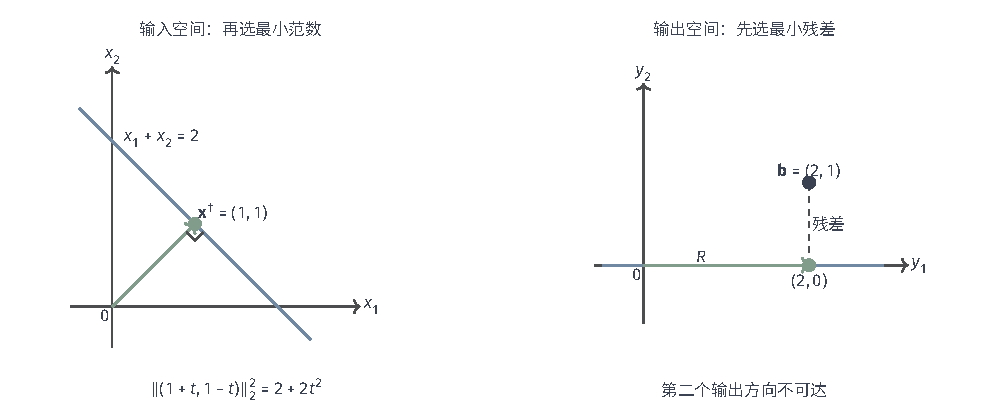
\includegraphics[width=168.998mm]{figures/01-mathematical-preliminaries-upper/02-linear-algebra-and-geometry/tikz/matrix-analysis-pseudoinverse-selections/figure.pdf}
  \caption{伪逆的两次选择。右图先在可达输出中选择离$\bm b=(2,1)^\top$最近的
 $(2,0)^\top$；左图再在整条原像直线$x_1+x_2=2$上选择最靠近原点的$(1,1)^\top$。
 两图属于不同空间，各自等比例绘制。}
 \label{fig:matrix-analysis-pseudoinverse-selections}
\end{figure*}

满列秩时，正规方程的唯一解给出
$\bm A^\dagger=(\bm A^*\bm A)^{-1}\bm A^*$；
满行秩时，$\bm A^*(\bm A\bm A^*)^{-1}\bm b$既达到$\bm b$又属于$N^\perp$，
故$\bm A^\dagger=\bm A^*(\bm A\bm A^*)^{-1}$。
这些是推导公式，不是形成逆矩阵的数值建议。一般加权问题若同时改变输出残差和输入
范数，投影与正交补也要相应改变，不能直接沿用标准伪逆。
伪逆虽对每个固定矩阵唯一，却不保证随矩阵连续，例如非零标量$\varepsilon$的伪逆
为$1/\varepsilon$，而零标量的伪逆为零；秩改变是必须检查的边界。

\subsubsection{基于矩阵分解的直接求解}
\label{sec:linear-algebra-direct-residual}

消元改变中间方程的尺度，另一条路线用正交变换保持欧氏长度。对
$\bm A\in\mathbb R^{m\times d}$、$m\geq d$且满列秩，经济型QR分解为
$\bm A=\bm Q\bm R$，其中$\bm Q\in\mathbb R^{m\times d}$满足
$\bm Q^\top\bm Q=\bm I$，$\bm R\in\mathbb R^{d\times d}$可逆上三角。
于是
\[
 \lVert\bm A\bm x-\bm b\rVert_2^2
 =\lVert\bm R\bm x-\bm Q^\top\bm b\rVert_2^2
  +\lVert(\bm I-\bm Q\bm Q^\top)\bm b\rVert_2^2.
\]
第二项不能改变，只需求解$\bm R\bm x=\bm Q^\top\bm b$。这没有构造
$\bm A^\top\bm A$；两个方法的数值差异稍后用条件数解释。

Gram--Schmidt将每列减去已有正交方向，再归一化，在精确算术中给出QR。
稠密计算常用Householder反射一次消去一列主对角线下的全部元素。对非零实向量
$\bm a$，令$s=1$当$a_1\geq0$，否则$s=-1$，并取
\[
 \bm v=\bm a+s\lVert\bm a\rVert_2\bm e_1,\qquad
 \bm H=\bm I-2\frac{\bm v\bm v^\top}{\bm v^\top\bm v}.
\]
直接相乘可验$\bm H^\top\bm H=\bm I$、
$\bm H\bm a=-s\lVert\bm a\rVert_2\bm e_1$。符号选择避免在$\bm v$首元素中相减
两个接近的数。每次只作用于剩余子块，得到
$\bm Q_{\mathrm{full}}^\top\bm A=
[\bm R^\top,\bm0^\top]^\top$；只存反射向量即可应用$\bm Q^\top$，
不必存整个$m\times m$正交矩阵。复数时选相位并使用共轭转置。

例如$\bm a=(3,4)^\top$给$\bm v=(8,4)^\top$，
$\bm H=\left[\begin{smallmatrix}-3/5&-4/5\\-4/5&3/5\end{smallmatrix}\right]$，
确实将$\bm a$送到$(-5,0)^\top$。稠密QR约需$2md^2-2d^3/3$次运算，
多个右端可以复用全部反射与$\bm R$。秩亏时仍可得到QR表示，却不能直接对奇异
$\bm R$回代；列主元QR会重新安排列以辅助判断秩，可靠阈值还需要误差尺度。
普通无主元QR的某个小对角元本身不是全部数值秩信息。

\subsubsection{基于梯度更新的迭代求解}
\label{sec:linear-algebra-gradient-residual}

矩形最小二乘要先把输出残差搬回输入端。目标
$f(\bm w)=\tfrac12\lVert\bm X\bm w-\bm y\rVert_2^2$的梯度为
$\bm X^\top(\bm X\bm w-\bm y)$，因此
\begin{equation}
 \bm w^{(t+1)}
 =\bm w^{(t)}+\eta\bm X^\top(\bm y-\bm X\bm w^{(t)}).
 \label{eq:ch06-least-squares-gradient-update}
\end{equation}
每步只需一次$\bm X$和一次$\bm X^\top$作用，不必形成Gram矩阵；
稀疏存储下成本为$O(\operatorname{nnz}(\bm X))$。
伴随搬回残差而非求逆，正是这里出现$\bm X^\top$的原因。固定步长的收敛范围和
初值如何决定选解将在第~\ref{sec:ch06-gradient-convergence}小节完整证明。

\subsection{双侧作用下的矩阵方程求解}
\label{sec:linear-algebra-matrix-equations}

未知对象也可以是一张矩阵：左乘对未知矩阵的各行作线性组合，右乘对其各列作线性组合。
例如$\bm A\bm Z\bm B=\bm C$固定$\bm A,\bm B$后对$\bm Z$线性，
式~\eqref{eq:matrix-analysis-vec-kronecker}将其编码为普通向量方程。
两端矩阵可逆时，混合乘积规则还给出
$(\bm A\otimes\bm B)^{-1}=\bm A^{-1}\otimes\bm B^{-1}$，从而可以逐侧反演。
左右作用的和仍对未知矩阵线性，但不能再把两侧分别求逆；后文求平方根的一阶响应就会遇到这种情形。
先固定左右作用矩阵，研究它们能否唯一确定未知矩阵。

\begin{definition}[Sylvester方程]
\label{def:matrix-analysis-sylvester-equation}
给定$\bm A\in\mathbb F^{m\times m}$、$\bm B\in\mathbb F^{n\times n}$和
$\bm C\in\mathbb F^{m\times n}$，关于$\bm Z\in\mathbb F^{m\times n}$的方程
\[
 \bm A\bm Z+\bm Z\bm B=\bm C
\]
称为\term{Sylvester方程}（Sylvester equation）。
\end{definition}
它的向量化形式为
$[\bm I_n\otimes\bm A+\bm B^\top\otimes\bm I_m]\operatorname{vec}(\bm Z)
=\operatorname{vec}(\bm C)$。这让向量系统的求解方法可以直接使用，也说明矩阵
未知量依然属于一个线性空间；大规模时应利用左右乘法避免存储$mn\times mn$矩阵。
例如对角$\bm A=\operatorname{diag}(1,2)$、
$\bm B=\operatorname{diag}(3,4)$时，$z_{i,j}=c_{i,j}/(a_{i,i}+b_{j,j})$。
若某个和为零，对应右端非零则无解，为零则留下自由度。一般矩阵可回用Schur表示，把左右作用同时转换为三角形式。


回用已经建立的三角化，可以求解一般矩阵方程。对
$\bm A\bm Z+\bm Z\bm B=\bm C$，分别取
$\bm A=\bm Q\bm T\bm Q^*$、
$\bm B=\bm U\bm S\bm U^*$，令
$\bm Y=\bm Q^*\bm Z\bm U$、$\bm D=\bm Q^*\bm C\bm U$，则
\[
 \bm T\bm Y+\bm Y\bm S=\bm D.
\]
逐元素有
\[
 (T_{i,i}+S_{j,j})Y_{i,j}
 =D_{i,j}-\sum_{k>i}T_{i,k}Y_{k,j}
          -\sum_{\ell<j}Y_{i,\ell}S_{\ell,j}.
\]
按列从左向右、每列自下向上计算，右侧所需元素已经得到。
因此对每个右端唯一可解的充要条件为
\begin{equation}
 \lambda_i(\bm A)+\lambda_j(\bm B)\neq0
 \quad\hbox{对所有 }i,j,\qquad
 \operatorname{spec}(\bm A)\cap\operatorname{spec}(-\bm B)=\varnothing.
 \label{eq:ch06-sylvester-spectral-separation}
\end{equation}
充分性由上述回代直接给出；必要性来自这一排序后的线性系统为三角系统，
其行列式是全部$\lambda_i+\lambda_j$的乘积。若有零因子，线性算子奇异，
便不可能对任意右端都有唯一解。例如标量方程$2z+(-2)z=c$在$c\neq0$时无解，
在$c=0$时解不唯一。实块Schur形式以小块求解替代逐元素除法，条件相同。
这不要求两个矩阵各自可逆；例如$\bm A=\bm0,\bm B=\bm I$仍唯一可解。

\section{收敛与逼近}
\label{sec:linear-algebra-convergence-approximation}

前面的求解与矩阵函数给出有限步结果，还没有回答序列的长期行为。
本节先建立有限维对象的一般收敛条件，再按序列的生成方式分别研究固定矩阵的幂与求解迭代。
最后固定目标矩阵，改变允许的秩，求出表示规模与最小逼近误差之间的关系。

\subsection{对象序列的收敛}
\label{sec:linear-algebra-sequence-convergence}

有限坐标逐项收敛，并不自动说明任意误差尺度都给出同一极限。
这里要回答的问题是：换一种范数（比如从逐项最大偏差换成欧氏长度），“收敛”与“有界、
紧致”这些结论会不会改变？在有限维空间里答案是不会——任何两种范数都只相差固定的常数
倍，因而它们定义的收敛完全一致；这也是为什么本节可以放心地在不同范数间切换。固定基$(b_1,\ldots,b_d)$，
令$\lVert x\rVert_c=\max_j|x_j|$为坐标最大范数。对任意范数$p$，三角不等式给出
$p(\sum_jx_jb_j)\leq C\lVert x\rVert_c$，其中$C=\sum_jp(b_j)$。
反三角不等式于是使$p$对坐标连续。
坐标单位球面$\lVert x\rVert_c=1$是实有限坐标中的闭有界集，复坐标可拆成实部与虚部，
由第\ref{chap:mathematical-analysis}章的有限维紧性结论，它是紧集。
连续的$p$在其上取到最小值$m$；正定性使$m>0$。缩放任意非零$x$得到
\begin{equation}
 m\lVert x\rVert_c\leq p(x)\leq C\lVert x\rVert_c.
 \label{eq:linear-algebra-finite-norm-equivalence}
\end{equation}
这证明任意两个有限维范数等价，也证明坐标收敛与范数收敛相互推出。

范数柯西列的各坐标都是标量柯西列，因而逐项有极限；有限个坐标重组为$x\in V$，
上界又保证序列在原范数下趋于$x$，所以有限维空间完备。
闭集合保留空间中已有的极限；闭子空间因而也完备。
闭有界集合在坐标下仍闭有界，每个序列存在收敛子列，子列极限留在该集合中。
这一结论不保证原序列收敛：两个不同点交替出现便是反例。

有限维线性映射的每个输出坐标是有限个输入坐标的线性组合，先有坐标范数下的有限界，
再由两端范数等价得到任意范数下的有界性。线性读取是输出维数为一的特殊情形。
范数单位球在坐标下闭有界，因而是紧集。线性映射有界，所以
$\bm x\mapsto\lVert T\bm x\rVert$连续；线性读取的绝对值也连续。
它们在单位球上均能达到最大值，所以诱导范数与对偶范数的上确界均可达到。
前文常用范数的显式界因而推广到一般有限维误差尺度；
常数依赖空间、基和范数，不能据此忽略高维误差放大。

\subsection{反复作用下的幂序列收敛}
\label{sec:linear-algebra-power-convergence}

对固定矩阵反复作用，初值$\bm x^{(0)}$在第$k$步变成$\bm A^k\bm x^{(0)}$。
要让所有初值都衰减，就必须控制整个矩阵幂；只检查某个初值的轨迹，
可能恰好没有观察到不稳定方向。下面先给出全体初值的衰减判据，再讨论单位圆边界与时变作用。


\begin{theorem}[固定矩阵幂的衰减判据]
对有限方阵$\bm A$，$\bm A^k\to\bm0$当且仅当$\rho(\bm A)<1$。
\end{theorem}
\begin{proof}
若$\bm A^k\to0$，对任一复特征向量有
$\bm A^k\bm v=\lambda^k\bm v\to0$，故$|\lambda|<1$。
反之，Jordan表示中每项都是有限次多项式乘以模小于$1$的指数，因而趋零；
零特征值块最终为零。有限块合并、再乘固定换基矩阵，仍趋零。
\end{proof}

任何诱导范数下$\lVert\bm A\rVert<1$都保证
$\lVert\bm A^k\rVert\leq\lVert\bm A\rVert^k\to0$，但不是必要条件。
固定二维例正是反例：$\lVert\bm A\bm e_2\rVert_2=\sqrt{16.25}>4$，
而式~\eqref{eq:ch06-diagonalizable-finite-trajectory}仍逐项趋零。
图~\ref{fig:ch06-transient-growth}把同一次迭代的轨迹和长度并列，显示短时放大
与长期衰减并不矛盾。

\begin{figure*}[htbp]
  \centering
  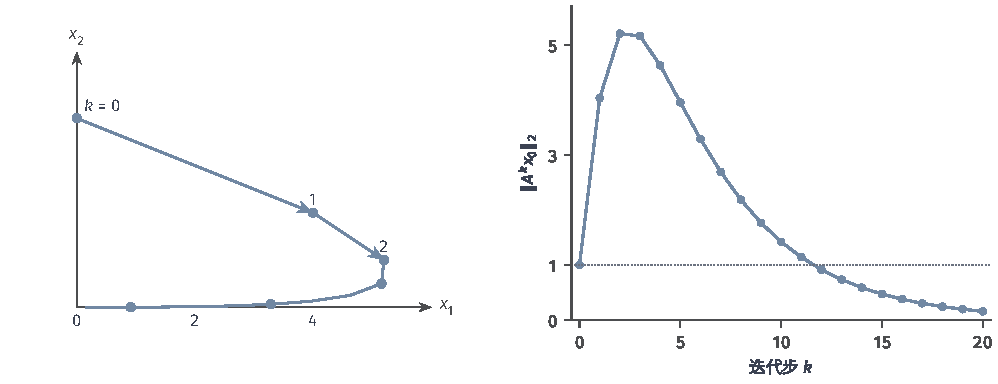
\includegraphics[width=169.0mm]{figures/01-mathematical-preliminaries-upper/02-linear-algebra-and-geometry/matplotlib/ch06-transient-growth/figure.pdf}
  \caption{固定二维矩阵的反复作用。初值为$(0,1)^\top$，前两步的长度增加，
 此后回到原点；右图将长度与初始长度$1$比较。特征值$0.8$和$0.5$决定长期衰减，
 非正交特征方向间的相消则决定早期放大。两图使用同一个矩阵和同一组迭代点。}
 \label{fig:ch06-transient-growth}
\end{figure*}

边界$\rho=1$也需区分。$\operatorname{diag}(1,0.5)^k$保留第一坐标而衰减第二坐标，
收敛到一个投影；$\operatorname{diag}(-1,0.5)^k$通常振荡；
$\left[\begin{smallmatrix}1&1\\0&1\end{smallmatrix}\right]^k$
则含线性增长的$k$项。一般矩阵幂有有限极限，当且仅当所有特征值都位于开单位圆内，
或等于$1$，且$1$的Jordan块全为$1\times1$；此时极限保留$1$特征空间上的分量。
若某特征值模大于$1$，至少有初值发散，不代表每一个初值都发散。

上述结论固定了同一个$\bm A$，不能直接推广到逐步变化的矩阵乘积。
例如两个幂零矩阵
$\bm B=\left[\begin{smallmatrix}0&2\\0&0\end{smallmatrix}\right]$、
$\bm C=\left[\begin{smallmatrix}0&0\\2&0\end{smallmatrix}\right]$
各自谱半径为零，而$\bm B\bm C=\operatorname{diag}(4,0)$，
交替作用可以增长。自适应迭代和时变系统需要检查整个乘积结构。

\subsection{求解和优化下的迭代序列收敛}
\label{sec:linear-algebra-iteration-convergence}
\label{sec:ch06-gradient-convergence}

对最小二乘，固定步长使误差更新确实由一个固定自伴矩阵控制。
但设计矩阵的零空间不进入残差，梯度也无法修改其中的初值。
为保留常用的样本平均约定，下面把
式~\eqref{eq:ch06-least-squares-gradient-update}的有效步长写成$\eta/n$。

\begin{theorem}[最小二乘梯度迭代的解选择]
\label{thm:gradient-descent-minimum-norm}
设非零$\bm X\in\mathbb R^{n\times d}$，$\bm y\in\mathbb R^n$。
对$F(\bm w)=\lVert\bm X\bm w-\bm y\rVert_2^2/(2n)$使用
\[
 \bm w^{(t+1)}
 =\bm w^{(t)}-\frac{\eta}{n}\bm X^\top(\bm X\bm w^{(t)}-\bm y),
 \qquad 0<\eta<\frac{2n}{\lVert\bm X\rVert_2^2}.
\]
任意初值均有
\begin{equation}
 \bm w^{(t)}\longrightarrow
 \bm X^\dagger\bm y+(\bm I-\bm X^\dagger\bm X)\bm w^{(0)}.
 \label{eq:matrix-analysis-gradient-limit}
\end{equation}
零初值选择唯一的最小欧氏范数最小二乘解。若进一步满行秩且$d>n$，则
\begin{equation}
 \widehat{\bm w}=\bm X^\top(\bm X\bm X^\top)^{-1}\bm y,\qquad
 \{\widehat{\bm w}\}=\argmin_{\bm X\bm w=\bm y}\lVert\bm w\rVert_2.
 \label{eq:minimum-norm-interpolator}
\end{equation}
\end{theorem}
\begin{proof}
令$\bm H=\bm X^\top\bm X$。它半正定，且
$\bm z^\top\bm H\bm z=\lVert\bm X\bm z\rVert_2^2$表明
$\ker\bm H=\ker\bm X$。其最大特征值由单位球上二次型的最大值得到
$\lambda_{\max}(\bm H)=\lVert\bm X\rVert_2^2$，这里仅用自伴谱展开与诱导范数定义。
定理~\ref{thm:matrix-analysis-pseudoinverse-minimum-norm}已经从正交几何给出
$\bm w^\dagger=\bm X^\dagger\bm y$，它满足正规方程
$\bm H\bm w^\dagger=\bm X^\top\bm y$且属于$(\ker\bm X)^\perp$。

令$\bm e^{(t)}=\bm w^{(t)}-\bm w^\dagger$，则
$\bm e^{(t+1)}=(\bm I-\eta\bm H/n)\bm e^{(t)}$。
在$\bm H$的正特征值方向$\bm q_j$上，
\[
 \bm q_j^\top\bm e^{(t)}
 =\left(1-\frac{\eta\lambda_j}{n}\right)^t
     \bm q_j^\top\bm e^{(0)}\longrightarrow0,
\]
因为步长条件使倍率绝对值小于$1$。在$\ker\bm X$上倍率为$1$，故保留
\[
 \bm P_{\ker\bm X}\bm w^{(0)}
 =(\bm I-\bm X^\dagger\bm X)\bm w^{(0)}.
\]
合并两个正交分量便得到一般极限，
整个证明不需要奇异值分解。

满行秩时全部输出可达，前述满秩伪逆公式给出$\widehat{\bm w}$，全部插值解为
\begin{equation}
 \bm w=\widehat{\bm w}+\bm v,\qquad \bm v\in\ker\bm X.
 \label{eq:interpolator-decomposition}
\end{equation}
由于$\widehat{\bm w}\perp\bm v$，
$\lVert\bm w\rVert_2^2=\lVert\widehat{\bm w}\rVert_2^2+\lVert\bm v\rVert_2^2$，
只有$\bm v=0$达到最小范数。
\end{proof}

若$\bm X=\bm0$，目标与参数无关，任意步长都保持初值；零初值仍是最小范数解，
但不能使用分母为零的步长界。例如$\bm X=[1\ \ 1]$、$y=2$时，
零初值收敛到$(1,1)^\top$；从$(3,-1)^\top$出发已满足方程，迭代始终不动。
两个解训练拟合相同，范数不同。步长端点也重要：
$\eta=2n/\lVert\bm X\rVert_2^2$时，最大特征方向的误差倍率为$-1$，
一般振荡而不收敛。

梯度例子已经区分了三种结果：目标值下降、拟合值趋近和参数趋近。
CG与GMRES也产生求解序列，但系数和搜索空间随步数变化，不能沿用固定矩阵幂的证明。
前文已经证明它们在精确算术下的有限步终止条件；
嵌套搜索空间还保证CG能量误差或GMRES残差的最优值不增。
下面进一步估计这些误差随步数下降的速度，仍先针对精确算术。初始误差为零时已经得到精确解；
下面先设初始误差非零。对对称正定$\bm A$，
CG在$\bm x^{(0)}+\mathcal K_k$中最小化能量误差。
记$\bm e^{(0)}=\bm x^{(0)}-\bm x_*$，则$\bm r^{(0)}=-\bm A\bm e^{(0)}$。
对$k\geq1$，任意候选校正可写成$q_{k-1}(\bm A)\bm r^{(0)}$，
其中$q_{k-1}$的次数不超过$k-1$，因为搜索空间由前$k$个矩阵幂作用于初始残差生成。
代入残差与误差的关系，候选误差便为
$[\bm I-\bm A q_{k-1}(\bm A)]\bm e^{(0)}$。
令$p_k(t)=1-tq_{k-1}(t)$，就得到$p_k(\bm A)\bm e^{(0)}$，
且$\deg p_k\leq k$、$p_k(0)=1$；反过来，满足这两个条件的多项式也能如此表示。
$k=0$时只有原初值，对应$p_0=1$。因此
\[
 \frac{\lVert\bm e^{(k)}\rVert_{\bm A}}{\lVert\bm e^{(0)}\rVert_{\bm A}}
 \leq\min_{\substack{\deg p\leq k\\p(0)=1}}
        \max_{\lambda\in\operatorname{spec}(\bm A)}|p(\lambda)|.
\]
令$a=\lambda_{\min}>0,b=\lambda_{\max}$，并记谱端点之比为$\kappa_2(\bm A)=b/a$；
这是欧氏范数下的矩阵条件数，其一般定义将在扰动分析中给出。若$a<b$，选择
$p(\lambda)=T_k((a+b-2\lambda)/(b-a))/T_k((a+b)/(b-a))$，
其中$T_k(\cos\theta)=\cos(k\theta)$为Chebyshev多项式。
它在$[a,b]$上的分子绝对值不超过$1$；
利用$x>1$时$T_k(x)=((x+\sqrt{x^2-1})^k+(x-\sqrt{x^2-1})^k)/2$，
得到经典界
\begin{equation}
 \lVert\bm e^{(k)}\rVert_{\bm A}
 \leq2\left(\frac{\sqrt{\kappa_2(\bm A)}-1}
                 {\sqrt{\kappa_2(\bm A)}+1}\right)^k
       \lVert\bm e^{(0)}\rVert_{\bm A}.
 \label{eq:ch06-cg-condition-bound}
\end{equation}
$a=b$时$\bm A=a\bm I$，一次更新就精确求解。
这个界只利用谱端点；特征值聚簇时，在实际谱点上选多项式可给更快收敛。
采用正定预条件$\bm M$后，对称化系统
$\bm M^{-1/2}\bm A\bm M^{-1/2}$的条件数进入同一证明，
不应在普通欧氏内积中把一般非对称的$\bm M^{-1}\bm A$直接当作自伴矩阵。

GMRES在初始残差非零时相应控制
\[
\frac{\lVert\bm r^{(k)}\rVert_2}{\lVert\bm r^{(0)}\rVert_2}
\leq\min_{p(0)=1,\deg p\leq k}\lVert p(\bm A)\rVert_2.
\]
非正规矩阵的这一范数不由特征值模单独决定；对角化时还出现特征向量基的放大因子，
与本章短时放大例中的问题相同。重启、预条件和有限精度又会改变实际进展。
预条件的总成本应包括构造、每次辅助求解及存储，不能只比较迭代步数。

\subsection{秩约束下的矩阵逼近}
\label{sec:matrix-analysis-svd-low-rank}
\label{sec:ch06-rank-constrained-approximation}
\label{sec:ch06-error-constrained-rank}

一个$m\times n$稠密矩阵需要存储$mn$个数，每次作用需要$O(mn)$次运算。
在大规模问题里这往往成为瓶颈：一张推荐系统的评分矩阵或一幅图像，$mn$轻易达到百万级，
直接存储和运算都不现实。但这类矩阵的信息常高度集中——少数几个方向就解释了大部分作用，
于是自然想知道：能否只保留最重要的$k$个方向、用远少于$mn$的参数近似整张矩阵？
若能以$k$个输入输出方向的配对近似它，存储和作用成本便可降到$O((m+n)k)$。
这里把近似矩阵的秩作为规模预算：先规定误差怎样衡量，再决定保留哪些方向。
特征向量要求输出回到输入的同一方向，因而适合分析同一空间内的反复作用；
压缩却要问哪些输入方向的作用最值得保留，并允许输出落到另一个方向。
例如一个三维输入可以被送入二维输出，已经无法要求两端沿同一条方向；
又如评分矩阵把“用户方向”映到“影片方向”，两端本就是不同对象的坐标，谈不上同一个
特征方向。因此需要一种输入、输出两端各自独立选方向的分解，这正是奇异值分解与特征值
分解的根本区别。

所需的工具允许输入和输出各选一套正交基：有非零作用的输入基方向，分别被缩放后送入
配对的输出基方向，其余输入基方向映为零。这样既能处理矩形矩阵，也能比较舍弃方向造成的输出误差。
\begin{definition}[奇异值分解]
\label{def:matrix-analysis-svd}
矩阵$\bm A\in\mathbb F^{m\times n}$的\term{奇异值分解}
（singular value decomposition，SVD）为
\begin{equation}
 \bm A=\bm U\bm\Sigma\bm V^*,
 \label{eq:matrix-analysis-svd}
\end{equation}
其中$\bm U\in\mathbb F^{m\times m}$、$\bm V\in\mathbb F^{n\times n}$酉，
实数情形为正交矩阵，$\bm\Sigma\in\mathbb R^{m\times n}$仅主对角元可能非零。
令$q=\min(m,n)$，其对角元
$\sigma_1\geq\cdots\geq\sigma_q\geq0$称为\term{奇异值}（singular value）。
正奇异值的个数为$r=\operatorname{rank}(\bm A)$。
\end{definition}

存在性由自伴谱定理~\ref{thm:matrix-analysis-symmetric-spectral-theorem}给出。$\bm A^*\bm A\succeq0$有标准正交特征基
$\bm v_i$，正特征值记为$\sigma_i^2$。对$\sigma_i>0$定义
$\bm u_i=\bm A\bm v_i/\sigma_i$，则
\[
 \bm u_i^*\bm u_j
 =\frac{\bm v_i^*\bm A^*\bm A\bm v_j}{\sigma_i\sigma_j}
 =\delta_{i,j}.
\]
零特征值方向满足$\lVert\bm A\bm v_i\rVert_2^2=0$，故映为零。
把已得$\bm u_i$补成输出空间的标准正交基，即有完整SVD。
构造同时证明
\begin{equation}
 \bm A=\sum_{i=1}^r\sigma_i\bm u_i\bm v_i^*
       =\bm U_r\bm\Sigma_r\bm V_r^*.
 \label{eq:matrix-analysis-svd-rank-one-sum}
\end{equation}
后一种紧致SVD的因子尺寸依次为$m\times r$、$r\times r$和$r\times n$。
经济型或薄SVD保留$q$个方向，尺寸依次为$m\times q$、$q\times q$和$q\times n$，
其中仍可能有零奇异值。三种形式都精确表示同一个矩阵，尚未做近似。
零矩阵的紧致和为空，完整SVD的两套基可任意选择。

几何上，$\bm V^*$记录输入方向，$\bm\Sigma$按$\sigma_i$伸缩，
$\bm U$把结果送入输出方向。因此
\[
 \ker\bm A=\operatorname{span}\{\bm v_{r+1},\ldots,\bm v_n\},\qquad
 \operatorname{range}(\bm A)=\operatorname{span}\{\bm u_1,\ldots,\bm u_r\},
\]
另两组方向分别给行空间和左零空间。
对非负自伴矩阵，左右奇异方向可以相同；对不定自伴矩阵，奇异值取特征值的绝对值，
符号由左右方向吸收。一般非正规方阵的奇异方向并非特征方向，
矩形矩阵甚至没有通常意义的特征值。
若若干正奇异值相等，对应左右向量可同步酉旋转，分解结果不变；
完整谱簇的左右子空间确定，单个基向量却不唯一。

图~\ref{fig:matrix-analysis-svd-geometry}使用二维旋转矩阵
$\bm R(\theta)=
\left[\begin{smallmatrix}\cos\theta&-\sin\theta\\\sin\theta&\cos\theta\end{smallmatrix}\right]$
构造一个左右方向不同的变换，两侧采用相同比例便于比较伸缩量。

\begin{figure*}[htbp]
  \centering
  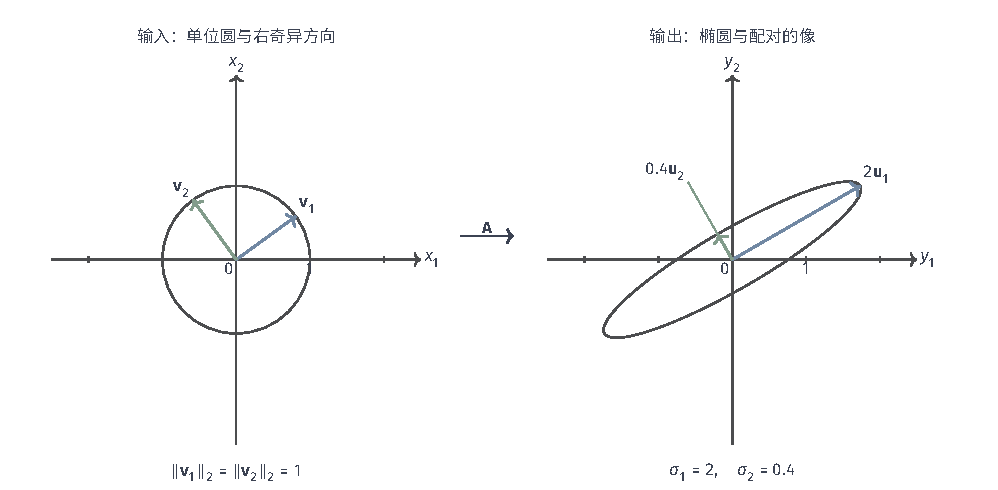
\includegraphics[width=168.998mm]{figures/01-mathematical-preliminaries-upper/02-linear-algebra-and-geometry/tikz/matrix-analysis-svd-geometry/figure.pdf}
  \caption{矩阵$\bm A=\bm R(\pi/6)\operatorname{diag}(2,0.4)\bm R(\pi/5)^\top$
 将单位圆变为椭圆。蓝、绿分别对应两个奇异方向；同色箭头在左侧标出$\bm v_i$，
 在右侧标出其像$\sigma_i\bm u_i$。两侧坐标比例相同。奇异值决定长度变化，左右方向可以不同，
 因而这不是沿特征方向的同空间缩放。图为教学构造。}
 \label{fig:matrix-analysis-svd-geometry}
\end{figure*}

为看清近共线样本的两个尺度，把式~\eqref{eq:linear-algebra-nearly-collinear-design}
的输出限制到$\operatorname{span}\{\bm c_1,\bm q\}$，用
$\bm c_1/\sqrt3,\bm q/\sqrt2$作正交坐标，再将全部输出统一除以$\sqrt3$，
得到二维表示
\begin{equation}
 \bm X_{\widetilde\varepsilon}
 =\begin{bmatrix}1&1\\0&\widetilde\varepsilon\end{bmatrix},
 \qquad \widetilde\varepsilon=\sqrt{2/3}\,\varepsilon.
 \label{eq:matrix-analysis-nearly-collinear-design}
\end{equation}
这一统一缩放也把奇异值除以$\sqrt3$，不改变它们的比值。
为同时追踪设计和响应，把上述输出转换记为
\[
 T\bm z=\left(\frac{\bm c_1^\top\bm z}{3},
                   \frac{\bm q^\top\bm z}{\sqrt6}\right)^\top.
\]
于是$T\bm X_\varepsilon=\bm X_{\widetilde\varepsilon}$，
原响应$\bm y=\bm c_1+\delta\bm q$变成
$T\bm y=(1,\sqrt{2/3}\delta)^\top$。
输入系数没有换坐标，故原系数$(1-\delta/\varepsilon,\delta/\varepsilon)^\top$
仍给出这份新响应。后面的扰动试验另选$(2,0)^\top$，对应原输出$2\bm c_1$；
它与当前响应不同，目的是让未扰动系数简化为$(2,0)^\top$，单独观察弱方向上的新增误差。

二维Gram矩阵为
$\bm G_{\widetilde\varepsilon}
=\left[\begin{smallmatrix}1&1\\1&1+\widetilde\varepsilon^2\end{smallmatrix}\right]$，
其两个特征值由二次方程得到
\begin{equation}
 \lambda_\pm
 =\frac{2+\widetilde\varepsilon^2
          \mathbin{\pm}\sqrt{4+\widetilde\varepsilon^4}}{2}.
 \label{eq:matrix-analysis-nearly-collinear-gram-eigenvalues}
\end{equation}
对$\widetilde\varepsilon>0$，$\sigma_\pm=\sqrt{\lambda_\pm}$；
当$\widetilde\varepsilon\to0$时
$\sigma_{\max}\to\sqrt2$、$\sigma_{\min}\sim\widetilde\varepsilon/\sqrt2$。
大方向近似为两个系数一起变化，小方向近似为两个系数相消。
这个推导用于理解谱，不建议为计算小奇异值显式形成Gram矩阵，
也不建议直接用相近两数相减计算$\lambda_-$；后面的误差分析会解释原因。

现在可以把已定义的伪逆写成奇异坐标形式：
\begin{equation}
 \bm A^\dagger
 =\bm V_r\bm\Sigma_r^{-1}\bm U_r^*
 =\sum_{i=1}^r\sigma_i^{-1}\bm v_i\bm u_i^*.
 \label{eq:matrix-analysis-pseudoinverse}
\end{equation}
这不是另立一种选解原则。输出的左零空间分量先被消去，其余$\bm u_i$分量除以
$\sigma_i$并映回$\bm v_i$，正是零空间正交补上的限制逆。
当重复奇异值使基改变时，同步旋转保持上式不变。
小$\sigma_i$在正向作用中压缩，在反求中则放大噪声。

若要把方向变化与非负伸缩分成两步，不必保留两套坐标矩阵的全部信息。
\begin{definition}[极分解与部分等距因子]
\label{def:matrix-analysis-polar-decomposition}
矩阵$\bm A\in\mathbb F^{m\times n}$的规范\term{极分解}（polar decomposition）为
\begin{equation}
 \bm A=\bm Q\bm H,\qquad
 \bm H=(\bm A^*\bm A)^{1/2},
 \label{eq:matrix-analysis-polar-decomposition}
\end{equation}
其中$\bm H\succeq0$，$\bm Q$在$(\ker\bm A)^\perp$上保持长度，
并在$\ker\bm A$上取零。这样的$\bm Q$称为相应的部分等距因子。
\end{definition}
紧致SVD给出$\bm H=\bm V_r\bm\Sigma_r\bm V_r^*$、
$\bm Q=\bm U_r\bm V_r^*$，故
$\bm Q^*\bm Q=\bm P_{(\ker\bm A)^\perp}$、
$\bm Q\bm Q^*=\bm P_{\operatorname{range}(\bm A)}$。
$\bm H$由唯一半正定平方根确定，$\bm Q$在$\operatorname{range}(\bm H)$上
被$\bm A=\bm Q\bm H$确定，在其正交补取零，因而也唯一。
可逆方阵时$\bm Q$酉；秩亏时它不是整个输入空间的等距映射。
若维数允许把$\bm Q$进一步延拓到零空间，原矩阵并不规定零方向的像，延拓可能不唯一。
例如$\operatorname{diag}(2,0)$的规范$\bm Q=\operatorname{diag}(1,0)$，
而正交延拓$\operatorname{diag}(1,1)$和$\operatorname{diag}(1,-1)$
乘以同一$\bm H$都给原矩阵。极分解常用于形状对齐和正交约束计算，
不应把这种延拓自由误认为规范部分等距因子也不唯一。

SVD还补齐第~\ref{sec:matrix-analysis-norms-effective-rank}节中范数的谱表达。
因为酉矩阵保持欧氏长度，且迹可循环换序，
\begin{align}
 \lVert\bm A\rVert_2
 &=\max_{\lVert\bm x\rVert_2=1}\lVert\bm A\bm x\rVert_2=\sigma_1,
 \label{eq:matrix-analysis-spectral-norm}\\
 \lVert\bm A\rVert_{\mathrm F}
 &=\left(\operatorname{tr}(\bm A^*\bm A)\right)^{1/2}
   =\left(\sum_i\sigma_i^2\right)^{1/2},
 \label{eq:matrix-analysis-frobenius-norm}\\
 \lVert\bm A\rVert_*
 &:=\sum_i\sigma_i.
 \label{eq:matrix-analysis-nuclear-norm}
\end{align}
最后一项是\term{核范数}（nuclear norm），将各奇异尺度线性相加。
这里下标$*$表示矩阵核范数，不是先前对任意向量范数的抽象对偶记号；
恰好相对于Frobenius配对，它又是谱范数的对偶。

\begin{definition}[Schatten范数]
\label{def:matrix-analysis-schatten-norm}
对$1\leq p<\infty$，\term{Schatten $p$范数}（Schatten $p$-norm）为
$\lVert\bm A\rVert_{S_p}=(\sum_i\sigma_i^p)^{1/p}$；
对$p=\infty$取$\lVert\bm A\rVert_{S_\infty}=\sigma_1$，零矩阵的值为零。
\end{definition}
$p=1,2,\infty$依次给核范数、Frobenius范数和谱范数。
它们在输入输出两端的酉换基下不变，故只关心变换的伸缩谱。
$0<p<1$沿用同一公式得到的是拟范数：对
$\bm A=\operatorname{diag}(1,0)$、$\bm B=\operatorname{diag}(0,1)$，
$\lVert\bm A+\bm B\rVert_{S_p}=2^{1/p}>2$，违反三角不等式。
行分组混合范数则依赖坐标，并不属于这个族。

对$p\geq1$，三角不等式可以由矩阵配对的对偶形式理解。两个同尺寸矩阵有
$|\operatorname{tr}(\bm B^*\bm A)|
\leq\sum_i\sigma_i(\bm B)\sigma_i(\bm A)$。
具体地，分别将$\bm A,\bm B$的左右奇异向量记为
$\bm u_i,\bm v_i$与$\widetilde{\bm u}_j,\widetilde{\bm v}_j$。
展开迹并取绝对值后，第$i,j$项的权重是
$c_{i,j}=|\bm u_i^*\widetilde{\bm u}_j|\,|\bm v_i^*\widetilde{\bm v}_j|$。
固定$i$，Cauchy--Schwarz给出
\[
 \sum_jc_{i,j}\leq
 \left(\sum_j|\bm u_i^*\widetilde{\bm u}_j|^2\right)^{1/2}
 \left(\sum_j|\bm v_i^*\widetilde{\bm v}_j|^2\right)^{1/2}\leq1.
\]
最后一步使用正交投影不增加长度：两个括号分别是单位向量在一组正交方向上的投影长度。
交换两组向量，同样得到每列之和不超过$1$。
这个权重约束为何给出迹上界，还需要展开一步。令$q=\min(m,n)$，
$\alpha_i=\sigma_i(\bm A)$、$\beta_i=\sigma_i(\bm B)$均降序排列，
并补$\alpha_{q+1}=\beta_{q+1}=0$。记前$k$行、前$\ell$列的权重和为$C_{k,\ell}$。
各行、各列的和不超过$1$，所以$C_{k,\ell}\leq\min(k,\ell)$。
将奇异值写成相邻差分的和，便有
\[
 \begin{aligned}
 \sum_{i,j=1}^q\alpha_i\beta_jc_{i,j}
 &=\sum_{k,\ell=1}^q(\alpha_k-\alpha_{k+1})
                      (\beta_\ell-\beta_{\ell+1})C_{k,\ell}\\
 &\leq\sum_{k,\ell=1}^q(\alpha_k-\alpha_{k+1})
                      (\beta_\ell-\beta_{\ell+1})\min(k,\ell)
 =\sum_{i=1}^q\alpha_i\beta_i.
 \end{aligned}
\]
最后一个等式用$\min(k,\ell)=\sum_i\mathbf1\{i\leq k,\ i\leq\ell\}$展开，
再分别求两侧的差分和。因此上述配对上界成立。
再用标量Hölder不等式，得到Schatten配对界。
要证明上界能够达到，以下改用$q$表示满足$1/p+1/q=1$的共轭指数。
设$\bm A\neq0$，并令$\bm B$与$\bm A$使用相同的左右奇异向量。
对$1<p<\infty$，取$\bm B$的奇异值为
$b_i=\sigma_i(\bm A)^{p-1}/\lVert\bm A\rVert_{S_p}^{p-1}$。
由$(p-1)q=p$可验$\sum_i b_i^q=1$，且
$\sum_i b_i\sigma_i(\bm A)=\lVert\bm A\rVert_{S_p}$。
$p=1$时，在每个正奇异方向取$b_i=1$，其余取零；$p=\infty$时，只在一个最大奇异方向取$b_i=1$。
两种端点同样满足$\lVert\bm B\rVert_{S_q}=1$并达到所需配对值。
$\bm A=0$时全部配对为零，取$\bm B=0$即可。因此
\[
 \lVert\bm A\rVert_{S_p}
 =\max_{\lVert\bm B\rVert_{S_q}\leq1}
       |\operatorname{tr}(\bm B^*\bm A)|,\qquad 1/p+1/q=1.
\]
线性配对的最大值满足三角不等式；正定性与齐次性由奇异值直接验证。
这同时解释了核范数作为凸惩罚的合法性。

对秩为$r$的矩阵，标量范数比较给
\begin{equation}
 \lVert\bm A\rVert_2\leq\lVert\bm A\rVert_{\mathrm F}
 \leq\sqrt r\,\lVert\bm A\rVert_2,\qquad
 \lVert\bm A\rVert_{\mathrm F}\leq\lVert\bm A\rVert_*
 \leq\sqrt r\,\lVert\bm A\rVert_{\mathrm F}.
 \label{eq:matrix-analysis-norm-rank-relations}
\end{equation}
范数等价仍带有秩相关常数。特别是多个方向都被舍弃时，最坏方向误差和总平方误差
不能用同一个舍弃奇异值替代。


先固定秩预算$k$，在所有秩不超过$k$的矩阵中寻找最小误差。
“保留最大的$k$个奇异值”需要证明，因为候选并不限于删去原分解中的若干项，
还可以采用任意新的方向。为建立最优性，先把单方向和子空间的能量选择写清。

\begin{definition}[Rayleigh商]
\label{def:matrix-analysis-rayleigh-quotient}
对自伴矩阵$\bm A$和非零向量$\bm x$，
\begin{equation}
 R_{\bm A}(\bm x)=\frac{\bm x^*\bm A\bm x}{\bm x^*\bm x}
 \label{eq:matrix-analysis-rayleigh-quotient}
\end{equation}
称为\term{Rayleigh商}（Rayleigh quotient），即单位平方长度对应的二次型强度。
\end{definition}
除以长度后，同一方向的不同缩放得到同一数值；这让方向之间可以比较。
\begin{theorem}[Rayleigh--Ritz变分原理]
\label{thm:matrix-analysis-rayleigh-ritz}
设自伴$\bm A$的特征值降序排列为$\lambda_1\geq\cdots\geq\lambda_d$，则
\begin{equation}
 \lambda_d=\min_{\bm x\neq0}R_{\bm A}(\bm x),\qquad
 \lambda_1=\max_{\bm x\neq0}R_{\bm A}(\bm x).
 \label{eq:matrix-analysis-rayleigh-ritz}
\end{equation}
两端分别由最小、最大特征值的非零特征向量达到。
\end{theorem}
\begin{proof}
写$\bm x=\sum_i c_i\bm q_i$，谱定理给
$R_{\bm A}(\bm x)=\sum_i\lambda_i|c_i|^2/\sum_i|c_i|^2$。
它是特征值的凸组合，位于两端之间；取相应特征向量即达到端点。
\end{proof}
例如$R_{\bm X^*\bm X}(\bm z)=
\lVert\bm X\bm z\rVert_2^2/\lVert\bm z\rVert_2^2$，
所以近共线Gram矩阵的$\lambda_-$确实量化最弱输入方向，
不只是特征多项式的一个根。

要评价中间的第$i$个方向，需比较维数受约束的整个子空间。
\begin{theorem}[Courant--Fischer极小极大原理]
\label{thm:matrix-analysis-courant-fischer}
在上述降序约定下，对$i=1,\ldots,d$，
\begin{equation}
 \lambda_i
 =\max_{\dim S=i}\ \min_{\substack{\bm x\in S\\\bm x\neq0}}R_{\bm A}(\bm x)
 =\min_{\dim T=d-i+1}\ \max_{\substack{\bm x\in T\\\bm x\neq0}}R_{\bm A}(\bm x).
 \label{eq:matrix-analysis-courant-fischer}
\end{equation}
\end{theorem}
\begin{proof}
记$E_i=\operatorname{span}\{\bm q_1,\ldots,\bm q_i\}$、
$F_i=\operatorname{span}\{\bm q_i,\ldots,\bm q_d\}$。
任意$i$维$S$与$F_i$有非零交向量，其Rayleigh商不超过$\lambda_i$，
所以第一个极值不超过$\lambda_i$；取$S=E_i$时，所有非零向量的商都不小于
$\lambda_i$，等号达到。任意$d-i+1$维$T$与$E_i$也有非零交向量，
其商不小于$\lambda_i$，故第二个极值不小于$\lambda_i$；
取$T=F_i$时，所有商不超过$\lambda_i$，再次达到等号。
\end{proof}

固定$k$维子空间以后，总能量还可以用迹比较。
若$\bm W^*\bm W=\bm I_k$，把各列展开到特征基，令
$p_i=\sum_{j=1}^k|(\bm q_i^*\bm W)_j|^2$，则
$0\leq p_i\leq1$、$\sum_i p_i=k$，且
$\operatorname{tr}(\bm W^*\bm A\bm W)=\sum_i\lambda_i p_i$。
将权重从小特征值方向移到尚未饱和的大特征值方向，不会减小目标，因此
\[
 \max_{\bm W^*\bm W=\bm I_k}\operatorname{tr}(\bm W^*\bm A\bm W)
 =\sum_{i=1}^k\lambda_i.
\]
前$k$个特征向量达到上界。若边界特征值相等，可以在重特征空间中改变所保留的方向；
最佳值确定，并不自动给唯一子空间。

在能量代表惩罚时，所需的是相反极值，列间正交约束同样不能省。
\begin{theorem}[正交列约束下的迹最小化]
\label{thm:matrix-analysis-trace-minimum}
设实对称$\bm B$的特征值在本定理中按升序记为
$\lambda_1\leq\cdots\leq\lambda_d$，对应标准正交特征向量为$\bm u_i$。
对$1\leq k\leq d$，
\begin{equation}
 \min_{\substack{\bm H\in\mathbb R^{d\times k}\\\bm H^\top\bm H=\bm I_k}}
 \operatorname{tr}(\bm H^\top\bm B\bm H)=\sum_{i=1}^k\lambda_i.
 \label{eq:matrix-analysis-trace-minimum}
\end{equation}
前$k$个特征向量达到最小值。若$k<d$且$\lambda_k<\lambda_{k+1}$，
最优列空间唯一，但其正交基仍可右乘任意$k\times k$正交矩阵。
\end{theorem}
\begin{proof}
令$\bm C=\bm U^\top\bm H$，则$\bm C^\top\bm C=\bm I_k$，
$\bm C\bm C^\top$为秩$k$的正交投影，其对角元
$p_i=\sum_j c_{i,j}^2$满足$0\leq p_i\leq1$及$\sum_i p_i=k$。
对$k<d$，
\[
 \sum_i\lambda_i p_i-\sum_{i=1}^k\lambda_i
 =\sum_{i\leq k}\lambda_i(p_i-1)+\sum_{i>k}\lambda_i p_i
 \geq(\lambda_{k+1}-\lambda_k)\sum_{i>k}p_i\geq0.
\]
取前$k$个方向使$p_i$依次为$1$与$0$，达到下界。
有严格间隙时，等号要求所有$i>k$的$p_i=0$，故列空间必须为所述子空间。
$k=d$时$\bm H$方阵正交，迹恒为$\operatorname{tr}(\bm B)$。
\end{proof}
例如$\bm B=\operatorname{diag}(0,1,4)$、$k=2$时最小迹是$1$。
若只要求每列单位长度，两列都取$(1,0,0)^\top$会得到$0$，
但它们只张成一维，已不满足原来的规模约束。

误差几何改变时，单位方向也会改变。若成本是$\bm x^\top\bm B\bm x$，
收益是$\bm x^\top\bm A\bm x$，应比较单位成本下的收益。
\begin{definition}[对称正定矩阵对的广义特征值]
\label{def:matrix-analysis-generalized-eigenvalue}
设$\bm A^\top=\bm A$、$\bm B^\top=\bm B\succ0$。非零$\bm v$满足
\begin{equation}
 \bm A\bm v=\lambda\bm B\bm v
 \label{eq:matrix-analysis-generalized-eigenproblem}
\end{equation}
时，$\lambda,\bm v$称为矩阵对的广义特征值与广义特征向量。
求解它们称为\term{广义特征值问题}（generalized eigenvalue problem），
相应广义Rayleigh商为
$R_{\bm A,\bm B}(\bm x)=\bm x^\top\bm A\bm x/(\bm x^\top\bm B\bm x)$。
\end{definition}
对$\bm A=\bm B=\operatorname{diag}(4,1)$，该商恒为$1$；
误用欧氏分母则得到从$1$到$4$的范围，改变了任务的成本定义。

取Cholesky分解$\bm B=\bm L\bm L^\top$并令$\bm z=\bm L^\top\bm x$，
可将商改写成
\[
 R_{\bm A,\bm B}(\bm x)
 =\frac{\bm z^\top(\bm L^{-1}\bm A\bm L^{-\top})\bm z}
        {\bm z^\top\bm z}.
\]
中间矩阵对称，故所有广义特征值实，且Rayleigh--Ritz和
Courant--Fischer原理在加权几何下成立。取其正交特征向量$\bm z_i$，
映回$\bm v_i=\bm L^{-\top}\bm z_i$，就有
$\bm v_i^\top\bm B\bm v_j=\delta_{i,j}$。
因此约束$\bm W^\top\bm B\bm W=\bm I_k$下的迹最大、最小值也分别是
最大的、最小的$k$个广义特征值之和。证明只需代入
$\bm Z=\bm L^\top\bm W$并应用刚证的普通迹极值。
理论上也可用$\bm z=\bm B^{1/2}\bm x$和
$\bm B^{-1/2}\bm A\bm B^{-1/2}$；计算中用三角求解实施换元，不显式形成逆平方根。
$\bm B$若仅半正定，非零方向上分母可能为零；若不定，分母可能变号，
甚至出现无穷或复广义特征值，不能照搬正定最值结论。

回到普通欧氏误差。定义\term{截断SVD}（truncated SVD）
\begin{equation}
 \bm A_k=\sum_{i=1}^k\sigma_i\bm u_i\bm v_i^*,\qquad 0\leq k<r,
 \label{eq:matrix-analysis-truncated-svd}
\end{equation}
其中$k=0$为空和。这一候选在两种常用误差下确实都最优\scite{eckart1936}。
\begin{theorem}[Eckart--Young--Mirsky定理]
\label{thm:matrix-analysis-best-low-rank}
对$0\leq k<r=\operatorname{rank}(\bm A)$，
\begin{align}
 \min_{\operatorname{rank}(\bm B)\leq k}\lVert\bm A-\bm B\rVert_2
 &=\sigma_{k+1},
 \label{eq:matrix-analysis-best-rank-k-spectral}\\
 \min_{\operatorname{rank}(\bm B)\leq k}\lVert\bm A-\bm B\rVert_{\mathrm F}
 &=\left(\sum_{i=k+1}^r\sigma_i^2\right)^{1/2}.
 \label{eq:matrix-analysis-best-rank-k-frobenius}
\end{align}
两个最小值均由$\bm A_k$达到；$k\geq r$时取$\bm A_k=\bm A$，最小误差为零。
\end{theorem}
\begin{proof}
任取秩不超过$k$的$\bm B$。
$S=\operatorname{span}\{\bm v_1,\ldots,\bm v_{k+1}\}$为$k+1$维，
而$\dim\ker\bm B\geq n-k$，故二者有非零交向量。
取其中单位向量$\bm x=\sum_{i=1}^{k+1}c_i\bm v_i$，则
\[
 \lVert(\bm A-\bm B)\bm x\rVert_2
 =\lVert\bm A\bm x\rVert_2
 =\left(\sum_{i=1}^{k+1}\sigma_i^2|c_i|^2\right)^{1/2}
 \geq\sigma_{k+1}.
\]
这给所有候选的谱误差下界。$\bm A-\bm A_k$的最大奇异值恰为$\sigma_{k+1}$，
故下界达到。

对Frobenius误差，令$\bm C=\bm U^*\bm B\bm V$，其列空间的正交投影为$\bm P$。
酉不变性及$\bm P\bm C=\bm C$给
\[
 \lVert\bm A-\bm B\rVert_{\mathrm F}^2
 =\lVert\bm\Sigma-\bm C\rVert_{\mathrm F}^2
 =\lVert(\bm I-\bm P)\bm\Sigma\rVert_{\mathrm F}^2
  +\lVert\bm P\bm\Sigma-\bm C\rVert_{\mathrm F}^2.
\]
这里按列使用了正交分解。第一项为全部能量减去保留能量，而
$\lVert\bm P\bm\Sigma\rVert_{\mathrm F}^2
=\sum_{i=1}^q\sigma_i^2\lVert\bm P\bm e_i\rVert_2^2$。
权重在$[0,1]$内，总和不超过$\operatorname{tr}\bm P\leq k$。
依照迹最大化的权重论证，它不超过$\sum_{i=1}^k\sigma_i^2$，
所以误差平方至少为尾能量$\sum_{i>k}\sigma_i^2$。
取$\bm C$为截断后的$\bm\Sigma$使第二项为零，并保留前$k$个方向，
同时达到该下界。
\end{proof}

谱误差控制任意单位输入的最坏输出误差；Frobenius误差是对一组标准正交输入的
输出误差平方求和后开方。它们的最优值不同，不能只说“截断误差等于小奇异值”。
例如$\operatorname{diag}(2,0.4)$的秩一误差在两种范数下恰好都是$0.4$，
因为只舍弃一个方向。若有多个尾方向，则须分别取最大值或平方和。
其他加权、逐元素或分组误差需要重新核对最优性，不能自动沿用这个定理。

Frobenius目标在$1\leq k<r$且$\sigma_k>\sigma_{k+1}$时的最佳矩阵唯一：
严格间隙使最优保留子空间唯一，证明中的第二个平方项为零又确定其投影结果。
边界相等时可能有多个最佳矩阵。谱目标即使有严格间隙也未必唯一，例如
$\operatorname{diag}(2+t,0)$对$|t|\leq0.4$都以谱误差$0.4$
近似$\operatorname{diag}(2,0.4)$。
对近共线$\bm X_{\widetilde\varepsilon}$取$k=1$，两种误差都是
$\sigma_{\min}\sim\widetilde\varepsilon/\sqrt2$。
若该量已低于数据精度，保留第二个方向的意义有限；若弱方向含有可靠信号，
舍弃它仍会产生真实偏差。

固定有限数据的重构是同一结论的一个实例。设$\bm X\in\mathbb R^{n\times d}$
每行是一个样本，先减去样本均值，使每列之和为零。
选择$\bm W^\top\bm W=\bm I_k$，低维坐标为$\bm Z=\bm X\bm W$，
重构为$\widehat{\bm X}=\bm Z\bm W^\top$，且
\[
 \lVert\bm X-\bm X\bm W\bm W^\top\rVert_{\mathrm F}^2
 =\lVert\bm X\rVert_{\mathrm F}^2-\lVert\bm X\bm W\rVert_{\mathrm F}^2
 =\lVert\bm X\rVert_{\mathrm F}^2
  -\operatorname{tr}(\bm W^\top\bm X^\top\bm X\bm W).
\]
迹极值说明取前$k$个右奇异向量即最小化重构误差，且重构恰为$\bm X_k$。
这就是\term{主成分分析}（principal component analysis，PCA）的有限矩阵形式。
$n\geq2$时，样本协方差$\bm X^\top\bm X/(n-1)$使保留方差总和为
$\lVert\bm X\bm W\rVert_{\mathrm F}^2/(n-1)$，所以最大化保留样本方差与
最小化当前数据的平方重构误差等价。

例如取四个中心化样本
\[
 (2,0),\quad(-2,0),\quad(0,1),\quad(0,-1).
\]
Gram矩阵为$\operatorname{diag}(8,2)$。取$k=1$得到$\bm W=(1,0)^\top$，
坐标为$(2,-2,0,0)^\top$，后两个样本都重构成零，误差平方为$2$。
未中心化时，最强方向可能反映数据整体离原点的位置，而非围绕均值的变化；
重构原始数据还应加回均值。把米改成毫米也会改变该欧氏目标，是否标准化必须由任务决定。
最大样本方差不自动等于最有预测价值的方向，对总体协方差的估计保证则需要后续统计假设。

有时不直接指定$k$，而是在拟合目标中加$\lambda\lVert\bm B\rVert_*$，
或限制$\bm B=\bm L\bm R^\top$以避免存储大矩阵。
前者通过惩罚改变目标，后者用因子列数限制可行秩；它们都不能不加说明地当成同一个
固定秩截断问题。核范数与因子平方惩罚之间确有一个精确联系。
\begin{lemma}[核范数的因子分解表达]
\label{lem:matrix-analysis-nuclear-factorization}
设$\bm A\in\mathbb R^{m\times n}$，$r=\operatorname{rank}(\bm A)$。
对任意正整数$q\geq r$，
\begin{equation}
 \lVert\bm A\rVert_*
 =\min_{\substack{\bm L\in\mathbb R^{m\times q},\,
                  \bm R\in\mathbb R^{n\times q}\\\bm L\bm R^\top=\bm A}}
   \frac12\bigl(\lVert\bm L\rVert_{\mathrm F}^2+\lVert\bm R\rVert_{\mathrm F}^2\bigr).
 \label{eq:matrix-analysis-nuclear-factorization}
\end{equation}
\end{lemma}
\begin{proof}
对非零$\bm A$，写紧致SVD为$\bm P\bm\Sigma\bm Q^\top$。
取$\bm L=\bm P\bm\Sigma^{1/2}$、$\bm R=\bm Q\bm\Sigma^{1/2}$，
$q>r$时补零列，则乘积为$\bm A$，两侧平方范数均为$\sum_i\sigma_i$，
所以右侧最小值不超过核范数。
反过来，令$\bm C=\bm P\bm Q^\top$，则$\lVert\bm C\rVert_2=1$。
任意可行因子满足
\[
 \begin{aligned}
 \lVert\bm A\rVert_*
 &=\operatorname{tr}(\bm C^\top\bm A)
   =\langle\bm C^\top\bm L,\bm R\rangle_{\mathrm F}\\
 &\leq\lVert\bm C^\top\bm L\rVert_{\mathrm F}\lVert\bm R\rVert_{\mathrm F}
 \leq\lVert\bm L\rVert_{\mathrm F}\lVert\bm R\rVert_{\mathrm F}
 \leq\tfrac12\bigl(\lVert\bm L\rVert_{\mathrm F}^2+
                   \lVert\bm R\rVert_{\mathrm F}^2\bigr).
 \end{aligned}
\]
依次使用Frobenius的Cauchy--Schwarz、混合次乘性和$2ab\leq a^2+b^2$。
零矩阵时取零因子达到零，下界由非负性保证。
\end{proof}

例如$\operatorname{diag}(4,1)$的平衡因子均为$\operatorname{diag}(2,1)$，
每侧平方能量为$5$，平均后仍为核范数$5$。
把一侧乘$c$、另一侧除以$c$虽不改变乘积，却一般增加总因子能量，
这解释了“平衡”的含义。若$q<r$，精确乘积约束不可行。
因子目标关于两侧的联合变量仍非凸，恒等式不保证任意因子算法达到全局最优。
即使取$\lambda\geq0$并直接解
$\min_{\bm B}\tfrac12\lVert\bm A-\bm B\rVert_{\mathrm F}^2
+\lambda\lVert\bm B\rVert_*$，也会改变保留奇异值的大小。
令$\bm B$的奇异值为$s_i\geq0$。展开平方范数后，方向只出现在
$-\operatorname{tr}(\bm A^\top\bm B)$中；前面的奇异值配对上界说明，
固定$s_i$时，令两矩阵的左右奇异方向一致即可使目标最小。
于是只需逐个求解
\[
 \min_{s_i\geq0}\left\{\tfrac12(s_i-\sigma_i)^2+\lambda s_i\right\}.
\]
无约束极小点为$\sigma_i-\lambda$；若它小于零，非负约束使最优值落在$s_i=0$。
故$s_i=(\sigma_i-\lambda)_+=\max(\sigma_i-\lambda,0)$，即奇异值收缩，而非保留原值的截断。
惩罚参数控制收缩幅度，其产生的秩还取决于原谱，不等于直接指定$k$。


若系统规定输出误差不能超过$\tau$，应反过来求最小可行秩。
记$\sigma_{r+1}=0$，定义两条最优误差曲线
$e_2(k)=\sigma_{k+1}$、
$e_{\mathrm F}(k)=(\sum_{i>k}\sigma_i^2)^{1/2}$，
$k=0,\ldots,r$。上述低秩最优性定理已经证明它们不是某个启发式算法的误差，而是所有该规模
候选的最低误差。因此对$\tau\geq0$，
\begin{align}
 k_2(\tau)&=\min\{k\in\{0,\ldots,r\}:\sigma_{k+1}\leq\tau\}
          =\#\{i:\sigma_i>\tau\},\\
 k_{\mathrm F}(\tau)&=\min\left\{k\in\{0,\ldots,r\}:
                              \sum_{i>k}\sigma_i^2\leq\tau^2\right\}.
 \label{eq:ch06-minimum-rank-under-error}
\end{align}
截断SVD在这两个最小整数上提供可行解；任何更小秩都被最优误差下界排除。
当阈值恰好等于某奇异值时，“不超过”允许舍弃该方向，故计数用严格大于。
$\tau=0$时需要代数秩；谱误差允许秩零的条件是$\tau\geq\lVert\bm A\rVert_2$，
Frobenius误差允许秩零的条件则是$\tau\geq\lVert\bm A\rVert_{\mathrm F}$。
负阈值不可行。相对误差预算$\epsilon\geq0$也要使用对应尺度，分别令
$\tau=\epsilon\lVert\bm A\rVert_2$或$\tau=\epsilon\lVert\bm A\rVert_{\mathrm F}$，
但零矩阵应直接处理，不能计算$0/0$。

例如奇异值为$(8,3,1,0.2)$时，秩$0$至$4$的谱误差为
$(8,3,1,0.2,0)$，Frobenius误差为
$(\sqrt{74.04},\sqrt{10.04},\sqrt{1.04},0.2,0)$。
阈值$\tau=1$在谱范数下只需$k=2$，在Frobenius范数下却需$k=3$，
因为两个被舍弃方向合计的平方误差为$1.04>1$。
图~\ref{fig:ch06-error-rank-curves}用同一谱展示两种读取方式。

\begin{figure}[htbp]
  \centering
  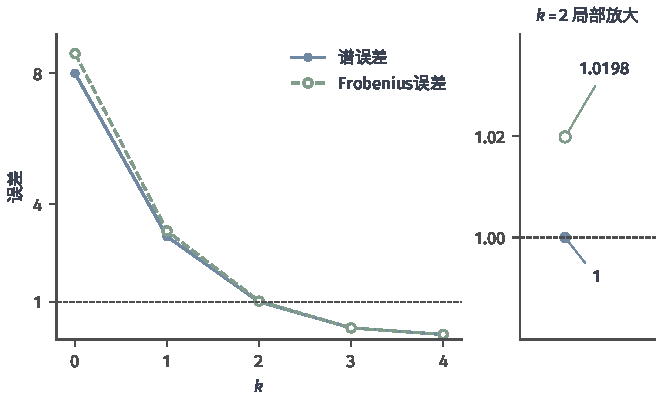
\includegraphics[width=112.0mm]{figures/01-mathematical-preliminaries-upper/02-linear-algebra-and-geometry/matplotlib/ch06-error-rank-curves/figure.pdf}
  \caption{固定奇异值$(8,3,1,0.2)$的最优误差曲线。给定横轴的秩可读出最低误差；
 给定水平误差阈值则寻找第一个满足要求的整数秩。$\tau=1$时，蓝色谱误差在
 $k=2$达标，绿色Frobenius误差要到$k=3$才达标。连线只辅助阅读，可行秩为整数。}
 \label{fig:ch06-error-rank-curves}
\end{figure}

以紧致因子存储$\bm A_k$需要约$(m+n)k+k$个数，作用于一个输入可先算
$\bm V_k^*\bm x$、按$\sigma_i$缩放、再乘$\bm U_k$。
只有当$k$相对两端维数足够小时，才真正节省存储和计算；小矩阵中因子开销可能更大。
求SVD本身也有成本，不能只统计后续乘法。噪声尺度若高于最后保留的奇异值，
把$k$算得很精确也不等于方向可辨认，这需要下一节的谱隙条件。

秩还有几种用途不同的替代尺度。代数秩严格计算非零奇异值个数，
对任意小的秩增加扰动都可能跳变。
给定绝对阈值$\tau$的\term{数值秩}（numerical rank）
$r_{\mathrm{num}}(\bm A;\tau)=\#\{i:\sigma_i>\tau\}$，
在这里等于谱范数误差阈值下的最优秩；若采用相对阈值，必须同时说明所乘尺度，
不能把“数值秩”当成一个不含容差的固定数值。

\begin{definition}[稳定秩]
\label{def:matrix-analysis-stable-rank}
非零矩阵$\bm A$的\term{稳定秩}（stable rank）为
\begin{equation}
 r_{\mathrm{stable}}(\bm A)
 =\frac{\lVert\bm A\rVert_{\mathrm F}^2}{\lVert\bm A\rVert_2^2}
 =\frac{\sum_i\sigma_i^2}{\sigma_1^2}.
 \label{eq:matrix-analysis-stable-rank}
\end{equation}
零矩阵另约定为零。
\end{definition}
对非零矩阵，它在$[1,r]$内，所有非零奇异值相等时取$r$，能量集中在首方向时接近$1$。
它在非零矩阵处连续且不随整体缩放改变，但在零矩阵处的上述约定不使它连续。
近共线例有
$r_{\mathrm{stable}}(\bm X_{\widetilde\varepsilon})
=1+\lambda_-/\lambda_+\to1$，而$\widetilde\varepsilon>0$时的代数秩始终为$2$。

稳定秩是\term{有效秩}（effective rank）的一种。
另一种常用口径对非零矩阵先令$p_i=\sigma_i/\sum_j\sigma_j$，再定义
$r_{\mathrm{ent}}=\exp(-\sum_i p_i\log p_i)$，约定$0\log0=0$；
也有用平方奇异值归一化的版本，其值一般不同。
这些连续尺度不是误差阈值下的最优整数秩。例如上述四个奇异值的稳定秩是
$74.04/64\approx1.157$，既不是$\tau=1$时的$2$，也不是$3$。
它也不同于第~\ref{chap:functional-analysis-and-approximation}章随正则化尺度
变化的核有效维度$d_{\mathrm{eff}}(\lambda)$。

各层变换还满足
$\lVert\bm A_L\cdots\bm A_1\rVert_2\leq\prod_{\ell=1}^L\lVert\bm A_\ell\rVert_2$，
但逐层最强方向未必能对齐，上界可能宽松；
稳定秩不能按同一方式简单相乘。由此也可见，规模指标、最优误差与实际可辨认信息
是不同结论。接下来需要问：数据或计算发生微小变化时，这些答案还可靠吗？

\section{扰动与稳定性}
\label{sec:linear-algebra-stability}
\label{sec:matrix-analysis-conditioning-perturbation}


近共线例中的两个系数可能很大，下一步要问：测量稍变以后，它们会变多少？
这里要先分清两种来源完全不同的误差，否则容易错误地归咎于算法：一种是问题本身“敏感”——
哪怕用完美算术，只要输入数据有一点测量误差，精确解也会剧烈变化（这由条件数刻画，与算法
无关）；另一种是同一输入在有限精度机器上算错了（这才是算法的舍入误差）。
即使输入保持不变，有限精度计算还可能产生另一项误差。
本节先把问题敏感性与计算误差拆开，再分别分析线性方程解、谱分解与矩阵函数的响应。
每种任务都要指定所比较的输出；解向量、谱子空间与函数矩阵需要的稳定性条件不同。

\subsection{运算的误差传播}
\label{sec:linear-algebra-error-propagation}
\label{sec:ch06-error-propagation}


设目标映射为$F$，理想输入为$z$，实际交给算法的是$z+\Delta z$，
算法返回$\widehat y$。一个确定的误差分解是
\[
 \widehat y-F(z)
 =\underbrace{\widehat y-F(z+\Delta z)}_{\text{计算误差}}
  +\underbrace{F(z+\Delta z)-F(z)}_{\text{输入变化引起的误差}}.
\]
第一项评价算法对当前输入的计算，第二项评价问题对输入的敏感性。
没有额外证据时，不能把两项都归咎于求解器。
以下讨论算法时，将实际输入重新记为$z$，以免每式都携带相同的扰动下标。

\term{前向误差}（forward error）是$\widehat y-F(z)$的大小；
\term{后向误差}（backward error）则寻找能使
$\widehat y=F(z+\delta z)$成立的最小允许输入变化。
允许改变哪些分量、用什么范数和是否保持结构，都是定义的一部分。
例如只允许改右端与同时改矩阵，得到的线性系统后向误差不同；
若要求扰动矩阵仍对称，其最小值也可能不同。

若$F$在所讨论邻域内可微，一阶变化为
$F(z+\delta z)-F(z)=DF(z)[\delta z]+o(\lVert\delta z\rVert)$。
绝对局部条件数为导数算子范数$\lVert DF(z)\rVert$；
当$z\neq0$且$F(z)\neq0$时，相对局部条件数为
$\lVert DF(z)\rVert\lVert z\rVert/\lVert F(z)\rVert$。
它们控制足够小扰动的最坏放大，不自动给有限扰动界。
如果输出为零，应报告绝对误差或明确的任务尺度；
秩变化等不连续处不能强行使用微分。

计算模型也要写明。排除上溢、下溢及无效运算后，舍入到最近可表示数的基本运算常满足
\begin{equation}
 \operatorname{fl}(a\mathbin\circ b)
 =(a\mathbin\circ b)(1+\delta),\qquad |\delta|\leq u,
 \label{eq:ch06-floating-point-model}
\end{equation}
其中$\circ$是加、减、乘或合法除法，$u$为单位舍入误差。
IEEE双精度通常有$u=2^{-53}$。这个模型比较的是当前浮点操作数的精确运算结果，
并不消除操作数本身已有的误差；两个近数相减时，这些误差相对于微小差值会很大。
次正规数、上溢、除以零等需另处理。
累积$n$个舍入因子常用$\gamma_n=nu/(1-nu)$控制，前提是$nu<1$，
所以“误差是$u$量级”仍要核对维数和传播系数。

\begin{definition}[范数意义下的后向稳定]
\label{def:matrix-analysis-backward-stability}
设输入空间给定范数。若算法对声明的非零输入类返回
$\widehat y=F(z+\delta z)$，并在充分小的$u$下满足
$\lVert\delta z\rVert/\lVert z\rVert\leq C u$，其中$C$不依赖$u$，
则称其在此误差口径下\term{后向稳定}（backward stability）。
必须说明$C$对问题规模及输入类的依赖；零输入另用绝对误差口径。
\end{definition}
后向稳定说明算法只引入小的等效输入扰动。
若条件数也适中，一阶分析便给小前向误差；条件数很大时，两者可以同时出现：
算法很好地解了一个邻近问题，结果却离当前问题的精确答案很远。
下面用逆与线性系统把这一关系变成可计算的公式。

\subsection{线性方程解的稳定性}
\label{sec:ch06-inverse-stability}
\label{sec:matrix-analysis-error-verification}

线性方程解依赖矩阵与右端。下面分别讨论普通逆给出的唯一解，
以及伪逆选出的最小范数解。未加下标的矩阵范数采用同一向量范数诱导的范数。
先看可逆方阵$\bm A$。令$\bm E$为矩阵扰动，若
$\alpha=\lVert\bm A^{-1}\rVert\lVert\bm E\rVert<1$，则
\[
 \bm A+\bm E=\bm A(\bm I+\bm A^{-1}\bm E)
\]
可逆，因为$\sum_{j\geq0}(-\bm A^{-1}\bm E)^j$绝对收敛并为右侧括号的逆。
利用逆的差恒等式，得到
\begin{equation}
 (\bm A+\bm E)^{-1}-\bm A^{-1}
 =-(\bm A+\bm E)^{-1}\bm E\bm A^{-1},\qquad
 \lVert(\bm A+\bm E)^{-1}-\bm A^{-1}\rVert
 \leq\frac{\lVert\bm A^{-1}\rVert^2\lVert\bm E\rVert}{1-\alpha}.
 \label{eq:ch06-inverse-finite-perturbation}
\end{equation}
分母表示允许扰动到奇异边界之间还保留多少余量。
$\alpha\geq1$只表示该保证失效，不意味着扰动后的矩阵必定奇异。

\begin{definition}[可逆矩阵的条件数]
\label{def:matrix-analysis-condition-number}
对同一向量范数诱导的矩阵范数，可逆方阵$\bm A$的
\term{条件数}（condition number）为
\begin{equation}
 \kappa(\bm A)=\lVert\bm A\rVert\lVert\bm A^{-1}\rVert.
 \label{eq:matrix-analysis-condition-number}
\end{equation}
\end{definition}
$\lVert\bm I\rVert=1$及次乘性保证$\kappa\geq1$。
欧氏情形由SVD给出
\begin{equation}
 \kappa_2(\bm A)=\frac{\sigma_{\max}(\bm A)}{\sigma_{\min}(\bm A)}.
 \label{eq:matrix-analysis-spectral-condition-number}
\end{equation}
酉矩阵的条件数为$1$，接近奇异时条件数增大。
将式~\eqref{eq:ch06-inverse-finite-perturbation}除以$\lVert\bm A^{-1}\rVert$，
便得到相对逆值误差不超过
$\kappa(\bm A)(\lVert\bm E\rVert/\lVert\bm A\rVert)/
(1-\kappa(\bm A)\lVert\bm E\rVert/\lVert\bm A\rVert)$。
它量化的是逆值变化，不只是某一个右端的求解误差。

满秩矩形矩阵常记$\kappa_2=\sigma_1/\sigma_q$，$q=\min(m,n)$。
秩亏矩阵在允许任意秩变化的反演问题中通常约定条件数为无穷；
固定矩阵后，伪逆线性映射却仍有有限范数
$\lVert\bm A^\dagger\rVert_2=1/\sigma_r$（$r>0$），零矩阵的伪逆范数为零。
前者讨论输入矩阵改变，后者只讨论右端改变，不能混用。

在秩保持的区域，伪逆也有有限扰动控制。令$\bm B=\bm A+\bm E$。
用Penrose投影恒等式整理可得精确关系
\[
 \begin{aligned}
 \bm B^\dagger-\bm A^\dagger
 ={}&-\bm B^\dagger\bm E\bm A^\dagger\\
 &+\bm B^\dagger(\bm B^\dagger)^*\bm E^*(\bm I-\bm A\bm A^\dagger)\\
 &+(\bm I-\bm B^\dagger\bm B)\bm E^*(\bm A^\dagger)^*\bm A^\dagger.
 \end{aligned}
\]
可先把差写成
$-\bm B^\dagger\bm E\bm A^\dagger+
\bm B^\dagger(\bm I-\bm A\bm A^\dagger)
-(\bm I-\bm B^\dagger\bm B)\bm A^\dagger$，
再用$\bm B^*=\bm A^*+\bm E^*$及正交投影消去对应零空间项，验证上式。
投影范数不超过$1$，故若两者秩同为$r>0$，且最小正奇异值都不小于$s_0>0$，则
\begin{equation}
 \lVert\bm B^\dagger-\bm A^\dagger\rVert_2
 \leq\bigl(\lVert\bm B^\dagger\rVert_2\lVert\bm A^\dagger\rVert_2
          +\lVert\bm B^\dagger\rVert_2^2
          +\lVert\bm A^\dagger\rVert_2^2\bigr)\lVert\bm E\rVert_2
 \leq\frac{3\lVert\bm E\rVert_2}{s_0^2}.
 \label{eq:ch06-pseudoinverse-fixed-rank-perturbation}
\end{equation}
同秩邻域中正奇异值不会突然降到零，后面的奇异值扰动界会给出具体余量。
若秩改变，这个统一下界可能消失。例如
$\bm A=\operatorname{diag}(1,0)$、
$\bm B_\epsilon=\operatorname{diag}(1,\epsilon)$趋向同一个$\bm A$，
却有$\bm B_\epsilon^\dagger=\operatorname{diag}(1,\epsilon^{-1})$不趋向
$\bm A^\dagger=\operatorname{diag}(1,0)$。把零奇异方向置零不保证邻近非零方向也稳定。

逆值敏感性传到求解时，还要计入右端。设$\bm A\bm x=\bm b\neq0$，
扰动系统为$(\bm A+\bm E)(\bm x+\Delta\bm x)=\bm b+\Delta\bm b$。
相减得
$\bm A\Delta\bm x=\Delta\bm b-\bm E\bm x-\bm E\Delta\bm x$。
取范数、将最后一项吸收到左侧，并用
$\lVert\bm b\rVert\leq\lVert\bm A\rVert\lVert\bm x\rVert$，得到
\begin{equation}
 \frac{\lVert\Delta\bm x\rVert}{\lVert\bm x\rVert}
 \leq
 \frac{\kappa(\bm A)}
 {1-\kappa(\bm A)\lVert\bm E\rVert/\lVert\bm A\rVert}
 \left(\frac{\lVert\bm E\rVert}{\lVert\bm A\rVert}
       +\frac{\lVert\Delta\bm b\rVert}{\lVert\bm b\rVert}\right),
 \quad \lVert\bm A^{-1}\rVert\lVert\bm E\rVert<1.
 \label{eq:matrix-analysis-linear-system-perturbation}
\end{equation}
只改右端时，$\Delta\bm x=\bm A^{-1}\Delta\bm b$，上界退化为
$\kappa(\bm A)\lVert\Delta\bm b\rVert/\lVert\bm b\rVert$。
它是最坏方向界，不是每个扰动都达到的倍数。

下面用两个手算的$2\times2$方程组说明“病态”为什么会让解不可信。
先看条件良好的情形，取$\bm A_1=\begin{bmatrix}2&0\\0&1\end{bmatrix}$。
右端从$\bm b_1=(2,1)^\top$改为$\bm b_1'=(2,1.01)^\top$，
解从$(1,1)^\top$变为$(1,1.01)^\top$：
按欧氏范数计算，右端相对变化为$0.01/\sqrt5\approx0.00447$，
解的相对变化为$0.01/\sqrt2\approx0.00707$，放大比约为$1.58$，
不超过$\kappa_2(\bm A_1)=2$。
再看两组方程中系数几乎平行的情形，取
$\bm A_2=\begin{bmatrix}1&1\\1&1+\varepsilon\end{bmatrix}$，
$\varepsilon>0$很小。第一条方程说$x_1+x_2$等于某个数，
第二条说$x_1+(1+\varepsilon)x_2$也几乎等于同一个数，
两条直线接近重合，因此解的位置对数据的微小改动非常敏感。
它的行列式为$\varepsilon$，$\kappa_2(\bm A_2)\approx4/\varepsilon$。
取$\varepsilon=10^{-4}$，右端$\bm b_2=(1,1)^\top$的解是$(1,0)^\top$。
两条方程相减得到$\varepsilon x_2=b_{2,2}-b_{2,1}$，右端的差会被除以很小的$\varepsilon$。
只把第二个分量改动$10^{-4}$，得到$\bm b_2'=(1,1+10^{-4})^\top$，
相减后的方程便给出$x_2=1$，再由第一条方程得$x_1=0$。
因此解由$(1,0)^\top$变成$(0,1)^\top$；右端相对变化为$10^{-4}/\sqrt2$，
解的相对变化为$\sqrt2$，放大比为$2\times10^4$，不超过
$\kappa_2(\bm A_2)\approx4\times10^4$，且已达到同一量级。
这两个例子中都没有出现浮点误差，差别完全来自问题本身；
条件数刻画的就是这种“输入稍变、输出剧变”的放大倍数，
而它与算法无关。因此，一个算法即使后向稳定，
在$\bm A_2$上返回的$\widehat{\bm x}$也可能离真解很远：
它可能精确解出了一个右端略有变化的邻近问题，但那个问题的答案已经与原解相差很大。
例如把上述$(0,1)^\top$代回原右端为$(1,1)^\top$的方程，残差范数仅为$10^{-4}$，
解误差范数却为$\sqrt2$。
实际判断时还应结合残差：$\bm A_2\widehat{\bm x}-\bm b$可能很小，
而$\widehat{\bm x}$与真解之差仍很大，这正是下面单独讨论残差、解误差与后向误差三种口径的原因。
伪逆选解也可直接拆成
$\bm B^\dagger(\bm b+\Delta\bm b)-\bm A^\dagger\bm b
=(\bm B^\dagger-\bm A^\dagger)\bm b+\bm B^\dagger\Delta\bm b$，
再结合式~\eqref{eq:ch06-pseudoinverse-fixed-rank-perturbation}；
零输出时应保留绝对界，不盲目除以解范数。

近共线例把系数敏感性与拟合敏感性分开。沿用二维表示
$\bm X_{\widetilde\varepsilon}$，按前面已说明的扰动试验改取响应$\bm y_0=(2,0)^\top$，
原解为$\bm\beta_0=(2,0)^\top$；改为$\bm y_0+(0,\eta)^\top$后，
\begin{equation}
 \bm\beta_0+\Delta\bm\beta
 =\begin{bmatrix}2-\eta/\widetilde\varepsilon\\
                  \eta/\widetilde\varepsilon\end{bmatrix}.
 \label{eq:matrix-analysis-collinear-coefficient-perturbation}
\end{equation}
响应相对变化$|\eta|/2$，系数相对变化
$|\eta|/(\sqrt2\,\widetilde\varepsilon)$；
$\kappa_2(\bm X_{\widetilde\varepsilon})
=\sqrt{\lambda_+/\lambda_-}\sim2/\widetilde\varepsilon$。
这是真实问题的精确敏感性，并未引入求解器。

\begin{figure}[htbp]
  \centering
  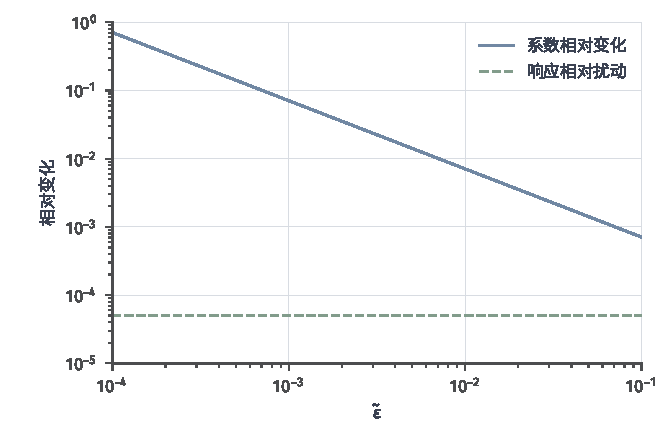
\includegraphics[width=112.0mm]{figures/01-mathematical-preliminaries-upper/02-linear-algebra-and-geometry/matplotlib/matrix-analysis-coefficient-sensitivity/figure.pdf}
  \caption{近共线矩阵的精确敏感性。固定$\bm y_0=(2,0)^\top$，
 扰动为$(0,10^{-4})^\top$；绿线是响应相对扰动$5\times10^{-5}$，
 蓝线是系数相对变化$10^{-4}/(\sqrt2\,\widetilde\varepsilon)$。
 双对数坐标显示列越接近，反求系数越敏感；图中没有数值求解误差。}
 \label{fig:matrix-analysis-coefficient-sensitivity}
\end{figure}

一般最小二乘在固定$\bm X$下的拟合值是
$\widehat{\bm y}=\bm X\bm X^\dagger\bm y=\bm P_{\bm X}\bm y$，
故$\lVert\Delta\widehat{\bm y}\rVert_2
\leq\lVert\Delta\bm y\rVert_2$。
系数变化却是$\bm X^\dagger\Delta\bm y$，可由小正奇异值放大。
该预测界只对固定训练设计成立；若设计也改变，还要计入投影变化。
新输入$\bm a$上的预测变化为
$\bm a^\top\bm X^\dagger\Delta\bm y$，
绝对值由$\lVert(\bm X^\dagger)^\top\bm a\rVert_2\lVert\Delta\bm y\rVert_2$
控制。新样本可能不遵循训练数据的近共线关系，因此外推仍可敏感。

抑制弱方向会同时改变估计。截断伪逆只保留$\sigma_i>\tau$的项，
把其余逆因子置零；对固定截断算子，右端放大不超过$1/\tau$（$\tau>0$）。
但截断阈值附近若有奇异值跨越，算子本身又可能跳变。
岭型目标$\lVert\bm X\bm w-\bm y\rVert_2^2+\lambda\lVert\bm w\rVert_2^2$
在$\lambda>0$时给出正定系统
$(\bm X^\top\bm X+\lambda\bm I)\bm w=\bm X^\top\bm y$，可用Cholesky。
也可精确改写成增广最小二乘
\[
 \min_{\bm w}\left\|
 \begin{bmatrix}\bm X\\\sqrt\lambda\,\bm I\end{bmatrix}\bm w
 -\begin{bmatrix}\bm y\\\bm0\end{bmatrix}\right\|_2^2.
\]
这两种写法对应同一个岭目标，却都不同于未正则化的原问题。选择$\lambda$是在
改变任务设定，不能仅解释为让分解“成功”的实现细节。

岭解
$\widehat{\bm\beta}_\lambda
=(\bm X^\top\bm X+\lambda\bm I)^{-1}\bm X^\top\bm y$
将逆因子替换为
\begin{equation}
 \frac{\sigma_i}{\sigma_i^2+\lambda},\qquad \lambda>0.
 \label{eq:matrix-analysis-ridge-filter-factor}
\end{equation}
由于$\sigma_i^2+\lambda\geq2\sigma_i\sqrt\lambda$，其最大放大不超过
$1/(2\sqrt\lambda)$；训练拟合在该方向上则乘以
$\sigma_i^2/(\sigma_i^2+\lambda)<1$，引入收缩偏差。
零奇异方向两种方法都给零，不能恢复已被数据消去的信息。
参数$\lambda$和阈值$\tau$还随特征单位变化，不能脱离数据缩放比较。

计算结果是否可信，需要可计算的检验量。
先设$\bm A$可逆，算法给$\widehat{\bm x}$，定义\term{残差}（residual）
\begin{equation}
 \bm r=\bm b-\bm A\widehat{\bm x}.
 \label{eq:matrix-analysis-residual}
\end{equation}
因$\bm x-\widehat{\bm x}=\bm A^{-1}\bm r$，$\bm b\neq0$时
\[
 \frac{\lVert\widehat{\bm x}-\bm x\rVert}{\lVert\bm x\rVert}
 \leq\kappa(\bm A)\frac{\lVert\bm r\rVert}{\lVert\bm b\rVert}.
\]
例如$\bm A=\operatorname{diag}(1,\epsilon)$、
$\bm b=(1,\epsilon)^\top$，$0<\epsilon\ll1$。
真解$(1,1)^\top$与候选$(1,0)^\top$的相对误差为$1/\sqrt2$，
残差$(0,\epsilon)^\top$的相对大小却是
$\epsilon/\sqrt{1+\epsilon^2}\to0$。
矩阵在第二个方向把输入差异压缩了$\epsilon$倍，反求时则要除以$\epsilon$；
$\kappa_2=1/\epsilon$正好解释了放大。残差回答方程差多少，解误差回答输入离真解多远，
后向误差则将回答这个候选精确解了一个多邻近的问题。
三个对象需要结合起来评价，小残差本身不说明弱方向的参数已经求准。

若只允许改右端，$\bm A\widehat{\bm x}=\bm b-\bm r$给出相对后向误差
$\lVert\bm r\rVert_2/\lVert\bm b\rVert_2$。
$\bm b=0$时不要加一个任意小常数造分母，可报告绝对残差，或采用联合扰动定义。
\begin{definition}[线性系统的范数型相对后向误差]
\label{def:matrix-analysis-normwise-backward-error}
对$\bm A\in\mathbb R^{m\times n}$、$\bm b\in\mathbb R^m$与候选$\widehat{\bm x}$，令
\[
 \eta_2(\widehat{\bm x};\bm A,\bm b)
 =\min\left\{\epsilon\geq0:
 \begin{array}{l}
  (\bm A+\Delta\bm A)\widehat{\bm x}=\bm b+\Delta\bm b,\\
  \lVert\Delta\bm A\rVert_2\leq\epsilon\lVert\bm A\rVert_2,\quad
  \lVert\Delta\bm b\rVert_2\leq\epsilon\lVert\bm b\rVert_2
 \end{array}\right\},
\]
其中最小化也遍历满足条件的$\Delta\bm A,\Delta\bm b$，不另要求结构保持。
\end{definition}
令$d_0=\lVert\bm A\rVert_2\lVert\widehat{\bm x}\rVert_2+\lVert\bm b\rVert_2$。
$d_0>0$时有闭式
\[
 \eta_2=\frac{\lVert\bm r\rVert_2}{d_0}.
\]
证明先由$\Delta\bm A\widehat{\bm x}-\Delta\bm b=\bm r$及三角不等式得到下界。
若$\widehat{\bm x}\neq0$，取
\[
 \Delta\bm A=
 \frac{\lVert\bm A\rVert_2}{d_0}
 \frac{\bm r\widehat{\bm x}^\top}{\lVert\widehat{\bm x}\rVert_2},
 \qquad
 \Delta\bm b=-\frac{\lVert\bm b\rVert_2}{d_0}\bm r,
\]
两者恰好按分母的两项分配残差，达到下界。
若$\widehat{\bm x}=0$且$d_0>0$，取$\Delta\bm A=0,\Delta\bm b=-\bm b$
即可；若$d_0=0$，必有$\bm b=0$和$\bm A\widehat{\bm x}=0$，约定$\eta_2=0$。
对右端$\bm b\neq0$的可逆系统，可把这个联合后向误差代入
式~\eqref{eq:matrix-analysis-linear-system-perturbation}，
当$\kappa\eta_2<1$时得到相对前向误差上界$2\kappa\eta_2/(1-\kappa\eta_2)$。

上面的矩形后向误差衡量“成为邻近精确方程的解”，并不是最小二乘算法的完整评价。
不可达输出在最优点仍可能有非零残差，应检查正规方程残差
$\bm g=\bm X^*(\bm y-\bm X\widehat{\bm x})$；
秩亏时还需检查$\bm P_{\ker\bm X}\widehat{\bm x}=0$才能确认最小范数选择。
例如$\bm X=[1\ \ 1]$、$y=2$的候选$(3,-1)^\top$方程残差为零，
却不是伪逆解$(1,1)^\top$。对固定正秩矩阵，候选在行空间内的解误差最多为
$\lVert\bm g\rVert_2/\sigma_r^2$，零空间分量另计；
这是将正规方程限制到行空间后求逆的结果。两个条件承担不同检验职责。

这些界使直接法的数值区别有了明确含义。
带部分主元LU在浮点中通常表现良好，但后向误差受消元增长影响。
若定义增长因子为消元过程中最大元素绝对值除以原矩阵最大元素绝对值，
则典型误差界含维数、$u$及该因子；它在特殊矩阵上可以很大。
主元选取控制计算过程，不能改善原问题的条件数。
Householder QR通过近正交变换工作，具有相应的范数型后向误差界；
经典Gram--Schmidt在近相关列上可能丢失正交性，改进形式或重正交化才有不同保证。
不能只因精确公式中写着$\bm Q^\top\bm Q=\bm I$就认定计算出的基满足同样等式。

Cholesky在正定、无异常算术并成功完成时有良好的后向误差性质。
接近半正定边界时，舍入可能造成非正主元；失败既可能反映真实非正定，
也可能反映尺度与计算误差。添加对角常数会改变任务，需有明确正则化依据。
满列秩矩阵的正规方程满足
\begin{equation}
 \kappa_2(\bm X^\top\bm X)=\kappa_2(\bm X)^2,
 \label{eq:matrix-analysis-normal-equation-condition-square}
\end{equation}
因为特征值是奇异值平方。
近共线例使条件数从$2/\widetilde\varepsilon$量级升为
$4/\widetilde\varepsilon^2$量级；当$\widetilde\varepsilon^2$已小于舍入尺度，
形成$1+\widetilde\varepsilon^2$甚至可能直接丢掉区分两列的信息。
QR与SVD不显式形成Gram矩阵，避免这一额外损失，但不能消除原始小奇异值带来的敏感性。
岭问题虽然可对$\bm X^\top\bm X+\lambda\bm I$作Cholesky，
高精度要求时仍可使用前面建立的增广最小二乘与QR。

停止时应按任务检查真实残差、相对后向误差及条件数估计；
递推残差可能积累舍入，应适时重新计算$\bm b-\bm A\widehat{\bm x}$，
必要时使用更高精度求残差。以该残差解校正方程并更新解称为迭代改进，
它仍依赖分解精度、条件数和残差精度，不能保证任意病态问题都恢复准确解。
若数据本身的误差已超过迭代残差，继续降低计算残差也不恢复缺失信息。

\begin{table*}[htbp]
 \centering\small
 \begin{tabularx}{\linewidth}{@{}lXX@{}}
 \toprule
 方法 & 结构与主要成本 & 精度及停止时的区别\\
 \midrule
 带主元LU & 可逆方阵；分解约$2d^3/3$，每右端$O(d^2)$
 & 后向误差含主元增长；小残差仍需结合条件数\\
 QR & 满列秩最小二乘；稠密分解$O(md^2)$，可复用反射
 & 避免形成Gram矩阵；秩判断需列主元或其他分析\\
 Cholesky & 正定方阵；约$d^3/3$，利用对称存储
 & 核对正定余量；半正定退化不直接适用\\
 SVD与伪逆 & 任意矩形；稠密分解成本通常高于QR
 & 明示小奇异值；截断要报告阈值和偏差\\
 共轭梯度 & 对称正定；每步矩阵作用与少量向量存储
 & 能量误差受谱和预条件影响；重算真实残差\\
 GMRES & 本节用于非对称可逆方阵；基存储随步数增加
 & 最小残差不等于最小解误差；重启可停滞\\
 \bottomrule
 \end{tabularx}
 \caption{在同一求解任务中比较结构、成本与可靠性。稀疏分解还需计入填充，
 迭代法还需计入预条件成本；任何稳定实现都不能消除输入问题本身的敏感性。}
 \label{tab:matrix-analysis-solver-conditions}
\end{table*}

需要整个逆的许多元素时，可以从稳定分解计算并检验逆；
若只需要$\bm A^{-1}\bm b$、$\bm b^\top\bm A^{-1}\bm b$或$\bm A^{-1}\bm U$，
应用求解器通常已足够。Woodbury等精确恒等式也应通过内层求解实施并检查条件，
不能凭等式简短就推断浮点误差较小。


\subsection{谱分解的稳定性}
\label{sec:linear-algebra-spectral-stability}
\label{sec:ch06-spectral-stability}


压缩误差由奇异值决定，但压缩方向由子空间决定；前者稳定不保证后者稳定。
比较方向之前还要排除基选择的任意性。单个特征向量可改符号或复相位，
重复谱值中的整组基还可以旋转；逐列相减会把这些无实质变化的选择也计作误差。

\begin{definition}[等维子空间的主角]
\label{def:matrix-analysis-principal-angles}
设$\bm Q,\widetilde{\bm Q}\in\mathbb F^{d\times r}$均有标准正交列，
$1\leq r\leq d$。其列空间之间的\term{主角}（principal angles）
$0\leq\theta_1\leq\cdots\leq\theta_r\leq\pi/2$由
$\bm Q^*\widetilde{\bm Q}$的奇异值$\cos\theta_1,\ldots,\cos\theta_r$定义。
记$\bm\Theta=\operatorname{diag}(\theta_i)$，
$\sin\bm\Theta=\operatorname{diag}(\sin\theta_i)$。
\end{definition}
因为$\bm Q^*,\widetilde{\bm Q}$都是收缩映射，上述奇异值位于$[0,1]$。
换用两子空间内部的酉基只会在$\bm Q^*\widetilde{\bm Q}$两端乘酉矩阵，
不改变奇异值，故主角确实只依赖子空间。一维时
$\theta=\arccos|\bm q^*\widetilde{\bm q}|$，绝对值消去符号或相位歧义。
令$\bm P=\bm Q\bm Q^*$、$\widetilde{\bm P}=\widetilde{\bm Q}\widetilde{\bm Q}^*$，
则
\begin{align*}
 \lVert\bm P-\widetilde{\bm P}\rVert_2
 &=\lVert(\bm I-\bm P)\widetilde{\bm Q}\rVert_2
  =\lVert\sin\bm\Theta\rVert_2=\sin\theta_r,\\
 \lVert\bm P-\widetilde{\bm P}\rVert_{\mathrm F}^2
 &=2\lVert\sin\bm\Theta\rVert_{\mathrm F}^2.
\end{align*}
要验证第一式，先对两组基的交叉内积作SVD：
\[
 \bm Q^*\widetilde{\bm Q}
 =\bm U\operatorname{diag}(\cos\theta_i)\bm V^*.
\]
将两边的基分别换成$\bm Q\bm U$与$\widetilde{\bm Q}\bm V$，
记其第$i$列为$\bm a_i,\bm b_i$，就有
$\bm a_i^*\bm b_j=\cos\theta_i\,\delta_{i,j}$。
这些成对方向称为主方向；不同编号对应的张成空间彼此正交。
当$\theta_i>0$时，令
$\bm c_i=(\bm b_i-\cos\theta_i\,\bm a_i)/\sin\theta_i$，
则$\bm a_i,\bm c_i$为该二维平面的标准正交基，且
$\bm b_i=\cos\theta_i\,\bm a_i+\sin\theta_i\,\bm c_i$。
在此基下，两个秩一投影之差为
\[
 \begin{bmatrix}
  \sin^2\theta_i&-\cos\theta_i\sin\theta_i\\
  -\cos\theta_i\sin\theta_i&-\sin^2\theta_i
 \end{bmatrix},
\]
其特征值为$\pm\sin\theta_i$，而$\bm b_i$在第一子空间外的分量长度为
$\sin\theta_i$。零角对应$\bm a_i=\bm b_i$，贡献为零；
两子空间之和的正交补上两个投影也都为零，故取各块最大值即得第一式。
第二式也可直接展开迹，得到
$2r-2\lVert\bm Q^*\widetilde{\bm Q}\rVert_{\mathrm F}^2$。
正交补泄漏、投影距离和主角于是提供相容的比较尺度。


设$\widetilde{\bm A}=\bm A+\bm E$，$\bm A,\bm E$均自伴，
两组特征值都降序排列。Weyl界为
\begin{equation}
 |\widetilde\lambda_i-\lambda_i|\leq\lVert\bm E\rVert_2.
 \label{eq:matrix-analysis-weyl-eigenvalue-perturbation}
\end{equation}
其逐指标证明直接用本章的变分原理。令$E_i$为$\bm A$前$i$个特征向量的张成空间，
$F_i$为第$i$至$d$个特征向量的张成空间。对任意单位$\bm x$，
$|\bm x^*\bm E\bm x|\leq\lVert\bm E\rVert_2$。
在Courant--Fischer的最大最小表达中取$S=E_i$，得
$\widetilde\lambda_i\geq\lambda_i-\lVert\bm E\rVert_2$；
在最小最大表达中取$T=F_i$，得
$\widetilde\lambda_i\leq\lambda_i+\lVert\bm E\rVert_2$。
合并即得结论，不要求特征值彼此不同。

方向变化却要除以剩余谱隙。令$\lambda_i$为单特征值，
$\bm q_i,\widetilde{\bm q}_i$为原矩阵及扰动后对应单位方向。
定义实际分离量
$\operatorname{sep}_i=\min_{j\neq i}|\widetilde\lambda_i-\lambda_j|$。
若$\operatorname{sep}_i>0$，一维Davis--Kahan残差界为
\begin{equation}
 \sin\angle(\bm q_i,\widetilde{\bm q}_i)
 \leq\frac{\lVert\bm E\rVert_2}{\operatorname{sep}_i}.
 \label{eq:matrix-analysis-eigenvector-gap-bound}
\end{equation}
确实，将
$(\bm A-\widetilde\lambda_i\bm I)\widetilde{\bm q}_i
=-\bm E\widetilde{\bm q}_i$投影到各$\bm q_j$，$j\neq i$，得
$\bm q_j^*\widetilde{\bm q}_i
=-\bm q_j^*\bm E\widetilde{\bm q}_i/(\lambda_j-\widetilde\lambda_i)$。
平方求和后，左侧正是$\sin^2\angle$，右侧不超过
$\lVert\bm E\widetilde{\bm q}_i\rVert_2^2/\operatorname{sep}_i^2$。
若原间隙$\delta_i=\min_{j\neq i}|\lambda_i-\lambda_j|$，
则Weyl界给$\operatorname{sep}_i\geq\delta_i-\lVert\bm E\rVert_2$。
只有正的剩余分离量才能代入该分母；保证扰动后单方向仍唯一还需核对目标谱本身无重数。

二维例给出可直接计算的转角。令
\[
 \bm A_\gamma=\begin{bmatrix}1+\gamma&0\\0&1\end{bmatrix},\qquad
 \bm E_\epsilon=\begin{bmatrix}0&\epsilon\\\epsilon&0\end{bmatrix},
 \qquad\gamma>0,\ \epsilon>0.
\]
最大特征值增量为
$\sqrt{(\gamma/2)^2+\epsilon^2}-\gamma/2\leq\epsilon$。
用旋转基消去非对角元，得到最大特征向量与$\bm e_1$的夹角
\[
 \theta=\tfrac12\arctan(2\epsilon/\gamma)\in(0,\pi/4).
\]
$\epsilon\ll\gamma$时$\theta\approx\epsilon/\gamma$；
固定$\epsilon$而缩小间隙时，方向可以转动数十度，特征值变化却始终不超过$\epsilon$。
图~\ref{fig:matrix-analysis-gap-direction}取$\epsilon=0.02$展示两者。

\begin{figure*}[!htb]
  \centering
  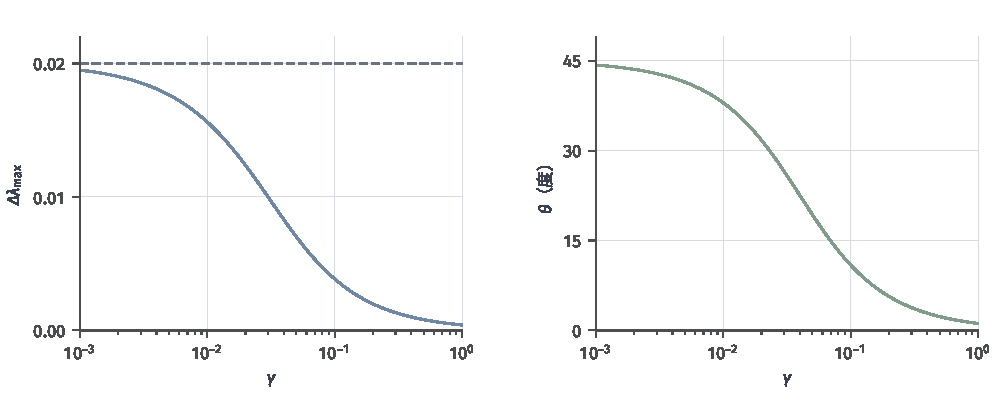
\includegraphics[width=169.0mm]{figures/01-mathematical-preliminaries-upper/02-linear-algebra-and-geometry/matplotlib/matrix-analysis-gap-direction/figure.pdf}
  \caption{同一对称扰动下，谱值稳定不等于方向稳定，固定$\epsilon=0.02$。
 左图为最大特征值增量
 $\Delta\lambda_{\max}=\sqrt{(\gamma/2)^2+0.02^2}-\gamma/2$，灰虚线为扰动范数$0.02$；
 右图为最大特征方向转角$\theta=\tfrac12\arctan(0.04/\gamma)$，角度用度表示。
 两图横轴均为原始谱隙$\gamma$，采用相同的对数刻度。
 所有数值均来自二阶特征方程的解析解。}
 \label{fig:matrix-analysis-gap-direction}
\end{figure*}

多个相邻特征值组成一簇时，应一次比较整个子空间。
设$1\leq r<d$，$\bm Q_r,\widetilde{\bm Q}_r$表示前$r$维特征子空间，
并有$\operatorname{sep}_r=\widetilde\lambda_r-\lambda_{r+1}>0$。
Davis--Kahan界在此单侧分离情形给出
\[
 \lVert\bm P-\widetilde{\bm P}\rVert_2
 \leq\frac{\lVert\bm E\rVert_2}{\operatorname{sep}_r}.
\]
为看清为何能控制整个块，取原补空间的正交基$\bm Q_\perp$，
令$\bm C=\bm Q_\perp^*\widetilde{\bm Q}_r$，
$\bm H=\bm Q_\perp^*\bm A\bm Q_\perp$、
$\bm K=\widetilde{\bm\Lambda}_r$、
$\bm D=\bm Q_\perp^*\bm E\widetilde{\bm Q}_r$。
投影后的特征方程为$\bm H\bm C-\bm C\bm K=-\bm D$。
由于$\lambda_{\max}(\bm H)\leq\lambda_{r+1}$、
$\lambda_{\min}(\bm K)=\widetilde\lambda_r$，其解为
\[
 \bm C=\int_0^\infty e^{t\bm H}\bm D e^{-t\bm K}\,\mathrm dt,
 \qquad
 \lVert\bm C\rVert_2
 \leq\int_0^\infty e^{-t\operatorname{sep}_r}\lVert\bm D\rVert_2\,\mathrm dt.
\]
对被积式求导可验证方程，指数衰减保证无穷端为零；
结合投影距离恒等式便得到上界。
原边界间隙$\delta=\lambda_r-\lambda_{r+1}$给出
$\operatorname{sep}_r\geq\delta-\lVert\bm E\rVert_2$。
对于中间谱簇，补谱分居两侧，应重新核对分离形式；
逐元素的Sylvester关系仍给出按最小谱距离控制的Frobenius界，
但不能不查条件就照搬上面的单侧谱范数常数。

簇内重数不妨碍比较整个块。例如$\operatorname{diag}(2,2,0)$的前二维基可任意旋转，
但投影恒为$\operatorname{diag}(1,1,0)$；$\lambda\bm I$中的单个方向则完全没有
可辨认性。PCA若在一组相等或接近的奇异值中间截断，边界方向同样敏感。
这不是某个特征向量算法的缺陷，而是目标没有把方向区分开。

自伴条件不可删去。若一般矩阵可对角化为$\bm V\bm\Lambda\bm V^{-1}$，
对扰动后任一特征值$\mu$，特征方程及对角逆范数给
$\min_i|\mu-\lambda_i|\leq
\lVert\bm V\rVert_2\lVert\bm V^{-1}\rVert_2\lVert\bm E\rVert_2$
（Bauer--Fike界）。当$\mu$本就是原特征值时结论直接成立；
否则由$(\bm\Lambda-\mu\bm I)\bm V^{-1}\bm w=-\bm V^{-1}\bm E\bm w$
求逆并约去$\lVert\bm w\rVert_2$即可。
不可对角化时甚至可能失去这种线性尺度，例如
$\left[\begin{smallmatrix}0&1\\0&0\end{smallmatrix}\right]$
在左下角加入$\epsilon>0$后，两个特征值变为$\pm\sqrt\epsilon$，
大于扰动范数$\epsilon$的量级。


矩形矩阵不能直接用普通特征谱，但可嵌入一个自伴矩阵。
定义对称扩张
\[
 \mathcal H(\bm A)=
 \begin{bmatrix}\bm0&\bm A\\\bm A^*&\bm0\end{bmatrix}.
\]
每个正奇异三元组给出扩张矩阵的特征向量
\[
 \frac1{\sqrt2}\begin{bmatrix}\bm u_i\\\bm v_i\end{bmatrix},
 \qquad
 \frac1{\sqrt2}\begin{bmatrix}\bm u_i\\-\bm v_i\end{bmatrix},
\]
对应特征值$\sigma_i$和$-\sigma_i$，剩余方向给零。
且$\lVert\mathcal H(\bm E)\rVert_2=\lVert\bm E\rVert_2$，
因为其平方为以$\bm E\bm E^*$、$\bm E^*\bm E$为对角块的矩阵。
Weyl界因此给出
\begin{equation}
 |\widetilde\sigma_i-\sigma_i|\leq\lVert\bm E\rVert_2,\qquad
 \widetilde{\bm A}=\bm A+\bm E.
 \label{eq:matrix-analysis-singular-value-perturbation}
\end{equation}
这不要求正奇异值之间有间隙。它也补齐前面的秩保持伪逆讨论：
若两矩阵秩同为$r>0$且$\lVert\bm E\rVert_2<\sigma_r(\bm A)$，
则$\sigma_r(\bm B)\geq\sigma_r(\bm A)-\lVert\bm E\rVert_2>0$，
可在式~\eqref{eq:ch06-pseudoinverse-fixed-rank-perturbation}取这一共同下界。
只有该不等式而没有同秩条件，仍不能排除原零奇异值变成新的微小正值。

左右方向则需要分别比较。设$1\leq k\leq\min(m,n)$，
$\bm U_k,\bm V_k$与$\widetilde{\bm U}_k,\widetilde{\bm V}_k$分别来自两矩阵的前$k$个
奇异方向，越过列表末端的奇异值按零计，并假设
$\operatorname{sep}_{\mathrm W}=\widetilde\sigma_k-\sigma_{k+1}>0$。
定义相对于原矩阵的两侧奇异方程残差
\[
 \bm R=\bm A\widetilde{\bm V}_k
        -\widetilde{\bm U}_k\widetilde{\bm\Sigma}_k,\qquad
 \bm S=\bm A^*\widetilde{\bm U}_k
        -\widetilde{\bm V}_k\widetilde{\bm\Sigma}_k.
\]
对于扰动矩阵的精确SVD，它们分别是
$-\bm E\widetilde{\bm V}_k$和$-\bm E^*\widetilde{\bm U}_k$。
Wedin正弦界的Frobenius版本为
\begin{equation}
 \left(
  \lVert\sin\bm\Theta(\bm U_k,\widetilde{\bm U}_k)\rVert_{\mathrm F}^2+
  \lVert\sin\bm\Theta(\bm V_k,\widetilde{\bm V}_k)\rVert_{\mathrm F}^2
 \right)^{1/2}
 \leq
 \frac{(\lVert\bm R\rVert_{\mathrm F}^2+\lVert\bm S\rVert_{\mathrm F}^2)^{1/2}}
      {\operatorname{sep}_{\mathrm W}}.
 \label{eq:matrix-analysis-singular-subspace-gap}
\end{equation}
为说明条件与常数，记左右补空间泄漏为
$\bm C=\bm U_\perp^*\widetilde{\bm U}_k$、
$\bm D=\bm V_\perp^*\widetilde{\bm V}_k$。
对原来未保留的一对奇异方向$j>k$和目标列$i\leq k$，投影残差得到
\[
 \begin{bmatrix}-\widetilde\sigma_i&\sigma_j\\
                 \sigma_j&-\widetilde\sigma_i\end{bmatrix}
 \begin{bmatrix}C_{j,i}\\D_{j,i}\end{bmatrix}
 =\begin{bmatrix}(\bm U_\perp^*\bm R)_{j,i}\\
                  (\bm V_\perp^*\bm S)_{j,i}\end{bmatrix},
\]
其中$j$在补空间矩阵中按相应行索引理解。
该二阶块的最小奇异值为$\widetilde\sigma_i-\sigma_j
\geq\operatorname{sep}_{\mathrm W}$。
矩形多出来的未配对零方向只需除以$\widetilde\sigma_i$，也不小于同一分离量。
各项平方求和，再用投影不增加Frobenius范数及
$\lVert\bm C\rVert_{\mathrm F}=\lVert\sin\bm\Theta_U\rVert_{\mathrm F}$，
便得到式~\eqref{eq:matrix-analysis-singular-subspace-gap}\scite{math-golub2013matrix}。

因此两侧角度的总量至多为
$\sqrt{2k}\lVert\bm E\rVert_2/\operatorname{sep}_{\mathrm W}$；
保留残差形式往往比这个粗界更有信息，也能评价近似算出的奇异向量。
前$k$个奇异值内部允许重复，控制整个块只需边界分离；
要辨认其中一个向量，还需与两侧相邻值分离，并排除零值的自由延拓。
原边界间隙$\delta=\sigma_k-\sigma_{k+1}$给
$\operatorname{sep}_{\mathrm W}\geq\delta-\lVert\bm E\rVert_2$。
没有可靠边界间隙时，最优低秩误差仍可稳定，却不能把算法返回的某组压缩方向
当作唯一的数据结构。PCA与低秩近似必须分别报告误差尺度和方向可辨认性。

\subsection{矩阵函数的稳定性}
\label{sec:linear-algebra-matrix-function-stability}
\label{sec:ch06-matrix-function-stability}


幂、指数和平方根将一个矩阵变成另一个矩阵。矩阵输入的扰动会插入乘积的不同位置，
这些位置一般不能合并。先对固定整数$k\geq1$展开，得到
\[
 (\bm A+\bm E)^k-\bm A^k
 =\sum_{j=0}^{k-1}\bm A^{k-1-j}\bm E\bm A^j+O(\lVert\bm E\rVert^2).
\]
例如平方的一阶项是$\bm A\bm E+\bm E\bm A$，不总是$2\bm A\bm E$。
对有限扰动还有精确的望远镜恒等式
\[
 (\bm A+\bm E)^k-\bm A^k
 =\sum_{j=0}^{k-1}(\bm A+\bm E)^{k-1-j}\bm E\bm A^j.
\]
因此其范数不超过$kM^{k-1}\lVert\bm E\rVert$，
$M=\max(\lVert\bm A+\bm E\rVert,\lVert\bm A\rVert)$。
此界对固定$k$成立，随$k$可能快速增大；
单次变换接近并不保证所有迭代次数的结果都同样接近。

沿用第~\ref{chap:mathematical-analysis}章的全微分，把矩阵看成有限坐标对象。
若$f$在$\bm A$的一个开邻域中有定义，且存在对$\bm E$线性的映射$L_f$使
\begin{equation}
 f(\bm A+\bm E)-f(\bm A)
 =L_f(\bm A,\bm E)+o(\lVert\bm E\rVert),
 \label{eq:matrix-analysis-frechet-derivative}
\end{equation}
则$L_f$称为相应\term{Fréchet导数}（Fréchet derivative）。
讨论实自伴矩阵时，开邻域指自伴矩阵空间中的开集，
不是默许任意非自伴扰动仍使用相同实谱定义。
上述幂展开给出多项式函数的导数；高阶余项的常数依赖$\bm A$和固定次数，
不能在次数增大时无条件保持。

自伴谱使一般函数的一阶变化可按坐标计算。
设$\bm A=\bm Q\operatorname{diag}(\lambda_i)\bm Q^*$，
$f$在包含该谱的实开区间上连续可微。定义一阶差商矩阵
\[
 F^{[1]}_{i,j}=
 \begin{cases}
  \dfrac{f(\lambda_i)-f(\lambda_j)}{\lambda_i-\lambda_j},
    &\lambda_i\neq\lambda_j,\\[5pt]
  f'(\lambda_i),&\lambda_i=\lambda_j.
 \end{cases}
\]
对自伴扰动有
\begin{equation}
 L_f(\bm A,\bm E)
 =\bm Q\bigl(\bm F^{[1]}\odot(\bm Q^*\bm E\bm Q)\bigr)\bm Q^*.
 \label{eq:matrix-analysis-frechet-divided-difference}
\end{equation}
对单项式$z^k$，把上一段的各插入项写到特征坐标中，其$(i,j)$元素的系数是
$\sum_{\ell=0}^{k-1}\lambda_i^{k-1-\ell}\lambda_j^\ell$，
不同根时等于差商，相同根时等于$k\lambda_i^{k-1}$，故多项式情况已证。
对一般$C^1$函数，取多项式$p$在有限个不同谱点上同时匹配$f$和$f'$。
这样的多项式为何存在，可以用已知的维数原理说明。设不同谱点共$s$个，
将次数小于$2s$的多项式映到这$s$点的函数值与一阶导数，得到一个线性映射。
若所有读数都为零，多项式在每个谱点都有二重零点，即能被各
$(z-\lambda_i)^2$的乘积整除；次数限制使它只能为零。
这个映射的定义域和值域同为$2s$维，单射便是满射，因而可以匹配任意给定的
$2s$个读数，包括$f$和$f'$在谱点上的值。
余函数$g=f-p$在每个谱点均有$g=g'=0$，故附近
$g(\lambda_i+h)=o(|h|)$。由Weyl界，$\bm A+\bm E$的每个特征值距原谱不超过
$\lVert\bm E\rVert_2$，于是
$\lVert g(\bm A+\bm E)\rVert_2=o(\lVert\bm E\rVert_2)$，
且$g(\bm A)=0$。所以多项式的导数表达也给$f$的导数，证明余项条件。

对角项由标量导数控制，非对角项由不同谱点的差商控制。
当$\bm A\bm E=\bm E\bm A$时，扰动在不同特征值块之间没有耦合，
可化为$L_f=f'(\bm A)\bm E$；
交换性是充分条件，不是必要条件，例如仿射$f$即使不交换也满足这个形式。
在Frobenius范数下，差商表达还直接给
$\lVert L_f(\bm A,\bm E)\rVert_{\mathrm F}
\leq\max_{i,j}|F^{[1]}_{i,j}|\lVert\bm E\rVert_{\mathrm F}$，
这提供当前函数任务的局部绝对敏感性。

指数对任何方阵均有定义。令$\bm B=\bm A+\bm E$，
对$e^{(1-s)\bm B}e^{s\bm A}$关于$s$求导并积分，得到
\[
 e^{\bm A+\bm E}-e^{\bm A}
 =\int_0^1e^{(1-s)(\bm A+\bm E)}\bm E e^{s\bm A}\,\mathrm ds.
\]
其中保留了$\bm E$两侧的次序。在有界邻域内，把第一指数中的$\bm E$去掉只改变
$O(\lVert\bm E\rVert^2)$，因此
\begin{equation}
 L_{\exp}(\bm A,\bm E)
 =\int_0^1e^{(1-s)\bm A}\bm E e^{s\bm A}\,\mathrm ds.
 \label{eq:matrix-analysis-exponential-frechet-derivative}
\end{equation}
交换时可合成$e^{\bm A}\bm E$；一般情形不行。
例如$\bm A=\operatorname{diag}(0,\log2)$，
$\bm E=\left[\begin{smallmatrix}0&1\\1&0\end{smallmatrix}\right]$时，
导数的两个非对角元均为$1/\log2$，而$e^{\bm A}\bm E$的两个非对角元分别为$1$和$2$。
有限差的粗界为
$\lVert e^{\bm A+\bm E}-e^{\bm A}\rVert
\leq e^{\max(\lVert\bm A+\bm E\rVert,\lVert\bm A\rVert)}\lVert\bm E\rVert$；
非正规结构或更具体范数可能需要更细评价。

平方根的定义域更窄。设$\bm A\succ0$，$\bm S=\bm A^{1/2}\succ0$，
只考虑保持正定的自伴扰动。对$\bm S^2=\bm A$求一阶变化，
$\bm Z=L_{\sqrt{\cdot}}(\bm A,\bm E)$必须满足
\[
 \bm S\bm Z+\bm Z\bm S=\bm E.
\]
这是前面定义并分析过的Sylvester方程，而不是$2\bm S\bm Z=\bm E$。
$\bm S$的特征值$s_i>0$保证全部$s_i+s_j>0$，
故解唯一，且在特征基中
\[
 (\bm Q^*\bm Z\bm Q)_{i,j}
 =\frac{(\bm Q^*\bm E\bm Q)_{i,j}}{s_i+s_j}.
\]
这一表达与$f(z)=\sqrt z$的差商完全相同，因此确实给出微分，而不只是必要方程。
它还给Frobenius界
$\lVert\bm Z\rVert_{\mathrm F}
\leq\lVert\bm E\rVert_{\mathrm F}/(2\sqrt{\lambda_{\min}(\bm A)})$。
例如$\bm A=\operatorname{diag}(1,4)$，上述非对角扰动给
$Z_{1,2}=Z_{2,1}=1/3$；直接写成
$\tfrac12\bm A^{-1/2}\bm E$会得到$1/2$和$1/4$，不仅数值错，也失去自伴性。

若$\bm A$只有半正定，在零谱方向上$\sqrt\epsilon/\epsilon=1/\sqrt\epsilon$无界，
不能沿用正定邻域的可微性或含$s_i+s_j$的逆。
可逆矩阵的微分
$D(\bm A^{-1})[\bm E]=-\bm A^{-1}\bm E\bm A^{-1}$，
以及正定域上标量函数
$D(\log\det\bm A)[\bm E]=\operatorname{tr}(\bm A^{-1}\bm E)$，
回用第~\ref{chap:mathematical-analysis}章的推导；
前者的有限扰动在本章已经分析，后者的标量输出不等于矩阵$\log\bm A$的导数。

函数计算仍要评价算法，而不止评价导数。
例如程序返回自伴正定候选$\widehat{\bm S}$，其平方根方程残差为
$\bm R=\widehat{\bm S}^{\,2}-\bm A$。
令$\bm D=\widehat{\bm S}-\bm S$，则精确有
$\widehat{\bm S}\bm D+\bm D\bm S=\bm R$。
正定性与Sylvester积分表示给出，在谱范数或Frobenius范数下，
\[
 \lVert\widehat{\bm S}-\bm S\rVert
 \leq\frac{\lVert\bm R\rVert}
 {\lambda_{\min}(\widehat{\bm S})+\sqrt{\lambda_{\min}(\bm A)}}.
\]
同时$\widehat{\bm S}$是邻近正定输入$\bm A+\bm R$的精确正定平方根，
所以残差也给后向误差解释。若不检查正定分支，$\widehat{\bm S}=-\bm S$
有零残差却不是所求平方根；若分母很小，小残差仍可能对应较大前向误差。

幂的快速平方、指数的缩放与平方以及Schur形式上的函数计算都有各自的舍入传播。
应把返回值与同一输入的精确函数值比较，并检查方法声明的前向或后向界；
一个解析恒等式并不自动证明实现稳定。至此，表示、求解、迭代和压缩都回到了相同的
检验原则：先说明目标对象及条件，再给误差尺度和可计算的证据。

\section{本章小结}
\label{sec:linear-algebra-summary}
\label{sec:matrix-analysis-summary}


近共线设计矩阵把本章的几种问题串联起来。对象所在的空间决定什么能够线性组合，
基决定怎样记坐标，内积和范数决定怎样比较误差；两列几乎同向时，同一个输出可由
两个很大的相消系数表示。坐标很大不等于对象很大，换坐标也不等于施加了一个新变换。
矩阵通过基像记录变换，加法、复合、分块和索引缩并则组织其运算；
固定权重的线性读取不能替代对完整注意力或其他输入依赖操作的分析。

反求输入先问输出是否可达。不可达时，投影给最近输出；输入不唯一时，
零空间正交补再给最小范数选择，二者共同确定伪逆。
LU、QR、Cholesky与迭代法落实这些任务，但它们使用的结构不同。
零初始化梯度迭代能选出最小范数解，是因为更新留在行空间，
并不是所有下降算法都隐含同一种范数偏好。

反复作用要求同一个方阵。特征方向足够时，幂化成各尺度的幂；
方向不足时，Jordan幂零部分带来多项式因子。
二维迭代例说明长期衰减与短时放大可以并存：
谱半径控制固定矩阵的长期衰减，非正交方向间的相消影响有限步长度。
指数、平方根和对数还有各自定义域，非交换微分必须保留左右作用的次序。

压缩关注的是保留多少输入输出方向。SVD先给精确的正交配对，
截断才在秩预算下给最优误差；反过来，最大尾奇异值或尾部平方能量确定误差阈值所需
的最小秩。PCA是中心化有限数据的平方重构实例，核范数惩罚会改变目标，
稳定秩等辅助尺度则不能替代具体误差约束下的最优整数秩。

答案存在、表示唯一、近似最优、方向可辨认和计算可靠是不同保证。
近共线性使小奇异方向在反求中放大，即使训练拟合稳定，系数与外推仍可能敏感；
截断和岭收缩降低敏感性，同时舍弃或削弱信息。
谱值变化小也不保证方向稳定，子空间需有相对于扰动的可靠分离。
后向稳定算法只引入小的等效输入变化，能否得到小前向误差仍由问题条件决定。
保留这些区别，才能在后续概率、信号和动态问题中正确使用同一套矩阵工具。
第~\ref{chap:differential-geometry-and-symmetry}章进一步研究局部坐标、切空间、
度量与对称性，线性变换将在那里成为描述弯曲空间局部行为的工具。

\chapter{非线性空间与流形}
\label{chap:differential-geometry-and-symmetry}

上一章在固定向量空间中区分了对象、坐标与线性变换。现在把可选对象限制在一个圆上：
两个圆上点的平均值通常不在圆上，沿切线走有限一步也会离开圆。怎样记录位置、选择
可行的变化方向，并比较两点之间的路程？这些问题不能只靠换一组基解决，因为限制来自
可行集合本身。即使每个小邻域都近似平直，局部记录也未必能拼成一组全局坐标。

本章以平面中的弯曲点带连接这些问题。连续带、它的中心线和带噪观测是不同对象：
带有纵横两个自由度，中心线只有一个；测量误差则描述观测怎样偏离潜在点，不自动增加
潜在空间的自由度。有限点间距离可以帮助重构坐标，对称变换说明哪些记录代表等价输入，
邻域关系则补充连通与环的信息。它们各自回答一种表示问题，不是四种互斥的空间类型。

在确定光滑流形这一连续模型以后，局部线性化给出可行速度，度量给速度规定长度，
路径积分再定义路程和距离。比较不同位置的方向还需要额外的搬运规则，由此才能讨论
局部直行与曲率。本章的优化未知量是流形中的点；定义在整个流形上的函数与场，留给下一章研究。以下主要使用基础分析、线性代数和前文优化知识；有限距离模型与
组合拓扑模型本身不被假定为光滑流形。

\section{元素与表示}
\label{sec:geometry-nonlinear-representations}

点带上的一个潜在位置可以由$(s,u)$记录，测量得到的环境坐标则可能带误差。
这两种记录不能直接互换：前者需要先确定连续可行集合，后者还包含测量过程。
下面先界定对象，再建立局部坐标与重叠区域中的坐标转换。

\subsection{对象与空间的界定}
\label{sec:geometry-objects}

圆上两个点的和通常不在圆上，所以可行位置不能直接组成上一章的向量空间。
本章改用局部有限自由度描述可行集合。建模时要分别指定连续集合、容纳它的环境空间和有限观测：
集合限制哪些位置可行，环境坐标记录位置，观测则提供关于未知位置的信息。
贯穿本章的\term{弯曲点带}取为
\begin{equation}
 \Phi(s,u)=
 \begin{bmatrix}
 (R+u)\cos(s/R)\\(R+u)\sin(s/R)
 \end{bmatrix},
 \qquad s\in I,\quad |u|<w<R,
 \label{eq:geometry-curved-strip-parameterization}
\end{equation}
其中$R>0$，$I=(s_-,s_+)$的长度小于$2\pi R$，防止绕回后重复。
$s$沿中心线定位，$u$记录横向偏移。定义
\[
 \mathcal M_{\mathrm{strip}}=\{\Phi(s,u):s\in I,\ |u|<w\},
 \qquad \mathcal C=\{\Phi(s,0):s\in I\}.
\]
前者是二维开带，后者是一维中心线，二者均不包括端点。
连续双射且逆映射也连续，称为同胚（homeomorphism）；它保留连续性关系。
开带与开矩形同胚，中心线与开区间同胚。
其参数化是否满秩将在计算局部方向时直接核对。

从这个连续模型采样时，\term{潜在点}（latent point）
$\bm p_i=\Phi(s_i,u_i)$指误差发生前的真实位置，
$\bm x_i=\bm p_i+\bm\epsilon_i$才是观测。二维开带是$\mathbb R^2$的开集，
故内部点足够小的扰动仍在带内，但不等于原潜在点；无噪声界则不保证仍在带内。
若选择的潜在对象是一维中心线，就要求$u_i=0$，把横向偏离归入观测误差。
一般扰动会将观测推出中心线，不能一面声称潜在对象一维，一面又把误差当作第二个
内在坐标。有限点云宽度很小也不足以决定这项建模选择。

\subsection{对象的局部坐标表示}
\label{sec:geometry-manifold-coordinates}
\label{sec:geometry-local-coordinate-representation}

\label{sec:geometry-local-charts}

在圆的一小段上，一个角度便能定位一个点；绕完整圆却必然遇到角度断点或重复表示。
\term{流形}（manifold）把这两件事分开：它要求每个点附近像某个欧氏开集，
并不要求整个对象是一张欧氏坐标表。本章先讨论欧氏空间中的光滑嵌入流形；
光滑指各阶导数连续，微分同胚指映射及其逆都光滑\scite{math-lee2013smooth}。

\begin{definition}[光滑嵌入流形]
\label{def:geometry-embedded-manifold}
设$0\leq d\leq D$。集合$\mathcal M\subseteq\mathbb R^D$称为$d$维光滑嵌入流形，
若每个$\bm p\in\mathcal M$都有包含它的环境开集$O$和欧氏开集之间的微分同胚
$\Psi:O\to\Psi(O)\subseteq\mathbb R^D$，满足
\[
 \Psi(\mathcal M\cap O)
 =\Psi(O)\cap(\mathbb R^d\times\{\bm0_{D-d}\}).
\]
\end{definition}
这个条件用已经学过的欧氏光滑映射把对象局部拉直，因而没有用“流形上的光滑逆”
循环定义流形。前$d$个坐标描述局部自由度，$D$只是容纳对象的环境维数。

令$U=\{\bm z:(\bm z,\bm0_{D-d})\in\Psi(O)\}$，则
$\varphi(\bm z)=\Psi^{-1}(\bm z,\bm0_{D-d})$从开集$U\subseteq\mathbb R^d$
参数化$\mathcal M\cap O$，且Jacobian满列秩。一般局部参数化还须在其像上具有
连续逆；仅仅满秩并不能排除全局绕回或自交。参数化的方向是“坐标到点”，
读取一个点的位置则要使用反向映射。


参数化的逆$\chi=\varphi^{-1}:\mathcal M\cap O\to U$称为
\term{坐标图}（chart）。覆盖整个流形的一组坐标图称为图册（atlas）；
“局部像$\mathbb R^d$”指有这种局部记录方式，不是说流形在环境中必须平直。

\subsection{坐标的转换}
\label{sec:geometry-coordinate-conversions}

同一点可能由两张图记录。要让这两份记录兼容，需要明确坐标之间的转换。
\begin{definition}[坐标过渡]
\label{def:geometry-chart-transition}
两张图的覆盖区域相交时，$\chi_2\circ\chi_1^{-1}$把第一组坐标换成第二组坐标，
称为\term{坐标过渡}（coordinate transition），定义在交集的第一组坐标像上。
\end{definition}
坐标过渡及其逆都光滑，因此在重叠区域中换图不改变光滑性。

单位圆的参数化$\varphi(\theta)=(\cos\theta,\sin\theta)^\top$限制到
$(-\pi,\pi)$时漏掉$(-1,0)^\top$，限制到$(0,2\pi)$时漏掉$(1,0)^\top$。
两张图合起来覆盖圆，交叠处的过渡是$\theta$或$\theta+2\pi$。
断点移动的是坐标，不是圆被切断了。
完整圆是紧集，它在连续映射下的像仍紧；非空的一维欧氏开集却不紧，
所以圆不可能与这种开集同胚，也不能靠一张无重复的实数坐标图覆盖。
它局部一维，却至少需要二维环境才能
无自交地全局嵌入；局部维数、环境维数与最小全局嵌入维数由不同条件决定。图~\ref{fig:geometry-circle-chart-transition}给出同一圆上两个点在两张图中的记录。

\begin{figure}[htbp]
  \centering
  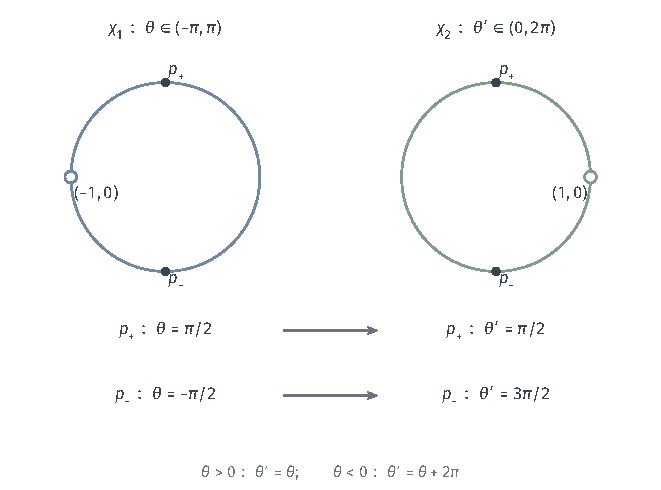
\includegraphics[width=112.0mm]{figures/01-mathematical-preliminaries-upper/02-linear-algebra-and-geometry/tikz/geometry-circle-chart-transition/figure.pdf}
  \caption{单位圆的两张坐标图。空心点分别是各图漏掉的$(-1,0)^\top$与$(1,0)^\top$，两图合起来覆盖完整圆。两图中的$p_+$相互对应，$p_-$也相互对应；每对标记记录同一个几何点。上半圆过渡保持角度，下半圆过渡加$2\pi$。图下方列出两个交叠分支的转换，不把坐标断点理解为圆被切断。}
  \label{fig:geometry-circle-chart-transition}
\end{figure}




同一个点在两张图中的坐标不同，过渡映射必须把旧记录送到新记录。
三张图共同覆盖时，$\chi_3\circ\chi_1^{-1}
=(\chi_3\circ\chi_2^{-1})\circ(\chi_2\circ\chi_1^{-1})$，
等式只在各步都有定义的重叠区域使用。与线性换基相同，中间记录消去；
不同之处在于过渡通常非线性且只在局部有效。

\section{关系与结构}
\label{sec:geometry-relations}

两条圆弧在小邻域中都可以用一个坐标记录，却可能属于不同的连通分支；
同一圆上的两点也有不同切线。局部坐标之外，还需建立邻域、切向与距离关系，
分别描述连续连接、可行速度与路线代价。若任务要忽略旋转或重编号，再以等价关系规定这种忽略。

\subsection{对象的邻域关系}
\label{sec:geometry-neighborhood-relations}
\label{sec:geometry-local-relations-topology}

\label{sec:geometry-neighborhood-topology}

在嵌入模型中，$\mathcal M\cap O$（$O$为环境开集）给出相对开集。
包含一个含有该点的相对开集的集合，称为该点的邻域。开集的任意并、有限交仍开，
它们决定连续映射、连通与局部记录所需的关系。
两条互不相交的开圆弧和一条完整圆，每个点附近都像一维开区间，
整体却分别有两个连通分支和一个不可在圆内缩到点的环。
\term{拓扑}（topology）在这里研究连续连接与孔洞等结构，
不要求保持长度和角度。把开点带连续拉直可以保留连接关系，
把两端粘合却改变了对象。局部自由度不能回答这种整体问题。

有限欧氏点集继承的拓扑是离散的；要从样本推测连续形状，必须额外选择哪些邻域算相连。
而一圈边是否被填满又不是成对连边能够决定的。为使$k+1$个顶点确实张成$k$维形状，
要求以一个顶点$\bm v_0$为基点时，差向量
$\bm v_1-\bm v_0,\ldots,\bm v_k-\bm v_0$线性无关；
这称为顶点的仿射独立（affine independence），三个顶点时就是不共线。
$k$维\term{单纯形}（simplex）在几何上是这些顶点的凸包，在组合表示中只记录顶点集合。
点、线段、填充三角形分别是零、一、二维单纯形。
仿射独立保证几何维数；组合形式则用于指定哪些高阶面存在。

\begin{definition}[抽象单纯复形]
\label{def:geometry-simplicial-complex}
有限顶点集上的\term{抽象单纯复形}（abstract simplicial complex）
$\mathcal K$是一族非空顶点子集，满足向下封闭：
\begin{equation}
 \sigma\in\mathcal K,\quad\varnothing\neq\tau\subseteq\sigma
 \quad\Longrightarrow\quad\tau\in\mathcal K.
 \label{eq:geometry-simplicial-complex-closure}
\end{equation}
含$k+1$个顶点的元素称为$k$维单纯形。
\end{definition}
加入三角面必须连同它的三条边和三个顶点一起加入，反之不成立。
这使复形能够区分“围出一圈”和“这一圈已由一个面填充”。


为计算未被填充的环，需要把端点抵消与高阶填充分别记录。
选定顶点次序后，以$[v_0,\ldots,v_k]$表示有向单纯形，交换两顶点使符号反转。
有向$k$维单纯形的实系数线性组合称为$k$维链，
组成向量空间$C_k(\mathcal K;\mathbb R)$。边界算子读取每个面的有向边缘：
\begin{equation}
 \partial_k[v_0,\ldots,v_k]
 =\sum_{i=0}^k(-1)^i[v_0,\ldots,\widehat{v_i},\ldots,v_k],
 \qquad k\geq1,
 \label{eq:geometry-simplicial-boundary}
\end{equation}
尖帽表示删去该顶点，算子线性延伸到全部链。
本章采用非约化同调，约定$C_{-1}=\{0\}$、$\partial_0=0$。
例如$\partial_1[1,2]=[2]-[1]$，端点的正负表示方向。

\begin{lemma}[边界的边界为零]
\label{lem:geometry-boundary-squared-zero}
上述算子满足
\begin{equation}
 \partial_{k-1}\partial_k=0,\qquad k\geq1.
 \label{eq:geometry-boundary-squared-zero}
\end{equation}
\end{lemma}
\begin{proof}
$k=1$时由$\partial_0=0$成立。对$k\geq2$，固定$i<j$，
两次删除$v_i,v_j$后得到相同的$(k-2)$维面。
先删$i$再删原来的$j$，系数为$(-1)^i(-1)^{j-1}$；
先删$j$再删$i$，系数为$(-1)^j(-1)^i$，两者相反。
所有项都按这样的顶点对成对抵消，因此结论对基单纯形成立；
由线性性，对全部链成立。
\end{proof}

边界必定闭合，但闭合的圈未必由复形中的某个面填充。
这正好可以用上一章的核、像与商空间表达。
\begin{definition}[闭链、边界与同调空间]
\label{def:geometry-homology-space}
满足$\partial_kc=0$的链称为\term{闭链}（cycle），
能写成$c=\partial_{k+1}b$的链称为\term{边界}（boundary）。
由$\partial_k\partial_{k+1}=0$，有
$\operatorname{im}\partial_{k+1}\subseteq\ker\partial_k$。
实系数\term{同调空间}（homology space）及其维数定义为
\[
 H_k(\mathcal K;\mathbb R)=\ker\partial_k/\operatorname{im}\partial_{k+1},
 \qquad \beta_k=\dim H_k(\mathcal K;\mathbb R).
\]
$\beta_k$称为第$k$个\term{Betti数}（Betti number）。
\end{definition}
商空间沿用定义~\ref{def:linear-algebra-quotient-space}：
两个闭链相差一个边界时被视为同类。因而$H_k$保留的不是全部闭链，
而是无法用已有高阶填充消去的部分；$\beta_0$计算连通分支，
$\beta_1$计算实系数意义下独立的一维环。

取
$\mathcal K_{\mathrm{loop}}
=\{\{1\},\{2\},\{3\},\{1,2\},\{2,3\},\{1,3\}\}$。
链$c=[1,2]+[2,3]-[1,3]$的端点逐一抵消，故$\partial_1c=0$。
$\partial_1$的秩为$2$，一维闭链空间维数为$3-2=1$，
而没有二维面，故$\beta_1=1$、$\beta_0=3-2=1$。
加入$[1,2,3]$后，$c=\partial_2[1,2,3]$成为边界，$\beta_1$降为$0$；
$\partial_1$不变，所以$\beta_0$仍为$1$。
图~\ref{fig:geometry-cycle-filled-simplex}只改变面集合，顶点与边保持相同。
\begin{figure}[htbp]
  \centering
  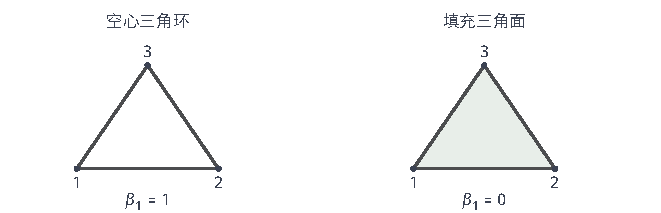
\includegraphics[width=112.0mm]{figures/01-mathematical-preliminaries-upper/02-linear-algebra-and-geometry/tikz/geometry-cycle-filled-simplex/figure.pdf}
  \caption{一圈边是否已填充，取决于高阶面而非边图。左侧闭链
 $c=[1,2]+[2,3]-[1,3]$不是边界；右侧加入$[1,2,3]$后有
 $c=\partial_2[1,2,3]$。两者$\beta_0=1$，$\beta_1$分别为$1$与$0$。
 图为组合教学示例，不代表某个观测点云的真实拓扑。}
 \label{fig:geometry-cycle-filled-simplex}
\end{figure}


若$N_k$是$k$维单纯形数，Euler示性数
$\chi=\sum_k(-1)^kN_k$是更粗的摘要：空心三角形为$3-3=0$，
填充三角形为$3-3+1=1$。由秩--零度关系
$N_k=\beta_k+\operatorname{rank}\partial_k+\operatorname{rank}\partial_{k+1}$，
交替求和后中间秩抵消，也得到$\chi=\sum_k(-1)^k\beta_k$。
不同Betti数组甚至不同拓扑都可能有同一个$\chi$，一个标量不足以代替分别分析。

\subsection{对象的位置与方向关系}
\label{sec:geometry-position-direction-relations}
\label{sec:geometry-manifold-local-linearization}
\label{sec:geometry-analytic-local-linearization}

从$\bm p=\varphi(\bm z)$出发，坐标变化$\bm v$经Jacobian
$\bm J_\varphi(\bm z)$映为环境空间中的瞬时速度。
\term{切空间}（tangent space）收集所有这样的可行速度；
它描述一阶方向，并不是可行集合本身的一小块。

\begin{definition}[嵌入流形的切空间]
\label{def:geometry-tangent-space}
设$\varphi:U\subseteq\mathbb R^d\to\mathcal M\subseteq\mathbb R^D$
是局部参数化，$\bm p=\varphi(\bm z)$。定义
\begin{equation}
 T_{\bm p}\mathcal M
 =\{\bm J_\varphi(\bm z)\bm v:\bm v\in\mathbb R^d\}.
 \label{eq:geometry-tangent-space-chart}
\end{equation}
\end{definition}
Jacobian列满秩保证这是$d$维向量空间，其原点是零速度。
画在$\bm p$旁边的仿射切平面则是$\bm p+T_{\bm p}\mathcal M$；
点的位置与速度向量的零点不能混为一谈。

\begin{lemma}[曲线速度与坐标刻画相容]
\label{lem:geometry-tangent-curves}
$T_{\bm p}\mathcal M$恰是全部光滑曲线
$\gamma:(-\epsilon,\epsilon)\to\mathcal M$、$\gamma(0)=\bm p$
的速度$\gamma'(0)$组成的集合，并且与局部坐标选择无关。
\end{lemma}
\begin{proof}
在足够小的参数区间内，曲线落入当前坐标图，写成
$\gamma(t)=\varphi(\bm z(t))$。链式法则给出
$\gamma'(0)=\bm J_\varphi(\bm z)\bm z'(0)$，故每个曲线速度都属于所定义的空间。
反过来，任意$\bm v\in\mathbb R^d$给出曲线
$t\mapsto\varphi(\bm z+t\bm v)$；因为$U$开，足够小的$t$仍在定义域内，
其初速度为$\bm J_\varphi(\bm z)\bm v$。

若另一参数化满足$\widetilde\varphi=\varphi\circ\psi$，
坐标过渡$\psi$的Jacobian可逆，且
$\bm J_{\widetilde\varphi}=\bm J_\varphi\bm J_\psi$。
右乘可逆矩阵不改变值域，两张图因而给出同一切空间。
\end{proof}

在点带中直接求导，可核对两个自由度：
\begin{align}
 \frac{\partial\Phi}{\partial s}
 &=\left(1+\frac uR\right)
   \begin{bmatrix}-\sin(s/R)\\\cos(s/R)\end{bmatrix},
 \label{eq:geometry-strip-s-tangent}\\
 \frac{\partial\Phi}{\partial u}
 &=\begin{bmatrix}\cos(s/R)\\\sin(s/R)\end{bmatrix}.
 \label{eq:geometry-strip-u-tangent}
\end{align}
因$|u|<w<R$，第一列不为零，两列正交且线性无关；
开带的切空间是整个$\mathbb R^2$。中心线则只允许$u=0$，
\[
 T_{\Phi(s,0)}\mathcal C
 =\operatorname{span}\{(-\sin(s/R),\cos(s/R))^\top\}.
\]
径向方向对开带可行，对中心线不可行。中心线的切线随位置转动，
没有一条固定线性子空间等于各处的切空间。

图~\ref{fig:geometry-strip-tangent-coordinates}上半部把切向速度画在点旁，
下半部比较同一坐标增量对应的实际弧长。方向数目决定局部维数，
坐标增量怎样换算为长度则留待度量处理。
\begin{figure}[htbp]
  \centering
  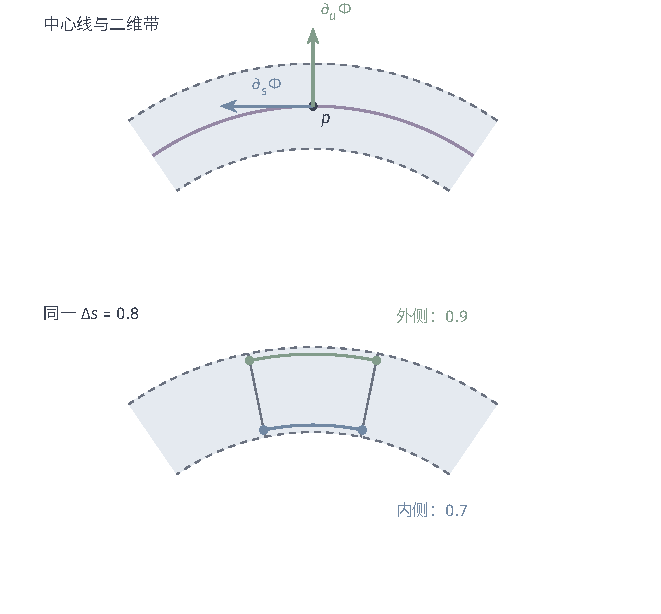
\includegraphics[width=112.0mm]{figures/01-mathematical-preliminaries-upper/02-linear-algebra-and-geometry/tikz/geometry-strip-tangent-coordinates/figure.pdf}
  \caption{开带与中心线的局部方向不同。取$R=2$、$w=0.3$。
 上图的两个参数方向属于二维开带，仅以中心线为对象时，径向方向不属于其切空间；
 箭头平移到$\bm p$只是画法。下图取$u=-0.25,0.25$，同一$\Delta s=0.8$
 对应圆弧长度$0.7,0.9$。灰虚线为不纳入开带的边界，两图等比例绘制，均为解析教学示例。}
 \label{fig:geometry-strip-tangent-coordinates}
\end{figure}


若流形由约束$F(\bm x)=\bm0$给出，其中
$F:\mathbb R^D\to\mathbb R^{D-d}$在$\bm p$附近光滑且
$\bm J_F(\bm p)$行满秩，就能选出$D-d$列组成可逆方阵。
重排坐标后，定理~\ref{thm:analysis-implicit-function}把这$D-d$个变量
解为其余$d$个变量的光滑函数，后者便给出局部参数化。
对约束内曲线求导得$\bm J_F(\bm p)\gamma'(0)=\bm0$；
所以切空间包含于该矩阵的核。参数化给出$d$维切空间，
秩--零度关系又说明核为$d$维，故$T_{\bm p}\mathcal M=\ker\bm J_F(\bm p)$。
满秩条件不能省略：$F(x,y)=x^2+y^2$在原点导数为零，
核是整个平面，但零水平集只有一个点，真实可行速度只有零向量。

\subsection{对象的距离关系}
\label{sec:geometry-metric-length-distance}
\label{sec:geometry-metric-path-geodesic}
\label{sec:geometry-same-point-metric}

\label{sec:geometry-riemannian-metric}
\label{sec:geometry-path-speed-length}
\label{sec:geometry-endpoint-distance}
\label{sec:geometry-continuous-geodesic-distance}

切空间说明方向可不可行，却没有规定一单位坐标变化有多长。
点带外侧与内侧相同的$\mathrm ds$对应不同弧长，因而内积必须按位置指定。
\term{Riemann度量}（Riemannian metric）为每个切空间提供这种长度与夹角规则。

在局部参数化$\varphi$中，把坐标记为$(z^1,\ldots,z^d)$；
上标在这里是坐标编号。相应坐标切基为
$\partial_i=\partial\varphi/\partial z^i$。

\begin{definition}[Riemann度量]
\label{def:geometry-riemannian-metric}
光滑流形$\mathcal M$上的Riemann度量$g$为每个$\bm p$指定内积
$g_{\bm p}:T_{\bm p}\mathcal M\times T_{\bm p}\mathcal M\to\mathbb R$，
且在任一光滑坐标切基$\partial_i$中，矩阵
$\bm G(\bm z)=[g_{i,j}(\bm z)]$、$g_{i,j}=g(\partial_i,\partial_j)$
的条目光滑。每个$\bm G$都对称正定。
\end{definition}
对同点切向量$\bm v,\bm w$，长度为
$\lVert\bm v\rVert_g=\sqrt{g_{\bm p}(\bm v,\bm v)}$；
非零时夹角满足
$\cos\vartheta=g_{\bm p}(\bm v,\bm w)/
(\lVert\bm v\rVert_g\lVert\bm w\rVert_g)$。
若它们的坐标分量为$\bm a,\bm b$，内积是$\bm a^\top\bm G\bm b$。
$\bm G$既不是样本协方差，也不必是全空间共享的常矩阵。

嵌入流形可以限制环境欧氏内积，得到诱导度量：
\begin{equation}
 \bm G(\bm z)=\bm J_\varphi(\bm z)^\top\bm J_\varphi(\bm z).
 \label{eq:geometry-induced-metric}
\end{equation}
对非零$\bm a$，满列秩保证
$\bm a^\top\bm G\bm a=\lVert\bm J_\varphi\bm a\rVert_2^2>0$。
若Jacobian退化，只会得到半正定形式；这不符合当前坐标中的Riemann度量条件。
也可以另选光滑正定内积，但这样会改变几何，而不只是改写坐标。

若旧坐标$\bm z=\psi(\bm v)$，记可逆Jacobian为$\bm A=\bm J_\psi$，
同一几何向量的旧分量等于$\bm A$乘新分量，所以
\begin{equation}
 \widetilde{\bm G}(\bm v)=
 \bm A^\top\bm G(\psi(\bm v))\bm A.
 \label{eq:geometry-metric-coordinate-transform}
\end{equation}
因此$\bm a^\top\widetilde{\bm G}\bm b
=(\bm A\bm a)^\top\bm G(\bm A\bm b)$。
改变分量而不改变度量会改变所计算的长度；按此式一起变换则仍描述同一内积。

点带的两个参数方向已在式~\eqref{eq:geometry-strip-s-tangent}与
\eqref{eq:geometry-strip-u-tangent}中求出，故
\begin{equation}
 \bm G(s,u)=
 \begin{bmatrix}(1+u/R)^2&0\\0&1\end{bmatrix}.
 \label{eq:geometry-strip-metric}
\end{equation}
横向速度$\dot u$的长度系数为$1$，纵向速度$\dot s$的系数为$1+u/R$。
在$R=2$、$u=\pm0.25$时，同一$\Delta s=0.8$沿固定$u$的圆弧
分别产生$0.9$与$0.7$的长度，与图~\ref{fig:geometry-strip-tangent-coordinates}一致。
内积权重来自坐标尺度，并不由该位置采到了多少点决定。


设分段光滑路径$\gamma:[a,b]\to\mathcal M$在一张图中写成
$\gamma(t)=\varphi(\bm z(t))$。链式法则保证
$\dot\gamma(t)\in T_{\gamma(t)}\mathcal M$，度量读出的平方速度为
\begin{equation}
 \lVert\dot\gamma(t)\rVert_g^2
 =\dot{\bm z}(t)^\top\bm G(\bm z(t))\dot{\bm z}(t).
 \label{eq:geometry-riemannian-speed}
\end{equation}
将标量速度按时间累计，定义路径长度
\begin{equation}
 L_g(\gamma)=\int_a^b
 \sqrt{\dot{\bm z}(t)^\top\bm G(\bm z(t))\dot{\bm z}(t)}\,\mathrm dt.
 \label{eq:geometry-riemannian-curve-length}
\end{equation}
整条路径不在同一张图时，将紧区间$[a,b]$分成有限段，使每段落入一张图，
再求长度之和。紧致的路径像和坐标开覆盖保证能作这种有限分段。

这种计算不依赖坐标。在$\bm z=\psi(\bm v)$下，
$\dot{\bm z}=\bm A\dot{\bm v}$，
式~\eqref{eq:geometry-metric-coordinate-transform}给出
$\dot{\bm v}^\top\widetilde{\bm G}\dot{\bm v}
=\dot{\bm z}^\top\bm G\dot{\bm z}$。
每段被积的标量相同，所以重叠区域选哪张图、怎样进一步细分都不改变长度。

长度也不依赖沿同一路线前进的快慢。对保持方向的光滑重参数化$t=\tau(r)$，
新速度为$\dot\gamma(\tau(r))\tau'(r)$，
其长度因子为$|\tau'(r)|$；当$\tau'>0$时，
积分换元$\mathrm dt=\tau'(r)\mathrm dr$给出相同总长。
反向的光滑单调参数化配合积分端点互换也不改变长度。
允许停顿的分段正则重参数化可分段处理；来回多走则改变路线的经过次数，
不属于仅仅换速度。

瞬时切向可行不等于环境直线可行。单位圆上
$\bm p=(1,0)^\top$、$\bm v=(0,1)^\top\in T_{\bm p}\mathbb S^1$，
但$\lVert\bm p+t\bm v\rVert_2=\sqrt{1+t^2}>1$对$t\neq0$成立。
速度只描述路径的一阶变化，保持有限步可行仍需在曲面上构造完整路径或更新映射。


路径长度评价一条给定路线；端点间的距离则比较所有连接它们的允许路线。

\begin{definition}[测地距离]
\label{def:geometry-geodesic-distance}
在Riemann流形$(\mathcal M,g)$的同一路径连通分支内，定义
\term{测地距离}（geodesic distance）为连接两点的全部分段光滑路径长度的下确界：
\begin{equation}
 d_g(\bm p,\bm q)=
 \inf_{\substack{\gamma(a)=\bm p\\\gamma(b)=\bm q}}L_g(\gamma).
 \label{eq:geometry-geodesic-distance}
\end{equation}
若无连接路径，约定值为$+\infty$；在可能不连通的整个空间上，它是扩展距离。
\end{definition}
这里的定义尚不要求存在最短路径，更不依赖测地线方程。
反向路径给出对称性，拼接两条近似最短路径给出三角不等式。
对不同点$\bm p,\bm q$，取以$\bm p$为中心、闭包仍在坐标图内且不含
$\bm q$的小坐标球。度量在这个闭球内有正的下界；任何连接两点的路径都必须
先到达球的边界，因而已经付出一个正的长度。不同点的距离为正，
所以每个连通分支中确实得到度量。

对于欧氏诱导度量，由
$\bm q-\bm p=\int_a^b\dot\gamma(t)\,\mathrm dt$与三角不等式，
每条连接路径均满足$\lVert\bm q-\bm p\rVert_2\leq L_g(\gamma)$，
所以
\[
 \lVert\bm q-\bm p\rVert_2\leq d_g(\bm p,\bm q).
\]
若连接线段完全可行，就取等。反过来，只有下确界被允许路径达到时，
取等才迫使该最短路径沿线段行进，至多改变速度；
距离相等本身不保证线段可行。若换成任意非诱导度量，上述环境距离比较也不能照搬。

回到开中心线的两点$\bm p=\Phi(s,0)$、$\bm q=\Phi(t,0)$。
环境空间的弦长是
\begin{equation}
 \lVert\Phi(s,0)-\Phi(t,0)\rVert_2
 =2R\left|\sin\frac{s-t}{2R}\right|.
 \label{eq:geometry-strip-chord-distance}
\end{equation}
中心线以$s$为弧长参数，允许路径必须留在开弧内，因此
$d_{\mathcal C}(\bm p,\bm q)=|s-t|$。
二维带允许路径向内侧绕行，中心线弧只是候选，故
\[
 \lVert\bm p-\bm q\rVert_2
 \leq d_{\mathcal M_{\mathrm{strip}}}(\bm p,\bm q)
 \leq d_{\mathcal C}(\bm p,\bm q)=|s-t|.
\]
带宽、端点位置和允许域决定第二个不等式是否严格；
不能把这两种距离都称为不加区分的“沿带距离”。

另取完整单位圆作为独立例子。夹角$0\leq\theta\leq\pi$时，
允许选择短弧，内在距离为$\theta$，弦长为$2\sin(\theta/2)$。
在$\theta=\pi/2$时两者为$\pi/2$与$\sqrt2$；
小角度展开$2\sin(\theta/2)=\theta-\theta^3/24+O(\theta^5)$说明局部接近，
全局却不同。图~\ref{fig:geometry-circle-distances}在相同尺度上比较这两种量。
\begin{figure*}[htbp]
  \centering
  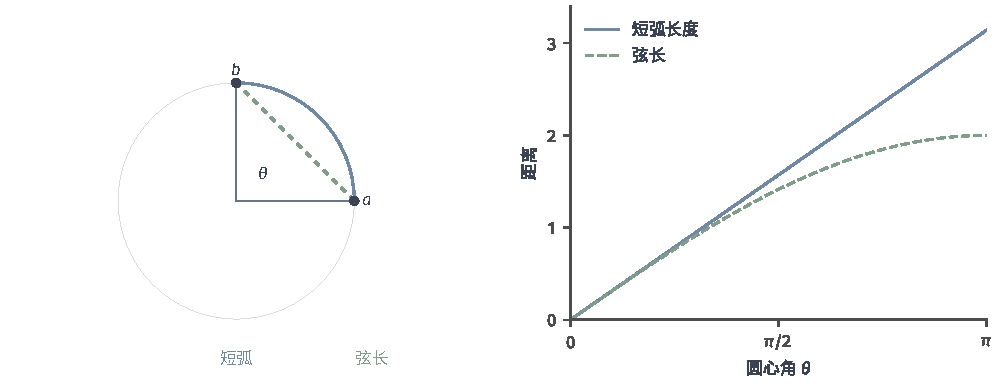
\includegraphics[width=169.0mm]{figures/01-mathematical-preliminaries-upper/02-linear-algebra-and-geometry/matplotlib/geometry-circle-distances/figure.pdf}
  \caption{完整单位圆的测地距离与环境弦长。左图夹角为$\pi/2$，
 蓝线为圆上的允许短弧，绿虚线为穿过圆内的环境线段；
 右图比较$\theta\in[0,\pi]$时的两种长度。完整圆允许选择两段弧中的较短者，
 不能与开中心线或二维开带的允许路径混用。图为解析教学示例。}
 \label{fig:geometry-circle-distances}
\end{figure*}

定义使用下确界是有意保留存在性问题。在穿孔平面
$\mathbb R^2\setminus\{\bm0\}$中，$(-1,0)^\top$与$(1,0)^\top$
之间可绕过任意小的圆孔，路径长度趋于$2$，却没有长度恰为$2$的允许路径。
哪些全局条件保证达到下确界，将在固定端点的最短路径问题中讨论。

\subsection{对象的等价关系}
\label{sec:geometry-equivalence-relations}
\label{sec:geometry-symmetry-group-actions}

坐标可改变，不意味着任务输出必须不变。整体旋转点带时，长度不变，
表示朝向的向量却应同步旋转；重排点记录的行，则只改变编号而不移动空间中的点。
要准确规定这些要求，先明确允许哪些变换、如何复合，再指定它们作用于什么对象。

\begin{definition}[群]
\label{def:geometry-group}
\term{群}（group）$G$是带有二元运算的集合。运算封闭且满足结合律，
存在恒等元$e$，每个$g\in G$都存在逆元$g^{-1}$。
\end{definition}
群描述可以接连施加、也可以撤销的变换规则。集合中若只有若干增强操作，
复合后不再属于该集合，或者裁剪已丢失信息而不可逆，就还不能直接称其为群。
群的抽象乘法与对象上的实际操作，通过群作用联系。

\begin{definition}[群作用]
\label{def:geometry-group-action}
\term{群作用}（group action）是映射$G\times\mathcal X\to\mathcal X$，
记$(g,x)\mapsto g\cdot x$，满足
\begin{equation}
 e\cdot x=x,\qquad (g_1g_2)\cdot x=g_1\cdot(g_2\cdot x)
 \label{eq:geometry-group-action}
\end{equation}
对所有$x\in\mathcal X$和$g_1,g_2\in G$成立。
\end{definition}
第二条把群乘法解释为先做$g_2$、再做$g_1$。
同一个群可以作用在不同空间上，具体作用必须给出；讨论光滑流形上的作用时，
还要另行要求相应映射光滑。


如果任务确实要忽略某类变换，就应把该变换关联的输入视为等价。
\term{轨道}（orbit）$G\cdot x=\{g\cdot x:g\in G\}$收集从$x$出发能够得到的
所有输入。定义$x\sim y$当且仅当存在$g\in G$使$y=g\cdot x$，这是等价关系：
恒等元保证反身，逆元保证对称，复合保证传递。轨道的集合称为轨道商$\mathcal X/G$。
这时才有明确依据说两个不同记录代表同一个等价输入。


轨道商在这里只是等价类集合。即使原空间光滑，也不能直接宣布商仍是同维或更低维
的光滑流形。例如平面上全部旋转组成的群$\mathrm{SO}(2)$作用于$\mathbb R^2$，
轨道按半径标记，
商可识别为$[0,\infty)$：原点的轨道只有一个点，其余轨道是圆。
商的端点不满足无边界一维流形的局部开区间条件。若讨论一般商的光滑结构，
需要补充作用的正则性条件，不能仅凭“去掉一个旋转自由度”作维数相减。

\section{运算与映射}
\label{sec:geometry-operations}

位置映射将一个点送到另一个点或一组特征，映射的叠加与复合组织多步作用。
点一旦变化，还需说明速度怎样传递、旧方向怎样搬到新位置，以及怎样从切向步产生可行的新点。
最后再从度量计算区域体积，为下一章的函数积分提供几何权重。

\subsection{空间之间的映射}
\label{sec:geometry-point-maps}

圆上位置可以映到横坐标，也可以映到另一个曲面上的位置。
要判断这样的映射是否光滑，先把两端位置都转成局部欧氏坐标。
设$F:\mathcal M\to\mathcal N$，用输入参数化$\varphi$与输出参数化$\psi$
记录后，$\psi^{-1}\circ F\circ\varphi$是欧氏开集之间的映射。
若所有适用图中的表达都光滑，就称$F$光滑；光滑过渡和链式法则保证换图不改变这个判断。
输出也可以是$\mathbb R^r$中的特征，而不一定是另一个弯曲空间中的位置。
例如单位圆上的$(x,y)\mapsto x$读取环境横坐标，仍是合法的光滑映射。

\subsection{映射的叠加}
\label{sec:geometry-map-addition}

映射叠加要求各分支具有共同定义域，输出落在同一个可加的线性空间。
若$F_j:\mathcal M\to V$、$a_j$固定，则
$F(p)=\sum_j a_jF_j(p)$定义新的映射；各分支光滑时，坐标表达逐项相加仍光滑。
这里不要求$\mathcal M=V$。若输出是球面位置，直接相加通常不再可行；
若另作归一化，还须排除和为零，并把归一化看作新的复合步骤。

点云分支可以各自接收整幅点云，再把同形特征相加；共享逐点分支也可以先产生
各点特征，再求和汇聚。两者的输入对象不同，不能仅凭代码中都有求和就视为同一个作用。

\subsection{映射的复合}
\label{sec:geometry-map-composition}
\label{sec:geometry-group-invariance-equivariance}


当$F:\mathcal M\to\mathcal N$、$H:\mathcal N\to\mathcal P$的中间对象匹配时，
$(H\circ F)(p)=H(F(p))$。下面用复合表达变换后的响应：
保持数值是不变性，按指定方式改变输出是等变性。
当对象是向量且作用保持线性组合时，可以直接用线性代数描述响应。
\begin{definition}[线性表示]
\label{def:geometry-linear-representation}
\term{线性表示}（linear representation）是映射
$\rho:G\to\operatorname{GL}(V)$，满足
\begin{equation}
 \rho(e)=\bm I,\qquad \rho(g_1g_2)=\rho(g_1)\rho(g_2),
 \label{eq:geometry-linear-representation}
\end{equation}
其中$\operatorname{GL}(V)$是向量空间$V$上全部可逆线性算子组成的群。
\end{definition}
它用线性算子实现群的复合规则。输入与输出可以取不同表示：
输入平面坐标按旋转矩阵变换，标量输出可以取$\rho(g)=1$，
方向向量输出则可取同一旋转矩阵。

平面旋转群$\mathrm{SO}(2)$由行列式为$1$的二维正交矩阵组成。
角度$\theta$对应
\begin{equation}
 \bm R(\theta)=
 \begin{bmatrix}\cos\theta&-\sin\theta\\\sin\theta&\cos\theta\end{bmatrix},
 \qquad
 \bm R(\theta_1)\bm R(\theta_2)=\bm R(\theta_1+\theta_2).
 \label{eq:geometry-planar-rotation-group}
\end{equation}
同一旋转可作用于一个点、整组点，或通过改变自变量作用于图像函数。
这些输入空间不同。对点带整体旋转时，坐标写成$\bm R(\theta)\Phi(s,u)$，
局部参数$(s,u)$可以不变；这是环境表示改变，并非必须重新定义内部位置。

有限集合$\{1,\ldots,n\}$的全部置换组成对称群$S_n$。
约定置换矩阵满足$(\bm P_\pi\bm X)_{i,:}=\bm X_{\pi^{-1}(i),:}$，
则$\bm P_{\pi_1\pi_2}=\bm P_{\pi_1}\bm P_{\pi_2}$。
对点云$\bm X\in\mathbb R^{n\times D}$，行置换改变记录顺序，
而$D$维旋转矩阵$\bm R$作用在坐标列上，写为$\bm X\bm R^\top$。矩阵乘法的外形相似，
实际被改变的对象和索引却不同。


\begin{definition}[不变映射]
\label{def:geometry-invariant-map}
群$G$作用于$\mathcal X$。映射$f:\mathcal X\to\mathcal Y$若满足
\begin{equation}
 f(g\cdot x)=f(x)\qquad(g\in G,\ x\in\mathcal X),
 \label{eq:geometry-invariant-map}
\end{equation}
称为对该作用\term{不变}（invariant）。
\end{definition}
不变映射在同一轨道上取相同值，因此可写成
$f=\widetilde f\circ\pi$，其中$\pi(x)=G\cdot x$是商映射。
令$\widetilde f(G\cdot x)=f(x)$之所以不依赖代表元，正是由不变性保证。
但$f$也可能把不同轨道映到同一输出；不变不等于保留了区分轨道的全部信息。


当输出必须保留位置或朝向时，合理要求是让它按约定同步变化。
\begin{definition}[等变映射]
\label{def:geometry-equivariant-map}
若$G$还作用于$\mathcal Y$，把输出作用记为$\rho(g)$，映射
$F:\mathcal X\to\mathcal Y$满足
\begin{equation}
 F(g\cdot x)=\rho(g)F(x)\qquad(g\in G,\ x\in\mathcal X),
 \label{eq:geometry-equivariant-map}
\end{equation}
则称为\term{等变}（equivariant）。输出作用不必线性；当$\mathcal Y$是向量空间
且$\rho$为线性表示时，右端才是相应线性算子的作用。
\end{definition}
例如预测点带朝向时，输入旋转后，输出向量也应旋转。
标量类别、位置坐标和分割掩码所需的响应不同，不变性不是比等变性更好的统一目标。
等变映射之后接不变汇总可得到不变输出；反过来，已丢弃朝向的信息通常不能恢复。

在点云上，对每行使用同一个映射$\phi$，令
$F(\bm X)_{i,:}=\phi(\bm X_{i,:})$，则第$i$行直接给出
\[
 F(\bm P_\pi\bm X)_{i,:}
 =\phi(\bm X_{\pi^{-1}(i),:})
 =(\bm P_\pi F(\bm X))_{i,:}.
\]
所以逐点共享映射对行置换等变。再对行求和，
$f(\bm X)=\sum_i\phi(\bm X_{i,:})$，重编号只改变求和次序，因而不变。
这证明了响应关系，尚未证明求和表示能够区分任务需要的全部点集。

平移作用的例子需要同时规定定义域。对全空间上的可积函数
$k,f\in L^1(\mathbb R^d)$，这里$L^1$表示绝对值积分有限的函数。
令$(T_{\bm a}f)(\bm x)=f(\bm x-\bm a)$，
卷积是将一个函数平移后与另一个相乘并积分：
\begin{align}
 (k*(T_{\bm a}f))(\bm x)
 &=\int_{\mathbb R^d}k(\bm x-\bm y)f(\bm y-\bm a)\,\mathrm d\bm y\\
 &=\int_{\mathbb R^d}k(\bm x-\bm a-\bm z)f(\bm z)\,\mathrm d\bm z
   =(T_{\bm a}(k*f))(\bm x).
 \label{eq:geometry-translation-convolution-equivariance}
\end{align}
变量替换$\bm z=\bm y-\bm a$说明卷积与平移可交换。
$L^1$条件使等式几乎处处成立，即除去一个Lebesgue零测集后成立。
若积分处处绝对收敛，例如一个函数连续有界、
另一个可积，就可以逐点理解。有限图像的零填充、裁剪和下采样可能破坏所声称的
平移等变性；循环平移配周期边界和只比较有效区域又是另外的作用，须逐项核对。

\begin{table*}[htbp]
 \centering\small
 \begin{tabularx}{\linewidth}{@{}lXX@{}}
 \toprule
 输入作用 & 不变输出 & 等变输出及其作用\\
 \midrule
 平面旋转$\bm x\mapsto\bm R\bm x$
 & $\lVert\bm x\rVert_2$ & $F(\bm x)=\bm x$，输出也乘$\bm R$\\
 点记录行置换$\bm X\mapsto\bm P\bm X$
 & 逐行映射后求和 & 逐行共享映射，输出行也乘$\bm P$\\
 全空间信号平移
 & 可积函数的全空间积分 & 与固定可积核卷积，输出信号同样平移\\
 \bottomrule
 \end{tabularx}
 \caption{先指定输入与输出作用，才能判断不变或等变。全空间信号的恒等式不自动适用于
 有裁剪、边界填充或下采样的有限窗口；结构响应也不保证表示保留了任务所需的全部信息。}
 \label{tab:geometry-invariance-equivariance}
\end{table*}
表~\ref{tab:geometry-invariance-equivariance}把同一个输入作用的两种输出要求并列，
区别在于输出应该忽略变换，还是记录变换后的对象。


群复合还可以构造相对位置表示。对实数位置$t$和频率$\omega$，
令$\bm R_\omega(t)=\bm R(\omega t)$。同时平移位置$s,t$不改变$t-s$，而旋转复合给出
\begin{equation}
 \bm R_\omega(s)^\top\bm R_\omega(t)=\bm R_\omega(t-s).
 \label{eq:geometry-rotary-relative-position}
\end{equation}
所以对固定二维向量$\bm q,\bm k$，
\begin{equation}
 (\bm R_\omega(s)\bm q)^\top(\bm R_\omega(t)\bm k)
 =\bm q^\top\bm R_\omega(t-s)\bm k.
 \label{eq:geometry-rotary-dot-product}
\end{equation}
多个频率块并置仍保留这一恒等式，位置引入的旋转因子只通过相对位移出现。
这不意味着整个注意力网络只依赖相对位置：$\bm q,\bm k$的生成、其他位置特征、
偏置、窗口与边界仍可能含绝对位置信息。单个非零频率块的周期为$2\pi/|\omega|$，
多频率组合的可区分范围需连同频率、数值精度和序列长度分析，不能据此承诺无限长度
无碰撞。这里比较的是指定代数变换；后文沿曲面搬运方向还要给出路径和联络，
不能把两种操作都简化为一次任意旋转。


若要进一步组织可复合的局部表示，可以简要使用\term{范畴}（category）：
它包含对象、对象之间的箭头及各对象的恒等箭头，
仅在端点匹配时复合箭头，复合满足结合律与恒等律。
函子（functor）把对象和箭头映到另一范畴，同时保持恒等与复合。
例如坐标区域间可复合的过渡可按这种方式记录。
这只是组合表示的延伸语言，本章的距离与同调推导均不依赖它，
也不因引入这些名称获得额外的恢复保证。

\subsection{切向量的映射}
\label{sec:geometry-tangent-maps}

例如圆上的点在移动时，其横坐标也随之变化；给定点的瞬时速度，就应能计算读数的瞬时变化。
因此，除了点映射本身，还要建立它对切向速度的作用。
对第\ref{sec:geometry-point-maps}节定义的光滑映射$F:\mathcal M\to\mathcal N$，
取输入、输出两端的局部参数化$\varphi,\psi$。
它在$\bm p$处的微分（differential）把输入速度转成输出速度：
\[
 \mathrm dF_{\bm p}(\bm v)
 =\left.\frac{\mathrm d}{\mathrm dt}F(\gamma(t))\right|_{t=0},
 \qquad\gamma(0)=\bm p,\quad\gamma'(0)=\bm v.
\]
若$\bm v=\bm J_\varphi(\bm z)\bm a$，令
$\bm w=\psi^{-1}(F(\bm p))$，则
\begin{equation}
 \mathrm dF_{\bm p}(\bm v)
 =\bm J_\psi(\bm w)
   \bm J_{\psi^{-1}\circ F\circ\varphi}(\bm z)\bm a.
 \label{eq:geometry-map-differential}
\end{equation}
右端只依赖初速度，不依赖实现速度的曲线，因此定义良好且线性。
坐标变换时两侧的Jacobian因链式法则相互抵消；
$\mathrm dF_{\bm p}:T_{\bm p}\mathcal M\to T_{F(\bm p)}\mathcal N$
是几何映射，矩阵只是其坐标记录。复合还满足
$\mathrm d(H\circ F)_{\bm p}=\mathrm dH_{F(\bm p)}\circ\mathrm dF_{\bm p}$。

对标量函数$f:\mathcal M\to\mathbb R$，微分读取速度引起的一阶数值变化。
\term{余切空间}（cotangent space）$T_{\bm p}^*\mathcal M$就是
$T_{\bm p}\mathcal M$的线性泛函空间，泛函的含义沿用
第\ref{sec:linear-algebra-scalar-readouts}节的有限维标量读取。
有限维向量空间上的全部线性读取组成其对偶空间（dual space）；
所以$\mathrm df_{\bm p}\in T_{\bm p}^*\mathcal M$，不是一个切向量。
沿用前面的局部坐标$(z^1,\ldots,z^d)$与坐标切基$\partial_i$，
其对偶基$\mathrm dz^i$满足$\mathrm dz^i(\partial_j)=\delta_{i,j}$，
也就是$\mathrm dz^i(\sum_j a^j\partial_j)=a^i$：它读出速度的第$i$个坐标系数。于是
\[
 \mathrm df=\sum_i\partial_i(f\circ\varphi)\,\mathrm dz^i,\qquad
 \mathrm df\!\left(\sum_i a^i\partial_i\right)
 =\sum_i\partial_i(f\circ\varphi)a^i.
\]
例如圆上$f(\cos\theta,\sin\theta)=\cos\theta$，
角速度$a$对应的数值变化为$-a\sin\theta$。
要把这个线性读取规则表示成“最陡方向”，还须指定方向长度，
第\ref{sec:geometry-point-optimization}节将用已经建立的度量，把这个读取规则表示为梯度。

\subsection{切向量的搬运}
\label{sec:geometry-tangent-transport}
\label{sec:geometry-connection-comparison}
\label{sec:geometry-riemannian-curvature}

\label{sec:geometry-cross-point-comparison-curvature}
\label{sec:geometry-parallel-transport}

沿路径计算长度时，每个位置只输出一个标量。若要问速度有没有转弯，
或相邻两点的方向是否一致，就必须比较不同切空间中的向量。
即使流形嵌在同一个欧氏空间内，直接相减也可能产生法向分量：
圆上恒速运动的速度导数指向圆心，却没有沿圆加速。
需要把环境变化与流形内的方向变化分开。下面建立联络、平行移动和曲率，
所用的Riemann几何基础可参见Lee的教材\scite{math-lee2018riemannian}。


把圆周上的单位切向速度画在每个位置，得到一个向量场。
沿圆周求它的环境导数会出现法向分量，但流形内的方向变化应仍是切向的。
下面用联络规定这种微分：它保持切向性，也保留求导对加法与函数乘积的规则。
联络据此比较邻近位置的方向，无须把所有切空间认作同一个固定子空间。

\begin{definition}[向量场与联络]
\label{def:geometry-connection}
光滑\term{向量场}（vector field）$\bm V$在每个$\bm p\in\mathcal M$选取
$\bm V(\bm p)\in T_{\bm p}\mathcal M$，其坐标分量光滑。
\term{联络}（connection）为两个光滑向量场$\bm U,\bm V$指定向量场
$\nabla_{\bm U}\bm V$，称为$\bm V$沿$\bm U$的
\term{协变导数}（covariant derivative），并满足
\[
 \begin{aligned}
 \nabla_{f\bm U+h\bm W}\bm V
   &=f\nabla_{\bm U}\bm V+h\nabla_{\bm W}\bm V,\\
 \nabla_{\bm U}(a\bm V+b\bm W)
   &=a\nabla_{\bm U}\bm V+b\nabla_{\bm U}\bm W,\\
 \nabla_{\bm U}(f\bm V)
   &=\bm U(f)\bm V+f\nabla_{\bm U}\bm V.
 \end{aligned}
\]
其中$f,h$为光滑函数，$a,b\in\mathbb R$，
$\bm U(f)=\mathrm df(\bm U)$为方向导数。
\end{definition}
第一项对求导方向按光滑函数线性，第二项对被求导对象按常数线性，
第三项则说明不能把第二项也加强为按光滑函数线性：
系数本身的变化必须保留。欧氏空间的普通方向导数满足这三项规则；
一般流形上，单独求坐标分量的导数不够，因为坐标切基本身也在变。

度量已经规定长度，新的导数应当与这一判断相容。
此外，非坐标方向场先后作用的顺序本来就可能不同，不能把这种差异误认为额外的几何扭转。
定义交换子$[\bm U,\bm V]$为对任意光滑$f$满足
\[
 [\bm U,\bm V](f)=\bm U(\bm V(f))-\bm V(\bm U(f))
\]
的向量场；在坐标基下，其第$k$个分量为
$\sum_i(U^i\partial_iV^k-V^i\partial_iU^k)$。
坐标方向$\partial_i,\partial_j$的交换子为零，一般方向场则未必。

\begin{example}[平面上不可交换的方向场]
\label{ex:geometry-plane-field-commutator}
在欧氏平面取$\bm U=\partial_x$、$\bm V=x\partial_y$。
$\bm U$始终沿$x$轴，$\bm V$沿$y$轴但其大小随$x$改变。
对任意光滑函数$f$，
\[
 \bm U(\bm V(f))=\partial_yf+x\partial_x\partial_yf,\qquad
 \bm V(\bm U(f))=x\partial_y\partial_xf,
\]
故$[\bm U,\bm V]=\partial_y$。先沿$x$方向移动，会改变随后沿$\bm V$移动的速度；
两个方向场的顺序差异在平面上就会出现。
欧氏空间的普通方向导数还给出
\[
 \nabla_{\bm U}\bm V=\partial_y,\qquad
 \nabla_{\bm V}\bm U=\bm0.
\]
二者之差恰是交换子。这个平坦例子说明，方向场本身随位置变化所产生的差异，
需要与几何结构额外产生的差异分开。
\end{example}

\begin{definition}[Levi--Civita联络]
\label{def:geometry-levi-civita-connection}
给定Riemann度量$g$，同时满足下列度量相容与无挠条件的联络，
称为它的\term{Levi--Civita联络}（Levi--Civita connection）：
\begin{align*}
 \bm U\bigl(g(\bm V,\bm W)\bigr)
 &=g(\nabla_{\bm U}\bm V,\bm W)+g(\bm V,\nabla_{\bm U}\bm W),\\
 \nabla_{\bm U}\bm V-\nabla_{\bm V}\bm U&=[\bm U,\bm V].
\end{align*}
\end{definition}
度量相容使内积的求导仍满足乘积法则；无挠规定联络在交换两个方向场时，
不产生交换子之外的差异。无挠\emph{不}声称
$\nabla_{\bm U}\nabla_{\bm V}\bm W
=\nabla_{\bm V}\nabla_{\bm U}\bm W$，后者涉及本节末尾的曲率。

每个光滑Riemann度量唯一确定这样的联络。其唯一性可以从两项条件直接看出：
轮换$\bm U,\bm V,\bm W$的度量相容等式，并用无挠条件消去交换项，得到
\begin{align}
 2g(\nabla_{\bm U}\bm V,\bm W)
 &=\bm U g(\bm V,\bm W)+\bm V g(\bm W,\bm U)
   -\bm W g(\bm U,\bm V)\notag\\
 &\quad+g([\bm U,\bm V],\bm W)-g([\bm V,\bm W],\bm U)
   +g([\bm W,\bm U],\bm V).
 \label{eq:geometry-koszul-formula}
\end{align}
右端只含已知度量、向量场和普通方向导数；正定性使其唯一确定
$\nabla_{\bm U}\bm V$。反过来，用此式定义该向量场，代入可检查联络的三条规则、
度量相容和无挠条件，因而也给出存在性。这个公式的用途是确定比较规则，
实际计算通常使用坐标系数或环境投影。

对继承欧氏度量的嵌入流形，设$\bm P_{\bm p}$为环境空间到
$T_{\bm p}\mathcal M$的正交投影，则
\begin{equation}
 \nabla_{\bm U}\bm V(\bm p)
 =\bm P_{\bm p}\,\mathrm d\bm V_{\bm p}(\bm U(\bm p)).
 \label{eq:geometry-projected-connection}
\end{equation}
这里把$\bm V$视为取值于环境$\mathbb R^D$的映射，先求环境导数再投影。
投影保持对切向量的内积，所以欧氏内积的乘积法则给出度量相容；
环境方向导数之差是已经切向的交换子，投影后仍不变，故也无挠。
由唯一性，这正是诱导度量的Levi--Civita联络。
若度量不是环境诱导度量，不能继续沿用这个欧氏正交投影公式。


现在固定路径$\gamma(t)$和起点切向量，希望沿路保持方向。
“保持”不是要求环境坐标分量不变，而是要求联络测得的变化为零。
在坐标基中写
$\nabla_{\partial_i}\partial_j=\sum_k\Gamma^k_{i,j}\partial_k$。
这些系数称为Christoffel符号，记录坐标切基随位置的变化；第\ref{sec:geometry-position-updates}节将从度量求出其表达式。
沿$\gamma(t)=\varphi(\bm z(t))$的向量
$\bm V(t)=\sum_jV^j(t)\partial_j$满足
\begin{equation}
 \frac{D\bm V}{\mathrm dt}
 =\sum_k\left(\dot V^k+
     \sum_{i,j}\Gamma^k_{i,j}(\bm z(t))\dot z^iV^j\right)\partial_k.
 \label{eq:geometry-covariant-derivative-along-path}
\end{equation}
第一项是分量变化，第二项修正坐标切基的变化；合起来才是坐标无关的协变导数。
对于欧氏诱导度量，式~\eqref{eq:geometry-projected-connection}沿路径写成
\[
 \frac{D\bm V}{\mathrm dt}
 =\bm P_{\gamma(t)}\frac{\mathrm d\bm V}{\mathrm dt},
\]
保留环境导数的切向部分。

\begin{definition}[平行移动]
\label{def:geometry-parallel-transport}
给定分段光滑路径$\gamma:[a,b]\to\mathcal M$和
$\bm v\in T_{\gamma(a)}\mathcal M$，沿路解
\[
 \frac{D\bm V}{\mathrm dt}=\bm0,\qquad \bm V(a)=\bm v.
\]
终值定义线性映射
$P_\gamma:T_{\gamma(a)}\mathcal M\to T_{\gamma(b)}\mathcal M$，
称为沿$\gamma$的\term{平行移动}（parallel transport）。
\end{definition}
坐标式是具有连续系数的线性常微分方程，初值唯一决定解；
沿有限段路径逐图求解并拼接即可，不要求流形完备。
反向路径给出逆映射，拼接路径对应映射复合。
对于Levi--Civita联络，
\[
 \frac{\mathrm d}{\mathrm dt}g(\bm V,\bm W)
 =g(D\bm V/\mathrm dt,\bm W)+g(\bm V,D\bm W/\mathrm dt)=0
\]
用于任意两个平行向量场。因此$P_\gamma$保持长度和夹角。
这个结论依赖度量相容，不能对任意联络直接宣称保距。

欧氏空间的直角坐标中$\Gamma^k_{i,j}=0$，平行移动保持向量的分量不变，
且与路径无关。球面则不同：向量必须始终切向，环境分量通常会改变，
不同路径的终值也可能不同。

\begin{example}[球面三段路径上的方向搬运]
\label{ex:geometry-sphere-parallel-transport}
在诱导度量的单位球面$\mathbb S^2$上，取
$N=(0,0,1)^\top$、$A=(1,0,0)^\top$、$B=(0,1,0)^\top$。
记三个坐标轴的单位向量为$\bm e_x,\bm e_y,\bm e_z$。
沿三条四分之一大圆弧$N\to A\to B\to N$搬运初始向量
$\bm V(N)=\bm e_x$。各段用$t\in[0,\pi/2]$参数化：
\[
 \begin{array}{c|c|c}
  \text{路径}&\gamma(t)&\bm V(t)\\ \hline
  N\to A&(\sin t,0,\cos t)^\top&(\cos t,0,-\sin t)^\top\\
  A\to B&(\cos t,\sin t,0)^\top&(0,0,-1)^\top\\
  B\to N&(0,\cos t,\sin t)^\top&(0,\sin t,-\cos t)^\top
 \end{array}
\]
每段都有$\gamma^\top\bm V=0$与$\lVert\bm V\rVert_2=1$。
第一段$\dot{\bm V}=-\gamma$，第二段$\dot{\bm V}=\bm0$，
第三段$\dot{\bm V}=\gamma$，环境导数全部是法向或零，投影后的协变导数为零。
两处接点的向量同为$-\bm e_z$，故三段连续拼接。
返回$N$时向量成为$\bm e_y$，与初始$\bm e_x$相差$\pi/2$。
若始终留在$N$，搬运则不改变向量，说明仅给起终点不能决定平行移动。
\end{example}

图~\ref{fig:geometry-sphere-parallel-transport}画出这些向量的沿路变化。
在$B\to N$段，向量与前进速度相反；保持方向不意味着向量必须指向前进方向。
\begin{figure}[htbp]
  \centering
  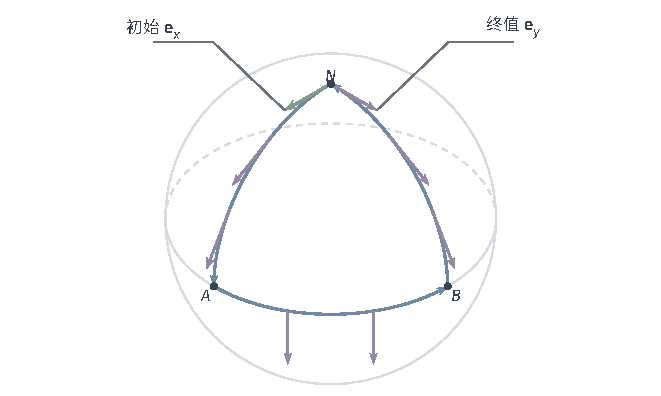
\includegraphics[width=112.0mm]{figures/01-mathematical-preliminaries-upper/02-linear-algebra-and-geometry/tikz/geometry-sphere-parallel-transport/figure.pdf}
  \caption{单位球面上沿$N\to A\to B\to N$的平行移动。
 蓝色为给定的三条大圆弧，紫箭头为例~\ref{ex:geometry-sphere-parallel-transport}
 中逐段计算的切向量。沿路协变导数为零，返回$N$后的方向却由初始箭头
 $\bm e_x$变为紫色终值箭头$\bm e_y$。
 箭头在三维中等长，投影到纸面后的长度可以不同。图为解析教学示例。}
 \label{fig:geometry-sphere-parallel-transport}
\end{figure}

这里的变换由路径和联络决定，不是任意选一个旋转来对齐环境向量。
前文群作用规定的是输入在指定变换下的响应；平行移动规定的是沿几何路径的方向比较，
即使二者有时都用矩阵表示，也不能据此互换。


球面闭路例子已经表明，搬运结果可以依赖路线。
为检测一个点附近的这种差异，可以比较沿两个方向先后求协变导数的结果。
方向场本身未必可交换，必须扣除$[\bm U,\bm V]$造成的变化，
剩下的才是联络对局部路径差异的响应。
这里有三个方向的不同职责：$\bm U,\bm V$指定小回路的两个方向，
另一个切向量$\bm W$是沿路搬运的箭头。给定前两个方向后，曲率作用在$\bm W$上，
检测绕路带来的方向变化；$\bm W$不必等于路径的前进速度。

\begin{definition}[Riemann曲率]
\label{def:geometry-riemann-curvature}
本章取曲率符号约定
\begin{equation}
 R(\bm U,\bm V)\bm W
 =\nabla_{\bm U}\nabla_{\bm V}\bm W
  -\nabla_{\bm V}\nabla_{\bm U}\bm W
  -\nabla_{[\bm U,\bm V]}\bm W.
 \label{eq:geometry-riemann-curvature}
\end{equation}
Levi--Civita联络的这个算子称为\term{Riemann曲率}（Riemann curvature）。
在点$\bm p$处，其值只依赖$\bm U,\bm V,\bm W$在该点的值，
而不依赖它们在附近的具体延拓。
\end{definition}
最后一项消掉方向场选择带来的导数项，使$R$成为按点定义的张量，即对点处方向多线性且不依赖坐标的对象。
例如在$\bm V$前乘光滑函数时，前两项会出现关于该函数的导数，
第三项恰好抵消它们。比较小闭路平行移动与恒等映射时，以闭路面积为尺度的
首项由$R(\bm u,\bm v)$控制；这个首项也可能为零，具体正负随绕行方向约定改变。
有限大闭路的总效应不能简单用某一点的曲率乘面积代替。

曲率算子仍含多个方向。选定一个二维切平面，可以用它给出一个标量曲率，
比较该平面内的局部几何。
\begin{definition}[截面曲率]
\label{def:geometry-sectional-curvature}
若$\bm u,\bm v\in T_{\bm p}\mathcal M$线性无关，
定义它们张成平面的\term{截面曲率}（sectional curvature）为
\begin{equation}
 K_{\bm p}(\bm u,\bm v)
 =\frac{g(R(\bm u,\bm v)\bm v,\bm u)}
 {g(\bm u,\bm u)g(\bm v,\bm v)-g(\bm u,\bm v)^2}.
 \label{eq:geometry-sectional-curvature}
\end{equation}
分母是该平行四边形的平方面积，正定性保证它为正。
\end{definition}
更换同一平面的基不改变比值。二维流形每点只有整个切平面这个选择，
所得量就是Gauss曲率；一维流形没有二维切平面，不能给圆硬套一个截面曲率数值。
一维Riemann曲率张量恒为零。

平面采用欧氏度量时，直角坐标中的联络系数为零，故$R=0$。
半径$R_0$的圆柱取局部参数
$(s,z)\mapsto(R_0\cos(s/R_0),R_0\sin(s/R_0),z)$，
诱导度量为$\mathrm ds^2+\mathrm dz^2$，
所以局部联络系数和内在曲率同样为零。
圆柱在环境中明显弯曲，却可以局部无伸缩地展开成平面；
把圆柱卷起来改变的是嵌入形状，不是这个局部度量。

半径$R_0$的球面则不同。对切向场，微分
$\langle\bm V,\bm p\rangle=0$给出
$\langle\mathrm d\bm V(\bm U),\bm p\rangle=-\langle\bm V,\bm U\rangle$，
因此
\[
 \nabla_{\bm U}\bm V
 =\mathrm d\bm V(\bm U)+\frac{g(\bm U,\bm V)}{R_0^2}\bm p.
\]
将其代入曲率定义，环境二阶导数与交换子相消；
再投影时，法向系数的导数被消去，而$\mathrm d\bm p(\bm U)=\bm U$留下
\[
 R(\bm U,\bm V)\bm W
 =\frac1{R_0^2}\bigl(g(\bm V,\bm W)\bm U-g(\bm U,\bm W)\bm V\bigr).
\]
代入式~\eqref{eq:geometry-sectional-curvature}便得任意截面
$K=1/R_0^2>0$。这也核对了本章曲率符号：球面的曲率为正。

在图~\ref{fig:geometry-sphere-parallel-transport}所用的单位球面北极
$N=(0,0,1)^\top$，取正交单位切向量$\bm u=\bm e_x$、$\bm v=\bm e_y$。
若被搬运的箭头取$\bm W=\bm v$，上式具体给出
\[
 R(\bm u,\bm v)\bm v=\bm u,\qquad
 K_N(\bm u,\bm v)=
 \frac{g(\bm u,\bm u)}{1\cdot1-0^2}=1.
\]
分子读出曲率作用后沿$\bm u$的分量，分母消去所选两方向围成的面积平方的尺度。
这里计算的是北极附近一个截面的局部曲率；前面的三段球面图则展示有限闭路的最终搬运。
缩小回路后观察方向变化的首项，才把这种沿路变化与局部曲率联系起来。

第\ref{sec:geometry-sampled-local-linearization}节将估计切平面；其法向误差需要与内在曲率区分。圆的一维方向沿环境空间转动，
产生二阶法向偏离，但其内在Riemann曲率为零；
圆柱也有法向弯曲而内在平坦。二维开带本来就是平面的开集，
式~\eqref{eq:geometry-strip-metric}虽有随位置变化的系数，内在曲率仍为零。
这些例子说明，法向二阶误差和Christoffel系数都不能单独作为内在非零曲率的证据。
局部曲率也不替代拓扑：平面与圆柱局部同样平坦，整体的环却不同；
局部零曲率本身不保证任意全局闭路上的搬运都平凡。

\subsection{对象的位置更新}
\label{sec:geometry-position-updates}
\label{sec:geometry-geodesic-motion-minimization}

\label{sec:geometry-geodesic-motion}

给定当前位置和一个切向步，直接沿环境直线前进通常会离开流形。
让速度沿自身路径平行移动，就能在保持初始速度大小的同时产生流形内的新位置。

\begin{definition}[测地线]
\label{def:geometry-geodesic}
相对于Riemann流形的Levi--Civita联络，采用仿射参数的曲线$\gamma$若满足
\[
 \frac{D\dot\gamma}{\mathrm dt}=\bm0,
\]
称为\term{测地线}（geodesic）。
\end{definition}
它没有切向加速度，速度沿自身路径作平行移动。
度量相容进一步给出
$\frac{\mathrm d}{\mathrm dt}\lVert\dot\gamma\rVert_g^2
=2g(D\dot\gamma/\mathrm dt,\dot\gamma)=0$，因此速度大小恒定。
环境加速度仍可非零，例如球面大圆需要法向加速度才能留在球面。

“仿射参数”说明换元$t=ar+b$、$a\neq0$保留这个方程。
一般换元则产生
\[
 \frac{D}{\mathrm dr}\frac{\mathrm d\gamma}{\mathrm dr}
 =(\tau'(r))^2\frac{D\dot\gamma}{\mathrm dt}
   +\tau''(r)\dot\gamma.
\]
非匀速参数化可以描出相同几何轨迹，却不再满足零协变加速度。
因此不能把路径长度的任意重参数化不变性照搬到这个运动方程。

要在坐标中求解，先用式~\eqref{eq:geometry-koszul-formula}取
$\bm U=\partial_i,\bm V=\partial_j,\bm W=\partial_\ell$。
坐标方向交换子为零，于是
\[
 2\sum_k g_{k,\ell}\Gamma^k_{i,j}
 =\partial_i g_{j,\ell}+\partial_j g_{i,\ell}-\partial_\ell g_{i,j}.
\]
乘逆度量便得到Christoffel符号
\begin{equation}
 \Gamma^k_{i,j}
 =\frac12\sum_{\ell=1}^d g^{k,\ell}
  \left(\frac{\partial g_{\ell,j}}{\partial z^i}
       +\frac{\partial g_{i,\ell}}{\partial z^j}
       -\frac{\partial g_{i,j}}{\partial z^\ell}\right),
 \qquad [g^{i,j}]=\bm G^{-1}.
 \label{eq:geometry-christoffel-symbols}
\end{equation}
将$\bm V=\dot\gamma=\sum_j\dot z^j\partial_j$代入
式~\eqref{eq:geometry-covariant-derivative-along-path}，测地条件成为
\begin{equation}
 \ddot z^k+\sum_{i,j=1}^d
 \Gamma^k_{i,j}(\bm z)\dot z^i\dot z^j=0.
 \label{eq:geometry-geodesic-equation}
\end{equation}
要判断这组系数是否表示点处的几何对象，需要区分几何张量与一张普通分量表。
这里的几何张量（geometric tensor）是点处、与坐标无关的多线性对象；
换基只对它的各个输入和输出作线性变换。因此，零分量表换基后仍为零。
Christoffel符号不满足这一规律。以正半轴的欧氏度量为例，
在坐标$x>0$中有$g_{x,x}=1$、$\Gamma^x_{x,x}=0$；
改用$x=e^u$后，$g_{u,u}=e^{2u}$，式~\eqref{eq:geometry-christoffel-symbols}给出
\[
 \Gamma^u_{u,u}=\frac12 e^{-2u}\frac{\mathrm d}{\mathrm du}e^{2u}=1.
\]
所以Christoffel符号是联络的坐标系数，不是张量。
基向量的变化与这些系数共同组成协变加速度，后者及所得曲线仍是几何对象。

光滑系数使这个二阶方程在给定
$\gamma(0)=\bm p$、$\dot\gamma(0)=\bm v$后具有局部唯一解，
并光滑依赖初值。这里“局部”同时限制时间和坐标覆盖范围；
可以换图延拓，但若路径有限时间离开流形，延拓就会失败。
开单位球内的欧氏直线从原点出发，以速度$2\bm e_1$前进，
在$t=1/2$时便到达不属于该流形的边界，不能默认解存在至$t=1$。

\begin{definition}[指数映射]
\label{def:geometry-exponential-map}
对给定$\bm p$，若初速度$\bm v$的测地线$\gamma_{\bm v}$存在至$t=1$，
定义
\[
 \operatorname{Exp}_{\bm p}(\bm v)=\gamma_{\bm v}(1).
\]
它称为$\bm p$处的\term{指数映射}（exponential map），
其定义域至少包含$T_{\bm p}\mathcal M$中零向量的一个邻域。
\end{definition}
初速度缩放对应时间缩放：
$\operatorname{Exp}_{\bm p}(t\bm v)=\gamma_{\bm v}(t)$，只在两边均有定义时使用。
因而$\operatorname{Exp}_{\bm p}(\bm0)=\bm p$且
$\mathrm d(\operatorname{Exp}_{\bm p})_{\bm0}=\operatorname{id}_{T_{\bm p}\mathcal M}$。
逆函数定理保证在足够小邻域中它是微分同胚；
这为用切向量表示附近点提供了一种局部方式，不保证全局一一对应。

单位球面上，$\bm v\perp\bm p$、$r=\lVert\bm v\rVert_2$时，
\begin{equation}
 \operatorname{Exp}_{\bm p}(\bm v)
 =\cos r\,\bm p+\frac{\sin r}{r}\bm v,
 \label{eq:geometry-sphere-exponential}
\end{equation}
$r=0$时按连续延拓取$\bm p$。
对应曲线$\gamma(t)=\cos(tr)\bm p+\sin(tr)\bm v/r$
满足$\lVert\gamma(t)\rVert_2=1$、初速度为$\bm v$，
且$\ddot\gamma=-r^2\gamma$为纯法向，所以确实解测地线方程。
所有方向上长度为$\pi$的初速度都到达对跖点$-\bm p$；
即使映射处处有定义，也未必全局单射。


切向量$\bm v$给出可行的瞬时方向，有限位移$\bm p+\bm v$却通常离开流形。
指数映射给出一种更新，但求解精确测地线可能昂贵。
如果只需保证一阶变化正确，可以使用更易计算的局部返回映射。

\begin{definition}[回缩]
\label{def:geometry-retraction}
对每个$\bm p$，在$T_{\bm p}\mathcal M$的零向量邻域中给定
$\mathcal R_{\bm p}(\bm v)\in\mathcal M$，并使其光滑依赖$(\bm p,\bm v)$。
若
\[
 \mathcal R_{\bm p}(\bm0)=\bm p,\qquad
 \mathrm d(\mathcal R_{\bm p})_{\bm0}[\bm v]=\bm v,
\]
则称这一族映射为\term{回缩}（retraction）。
\end{definition}
第一项保留起点，第二项保留初速度。它不要求沿$t\mapsto\mathcal R_{\bm p}(t\bm v)$
作精确测地运动，也不要求任意大步长都在定义域中。
指数映射是一种局部回缩，其他回缩可有不同的高阶误差。


这些映射接收当前位置与一个小切向步，输出新位置。
它们只规定一步怎样保持可行；怎样选择方向、步长以及整个序列是否收敛，是后面的求解与收敛问题。

\subsection{区域的体积计算}
\label{sec:geometry-riemannian-volume}

要比较区域的大小，路径的一维长度还不够，需要给小区域规定体积。
坐标切基围成的微小平行体，其平方体积是Gram行列式$\det\bm G$，
因此几何体积元为
\begin{equation}
 \mathrm dV_g=\sqrt{\det\bm G(\bm z)}\,\mathrm d\bm z.
 \label{eq:geometry-riemannian-volume}
\end{equation}
这是由度量产生的测度密度，不要求先为流形选定全局朝向。
一维时给出长度，二维时给出面积。

坐标变换$\bm z=\psi(\bm v)$下，
$\det\widetilde{\bm G}=(\det\bm A)^2\det\bm G$，所以
\[
 \sqrt{\det\widetilde{\bm G}}\,\mathrm d\bm v
 =\sqrt{\det\bm G(\psi(\bm v))}\,|\det\bm A|\,\mathrm d\bm v.
\]
它正是多元积分换元中的Jacobian因子，故对可积函数所得积分不依赖坐标。
跨图时必须避免把重叠区域重复计数，可分割成可测片段分别积分；
光滑计算也可使用从属于图册、和为$1$的局部权重来拼接。

点带中$\sqrt{\det\bm G}=1+u/R>0$，
小盒$\mathrm ds\,\mathrm du$在外侧对应较大面积。
中心线限制为$u=0$后的一维体积元是$\mathrm ds$，不是把二维面积直接代入。
若样本相对几何体积有密度$q$，其分布测度是$q\,\mathrm dV_g$；
当样本独立同分布地取自这个测度，且$\int|f|q\,\mathrm dV_g<\infty$时，
简单样本平均的期望是$\int fq\,\mathrm dV_g$；大数定律还保证它收敛到这个
加权积分。它并非自动近似$\int f\,\mathrm dV_g$。
几何体积与采样权重的差别将在离散平滑目标中再次出现。

当前开带无流形边界，但不是紧集。需要边界积分时，将另取有分片光滑边界的
截断闭域，并声明函数在边界的行为；不能只因图上画有虚线就把它当作同一个积分问题。

\section{方程与优化}
\label{sec:geometry-equations-optimization}

前面的运算可以计算已知点或方向的响应，现在用它们求未知对象。
给定两两距离时，未知量是一组坐标；给定位置与速度时，未知量是一条运动轨迹。
若改为给定两个端点，还需比较允许路线的长度。最后在流形中寻找目标值最小的点，
其可行更新将调用微分、度量和回缩。

\subsection{距离信息下的坐标重构}
\label{sec:geometry-distance-coordinate-embedding}

设只知道$n$个点之间的距离，能否给它们安排欧氏坐标，并精确保留这些距离？
先从反方向计算。将$\bm y_1,\ldots,\bm y_n\in\mathbb R^d$按行组成
$\bm Y\in\mathbb R^{n\times d}$。定义~\ref{def:linear-algebra-gram-matrix}中的
\term{Gram矩阵}$\bm B=\bm Y\bm Y^\top$记录两两内积，平方距离则为
\begin{equation}
  \delta_{i,j}=\lVert\bm y_i-\bm y_j\rVert_2^2
  =b_{i,i}+b_{j,j}-2b_{i,j}.
  \label{eq:geometry-distance-from-gram}
\end{equation}
距离不记录原点：将全部点平移同一个向量，差向量不变，内积却会改变。
因此从距离恢复内积前，需要先固定平移自由度。

把点云均值选为原点。令$\bm1\in\mathbb R^n$为全一向量，定义
\begin{equation}
  \bm J=\bm I_n-\frac1n\bm1\bm1^\top.
  \label{eq:geometry-centering-matrix}
\end{equation}
它满足$\bm J^\top=\bm J$、$\bm J^2=\bm J$和$\bm J\bm1=\bm0$；
$\bm J\bm Y$从每行减去样本均值。若$\bm\Delta=[\delta_{i,j}]$，
式~\eqref{eq:geometry-distance-from-gram}写成
\[
  \bm\Delta=\operatorname{diag}(\bm B)\bm1^\top
  +\bm1\operatorname{diag}(\bm B)^\top-2\bm B.
\]
左右各乘$\bm J$，前两项消失。对于已中心化的坐标，
$\bm J\bm Y=\bm Y$，于是
\begin{equation}
  \bm B=-\frac12\bm J\bm\Delta\bm J.
  \label{eq:geometry-double-centering}
\end{equation}
这称为\term{双重中心化}（double centering）：在两个点索引上消去均值项，
把平方距离转成以点云中心为原点的内积。此时尚未作低维投影。

任何真实坐标产生的Gram矩阵都半正定，因为
$\bm c^\top\bm B\bm c=\lVert\bm Y^\top\bm c\rVert_2^2\geq0$。
要证明这个条件也足够，需要排除双重中心化过程中丢失了某种非零距离差。

\begin{lemma}[双重中心化核的形式]
\label{lem:geometry-double-centering-kernel}
若对称矩阵$\bm H\in\mathbb R^{n\times n}$满足$\bm J\bm H\bm J=\bm0$，
则存在$\bm a\in\mathbb R^n$使
$\bm H=\bm1\bm a^\top+\bm a\bm1^\top$。
若另有$h_{i,i}=0$对全部$i$成立，则$\bm H=\bm0$。
\end{lemma}
\begin{proof}
令$\bm m=\bm H\bm1/n$、$\mu=\bm1^\top\bm H\bm1/n^2$。展开假设得到
\[
  \bm H=\bm1\bm m^\top+\bm m\bm1^\top-\mu\bm1\bm1^\top.
\]
取$\bm a=\bm m-(\mu/2)\bm1$即得所需形式。其对角元为$h_{i,i}=2a_i$，
故零对角条件迫使每个$a_i=0$，进而$\bm H=\bm0$。
\end{proof}

\begin{theorem}[有限距离的欧氏坐标重构]
\label{thm:geometry-euclidean-distance-embedding}
设$\bm\Delta\in\mathbb R^{n\times n}$对称且对角元为零，并令
$\bm B=-\bm J\bm\Delta\bm J/2$。矩阵$\bm\Delta$是某组欧氏点的平方距离矩阵，
当且仅当$\bm B$半正定。精确保留全部距离所需的最小欧氏维数为
$r=\operatorname{rank}(\bm B)$。
\end{theorem}
\begin{proof}
若已有欧氏点，先中心化，式~\eqref{eq:geometry-double-centering}便给出
$\bm B=\bm Y\bm Y^\top$，所以$\bm B$半正定。

反过来，半正定性和谱定理给出紧谱分解
$\bm B=\bm Q_r\bm\Lambda_r\bm Q_r^\top$，其中$\bm\Lambda_r$含$r$个正特征值。
取
\begin{equation}
  \bm Y=\bm Q_r\bm\Lambda_r^{1/2},
  \label{eq:geometry-classical-scaling-coordinates}
\end{equation}
则$\bm Y\bm Y^\top=\bm B$。又因$\bm B\bm1=\bm0$，
$\lVert\bm Y^\top\bm1\rVert_2^2=\bm1^\top\bm B\bm1=0$，坐标已中心化。
用式~\eqref{eq:geometry-distance-from-gram}从$\bm B$生成$\bm\Delta'$。
$\bm\Delta'$与$\bm\Delta$的双重中心化均为$\bm B$，两者之差对称、
对角为零且双重中心化为零。前一引理遂给出$\bm\Delta'=\bm\Delta$。

任意$\mathbb R^k$中的坐标矩阵所产生的Gram矩阵秩至多为$k$，
因此精确重构要求$k\geq r$；上述构造又在$k=r$时达到要求。
$r=0$时全部点重合，可视为嵌入零维空间。
\end{proof}

这个判据是经典尺度分析的代数核心。$\bm B$有负特征值时，输入关系不能被精确实现为
欧氏平方距离。逐对测量的距离误差可能造成负谱；直接由一组带噪坐标精确计算的距离
却仍来自欧氏点，其Gram矩阵不会仅因坐标带噪而失去半正定性。后者重构的是观测点，
不是噪声发生前的潜在点。

距离保留了相对位置，却不能确定绝对位置、朝向或手性。对正交矩阵
$\bm Q\in\mathbb R^{r\times r}$和平移$\bm a$，令
$\widetilde{\bm y}_i=\bm Q\bm y_i+\bm a$，则
\[
 \lVert\widetilde{\bm y}_i-\widetilde{\bm y}_j\rVert_2
 =\lVert\bm Q(\bm y_i-\bm y_j)\rVert_2
 =\lVert\bm y_i-\bm y_j\rVert_2.
\]
正交变换既含旋转，也含反射。中心化只消去平移，不能选择唯一朝向。

对于中心化的最小维坐标，这也是全部不确定性。设
$\bm Y,\widetilde{\bm Y}\in\mathbb R^{n\times r}$均列满秩并产生相同距离，
则双重中心化给出相同$\bm B$。它们的列空间都等于$\bm B$的值域。
对$\bm B=\bm Q_r\bm\Lambda_r\bm Q_r^\top$定义
$\bm M=\bm\Lambda_r^{-1/2}\bm Q_r^\top\bm Y$，可得
\[
 \bm Y=\bm Q_r\bm\Lambda_r^{1/2}\bm M,\qquad
 \bm M\bm M^\top
 =\bm\Lambda_r^{-1/2}\bm Q_r^\top\bm B\bm Q_r
   \bm\Lambda_r^{-1/2}=\bm I_r.
\]
方阵$\bm M$因而正交。写$\bm M=\bm U^\top$，对另一组坐标同样得到
$\widetilde{\bm Y}=\bm Q_r\bm\Lambda_r^{1/2}\widetilde{\bm U}^\top$，
于是$\widetilde{\bm Y}=\bm Y\bm U\widetilde{\bm U}^\top$。
重复特征值允许坐标轴在对应子空间内旋转；更高维实现的额外方向不含点云信息，
两组点仍在各自张成空间之间具有保距正交对应。

\begin{example}[三个点能否放在一条直线上]
\label{ex:geometry-three-point-embedding}
取$\bm y_1=(-1,0)^\top$、$\bm y_2=(0,1)^\top$、
$\bm y_3=(1,0)^\top$，其均值是$(0,1/3)^\top$。平方距离与中心化结果为
\[
 \bm\Delta=\begin{bmatrix}0&2&4\\2&0&2\\4&2&0\end{bmatrix},
\]
\begin{equation}
 -\frac12\bm J\bm\Delta\bm J
 =\begin{bmatrix}
  10/9&-2/9&-8/9\\
  -2/9&4/9&-2/9\\
  -8/9&-2/9&10/9
 \end{bmatrix}.
 \label{eq:geometry-three-point-centered-gram}
\end{equation}
正特征值为$2$和$2/3$，所以精确重构需要二维。
若只保留特征值$2$对应的水平方向，端点间距离仍为$2$，
顶点到两端的距离却从$\sqrt2$变成$1$；这是一种近似，不是另一份精确坐标。
\end{example}

这里必须区分谱近似的目标。若$\bm B$半正定，保留最大$k<r$个特征值时，
定理~\ref{thm:matrix-analysis-best-low-rank}保证Gram矩阵的Frobenius误差最小，
平方误差为$\sum_{j>k}\lambda_j^2$。在一组给定中心化坐标上作对应PCA投影，
坐标平方重构误差则为$\sum_{j>k}\lambda_j$。若原距离为
$d_{i,j}=\sqrt{\delta_{i,j}}$，近似坐标为$\widetilde{\bm y}_i$，
还可以直接比较逐对距离，例如把距离应力（distance stress）取为
\[
 \sum_{i<j}
 \bigl(\lVert\widetilde{\bm y}_i-\widetilde{\bm y}_j\rVert_2-d_{i,j}\bigr)^2.
\]
它比较距离，前两种误差分别比较内积和坐标，因此优化目标不同。
最大相对距离误差则比较
\[
 \max_{\substack{i<j\\d_{i,j}>0}}
 \frac{\bigl|\lVert\widetilde{\bm y}_i-\widetilde{\bm y}_j\rVert_2-d_{i,j}\bigr|}
 {d_{i,j}}.
\]
全体点重合时不使用这个比值准则。对含负谱的$\bm B$，保留最大的至多$k$个正特征值给出
半正定秩至多$k$约束下的Frobenius近似；舍弃负谱的大小仍须与测量误差比较。

有限坐标重构也不证明潜在集合是一张光滑曲面。即使点落在圆上，输入欧氏距离记录的仍是
弦长，不能把保弦长的坐标自动解释为沿圆排列的一维坐标。要表达连续对象的自由度，
必须另行给出局部模型。

\subsection{初值条件下的测地轨迹求解}
\label{sec:geometry-geodesic-initial-value}

给定$\gamma(0)=\bm p$与$\dot\gamma(0)=\bm v$，求满足
式~\eqref{eq:geometry-geodesic-equation}的轨迹。把二阶方程改写为$(z,\dot z)$的一阶系统，
局部光滑系数保证解在初值附近存在唯一。这里固定的是位置与速度，不是两个端点。
在重叠坐标图中，已有解与换图后的解由唯一性拼接，从而得到最大延拓区间。
只要位置与速度留在一组系数受控的紧区域内，就可继续局部求解；
流形缺口或无界离开会阻止这个过程。

完整单位球面上，取$\bm p\in S^{D-1}$、$\bm v\perp\bm p$，则
$\gamma(t)=\cos(t\lVert\bm v\rVert_2)\bm p
+\sin(t\lVert\bm v\rVert_2)\bm v/\lVert\bm v\rVert_2$
对全部$t$存在，$\bm v=\bm0$时取恒定轨迹。开球的直线却可能有限时间到达缺失边界。
第\ref{sec:geometry-endpoint-minimizing-path}节的完备性条件将给出全局延拓保证，
但初值的唯一性并不保证指定端点之间只有一条路径。

\subsection{端点约束下的最短路径求解}
\label{sec:geometry-endpoint-minimizing-path}

现在给定$\bm p,\bm q$，要求找到达到
式~\eqref{eq:geometry-geodesic-distance}下确界的路径。
其与测地方程的联系可通过路径能量建立。固定时间区间$[a,b]$，定义
\[
 E(\gamma)=\frac12\int_a^b\lVert\dot\gamma\rVert_g^2\,\mathrm dt.
\]
由Cauchy--Schwarz不等式，
$L_g(\gamma)^2\leq2(b-a)E(\gamma)$，等号恰对应几乎处处恒定的速度大小。
因此对可作匀速参数化的非退化路径，最小化长度可联系到固定时间的能量最小化；
能量本身却不具有长度那样的任意重参数化不变性。

在局部坐标中，Lagrange函数为
$\mathscr L(\bm z,\dot{\bm z})=\frac12\sum_{i,j}g_{i,j}(\bm z)\dot z^i\dot z^j$。
取光滑扰动$\bm h$，满足$\bm h(a)=\bm h(b)=\bm0$，并令
$\bm z_\varepsilon(t)=\bm z(t)+\varepsilon\bm h(t)$。
取足够小的$\varepsilon$使路径仍在坐标域内。
若$\varphi$为当前坐标的参数化，一阶变分就是把整条路径沿这个方向改变后，
能量关于扰动幅度的导数：
\[
 \delta E[\bm h]
 =\left.\frac{\mathrm d}{\mathrm d\varepsilon}
 E(\varphi\circ\bm z_\varepsilon)\right|_{\varepsilon=0}.
\]
对积分求导并分部积分，得到
\[
 \delta E[\bm h]
 =\int_a^b\sum_k\left(
 \frac{\partial\mathscr L}{\partial z^k}
 -\frac{\mathrm d}{\mathrm dt}
     \frac{\partial\mathscr L}{\partial\dot z^k}\right)h^k\,\mathrm dt.
\]
边界项因固定端点消失。驻定要求任意这样的$\bm h$都使变分为零，
因此括号中每个系数都必须为零：若某个连续系数在一点非零，
就在它保持同号的小邻域内取一个同号、光滑且在邻域外为零的扰动，
相应积分便不为零，产生矛盾。计算括号中的两个偏导得
\[
 \begin{aligned}
 \frac{\partial\mathscr L}{\partial z^k}
   &=\frac12\sum_{i,j}\partial_k g_{i,j}\dot z^i\dot z^j,\\
 \frac{\mathrm d}{\mathrm dt}
    \frac{\partial\mathscr L}{\partial\dot z^k}
   &=\sum_j g_{k,j}\ddot z^j+
     \sum_{i,j}\partial_i g_{k,j}\dot z^i\dot z^j.
 \end{aligned}
\]
对第二行的速度乘积对称化后，Euler--Lagrange方程为
\[
 \sum_jg_{k,j}\ddot z^j+
 \frac12\sum_{i,j}
  (\partial_i g_{k,j}+\partial_j g_{k,i}-\partial_k g_{i,j})
  \dot z^i\dot z^j=0.
\]
乘$\bm G^{-1}$即得式~\eqref{eq:geometry-geodesic-equation}。
跨图路径可对各段内支撑的扰动分别推导，得到相同几何方程。
这说明光滑匀速最短路必为测地线，不说明每个能量驻点都是最短路。

指数映射给出描述这些局部路径的区域。取零切向量附近的小开集$V$，
要求$\bm v\in V$时$t\bm v\in V$对$0\leq t\leq1$成立，
且$\operatorname{Exp}_{\bm p}$在$V$上为微分同胚。
它的像称为$\bm p$的正规邻域（normal neighborhood），
其中每个点都用一个初速度表示，径向路径对应$t\bm v$。
标准局部最短性结论保证可以把这个区域取到足够小，
使径向测地线段在邻域内达到端点间的最短长度。
还可进一步选择凸正规邻域（convex normal neighborhood），
让其中任意两点由唯一的邻域内最短测地线连接，整条线段留在该邻域中。
这里“凸”指测地线连接的性质，不是要求环境中的欧氏直线段留在区域内。
这项结论利用指数映射和径向、横向变化的正交性，不是只凭微分方程存在唯一性得到的。
离开这种局部范围后，其他路线可能更短。
若一段测地线达到$d_g$，称为\term{长度最短测地线}（length-minimizing geodesic）。

完整单位圆上，从$(1,0)^\top$到$(0,-1)^\top$的逆时针弧长为$3\pi/2$，
顺时针弧长为$\pi/2$。两条匀速圆弧都满足零协变加速度，
只有后者达到距离。相同的初值局部运动规则不承担全局路线比较。
割点研究从某点出发的测地线何时失去最短性，
共轭点涉及相邻测地线的聚焦与变分退化；这些进一步判据不在本章展开，
不能据术语本身判定一条路径最短。

\begin{theorem}[Hopf--Rinow定理的最短路存在性结论]
\label{thm:geometry-hopf-rinow-existence}
设$(\mathcal M,g)$为有限维、连通、无边界的光滑Riemann流形。
若它关于$d_g$完备，则任意两点之间存在长度最短测地线。
此时任意初速度的测地运动也可以延拓到所有实数时间。
\end{theorem}
这里引用这一定理的存在性结论，不展开完整等价条件及证明。
完备性是每个$d_g$-Cauchy序列都在$\mathcal M$内收敛；
它限制了路径是否能在有限长度内跑到空间缺口。
结论保证存在而不保证唯一：球面的对跖点之间有多条最短大圆弧，
指数映射仍不是全局单射。紧致无边界的Riemann流形满足这里的完备性条件。

穿孔平面给出省略完备性的反例。用欧氏诱导度量连接
$(-1,0)^\top$和$(1,0)^\top$，
沿横轴走到$(-\varepsilon,0)^\top$，绕半径$\varepsilon$的半圆，
再沿横轴到终点，长度为
\[
 (1-\varepsilon)+\pi\varepsilon+(1-\varepsilon)
 =2+(\pi-2)\varepsilon\longrightarrow2.
\]
环境距离给出下界$2$，所以$d_g=2$。
长度等于端点欧氏距离的路径只能沿连接线段前进，该线段经过被删去的原点，
故没有允许路径达到下确界。这里仍有局部测地解，却没有这两个端点的最短路。

\subsection{流形约束下的点优化}
\label{sec:geometry-point-optimization}
\label{sec:geometry-manifold-optimization}
\label{sec:geometry-point-optimality}

考虑$\min_{\bm p\in\mathcal M}f(\bm p)$，其中$f$为至少二阶连续可微的实函数。
流形约束已经包含在可行域中。普通偏导给出坐标变化，
但实际可行的一阶变化属于$T_{\bm p}\mathcal M$；
有限步更新还必须从切空间返回流形。


在选择迭代方法以前，先检查这个最小值是否存在。若非空流形$\mathcal M$紧致且$f$连续，
极小值定理保证全局最小值存在；非紧空间上可用紧的非空下水平集等条件替代，
不能只凭可微性保证存在。局部极小只和附近可行点比较，全局极小则和全部可行点比较。
以下最优性条件讨论无边界流形的点，不覆盖另加不等式所造成的活动边界。

第\ref{sec:geometry-tangent-maps}节已将微分$\mathrm df_{\bm p}$定义为对切向量的线性读取。
要从这个读取规则选出最陡方向，还需用度量把它表示成向量。
\begin{definition}[Riemann梯度]
\label{def:geometry-riemannian-gradient}
给定光滑函数$f$，点$\bm p$处的\term{Riemann梯度}（Riemannian gradient）
是由下式唯一确定的切向量$\operatorname{grad}f(\bm p)$：
\begin{equation}
 g_{\bm p}(\operatorname{grad}f,\bm v)=\mathrm df_{\bm p}(\bm v)
 \qquad(\bm v\in T_{\bm p}\mathcal M)
 \label{eq:geometry-riemannian-gradient-definition}
\end{equation}
\end{definition}
有限维内积的正定性保证存在唯一的表示向量。
微分由$f$决定，梯度还依赖度量；改变度量会改变最陡方向，但不改变微分是否为零。
在非驻点处，由Cauchy--Schwarz不等式，在$\lVert\bm v\rVert_g=1$的方向中，
$\mathrm df(\bm v)$最小为$-\lVert\operatorname{grad}f\rVert_g$，
并在负梯度的单位方向达到。驻点处各切向方向的一阶变化都为零。

设$\widehat f=f\circ\varphi$为坐标表达，为简洁把其偏导列表写作
\[
 \nabla_{\bm z}f=(\partial_1\widehat f,\ldots,\partial_d\widehat f)^\top.
\]
若梯度坐标为$\bm a$，则对所有坐标向量$\bm v$有
$\bm a^\top\bm G\bm v=\nabla_{\bm z}f^\top\bm v$，所以
\begin{equation}
 [\operatorname{grad}f]_{\bm z}=\bm G^{-1}\nabla_{\bm z}f.
 \label{eq:geometry-riemannian-gradient-coordinates}
\end{equation}
偏导列表表示余切向量，逆度量把它转为切向量；只有特定正交归一坐标中二者分量相同。
对欧氏诱导度量，若$f$有环境光滑延拓$\bar f$，则
$\operatorname{grad}f(\bm p)=\bm P_{\bm p}\nabla\bar f(\bm p)$，
因为投影不改变与任一切向量的内积。

梯度的一阶变化属于不同位置的切空间，不能直接求差后当作二阶信息。
联络给出所需的比较规则。
\begin{definition}[Riemann Hessian]
\label{def:geometry-riemannian-hessian}
在Levi--Civita联络下，定义\term{Riemann Hessian}（Riemannian Hessian）为线性算子
\[
 \operatorname{Hess}f(\bm p)[\bm v]
 =\nabla_{\bm v}\operatorname{grad}f
 \quad\text{从 }T_{\bm p}\mathcal M\text{ 到自身}.
\]
其双线性形式为
$\operatorname{Hess}f(\bm u,\bm v)
=g(\bm u,\operatorname{Hess}f[\bm v])$。
\end{definition}
度量相容和无挠使双线性形式对称。具体地，
\[
 g(\nabla_{\bm U}\operatorname{grad}f,\bm V)
 =\bm U(\bm V f)-(\nabla_{\bm U}\bm V)f;
\]
交换$\bm U,\bm V$后的差为
$[\bm U,\bm V]f-(\nabla_{\bm U}\bm V-\nabla_{\bm V}\bm U)f=0$。
在坐标中双线性形式的矩阵是
\begin{equation}
 B_{i,j}=\partial_i\partial_j\widehat f
             -\sum_k\Gamma^k_{i,j}\partial_k\widehat f,
 \qquad [\operatorname{Hess}f]_{\bm z}=\bm G^{-1}\bm B.
 \label{eq:geometry-hessian-coordinates}
\end{equation}
矩阵$\bm B$对称；线性算子的坐标矩阵$\bm G^{-1}\bm B$一般不是普通转置意义的
对称矩阵，却相对于内积$\bm G$自伴。非驻点处不能省略联络修正项。

沿任意$C^2$曲线，对$f(\gamma(t))$再求一次导数可得
\begin{equation}
 \frac{\mathrm d^2}{\mathrm dt^2}f(\gamma(t))
 =g(\operatorname{Hess}f[\dot\gamma],\dot\gamma)
   +g(\operatorname{grad}f,D\dot\gamma/\mathrm dt).
 \label{eq:geometry-function-second-derivative}
\end{equation}
测地线上第二项为零。因此，在无边界的局部极小点$\bm p_*$，
任意初速度的测地线都给出一元局部极小，必要条件为
\[
 \operatorname{grad}f(\bm p_*)=\bm0,\qquad
 g(\operatorname{Hess}f(\bm p_*)[\bm v],\bm v)\geq0
 \quad\text{对所有 }\bm v.
\]
若梯度为零且Hessian正定，指数坐标中的二阶Taylor展开给出严格局部极小。
半正定只给必要性，仍需更高阶信息；梯度为零也可能是极大点或鞍点。

欧氏凸性不能不加条件地移到弯曲可行域，因为连接两点的环境线段未必可行。
一种替代条件是\term{测地凸性}（geodesic convexity）：
在一个任意两点都可由域内最短测地线连接的区域$\Omega$上，
若$f$沿每条这样的仿射参数测地线都是一元凸函数，就称其在该区域测地凸。
此时对从$\bm p$到$\bm q$的此类路径，一元凸性给出
$f(\bm q)\geq f(\bm p)+\mathrm df_{\bm p}(\dot\gamma(0))$
（参数区间取$[0,1]$）；故域内驻点是域内全局极小。
区域是否具有所需连接性质、函数是否满足沿路凸性，都须验证，
不能由“目标来自欧氏凸函数”自动推出。

\subsubsection{基于梯度与回缩的一阶求解}
\label{sec:geometry-riemannian-gradient-method}

用括号上标记录迭代步，梯度更新写成
\begin{equation}
 \bm p^{(k+1)}=\mathcal R_{\bm p^{(k)}}
       (-\alpha^{(k)}\operatorname{grad}f(\bm p^{(k)})).
 \label{eq:geometry-riemannian-gradient-step}
\end{equation}
回缩的一阶相容性保证，沿该搜索曲线在$\alpha=0$处
\[
 \frac{\mathrm d}{\mathrm d\alpha}
 f(\mathcal R_{\bm p}(-\alpha\operatorname{grad}f))
 \bigg|_{\alpha=0}=-\lVert\operatorname{grad}f\rVert_g^2.
\]
因此非驻点处足够小的正步长确实下降。可以在回缩定义域内回溯，检验
$f(\bm p^{(k+1)})\leq f(\bm p^{(k)})
-c\alpha^{(k)}\lVert\operatorname{grad}f(\bm p^{(k)})\rVert_g^2$，
其中$0<c<1$。这只是逐步下降机制；
若还要推出梯度范数趋零，通常需紧的下水平集、目标下界、
回缩拉回函数的统一局部光滑界和相应回溯规则。
非凸问题不能因此保证全局极小，梯度范数趋零也不等于迭代点必然收敛。

\begin{example}[球面上的归一化更新]
\label{ex:geometry-sphere-retraction}
单位球面上$\bm p^\top\bm v=0$，故
$\lVert\bm p+\bm v\rVert_2=\sqrt{1+\lVert\bm v\rVert_2^2}$。取
\begin{equation}
 \mathcal R_{\bm p}(\bm v)
 =\frac{\bm p+\bm v}{\sqrt{1+\lVert\bm v\rVert_2^2}}.
 \label{eq:geometry-sphere-retraction}
\end{equation}
结果始终在球面上，零点导数为$\bm v$，所以是回缩。
设$r=\lVert\bm v\rVert_2>0$，回缩终点与起点的夹角为$\arctan r$。
指数映射则沿同一大圆行进长度$r$；当$0<r<\pi$时，这也等于两个端点的夹角。
二者只在小步长下接近，不是同一更新。

例如$f(\bm p)=-\bm a^\top\bm p$、$\bm a\neq\bm0$，
有$\operatorname{grad}f=-\bm a+(\bm a^\top\bm p)\bm p$。
先将环境下降方向$\bm a$投影到当前切空间，得到$-\operatorname{grad}f$，
再由归一化回缩把切向步变成球面上的新点。
驻点为$\pm\bm a/\lVert\bm a\rVert_2$；
在切空间上$\operatorname{Hess}f[\bm v]=(\bm a^\top\bm p)\bm v$，
故正向驻点是严格极小，反向驻点是严格极大。
单独检验梯度为零无法区分二者。
\end{example}

图~\ref{fig:geometry-sphere-retraction}固定同一个切向步，比较指数映射和归一化回缩。
两种更新都可行，但沿大圆走过的角度不同。
\begin{figure}[htbp]
  \centering
  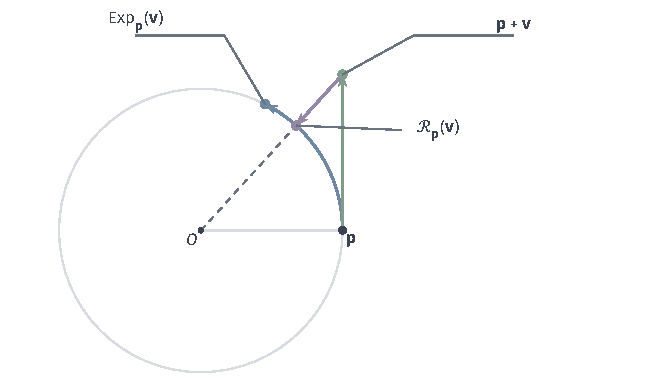
\includegraphics[width=112.0mm]{figures/01-mathematical-preliminaries-upper/02-linear-algebra-and-geometry/tikz/geometry-sphere-retraction/figure.pdf}
  \caption{单位圆截面中的切向步、指数映射与归一化回缩。
 取$\bm p=(1,0)^\top$、$\bm v=(0,1.1)^\top$。箭头为切向步，
 终点$\bm p+\bm v$位于圆外；紫色径向箭头将该点归一化为$\mathcal R_{\bm p}(\bm v)$。
 从起点方向计，蓝色指数更新转过$1.1$弧度，归一化回缩转过
 $\arctan(1.1)\approx0.833$弧度。两种更新关于步长的曲线在零步长处有相同初速度，
 但有限步位置不同。图为解析教学示例。}
 \label{fig:geometry-sphere-retraction}
\end{figure}
\FloatBarrier

\subsubsection{基于Newton与信赖域的二阶求解}
\label{sec:geometry-riemannian-newton-trust-region}

梯度只给局部下降方向，Hessian还能描述不同方向的二阶变化。
在当前点$\bm p$的切空间建立模型
\[
 m_{\bm p}(\bm\eta)=f(\bm p)
  +g(\operatorname{grad}f,\bm\eta)
  +\frac12g(\bm\eta,\operatorname{Hess}f[\bm\eta]).
\]
Newton方向解
$\operatorname{Hess}f[\bm\eta]=-\operatorname{grad}f$，
再用$\mathcal R_{\bm p}(\alpha\bm\eta)$更新。
取切空间正交归一基后，这是已有线性求解方法处理的对称系统；
一般坐标中可用式~\eqref{eq:geometry-hessian-coordinates}写成
$\bm B\bm\eta=-\nabla_{\bm z}f$。
Hessian奇异时方向可能不存在或不唯一，不定时Newton方向也可能不是下降方向。
局部快速收敛需要非退化解、足够光滑性、合适回缩和足够近的初始点，
不是二阶公式本身提供的全局保证。

信赖域方法限制模型适用范围，在$\lVert\bm\eta\rVert_g\leq\Delta$中近似最小化
$m_{\bm p}$。用实际下降与预测下降之比
\[
 \rho=\frac{f(\bm p)-f(\mathcal R_{\bm p}(\bm\eta))}
             {m_{\bm p}(\bm0)-m_{\bm p}(\bm\eta)}
\]
判断接受步和调整$\Delta$，只在分母为正时使用这个比值。
它允许利用负曲率方向，同时避免把远离当前点的模型误当成目标本身。
收敛结论仍需模型误差控制、子问题下降量及更新规则。

这里有一个二阶条件容易遗漏。令拉回目标
$\widehat f_{\bm p}(\bm\eta)=f(\mathcal R_{\bm p}(\bm\eta))$，
它定义在固定向量空间$T_{\bm p}\mathcal M$上。
回缩只保证其零点一阶导数等于$\mathrm df_{\bm p}$。
设$c(t)=\mathcal R_{\bm p}(t\bm\eta)$，由
式~\eqref{eq:geometry-function-second-derivative}，
\begin{equation}
 \frac{\mathrm d^2}{\mathrm dt^2}\widehat f_{\bm p}(t\bm\eta)
 \bigg|_{t=0}
 =g(\bm\eta,\operatorname{Hess}f[\bm\eta])
  +g(\operatorname{grad}f,D\dot c/\mathrm dt|_{t=0}).
 \label{eq:geometry-retraction-pullback-hessian}
\end{equation}
若回缩对所有$\bm\eta$均满足$D\dot c/\mathrm dt|_0=\bm0$，
称为二阶回缩（second-order retraction）。此时，或当前点已经驻定时，额外项才必定消失，
拉回目标的零点Hessian才与Riemann Hessian一致。
指数映射满足该条件；球面归一化回缩也满足，因为
$c''(0)=-\lVert\bm\eta\rVert_2^2\bm p$为纯法向。
对任意一阶回缩直接作二阶等同则不成立，
必须修正模型或另外证明所用模型满足算法的误差要求。
这些模型条件及一阶、二阶算法的收敛分析可参见Boumal的教材\scite{math-boumal2023optimization}。

若算法还复用前一步动量或搜索方向，它们位于旧切空间，不能与当前梯度直接相加。
可以沿已选路径作平行移动，也可指定较便宜的向量搬运（vector transport）
$\mathcal T_{\bm\eta}:T_{\bm p}\mathcal M\to
T_{\mathcal R_{\bm p}(\bm\eta)}\mathcal M$，
要求其对被搬运向量线性、随变量光滑且零步长时为恒等映射。
例如嵌入流形可投影旧方向到新切空间；这一般不保长度，甚至可能压掉某些方向，
并不是Levi--Civita平行移动。采用哪种搬运及它保留什么性质，
必须与具体迭代方法一起说明。

\section{收敛与逼近}
\label{sec:geometry-convergence-approximation}

沿流形取出的点列，首先只涉及极限是否属于原空间；优化迭代还受目标与更新规则支配。
局部线性近似与有限采样又引出另一组问题：切平面、距离和拓扑能否逼近潜在对象？
下面依次规定每项的目标、误差与尺度，避免用点列收敛替代几何恢复。

\subsection{点序列的收敛}
\label{sec:geometry-point-convergence}

点序列$\bm p_n$收敛到$\bm p$，意味着$\bm p$的每个邻域最终包含全部$\bm p_n$。
在包含$\bm p$的坐标图中，这等价于坐标$\chi(\bm p_n)$趋于$\chi(\bm p)$：
坐标图及其逆连续，且序列最终留在该图内。嵌入模型中也等价于环境坐标收敛到属于流形的$\bm p$。
目标点的归属不能省略，例如开单位圆弧中的点可以在环境中趋于被删去的端点，
却不在原空间中收敛。

Riemann距离给出相同的局部拓扑。取$\bm p$附近一个闭包仍在图内的小坐标球，
光滑正定度量的最小、最大特征值在其上分别有正下界和有限上界。
连接近点的坐标线段给出距离上界；任何离开这个小球的路径又必须付出正长度，
留在球内的路径长度则不小于坐标位移乘一个正系数。
所以足够近时坐标收敛与$d_g$收敛相互推出。
距离柯西列只保证点彼此越来越近；每个这样的列都有空间内极限才称完备。
定理~\ref{thm:geometry-hopf-rinow-existence}使用的正是这个条件，而不是坐标图覆盖的大小。

\subsection{点优化下的迭代序列收敛}
\label{sec:geometry-point-iteration-convergence}

回缩梯度法产生的序列还受目标与步长支配。设目标有下界$f_{\inf}$，且被接受的步满足
\[
 f(\bm p^{(k)})-f(\bm p^{(k+1)})\geq
 c\alpha^{(k)}\lVert\operatorname{grad}f(\bm p^{(k)})\rVert_g^2.
\]
求和后有
$\sum_k\alpha^{(k)}\lVert\operatorname{grad}f(\bm p^{(k)})\rVert_g^2
\leq(f(\bm p^{(0)})-f_{\inf})/c$。
若步长有统一正下界，就推出梯度范数趋零；
只知道步长趋零则不能作此推断。
在紧的下水平集上，若回缩光滑且拉回目标有统一的局部二阶界，
每步从同一个正试探步长开始、以固定比例回溯，就能让足够小的步长统一满足下降条件。
回溯会在这一统一尺度内停止，因此被接受的步长有正下界。
这些条件还确保更新留在回缩定义域内。

紧性保证有聚点；梯度连续使每个聚点驻定，却不自动保证所有迭代点趋于同一聚点，
也不把驻点变成全局最优。Newton局部快速收敛与信赖域全局驻点分析
还分别需要非退化性、模型一致性和子问题下降量条件。
因而收敛结论必须针对实际生成的序列陈述，不能由“在流形上使用梯度”单独推出。

\subsection{局部线性表示下的流形逼近}
\label{sec:geometry-local-linear-approximation}

切空间之所以适合近似，由Taylor展开说明。若参数化在当前邻域内二阶导数有界，则
\begin{equation}
 \varphi(\bm z+\bm h)-\varphi(\bm z)
 =\bm J_\varphi(\bm z)\bm h+O(\lVert\bm h\rVert_2^2).
 \label{eq:geometry-manifold-local-taylor}
\end{equation}
一阶项属于切空间，故环境位移投到法向正交补后只剩二阶余项。
这是局部结论，常数依赖所选邻域及二阶导数界；不能将它延伸到任意大步长。
法向偏离反映嵌入在环境中怎样弯曲，不等于第\ref{sec:geometry-riemannian-curvature}节定义的内在曲率。
在二维开带中法向空间为零，弯曲坐标线本身就不构成法向误差。


这里已知的是参数化曲面，用同一点的仿射切平面近似它。
二阶余项随坐标半径平方缩小；它是确定性局部偏差，不是样本协方差的统计误差。
仿射切平面本身可以无限延伸，近似保证却只在当前参数化与余项界有效的小邻域内成立。

\subsection{有限采样下的切空间逼近}
\label{sec:geometry-sampled-local-linearization}

只有$\bm x_i=\bm p_i+\bm\epsilon_i$时，参数化与潜在位置通常未知。
局部PCA（local principal component analysis）用邻域样本最主要的线性变化方向
估计真实切空间，是一种估计方法而不是流形的定义。
必须先说明潜在对象是二维带还是一维中心线，才能确定希望估计什么。

给观测$\bm x_i$选择邻居索引集$N_i$和权重
$\alpha_{i,j}\geq0$、$\sum_{j\in N_i}\alpha_{i,j}=1$，计算
\begin{equation}
 \overline{\bm x}_i=\sum_{j\in N_i}\alpha_{i,j}\bm x_j,\qquad
 \bm C_i=\sum_{j\in N_i}\alpha_{i,j}
  (\bm x_j-\overline{\bm x}_i)(\bm x_j-\overline{\bm x}_i)^\top.
 \label{eq:geometry-local-weighted-covariance}
\end{equation}
若潜在维数$d$给定，取$\bm C_i$最大$d$个特征值对应的正交特征向量
$\widehat{\bm U}_i$，其列空间$\widehat T_i$为估计方向子空间。
若$d$未知，需另由谱和误差模型判断；不能把预先指定的特征向量数当成维数发现。
局部均值消去样本位置偏移，但不保证等于$\bm p_i$。

这里有三个对象。$T_{\bm p_i}\mathcal M$是真实方向，
$\widehat T_i$是以零向量为原点的估计方向，
$\overline{\bm x}_i+\widehat T_i$或$\bm x_i+\widehat T_i$才是画出来的仿射近似。
若$d<D$，一般环境噪声使$\bm x_i\notin\mathcal M$，
此时$T_{\bm x_i}\mathcal M$甚至没有定义。
二维开带是当前例外：小噪声下观测仍在开带内，其切空间仍为$\mathbb R^2$，
但这不表示已经识别出生成它的潜在位置。

式~\eqref{eq:geometry-manifold-local-taylor}解释了误差来源。
在正则局部坐标中，邻域尺度为$h$时，切向位移通常为$O(h)$，
嵌入法向偏离为$O(h^2)$。若采样在各切方向上充分展开，
切向协方差特征值具有$h^2$量级；法向位移的平方贡献则可达到$h^4$量级。
这些尺度比较需要二阶导数有界和非退化局部采样，单靠光滑性并不保证谱间隙。


即使局部方向估计准确，也尚未得到全局坐标。圆的每个邻域只有一个切方向，
却不能以单张无断点实坐标图覆盖。局部PCA提供的是后续几何计算的局部输入，
不是全局展开或任务语义正确性的保证。

\subsection{有限采样下的距离逼近}
\label{sec:geometry-sampled-geodesic-distance}

只有观测点时，常把距离小于阈值$\varepsilon$的点相连，
或连接每个点的$k$个最近邻，再以$\lVert\bm x_i-\bm x_j\rVert_2$为边长。
一条边路径的长度是所经边长之和，最短边路径试图近似所选潜在流形上
$d_g(\bm p_i,\bm p_j)$。这里只借用顶点、边和路径的直观含义，
通用图算法留给第~\ref{part:discrete-mathematics-and-graph-theory}部分。

潜在对象必须先定。若观测不在潜在流形上，$d_g(\bm x_i,\bm x_j)$便未定义；
即使观测在二维开带内，也不能因此把它认作$\bm p_i$。
环境欧氏边长自然对应欧氏诱导度量的局部近似；
若目标采用另一个Riemann度量，就要据此修正边长，不能继续沿用欧氏弦长而声称目标未变。

邻域要小到每条边只跨越近似平直的一段，避免从一折跳到另一折；
又要大到样本间的空隙能够连通。超过跨折环境间隔会引入捷径，低估沿潜在空间的距离；
小于采样空隙则会把一个真实分支拆开，返回无穷距离。
即使没有捷径，局部弦长误差与离散路径绕行误差也会共同作用，
不能无条件断言估计总在真实距离的同一侧。

固定$k$并不固定几何尺度。稀疏处第$k$个邻居可能很远，稠密处则很近，
有向近邻关系还可能不对称，需要声明如何对称化。
一致近似通常要求潜在流形光滑、采样在所研究区域逐渐稠密、
噪声相对邻域尺度受控，并让邻域半径随样本量缩小而仍足以覆盖采样空隙。
非紧开带若只在一部分采样，这些要求也只支持相应覆盖区域的结论。
具体收敛速度须结合采样分布与尺度选择证明，
最短边路径正确更不自动意味着后续全局坐标恢复正确。

\subsection{有限采样下的拓扑逼近}
\label{sec:geometry-sampled-topology-approximation}

固定同一组点和尺度，可以按共同覆盖或成对接近构造复形。
\begin{definition}[Čech复形与Vietoris--Rips复形]
\label{def:geometry-cech-rips-complexes}
给定欧氏点集$\{\bm x_i\}$及$\varepsilon>0$，以
$B(\bm x_i,\varepsilon/2)$表示开球。
\term{Čech复形}（Čech complex）$\mathcal C_\varepsilon$纳入所有满足
$\bigcap_{i\in\sigma}B(\bm x_i,\varepsilon/2)\neq\varnothing$的非空顶点集$\sigma$。
\term{Vietoris--Rips复形}（Vietoris--Rips complex）$\mathcal R_\varepsilon$
纳入所有满足$\lVert\bm x_i-\bm x_j\rVert_2\leq\varepsilon$
对任意$i,j\in\sigma$成立的非空顶点集。
\end{definition}
这两种规则都向下封闭。Čech边要求距离严格小于$\varepsilon$，
Rips边在此采用不超过$\varepsilon$的约定；开闭边界的差异须在临界尺度明确保留。
更本质的差别出现在三点以上：成对相交不保证共同交集。

例如$\varepsilon=1$、边长$0.9$的正三角形，三对半径$0.5$的球均相交，
因此Rips加入三角面。覆盖三个顶点的最小球半径却是$0.9/\sqrt3>0.5$，
不存在三个球的共同交点，Čech只保留三条边。
图~\ref{fig:geometry-cech-rips-intersection}中的中心叉号给出这个最小覆盖半径，
不是利用开闭球的等号差异制造反例。
\begin{figure}[htbp]
  \centering
  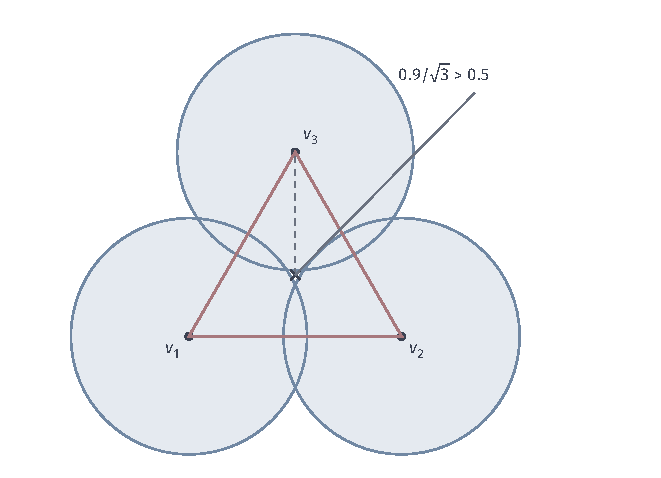
\includegraphics[width=112.0mm]{figures/01-mathematical-preliminaries-upper/02-linear-algebra-and-geometry/tikz/geometry-cech-rips-intersection/figure.pdf}
  \caption{固定同组三点比较共同交集与成对条件。正三角形边长$0.9$，
 $\varepsilon=1$，蓝色开球半径$0.5$；红色边满足两种构造的连边条件。
 三球无共同交点，Čech不含二维面，Rips含二维面。
 中心到各顶点的距离为$0.9/\sqrt3>0.5$。圆周只标开球边界，图为解析教学构造。}
 \label{fig:geometry-cech-rips-intersection}
\end{figure}

尺度变化后仍可给出明确包含关系。对任意$\eta>0$，有
\[
 \mathcal C_\varepsilon\subseteq\mathcal R_\varepsilon
 \subseteq\mathcal C_{2\varepsilon+\eta}.
\]
第一个包含关系由共同交点和三角不等式推出。
对第二个，任选一个顶点作候选共同交点，它到其余顶点的距离至多$\varepsilon$，
严格小于新球半径$\varepsilon+\eta/2$。
若全部球改用闭球，在相应定义下可取尺度常数$2$而不加$\eta$。
这些是足够的普适常数，不声称最紧；同一尺度的复形仍不能互换。

复形何时能代表球并集的拓扑，还依赖覆盖条件。良好覆盖（good cover）要求每个
非空有限交集都可连续收缩到一点；有限欧氏开球的交集为凸集，满足这项要求。
神经引理（nerve lemma）在该条件下说明Čech复形与球并集同伦等价，即二者存在相互映射，
来回复合可以连续变形到恒等映射。这里不要求两映射互为逆，所以比同胚弱：
闭区间可连续收缩到一个点，与单点空间同伦等价，却不可能与它存在双射。
这个结论不等于球并集已经恢复了未知潜在流形；
后者还需要采样覆盖和尺度条件。


复形的规模还依赖邻域尺度。开带$\mathcal M_{\mathrm{strip}}$与开矩形同胚，
中心线$\mathcal C$与开区间同胚，都没有全局环。
闭合中心线得到圆，保留横向自由度并闭合则得到二维环带；
维数不同，但都保留绕中心的一维环。只有在采样和尺度适当时，样本复形才有理由
反映这些区别。尺度太小会把采样空隙误认作分支；太大则可能跨折连边，
并以高阶面填掉原来的环。

持续同调（persistent homology）跟踪随尺度增大而嵌套的复形中，同调类何时出现、
何时消失；它提供跨尺度信息，不使所有长寿命结构自动具有真实任务语义。


硬阈值还会使略跨尺度的一对点从相连突然变为不相连。软关系改用
$\mu_{i,j}\in[0,1]$表示所选局部尺度下的邻接支持强度；
这只是隶属度，不自动是事件概率。高阶强度例如可取全部边强度的最小值，
但必须声明采用哪种规则。一种常见的合并运算是
\begin{equation}
 a\mathbin{\sqcup}b=a+b-ab=1-(1-a)(1-b),\qquad a,b\in[0,1].
 \label{eq:geometry-fuzzy-union}
\end{equation}
结果仍在$[0,1]$内；交换性由对称式给出，结合性由
$1-(1-a)(1-b)(1-c)$给出，$0$为恒等元，任一输入为$1$时输出为$1$。
这些性质使它成为明确定义的软并集，却没有提供独立事件的随机试验或联合分布。
核权重、相似度、置信度与概率的校准要求不能仅凭数值范围混同。

UMAP等方法由局部距离构造带强度的关系，再优化低维坐标以匹配这些关系；
具体目标与优化过程留给
\BookChapterRef{chap:dimensionality-reduction}{卷4《模型：经典模型》第5章“降维”}。
低维图像中的分离簇或孔洞还可能受邻居数、尺度、初始化与优化误差影响。
拓扑方法不能修复错误的局部输入：跨折捷径会被忠实组合，完全漏采的区域也无法凭空
恢复。采样覆盖、局部关系与尺度共同限制结论。

\section{扰动与稳定性}
\label{sec:geometry-stability}

缩小邻域或增加采样，改变的是逼近条件；观测稍变以后输出会变多少，则是稳定性问题。
以下分别比较映射输出、估计切空间、重构坐标与拓扑，以及路径解。
比较方向时先消去基的任意性，比较坐标时先消去距离无法识别的刚性变换，
才能把真正的响应与记录差异分开。

\subsection{运算的误差传播}
\label{sec:geometry-operation-stability}

对光滑点映射$F$，记其局部坐标表达为$\widehat F$。
在一个凸坐标区域上设$\lVert\bm J_{\widehat F}\rVert_2\leq L$，
沿区域内的线段积分得到
$\lVert\widehat F(\bm z+\bm h)-\widehat F(\bm z)\rVert_2
\leq L\lVert\bm h\rVert_2$。
跨图时还需计入两端坐标转换及度量的上下界；一个坐标中的小扰动不是坐标无关的数值。
叠加的局部放大界不超过$\sum_j|a_j|L_j$，复合不超过各步界的乘积。
若归一化分母趋零、参数化Jacobian接近降秩，这些界会变差，
因此合法运算与数值稳定是两个需要分别核对的条件。

\subsection{切空间估计的稳定性}
\label{sec:geometry-tangent-estimate-stability}

局部PCA从协方差矩阵选出一个子空间。因此，先比较理想与实际协方差，
再用上一章的子空间扰动结论把矩阵误差转成方向误差：
当$d<D$时，若理想局部协方差在第$d$与第$d+1$特征值间有间隙$\delta>0$，
而观测造成的算子范数扰动相对$\delta$足够小，则估计子空间的偏转受
$\lVert\bm E\rVert_2/\delta$控制。这里$\bm E$要包括有限样本波动、
噪声、邻域错选及非线性近似误差，不能只代入测量噪声方差。
若已知$d=D$，目标切空间就是整个环境空间$\mathbb R^D$，
无需用这条谱隙辨认方向；维数是否确为$D$仍是另一个模型判断。

缩小邻域会降低法向二阶偏差，却减少样本并压低真实信号的谱尺度；
固定噪声不会随之自动消失。邻域过大时，中心线不同位置的切线已明显转动，
PCA得到的是折中方向。对二维窄带，若样本的横向覆盖不足或宽度小于噪声尺度，
第二个方向可能难以稳定识别，但潜在对象并不因此变成一维。
固定近邻数也不能解决非均匀密度带来的变化：稀疏处覆盖范围大，稠密处范围小。
潜在对象、采样密度、嵌入弯曲、邻域尺度、谱间隙和噪声必须一起解释。


估计子空间内部的基可以旋转，输出应比较投影或主角，而不是逐列比较特征向量。
谱隙、邻域尺度和噪声一起决定能否区分切向与法向；增加样本数量不能消除固定尺度带来的几何偏差。

\subsection{坐标重构的稳定性}
\label{sec:geometry-coordinate-reconstruction-stability}

设平方距离矩阵由$\bm\Delta$变成$\bm\Delta+\bm E$。
中心化矩阵$\bm J$是正交投影，故重构Gram矩阵的扰动为
\[
 \widetilde{\bm B}-\bm B=-\tfrac12\bm J\bm E\bm J,\qquad
 \lVert\widetilde{\bm B}-\bm B\rVert_2\leq\tfrac12\lVert\bm E\rVert_2.
\]
第\ref{sec:linear-algebra-spectral-stability}节的谱扰动结论控制特征值与选定谱子空间。
选取前$d$维坐标时，需要$d$与$d+1$模态之间的谱隙；
对正特征值开平方还需要它们远离零。接近零的模态可能改变保留维数，
重复特征值则允许同一子空间内任意转动。

比较坐标前应先消去平移，再允许整体正交对齐，因为距离本来就不识别这些变换。
若点标签也改变，还须先建立点对应。小距离扰动只能在上述尺度与对齐条件下
支持坐标稳定，不能保证某个优化过程恰好返回同一朝向的坐标。

\subsection{拓扑重构的稳定性}
\label{sec:geometry-topology-reconstruction-stability}

固定阈值构造的单个复形可能发生跳变。若成对距离误差不超过$\delta$，
所有距离原本小于$\varepsilon-\delta$的边仍会被纳入，
原本大于$\varepsilon+\delta$的边仍会被排除；处在中间带内的边不能保证。
对Rips复形，这直接给出
$\mathcal R_{\varepsilon-\delta}\subseteq\widetilde{\mathcal R}_{\varepsilon}
\subseteq\mathcal R_{\varepsilon+\delta}$（左侧只在正尺度使用）。
固定尺度上的Betti数仍可能变化；跨尺度比较能把不确定性记录为尺度偏移，
但具体持续图距离的界还需要所用过滤的稳定性定理。
完全漏采的区域、错误点对应或大幅跨折连边并不属于小扰动假设，
不能从局部稳定性恢复其中的信息。

\subsection{路径解的稳定性}
\label{sec:geometry-path-solution-stability}

初值问题同时更新位置与速度。把状态记为$\bm y=(\bm z,\dot{\bm z})$以后，
它在一张坐标图中成为一阶系统$\bm y'=A(\bm y)$；
$A$由测地线方程中的速度与加速度组成。
设另一方程为$\widetilde{\bm y}'=\widetilde A(\widetilde{\bm y})$。
若两条解留在同一紧区域$K$，$A$在该区域有Lipschitz常数$L$，
且$\sup_{\bm y\in K}\lVert A(\bm y)-\widetilde A(\bm y)\rVert\leq\eta$，
积分方程给出
\[
 \lVert \bm y(t)-\widetilde{\bm y}(t)\rVert
 \leq e^{Lt}\lVert \bm y(0)-\widetilde{\bm y}(0)\rVert
       +\eta\int_0^t e^{L(t-s)}\,\mathrm ds,\qquad t\geq0.
\]
这是Gronwall不等式的直接应用，比较的是固定时间区间上的初值轨迹。
一旦路径离开该区域，常数与比较图都须重新核对。

固定端点的最短路有不同边界：距离作为最小代价可能连续，
达到它的路线却未必唯一。球面上到对跖点的最短路有多条；
终点向不同方向稍微偏离，会选出不同的大圆弧。
若局部有唯一最短路且避开使端点映射退化的位置，才可利用指数映射的局部逆
控制路线对端点的响应。初值唯一性不能替代端点最短路的稳定性条件。

\section{本章小结}
\label{sec:geometry-summary}

本章把非线性对象的局部记录、关系、运算、求解、逼近与稳定性分开建立。
坐标图记录位置，切空间规定瞬时方向，度量读出长度，路径长度的下确界定义距离；
等价关系则明确哪些输入变化被主动忽略。局部自由度、环境维数和有限观测不是同一对象。

映射微分传递速度，联络与平行移动比较不同位置的方向，指数映射和回缩产生可行的新点。
给定初值求轨迹与给定端点求最短路有不同的唯一性、存在性和稳定性边界。
点优化调用这些运算选择更新，其下降、驻点与点序列收敛仍须分别证明。

局部切平面、样本PCA、最短边路径和复形各自逼近方向、距离或拓扑。
尺度、覆盖、谱隙与噪声决定适用范围；环境弯曲、内在曲率和整体孔洞不能互相替代。
下一章把整个函数作为可变对象，沿用这里的几何域、微分与体积，
研究函数读取、函数拟合以及平滑能量所决定的函数与场优化。

\chapter{函数空间}
\label{chap:functional-analysis-and-approximation}

\newcommand{\functionalinlinetablecaption}[2]{%
  \refstepcounter{table}\label{#1}%
  \addcontentsline{lot}{table}{\protect\numberline{\thetable}#2}%
  \par\smallskip\noindent
  {\figurefont\footnotesize
   \textcolor{BookTeal}{表~\thetable}\quad #2}\par}
\newcommand{\functionalinlinefigurecaption}[2]{%
  \refstepcounter{figure}\label{#1}%
  \addcontentsline{lof}{figure}{\protect\numberline{\thefigure}#2}%
  \par\smallskip\noindent
  {\figurefont\footnotesize
   \textcolor{BookTeal}{图~\thefigure}\quad #2}\par}

把一条曲线或一个多变量函数当作整体来看待时，有限维几何里那一套“点、长度、投影、微分”仍然能提供很好的起点，却不能直接照抄。一个输入坐标并不意味着候选函数只有一个变化方向；有限几个读数也不自动确定整条函数；一个看起来漂亮的无穷展开，未必在某种整体误差下收敛。本章要处理的，正是把“函数本身”作为一个元素以后，必须重新回答的几个问题：哪些函数允许参与运算，怎样衡量两条函数之间的整体偏差，怎样合法地读取或变换一条已知函数，又怎样根据观测和目标去确定、逼近一条未知函数。

先用一个熟悉的情形说明问题出在哪里。拟合曲线时，有限维模型常把函数写成固定基函数的线性组合
\begin{equation}
  f_m(x)=\sum_{j=1}^{m}a_j\varphi_j(x).
  \label{eq:functional-finite-basis-expansion}
\end{equation}
当$m$固定时，可以把系数$(a_1,\ldots,a_m)^{\top}$当作普通向量，用欧氏距离比较两个候选解。可是一旦允许基函数数目增加，系数向量所在的维数也随之改变；同一个函数还可能在不同基下拥有完全不同的系数。此时，仅比较参数向量已经不能稳定地回答“两条函数相差多少”“有限表示能否逼近目标”以及“有限观测究竟确定了哪些函数方向”。

有限维经验在这里会遇到三类它独自回答不了的问题。其一，一条信号或曲线的记录数不是固定的：为提高精度可以不断增加基函数个数，“参数有多少个”本身会随表示规模变化，用系数向量的维数比较两条函数不再可靠。其二，许多函数只能描述成“与某条参考函数在几乎每个输入处相差多少”，这时比较的是两个无穷维对象的整体差距，而不是有限个坐标差。其三，无穷个基方向的展开是否收敛、截断多少项才够、某一点的值能否稳定读取，都没有有限维结论可以自动继承。

本章的安排正是围绕这些问题展开。第~\ref{sec:function-spaces-and-norms}节先把函数作为元素，建立范数与误差之间的关系；第~\ref{sec:weak-derivatives-sobolev}节在允许弱导数的条件下构造Sobolev空间。这两节提供后续共用的对象和结构。主体任务随后分别展开：第~\ref{sec:linear-readouts-orthogonal}节研究怎样读取函数信息并作正交表示，第~\ref{sec:linear-operators-integral-equations}节研究线性算子与积分方程，第~\ref{sec:variational-functional-fitting}节以观测和目标确定未知函数，第~\ref{sec:finite-representation-approximation}节为给定目标设计有限表示，第~\ref{sec:discrete-energy-approximation}节用有限采样表达已知函数的能量，第~\ref{sec:covering-numbers}节衡量整个函数类需要多少近似代表。这些小节按当前所求对象和操作目标分工，空间名称与算法名称并不当作互斥的类别。

需要先说明“收敛”和“稳定”这两个词在本章的含义随对象而变：正交截断是在增加保留的方向数，积分方程迭代是在增加计算次数，正则化是在改变目标参数，数据扰动则是重新求解另一个任务的解。因此相应的条件和估计都放在各自任务中讨论，不用一个不指明对象的“收敛”或“稳定”笼统代替。单个函数的逼近误差、固定记录的能量值、整个函数类的覆盖数，也分别给出各自的误差与量词。具体的场方程与几何结构则留给后续的微分方程和流形章节。

本章主要讨论实值函数与实Hilbert空间；遇到向量值函数时按分量处理。需要强调的是，对输入位置$x$求导描述的是函数自身的空间变化，而把整条未知函数当作变量作扰动，描述的则是目标如何评价候选的变化，这两类“微分”贯穿全章但始终分开。

\section{函数空间与范数}
\label{sec:function-spaces-and-norms}

把整条函数作为一个元素时，要先确定哪些函数允许参与线性运算、哪些差异算作同一个元素，再选择衡量整体偏差的规则。本节先把这项共同准备与具体范数构造分开：第~\ref{subsubsec:norm-inner-product-completeness}节建立函数元素、范数、内积与完备性等共用概念；第~\ref{subsec:constructing-function-norms}节具体构造最大偏差范数与积分范数；第~\ref{subsec:comparing-spaces-errors}节再比较不同空间、不同测度以及不同误差规则之间的关系。Banach、Hilbert与$L^p$各自表达的是不同条件，并不作为互斥类型并列。

\subsection{函数元素与空间结构}
\label{subsec:function-elements-structure}

本小节先说明空间收进什么对象，再说明要在这些对象上增加哪些结构。普通函数和几乎处处等价类的区别决定零元素如何识别；线性运算、范数、内积与完备性则分别承担组合、计量和取得极限的职责。

\subsubsection{线性空间与函数元素}
\label{subsubsec:linear-function-candidates}

同一输入集合上的函数可以逐点相加和缩放；但预先限定的候选族是否容纳这些结果，还要逐一检查。有测度时，还必须决定是否保留每个位置上的取值差异。

\paragraph{函数的线性运算与候选范围}

固定一个非空输入集合$X$，先以实值函数$f:X\to\mathbb R$为主线，并注意区分三个层次的对象：自变量$x$、$x$处的标量值$f(x)$，以及整个函数$f$。逐点定义加法和数乘
\[
  (f+g)(x)=f(x)+g(x),\qquad (cf)(x)=c\,f(x),
\]
这些运算由实数上的相应运算逐点继承，因而全体函数$X\to\mathbb R$满足线性空间的全部公理。取有限维向量值函数$f:X\to\mathbb R^r$时，按分量定义相同运算即可。

从全体函数缩小到某个候选族$V$时，不能只凭“它由若干函数组成”就称$V$为线性子空间，而要逐项检查零函数是否在其中、两个成员之和是否仍在其中、成员的标量倍是否仍在其中。连续函数族满足这些要求：两个连续函数相加或数乘后仍连续，零函数也连续；有限个生成函数$\varphi_1,\ldots,\varphi_m$的线性张成$\operatorname{span}\{\varphi_j\}$同样如此。作为对照，固定节点预算的一般非线性参数族未必封闭：两个各用$N$个节点的成员相加，可能需要多于$N$个节点才能表示，因此参数形式本身不保证线性封闭。

还要区分三个容易混淆的“维数”：输入域的维数、表示参数的数目、函数空间的维数。即使输入域只是实轴或一个非退化区间（输入维数为一），函数$1,x,x^2,\ldots$仍能提供任意多个线性无关的方向。固定深度的网络若要并行表示两个网络之和，通常必须增加宽度或节点预算，不能从“输入只有一个坐标”或“深度固定”推出候选空间有限维。把空间的成员范围固定下来以后，才进入“同一成员如何识别”的问题。

\paragraph{普通函数与几乎处处等价类}

对普通函数采用的是逐点相等：某个位置的值一旦改变，就得到不同的函数。但若误差是通过测度积分累计的，在零测集上的修改可能完全不改变误差。承接第~\ref{chap:univariate-calculus}章建立的零测集与几乎处处概念，我们需要另一种元素识别方式，记作
\[
  f\sim_\mu g\quad\Longleftrightarrow\quad f=g\text{ 在$\mu$下几乎处处成立}.
\]

在可测函数中以$[f]_\mu$表示这个等价类。加法和缩放不依赖代表的选择：若$f$换成与之几乎处处相同的$f'$，$g$换成$g'$，那么$f'+g'$与$f+g$、$cf'$与$cf$不同的位置只是两个零测集的并，仍然是零测集。这里用到的依据来自前章已由测度可数次可加性证明的结论：可数个零测集的并仍是零测集；两次换代表的例外集取有限并后仍为零测，这就保证运算结果仍几乎处处相同。于是
\[
  [f]_\mu+[g]_\mu=[f+g]_\mu,\qquad c[f]_\mu=[cf]_\mu
\]
都是良定义的。本小节只建立后面积分空间共用的对象约定；$L^p$和$L^\infty$各自的成员条件和范数要到具体构造处才定义。

零函数与“仅在一个Lebesgue零测单点取一、其余处取零”的函数是说明这一区别的最简例子：作为普通函数它们不同，作为等价类却相同。前章已从简单函数积分以及非负函数的逐段逼近证明，零测修改不影响积分；每个单点质量为零，并不使$[0,1]$上常数一的积分变成零，因为可列可加性不能被改成“不可数个单点直接求和”。这个区别目前只处理元素识别；至于某一点的值能否读取，要等到域内点值读取那一节另行判断。

图~\ref{fig:vol1-add-functional-ae-representatives}把“函数不同”与“积分空间中的元素相同”分开。绿色孤立读数不会改变Lebesgue积分，所以这两条代表在$L^p$中距离为零，但在该位置的函数值仍不同。
\begin{figure}[!htb]
  \centering
  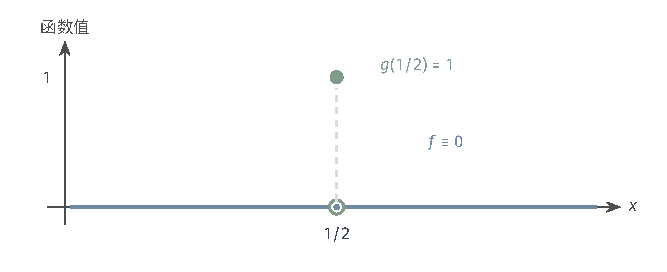
\includegraphics[width=112mm]{figures/01-mathematical-preliminaries-upper/02-linear-algebra-and-geometry/tikz/comprehension-additions/functional-ae-representatives.pdf}
  \caption{同一积分元素的不同代表。定义域为$[0,1]$并用Lebesgue测度，$f\equiv0$，$g$除$g(1/2)=1$外也为零。绿空心圈表示$g$不在该点取零，圈内蓝点保留$f(1/2)=0$。单点集合测度为零，故任意$1\le p<\infty$下$\|f-g\|_{L^p}=0$；点值读取却不同。}
  \label{fig:vol1-add-functional-ae-representatives}
\end{figure}

\subsubsection{范数、内积与完备性}
\label{subsubsec:norm-inner-product-completeness}

候选及元素相等的含义确定以后，误差公式还必须满足相应公理，极限过程也必须能在同一空间内完成。本节先把范数、Banach条件和Hilbert条件各自要回答的对象与条件说清，后面的具体空间再据此逐一核验。

\paragraph{范数与函数距离}

要比较$f$与$g$的整体偏差，自然的做法是先为单个函数确定“大小”，再由差$f-g$得到两函数之间的距离。在已经确定元素识别的实线性空间$V$上，范数是一个映射$\|\cdot\|:V\to[0,\infty)$，满足三条要求
\begin{align*}
  &\|f\|=0\ \Longleftrightarrow\ f=0,\\
  &\|cf\|=|c|\,\|f\|,\\
  &\|f+g\|\le\|f\|+\|g\|.
\end{align*}
这三条分别保证零误差能被准确识别、按常数缩放时误差一致，以及两段误差合起来不超过各自之和，最后一条就是\term{三角不等式}。令
\[
  d(f,g)=\|f-g\|,
\]
便能把范数公理逐项转成度量公理，从而可以直接回用第~\ref{chap:function-limits}章关于度量空间中柯西列与完备性的结论。需要强调，如果某个公式在普通函数上只能让非零函数长度为零，就必须先处理这些零方向或改用等价类，不能直接宣布它在原候选上是范数。

同一对函数可以用不同范数衡量：有的强调最大偏差，有的强调积分累计，选哪一种取决于当前真正要控制的误差。这里先建立公理与用途；具体公式是否有限、是否满足三角不等式、能识别何种零元素，分别在下一小节核验。

\paragraph{范数空间的完备性与Banach空间}

对范数空间中的一个柯西列，要区分两件事：“各项彼此越来越接近”与“在候选空间内确实存在一个极限”。若每个范数柯西列都存在$V$中的范数极限，就称$V$为\term{Banach空间}。完备性这个条件同时包含所选候选和所选范数，不能只给出一个误差公式就把完备性视为当然。

后面证明具体空间完备时，都会遵循同一条路线：先构造一个候选极限，再证明它保留了该空间的成员条件，最后证明范数误差趋于零。在无限维情形，子空间是否闭、有界列能否抽出范数收敛子列、线性映射是否连续，都必须分别验证，这些性质并不因线性运算成立就自动继承。这里先列清判断边界，后面的投影、读取和算子问题再使用各自的条件。

\paragraph{内积及Hilbert空间}

当任务还要比较函数方向、正交分量或平方误差时，需要在实线性空间上引入内积$\langle f,g\rangle$，要求它对两个变量都是双线性的、对称的，并且$\langle f,f\rangle\ge0$、仅在$f=0$时为零。由
\[
  \|f\|=\sqrt{\langle f,f\rangle}
\]
得到长度。这条长度确实满足三角不等式：对任意实数$t$，
\[
  0\le\|f-tg\|^2=\|f\|^2-2t\langle f,g\rangle+t^2\|g\|^2
\]
是关于$t$的非负二次式，故其判别式不大于零，
\[
  |\langle f,g\rangle|\le\|f\|\|g\|,
\]
即Cauchy--Schwarz不等式；再由
\[
  \|f+g\|^2=\|f\|^2+2\langle f,g\rangle+\|g\|^2
  \le(\|f\|+\|g\|)^2
\]
得到三角不等式。

在这个诱导范数下完备的内积空间称为\term{Hilbert空间}，因此Hilbert空间同时也是Banach空间。一般范数未必来自内积，“是否存在内积”与“是否完备”是两个不同的判断。后面的$L^2$、$W^{k,2}$以及正交读取都会注明使用的是哪个内积、完备性从哪里取得。还要提醒一句，内积给出的是函数空间中的正交关系，并不是两条函数图像在平面中相交的几何角度；图~\ref{fig:vol1-add-functional-integral-orthogonality}正好说明这一点。

\begin{figure}[!htb]
  \centering
  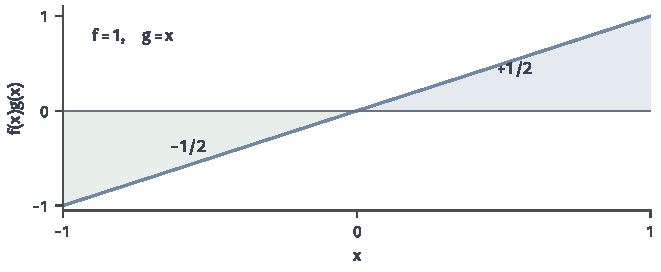
\includegraphics[width=112mm]{figures/01-mathematical-preliminaries-upper/02-linear-algebra-and-geometry/matplotlib/comprehension-additions/functional-integral-orthogonality.pdf}
  \caption{整函数的正交由内积决定。在$[-1,1]$上用Lebesgue积分内积，取$f(x)=1$、$g(x)=x$。图中曲线是乘积$f(x)g(x)=x$，右侧蓝色区域积分为$1/2$，左侧绿色区域积分为$-1/2$，相加为零。因此两函数正交，所画曲线的平面倾角不承担函数空间夹角的含义。}
  \label{fig:vol1-add-functional-integral-orthogonality}
\end{figure}

\subsection{函数范数的构造}
\label{subsec:constructing-function-norms}

固定一对函数后，按偏差的汇总规则可以分为最大偏差控制和积分累计两类。前者再区分处处控制与允许零测例外的控制，后者固定有限的$p$次累计。每种构造都要说清成员、零元素和极限归属，不把具体空间名称当成互斥类别。

\subsubsection{上确界范数}
\label{subsubsec:supremum-norm}

比较两条曲线时，最大偏差控制要求对允许的全部位置给出一个共同上界。普通函数逐点识别与几乎处处等价类的识别不同，因此一致范数和本质上确界范数要分别构造，不能用一个代表的普通上确界代替等价类的本质上界。

\paragraph{连续函数的一致范数}

固定紧区间$[a,b]$上的实连续函数空间$C([a,b])$。为了同时控制所有位置的偏差，定义
\[
  \|f\|_\infty=\sup_{x\in[a,b]}|f(x)|,\qquad d_\infty(f,g)=\|f-g\|_\infty.
\]
连续性与紧性保证这个上确界有限。范数公理逐条成立：$\|f\|_\infty=0$意味着连续函数$f$在每一点为零，即$f=0$；齐次性由逐点缩放后取上确界直接得到；三角不等式由$|f(x)+g(x)|\le|f(x)|+|g(x)|\le\|f\|_\infty+\|g\|_\infty$对每个$x$成立、再取上确界得到，整个函数便成为范数空间中的一个元素。

取一致范数下的一个柯西列$(f_n)$。固定$x$后，
\[
  |f_n(x)-f_m(x)|\le\|f_n-f_m\|_\infty,
\]
所以右边的标量序列是柯西列，由实数完备性逐点定义$f(x)=\lim_n f_n(x)$。这一步只是构造出候选极限，还没有证明一致收敛或连续性。

一致收敛由共同误差界取得：给定$\varepsilon>0$，取$N$使$n,m\ge N$时$\|f_n-f_m\|_\infty<\varepsilon$；对固定的$x$与$n\ge N$，令$m\to\infty$，由绝对值连续得
\[
  |f_n(x)-f(x)|\le\varepsilon,
\]
该界不依赖$x$，故$\sup_x|f_n(x)-f(x)|\to0$。这一步把逐点构造提升为统一误差控制，是证明极限留在空间内的中间环节。

再固定位置$x_0$，把$|f(x)-f(x_0)|$拆成两端的$f-f_N$误差与中间的$f_N(x)-f_N(x_0)$：先选$N$使两端统一地小于$\varepsilon/3$，再利用$f_N$的连续性选择邻域使中间一项也小于$\varepsilon/3$，三项相加得$|f(x)-f(x_0)|<\varepsilon$，便得到$f$连续。因此极限仍留在$C([a,b])$，与上一步合起来才完成Banach性质的证明。

若输入域不紧，连续函数可能无界，普通上确界便可能为无穷；这时要改选有界连续函数空间或另加增长条件。下一项保持最大偏差的汇总规则，只改变零测例外的约定，而不把输入域不紧的问题误当成本质上界的定义理由。

\paragraph{本质上确界范数}

在测度空间$(X,\mathcal A,\mu)$上，积分任务允许忽略零测集，因此从可测实函数的几乎处处等价类出发，定义
\[
  \|[f]_\mu\|_{L^\infty(\mu)}
  =\inf\{M\ge0:|f|\le M\text{ 在$\mu$下几乎处处成立}\},
\]
以该值有限者构成$L^\infty(\mu)$。\term{本质上确界}不随代表变化：若$g$与$f$几乎处处相等，每个使$|f|\le M$成立的零测例外集与$\{f\neq g\}$取并后仍为零测集，同一$M$也控制$g$；但同一等价类各代表的普通上确界可能差别很大。

范数公理逐项核对。正定性：若$\|f\|_\infty=0$，则对每个正整数$k$都有$|f|\le1/k$几乎处处；这些可测例外集的可数并为零测集，其外$|f|\le1/k$对所有$k$同时成立，故$f=0$几乎处处。齐次性由$|cf|=|c||f|$逐点成立直接得到。三角不等式：若$|f|\le C$在零集$N_f$外成立、$|g|\le D$在零集$N_g$外成立，则在$X\setminus(N_f\cup N_g)$上$|f+g|\le C+D$，例外集仍为零测集，故$\|f+g\|_\infty\le C+D$；对$C,D$各自取下确界，得到$\|f+g\|_\infty\le\|f\|_\infty+\|g\|_\infty$。

完备性证明要小心处理例外集。取$L^\infty$柯西列并选可测代表$f_n$。每项几乎处处有界给出可测零集$N_n^0$，使$|f_n|\le M_n$于$X\setminus N_n^0$；柯西性给出：对每个$n,m$与每个正整数$r$，
\[
  |f_n-f_m|\le\|f_n-f_m\|_\infty+\tfrac1r
\]
几乎处处成立，例外集记为$N_{nmr}$。前章已证明可数个零测集的并仍是零测集，故
\[
  N=\left(\bigcup_n N_n^0\right)\cup\left(\bigcup_{n,m,r\in\mathbb N}N_{nmr}\right)
\]
是单一可测零集。在$X\setminus N$上所有不等式对所有下标同时成立，令$r\to\infty$后，所有需要的差值界便同时成立。不能为每个位置各选一个例外集。

在这个共同补集上，范数柯西性给出了真正的一致柯西性。先固定一项$f_1$的有界控制；柯西列$\{\|f_n-f_1\|_\infty\}$有界，设其上界为$C$，则
\[
  |f_n(x)|\le|f_1(x)|+|f_n(x)-f_1(x)|\le M_1+C,\qquad x\in X\setminus N,
\]
故逐点极限$f(x)=\lim_n f_n(x)$在$X\setminus N$上存在且一致有界；在$N$上补零，并由逐点极限与可测零集改值的可测性，$f$是可测代表且$f\in L^\infty$。把共同柯西界的一端送到极限：对$x\in X\setminus N$，
\[
  |f_n(x)-f(x)|=\lim_{m\to\infty}|f_n(x)-f_m(x)|
  \le\limsup_{m\to\infty}\|f_n-f_m\|_\infty,
\]
这在零集$N$之外成立，故$\|f_n-f\|_\infty\le\limsup_m\|f_n-f_m\|_\infty\to0$。于是得到本质上确界范数收敛以及极限的有限本质上界，从而证明$L^\infty$完备。零测修改不改变元素，仍不回答某一指定点值是否确定——这项读取问题要交给后面的点值良定义性处理。

\subsubsection{积分范数}
\label{subsubsec:integral-norms}

若总体偏差按测度累计，就要先选定$p$次累计以及有限积分的成员，再证明范数性质和完备性。下列三个有标题的单元分别负责对象构造、误差公理和空间内极限，不把证明中的每个临时步骤另升成标题。

\paragraph{$L^p$空间及其范数}

固定测度空间与$1\le p<\infty$，从满足
\[
  \int_X|f|^p\,\mathrm d\mu<\infty
\]
的可测实函数出发，按几乎处处相等取等价类。以这些等价类组成$L^p(\mu)$；零积分差识别的是同一等价类，而不是每个位置的值都相同。为了使整体缩放$f\mapsto cf$对应误差乘$|c|$，定义
\[
  \|[f]\|_p=\left(\int_X|f|^p\,\mathrm d\mu\right)^{1/p},
\]
并核对换代表不改变数值：前章已证明零测集上的改动不改变勒贝格积分。$p=1$累计绝对偏差，$p=2$累计平方偏差后开方，一般的$p$改变对大偏差的计价，公式的用途先于不等式证明说明。下文常用代表元$f$代写等价类$[f]$，并简记范数为$\|f\|_p$。

在$[0,1]$的Lebesgue测度下取$f_n(x)=x^n$，可算得
\[
  \|f_n\|_p=\left(\int_0^1x^{np}\,\mathrm dx\right)^{1/p}
  =\left(\frac{1}{np+1}\right)^{1/p}.
\]
它的逐点极限在$x<1$时为零、在$x=1$时为一，仍代表零积分元素；而普通一致范数恒为一。这个例子同时区分了普通函数极限、积分等价类和最大偏差，后面比较各种收敛时只回用这里的计算结果。

现有公式还没有自动保证三角不等式与空间完备性。先用
\[
  |f+g|^p\le 2^{p-1}(|f|^p+|g|^p)
\]
说明成员对加法封闭：逐点有
\[
  (a+b)^p\le(2\max\{a,b\})^p=2^p\max\{a^p,b^p\}\le2^{p-1}(a^p+b^p),
\]
积分后即知$f,g\in L^p$时$f+g\in L^p$。有限$p$与前面的$L^\infty$构造始终保持各自条件。

\paragraph{Hölder不等式与范数性质}

对$1<p<\infty$固定共轭指数$q=p/(p-1)$，则$1/p+1/q=1$。先证明标量Young不等式：对$a,b\ge0$，
\[
  ab\le\frac{a^p}{p}+\frac{b^q}{q}.
\]
固定$b\ge0$，考虑关于$s\ge0$的函数$F(s)=s^p/p-bs$。其导数$s^{p-1}-b$在$s_*=b^{1/(p-1)}=b^{q/p}$处为零，且$F''(s)=(p-1)s^{p-2}>0$，故该处取最小值；代入得$F(s_*)=-b^q/q$，于是$F(s)\ge-b^q/q$对所有$s\ge0$成立，取$s=a$即得Young不等式。

对非零且有限范数的函数，在Young不等式中取
\[
  a=\frac{|f|}{\|f\|_p},\qquad b=\frac{|g|}{\|g\|_q},
\]
积分并复用前章积分的线性与单调性，得到
\[
  \frac{1}{\|f\|_p\|g\|_q}\int_X|fg|\,\mathrm d\mu
  \le\frac{1}{p\|f\|_p^p}\int_X|f|^p\,\mathrm d\mu
  +\frac{1}{q\|g\|_q^q}\int_X|g|^q\,\mathrm d\mu
  =\frac1p+\frac1q=1,
\]
再恢复尺度，得到Hölder不等式
\[
  \int_X|fg|\,\mathrm d\mu\le\|f\|_p\|g\|_q.
\]
若$\|f\|_p=0$，由前章零积分判别定理（$\int|f|=0$当且仅当$f=0$几乎处处）知$fg=0$几乎处处，不等式为平凡$0\le0$；端点$L^1$与$L^\infty$的配对直接由$|fg|\le|f|\|g\|_\infty$积分估计。

已知$f+g\in L^p$后，\term{Minkowski不等式}按如下推导。先由$|f+g|^p=|f+g|^{p-1}|f+g|\le|f+g|^{p-1}(|f|+|g|)$，把$\int|f+g|^p$写成
\[
  \int_X|f+g|^{p-1}|f|\,\mathrm d\mu
  +\int_X|f+g|^{p-1}|g|\,\mathrm d\mu.
\]
两项分别对$|f+g|^{p-1}$与$|f|$、$|g|$应用Hölder。由$(p-1)q=p$，
\[
\begin{aligned}
  \int_X|f+g|^{p-1}|f|\,\mathrm d\mu
  &\le\left(\int_X|f+g|^{(p-1)q}\,\mathrm d\mu\right)^{1/q}\|f\|_p\\
  &=\left(\int_X|f+g|^p\,\mathrm d\mu\right)^{1/q}\|f\|_p,
\end{aligned}
\]
第二项同理，合并得
\[
  \int_X|f+g|^p\,\mathrm d\mu
  \le\left(\int_X|f+g|^p\,\mathrm d\mu\right)^{1/q}
  \bigl(\|f\|_p+\|g\|_p\bigr).
\]
若$\|f+g\|_p>0$，两端同除$(\int|f+g|^p)^{1/q}$，利用$p-p/q=p(1-1/q)=p/p=1$，便得到\term{Minkowski不等式}
\[
  \|f+g\|_p\le\|f\|_p+\|g\|_p.
\]
若$\|f+g\|_p=0$，$f+g$为零等价类，不等式平凡成立。零值情形必须单独落下，不能略过约去项所需的条件。$p=1$时直接对绝对值的逐点三角不等式积分，与前两段合起来完成所有有限$1\le p<\infty$的范数性质。两点计数测度下取两个不相交的单位向量可以看出范围$p\ge1$的实际作用：当$0<p<1$时，两者之和的$p$次累计根为$2^{1/p}>2$，同一公式在该范围不满足范数\term{三角不等式}。

对$p=2$给出
\[
  \langle f,g\rangle=\int_Xfg\,\mathrm d\mu,
\]
由Hölder保证积分存在，逐项核对它是实内积并识别其诱导范数。此时只得到内积结构；等下一单元的完备性完成后，才能据此称$L^2$为Hilbert空间。

\paragraph{$L^p$空间的完备性}

对$L^p$柯西列$(f_n)$，依次选取子列$(f_{n_k})$使
\[
  \sum_k\|f_{n_{k+1}}-f_{n_k}\|_p<\infty.
\]
之所以能选出这样“快速缩小相邻差”的子列，是柯西条件的直接推论：递归取$n_k$，使$n,m\ge n_k$时$\|f_n-f_m\|_p<2^{-k}$。选好子列后再取可测代表，不能把整个原列的逐点收敛当成前提。

对有限部分和
\[
  S_m=|f_{n_1}|+\sum_{k=1}^{m}|f_{n_{k+1}}-f_{n_k}|
\]
使用Minkowski不等式，得到与$m$无关的有限范数上界：
\[
  \|S_m\|_p\le\|f_{n_1}\|_p+\sum_{k=1}^m\|f_{n_{k+1}}-f_{n_k}\|_p\le C.
\]
数列$S_m$逐点单调不减，故$S_m^p\uparrow S^p$。由前章的单调收敛定理，
\[
  \int_XS^p\,\mathrm d\mu=\lim_{m\to\infty}\int_XS_m^p\,\mathrm d\mu\le C^p<\infty,
\]
取得$S=\lim_mS_m\in L^p$，故$S<\infty$几乎处处。这一步补出了“无穷差分累计仍可被积分控制”的依据。

在$S$有限处，差分级数$\sum_k(f_{n_{k+1}}-f_{n_k})$被$S$控制而绝对收敛，定义
\[
  f=f_{n_1}+\sum_k(f_{n_{k+1}}-f_{n_k}),
\]
并在可测零例外集$\{S=\infty\}$上置零。由逐点极限的可测性以及$|f|\le S$，得到可测代表及有限的$p$次积分，确认候选极限属于原来的$L^p$空间。

再用同样的有限和估计控制尾和：对部分和$T_{j,m}=\sum_{k=j}^m(f_{n_{k+1}}-f_{n_k})$，Minkowski给$\|T_{j,m}\|_p\le\sum_{k=j}^m\|f_{n_{k+1}}-f_{n_k}\|_p$；$m\to\infty$时$T_{j,m}\to f-f_{n_j}$几乎处处，由前章Fatou引理，
\[
\begin{aligned}
  \|f-f_{n_j}\|_p^p
  &=\int\liminf_m|T_{j,m}|^p\,\mathrm d\mu\\
  &\le\liminf_m\int|T_{j,m}|^p\,\mathrm d\mu\\
  &\le\left(\sum_{k\ge j}\|f_{n_{k+1}}-f_{n_k}\|_p\right)^p,
\end{aligned}
\]
得到
\[
  \|f-f_{n_j}\|_p\le\sum_{k\ge j}\|f_{n_{k+1}}-f_{n_k}\|_p\to0.
\]
最后把$\|f_n-f\|_p$拆成“原列到某个固定子列项的柯西误差”与“该子列项到$f$的误差”：先取$j$足够小使第二项小，再用柯西性取$n,n_j$足够接近使第一项小，便取得整列收敛；只构造出子列极限尚不足以得到这一结论。汇合成员资格、范数收敛和前面的内积结构可知：所有$1\le p<\infty$的$L^p$都是Banach空间，$L^2$进一步是Hilbert空间。与本质上确界范数的单独证明相对照，这里明确没有把$p=\infty$混入有限$p$的累计公式。

\subsection{函数空间与误差的比较}
\label{subsec:comparing-spaces-errors}

具体空间建立以后，本节分别问三件事：成员能否转入另一空间，更换测度后是否仍识别相同元素，以及不同误差趋零能推出哪些结论。三个问题各有对象和条件，先处理成员与零集，再用定量不等式比较误差；包含关系本身不替代范数比较。

\subsubsection{函数空间的包含关系}
\label{subsubsec:inclusion-relations}

同一个普通函数满足较强条件时，可能合法地成为另一空间的元素；但进入等价类空间时，要说清这里的“包含”究竟是集合包含还是自然映射。

固定输入域与连续生成函数$\varphi_1,\ldots,\varphi_m$，由连续性对有限线性组合封闭，得到
\[
  \operatorname{span}\{\varphi_j\}\subset C(X).
\]
这是真正的普通函数集合包含，不需要先取几乎处处等价类。

对同一测度且$0<\mu(X)<\infty$、$1\le p<q<\infty$，把已证明的Hölder用于$|f|^p\cdot1$，使用共轭指数$q/p$与$q/(q-p)$，得到
\[
  \int_X|f|^p\,\mathrm d\mu
  \le\left(\int_X|f|^{q}\,\mathrm d\mu\right)^{p/q}
  \left(\int_X1^{q/(q-p)}\,\mathrm d\mu\right)^{(q-p)/q}
  =\|f\|_q^p\,\mu(X)^{(q-p)/q},
\]
两端开$p$次方，即
\begin{equation}
  \|f\|_p\le\mu(X)^{1/p-1/q}\|f\|_q.
  \label{eq:functional-lp-inclusion}
\end{equation}
右端有限才推出$L^q\subseteq L^p$；$q=\infty$时由本质上界积分另得相同形式的端点估计：$\int_X|f|^p\,\mathrm d\mu\le\|f\|_\infty^p\mu(X)$，开$p$次方得$\|f\|_p\le\mu(X)^{1/p}\|f\|_\infty$，不重复Hölder证明。

紧域上的连续函数有界，有限Borel测度由此保证其有限$p$次积分的成员资格。把普通函数送入积分空间时要明确写成$f\mapsto[f]_\mu$；若测度不是全支撑，不同的连续函数仍可能代表同一元素，因此这是自然映射，只有在核实单射条件后才能把它当作函数空间嵌入。

无限总测度下，式~\eqref{eq:functional-lp-inclusion}中的质量常数不再给出有限控制。例如无限Lebesgue测度上的常数一属于$L^\infty$，却不属于任何有限$p$的$L^p$。这就界定了包含结论的范围。同一测度下成员关系清楚以后，下一题保持函数不变，转向改变计价测度会发生什么。

\subsubsection{换测度后的元素与范数}
\label{subsubsec:change-of-measure}

在同一可测集合上改用另一测度，首先可能改变的是“哪些差异完全不计价”，随后才是误差大小的改变。测度间的零集关系在此本地固定：对两个测度$\mu,\nu$，若每个$\mu$零测集也是$\nu$零测集，称$\nu$关于$\mu$\term{绝对连续}，记作$\nu\ll\mu$；若$\mu\ll\nu$与$\nu\ll\mu$同时成立，两测度有完全相同的零集，称为相互绝对连续（等价测度）。下面把这些关系落实到函数元素和范数上。

\paragraph{零集关系与等价类识别}

固定共同可测空间上的$\mu,\nu$，回用$f\sim_\mu g$当且仅当$f=g$在$\mu$下几乎处处。若$\nu\ll\mu$，则$\mu$零测的差异也是$\nu$零测的，因而映射$[f]_\mu\mapsto[f]_\nu$在可测函数的等价类层面不依赖代表。这个结论并没有自动保证一个$L^p(\mu)$成员还具有有限的$\nu$积分。

如果两测度相互绝对连续，它们识别相同的零差异；若只在一个方向绝对连续，新测度可能把更多函数归为同一元素。以$[0,1]$上$\mathrm d\nu=w\,\mathrm d\mu$为例：这里$\nu(B)=\int_Bw\,\mathrm d\mu$是一个测度，其可数可加性由前章非负函数项级数的逐项积分定理保证，且它自动满足$\nu\ll\mu$。令$w$在一块原本正测度的区域上为零，那么两个只在该区域不同的函数，可由不同的$\mu$类合成同一个$\nu$类。这里要把相互绝对连续（等价测度）与“相等测度”区分开：$\mu$与$2\mu$有相同的零集，却是不同的测度。另外，“任意$\nu\ll\mu$都有形如$\mathrm d\nu=w\,\mathrm d\mu$的密度”这一反方向结论是Radon--Nikodym定理，其一般证明见教材\scite{math-folland1999real}，本节只使用直接给出的加权测度，不把该定理当作本地已证结论。

即使$w>0$几乎处处、零集识别相同，若$w$没有统一上界或正下界，也不能据此给出两个范数之间统一的比较常数。这里先把元素识别与定量大小分开，正说明下一单元增加密度界的必要性；指定点值的读取仍留到点值读取一节处理。

\paragraph{密度界与范数换算}

在$\mathrm d\nu=w\,\mathrm d\mu$及有限$1\le p<\infty$下，把差函数$h=f-g$代入相对密度的积分公式，先写
\[
  \|h\|_{L^p(\nu)}^p=\int_X|h|^pw\,\mathrm d\mu.
\]
若$w\le C<\infty$几乎处处，便由积分单调性逐步得到
\[
  \|h\|_{L^p(\nu)}^p\le C\int_X|h|^p\,\mathrm d\mu=C\|h\|_{L^p(\mu)}^p,
\qquad
  \|h\|_{L^p(\nu)}\le C^{1/p}\|h\|_{L^p(\mu)}.
\]
同一估计同时保证了从$L^p(\mu)$到$L^p(\nu)$的成员转换，这一点不能从绝对连续单独推出。

若再有$0<c\le w$几乎处处，反向得到
\[
  c^{1/p}\|h\|_{L^p(\mu)}\le\|h\|_{L^p(\nu)},
\]
从而两边成员资格一致，误差由双向常数控制。$L^\infty$另外依赖零集识别：等价测度给出相同的本质上确界，不能给它硬套有限$p$的$C^{1/p}$推导；只有单向绝对连续时，只能得到相应方向的本质上界控制。回头看例子可知，比较时必须同时注明测度、指数以及密度上下界。前两段处理的是同一差函数在两种计价规则中的大小，尚未涉及一列函数如何趋近；下一题就在这些量化控制上建立收敛蕴含。

\subsubsection{函数距离与收敛方式的比较}
\label{subsubsec:convergence-comparison}

固定候选、元素识别和误差以后，“误差趋零”才有具体含义。本单元共同定义范数收敛、逐点收敛和一致收敛，并用不同范数与同一序列检验蕴含关系；后面的计算迭代、截断和正则化解族只复用这些判断，不重新定义。

\paragraph{范数、逐点与一致收敛}

固定范数空间中的候选极限$f$，定义$f_n\to f$为$\|f_n-f\|\to0$，并写清这个范数及其测度。若空间元素是几乎处处等价类，所比较的是类的误差，不能不选代表就把它解释成每点函数值都收敛。

对同一输入集合上的普通函数，逐点收敛要求对每个固定的$x$都有$f_n(x)\to f(x)$，但允许所需序号随$x$而变。一致收敛则要求：对每个$\varepsilon>0$，存在一个统一的$N$，使所有$n\ge N$和所有$x$都满足
\[
  |f_n(x)-f(x)|<\varepsilon.
\]
共同阈值解释了为什么一致控制强于逐点控制。

用前面$x^n$的计算结果比较：它在$[0,1]$上逐点趋于一条“端点为一、其余为零”的函数，有限$p$范数趋零，却没有一致地趋于该逐点极限。三个陈述分别使用普通函数极限、积分零元素和统一偏差，并不相互矛盾。

\paragraph{范数比较与收敛蕴含}

对同一对函数的差$h=f-g$，若已经取得
\[
  \|h\|_A\le C\|h\|_B
\]
且$C$不随函数序号改变，那么$B$范数误差趋零才能传成$A$范数误差趋零。双向常数控制给出两种范数收敛等价；“同一函数集合”或各自范数有限都不能替代这项统一估计。

回用有限测度包含中的估计，得到$L^q$收敛推出$L^p$收敛；回用
\[
  \|h\|_p\le\mu(X)^{1/p}\|h\|_\infty,
\]
得到有限总测度下一致误差趋零推出$L^p$误差趋零。这里是从已建立的常数转为序列结论，不再重做Hölder证明。

改成实轴上的无限Lebesgue测度，取
\[
  h_n=\tfrac1n\,\mathbb I_{[0,n^2]}.
\]
直接算得普通上确界为$1/n\to0$，而
\[
  \|h_n\|_2^2=\frac{1}{n^2}\cdot n^2=1;
\]
支撑范围同时扩大使有限测度结论失效，不能只看函数高度判断积分误差。更换测度后的收敛蕴含同样使用上一题的密度界，并保留其方向和常数。无论更换$p$、测度还是最大偏差规则，都要先给定同一差函数的定量控制，再谈误差极限；由范数到具体读数还要检验相应读取的有界性，这项新增问题由点值读取的有界性展开，不在此复述连续尖峰证明。

\paragraph{逐点判断与积分误差的边界}

为检验$L^p$收敛能否自动控制整列的每点行为，在$[0,1)$上按层排列二进区间指示函数：第$k$层依次取
\[
  [j2^{-k},(j+1)2^{-k}),\qquad j=0,\ldots,2^k-1,
\]
再按层展开成一个序列。每项的$L^p$范数为
\[
  \|h_{k,j}\|_p=\left(\int_{j2^{-k}}^{(j+1)2^{-k}}1\,\mathrm dx\right)^{1/p}=2^{-k/p},
\]
随序号增长而趋零。但对每个固定的$x\in[0,1)$，每一层恰有一项在该点取一，而充分大的层里也有其他项取零。因此整列在该点反复出现零和一，不逐点收敛；这是真正的同一列代表函数行为，不是任意更改零测点造成的现象，也不排除另选子列的结论。

反方向固定$[0,1]$上的Lebesgue测度，取$g_n=n\,\mathbb I_{(0,1/n)}$。每个位置最终都落在支撑外，所以$g_n$处处趋零，而
\[
  \|g_n\|_2^2=n;
\]
逐点阈值随位置变化并允许窄区间上的峰值增长，不能单独控制积分误差。若要由逐点或几乎处处极限转移积分，必须另给支配等条件并回用前章的支配收敛定理。

\paragraph{系数距离与函数距离}

对$[-1,1]$及$\mathrm d\mu=\mathrm dt/2$，固定仿射表示$f(t)=a+bt$。把两个函数之差$\delta a+\delta bt$平方积分，交叉项因对称区间上$t$的积分为零，得到
\[
  \|\delta a+\delta bt\|_{L^2}^2=(\delta a)^2+\frac{(\delta b)^2}{3},
\]
而原系数的欧氏距离平方为$(\delta a)^2+(\delta b)^2$。这个差异来源于基函数在当前内积下的尺度，可概括为有限表示的函数误差二次型
\[
  \delta c^{\top}G\,\delta c,\qquad G_{ij}=\langle\varphi_i,\varphi_j\rangle.
\]
改变基必须连同系数和\term{Gram矩阵}一起变换；这里比较的是既定表示下的两种误差，记录转换与冗余方向的完整讨论由后面的系数与读数转换承接。

\section{弱导数与Sobolev空间}
\label{sec:weak-derivatives-sobolev}

绝对值函数在尖点没有经典导数，但把导数转移给光滑测试函数以后，积分恒等式仍然能够表达它的变化。本节先建立测试函数与分布的共同配对，再判断分布导数何时能由普通函数表示，最后把函数及规定阶弱导的积分控制组织成Sobolev空间。点值和边界迹属于随后读取任务的内容。

\subsection{测试函数与分布}
\label{subsec:test-functions-distributions}

把导数转移到测试函数之前，必须说明测试函数是什么、为什么能避开边界，以及什么对象可以与它配对。两个子题分别建立接收测试的空间和作用于测试的连续线性泛函，给出弱导定义的共同对象。

\subsubsection{紧支撑测试与局部可积函数}
\label{subsubsec:test-functions-local-integrable}

固定非空开域$\Omega\subset\mathbb R^d$，取光滑且支撑紧含于$\Omega$的函数$\varphi\in C_c^\infty(\Omega)$。可以先在内部一块区域上想象一个光滑凸起：函数在靠近域边界之前就已经恒为零，因此分部积分时不会留下边界项。把这样的光滑凸起归一化到积分为一，还能为后面的局部平滑做准备。

定义$f\in L^1_{\mathrm{loc}}(\Omega)$表示：在每个紧子集$K\Subset\Omega$上，$|f|$的积分都有限。测试函数有界且只占一块紧支撑，因此
\[
  \int_\Omega f\varphi\,\mathrm dx
\]
有限。这说明不需要先要求$f$在整个域上可积，也能合法地形成局部测试配对。

为了把“连续作用”与任意代数线性作用区分开，还要说明测试函数序列趋零的条件：它们的全部支撑落在同一个紧集内，并且每个阶数的导数都一致趋零。支撑共同受限和各阶控制这两条都不能省；下一题正是用这种收敛说明分布的连续性，而不把测试空间误当成只带一个上确界范数的空间。

\subsubsection{分布及普通函数的表示}
\label{subsubsec:distributions-regular}

\paragraph{分布的定义}

“给每个测试函数一个线性读数”自然引出分布：分布$T$就是测试函数空间上的连续线性泛函。连续性可以写成本地可核对的估计：对每个紧集$K\Subset\Omega$，存在常数$C_K$和有限整数$m_K$，使支撑在$K$内的测试满足
\[
  |T(\varphi)|\le C_K\max_{|\alpha|\le m_K}\sup|D^\alpha\varphi|.
\]
这里的多重指标$\alpha=(\alpha_1,\ldots,\alpha_d)$是一组非负整数，$|\alpha|=\alpha_1+\cdots+\alpha_d$是总阶数，$D^\alpha\varphi=\partial_1^{\alpha_1}\cdots\partial_d^{\alpha_d}\varphi$是对应偏导。

这个估计说明：上一题那种“共同紧支撑、各阶导数一致趋零”的测试序列趋零时，读数$T(\varphi)$也趋零。因此分布保留了对光滑测试变化的连续响应，而任意代数线性映射并不自动满足这一点。本节只使用这一本地连续性，不展开完整的局部凸拓扑理论。

\paragraph{局部可积函数与Dirac分布}

对$f\in L^1_{\mathrm{loc}}$定义
\[
  T_f(\varphi)=\int_\Omega f\varphi\,\mathrm dx,
\]
由
\[
  |T_f(\varphi)|\le\left(\int_K|f|\,\mathrm dx\right)\sup_K|\varphi|
\]
即可核对线性和连续性。称这类分布由普通函数表示；换成几乎处处相同的$f$不改变分布。要注意，它输出读数的对象是光滑测试，而不是任意函数在某一点的值。

另取$x_0\in\Omega$，以
\[
  \delta_{x_0}(\varphi)=\varphi(x_0)
\]
定义Dirac分布。上确界控制即可证明其连续性，因而它也是合法分布。这与上一段并列说明：分布接收测试的方式不必都是对某个局部可积密度做积分。这一区别为后面阶跃函数导数的输出预留了正确类型。

\subsection{分布导数与普通弱导数}
\label{subsec:distribution-weak-derivatives}

分布提供了统一配对以后，本小节先把经典分部积分改写成分布导数，再单独判断导数是否具有局部可积函数表示。普通弱导是“表示条件成立”的情形，不与分布导数列成互不相干的两套微分。

\subsubsection{将导数转移到测试函数}
\label{subsubsec:transfer-derivative}

对经典光滑$f$和$\varphi\in C_c^\infty(\Omega)$逐次分部积分，可写
\[
  \int_\Omega (D^\alpha f)\varphi\,\mathrm dx
  =(-1)^{|\alpha|}\int_\Omega fD^\alpha\varphi\,\mathrm dx.
\]
每转移一次导数产生一个负号，紧支撑消去了边界项。等式右边只要求$f$能与光滑测试的导数配对，这就为尖点情形提供了仍可使用的形式。

据此对任意分布$T$定义
\[
  D^\alpha T(\varphi)=(-1)^{|\alpha|}T(D^\alpha\varphi).
\]
导数保持测试函数的共同紧支撑，并把有限阶导数控制变成更高有限阶的控制，因此新作用仍是连续线性泛函；这才保证分布导数始终作为分布存在。

若输入本来是光滑函数所表示的$T_f$，第一段恒等式给出$D^\alpha T_f=T_{D^\alpha f}$，新定义因而与经典导数兼容。一般分布的输出尚未承诺有普通函数表示，下一题专门增加这一条件，而不从“分布导数存在”跳到“普通弱导一定存在”。

\subsubsection{普通弱导数的存在与唯一性}
\label{subsubsec:weak-derivative-existence-uniqueness}

\paragraph{局部可积表示与弱导数}

固定$f\in L^1_{\mathrm{loc}}(\Omega)$。若存在$g\in L^1_{\mathrm{loc}}(\Omega)$，使所有测试函数都满足
\begin{equation}
  \int_\Omega g\varphi\,\mathrm dx
  =(-1)^{|\alpha|}\int_\Omega fD^\alpha\varphi\,\mathrm dx,
  \label{eq:functional-weak-derivative}
\end{equation}
便称$g$为$f$的$\alpha$阶普通\term{弱导数}，记$D^\alpha f=g$。用分布语言说就是$D^\alpha T_f=T_g$；与上一题相比，“存在局部可积函数$g$表示这个分布导数”是新增条件。弱导恒等式必须对所有测试成立，不能只在少数几个探测函数上核对，也不能用“经典导数几乎处处存在”代替它。输入和输出都以几乎处处等价类识别，换代表不改变恒等式。

\paragraph{弱导数的几乎处处唯一性}

若$g_1,g_2$都满足同一个弱导恒等式，相减得到$h=g_1-g_2\in L^1_{\mathrm{loc}}(\Omega)$，对所有紧支撑光滑测试的积分为零。要从这组测试信息恢复$h$，先证明两个本地引理。

第一，卷积的$L^1$控制。取非负光滑凸起$\rho$支撑在单位球、积分为一，令
\[
  \rho_\varepsilon(x)=\varepsilon^{-d}\rho(x/\varepsilon),
\]
则$\rho_\varepsilon$仍非负、积分为一、支撑在$B(0,\varepsilon)$内。对任意$u\in L^1$，
\[
\begin{aligned}
  \|u*\rho_\varepsilon\|_1
  &=\int\left|\int u(y)\rho_\varepsilon(x-y)\,\mathrm dy\right|\mathrm dx\\
  &\le\int\int|u(y)|\rho_\varepsilon(x-y)\,\mathrm dx\mathrm dy\\
  &=\|u\|_1,
\end{aligned}
\]
最后一步对非负被积函数交换累次积分，依据前章单调收敛建立的非负积分交换次序结论，且内层积分$\int\rho_\varepsilon(x-y)\,\mathrm dx=1$。

第二，近似恒等的恢复。对紧集$K\Subset\Omega$，要证明$\|h*\rho_\varepsilon-h\|_{L^1(K)}\to0$。先看$h$为紧支撑连续函数的情形：一致连续性给出$\sup_{|z|<\varepsilon}\|h(\cdot-z)-h\|_1\to0$，而
\[
  (h*\rho_\varepsilon)(x)-h(x)=\int[h(x-z)-h(x)]\rho_\varepsilon(z)\,\mathrm dz,
\]
积分后用$\rho_\varepsilon$质量为一控制，即得上式趋零。对一般$h\in L^1$，先用紧支撑连续函数$g$在$L^1$中逼近（该稠密性是标准结论，见教材\scite{math-folland1999real}），再由三角不等式与第一条引理，
\[
\begin{aligned}
  \|h*\rho_\varepsilon-h\|_1
  &\le\|(h-g)*\rho_\varepsilon\|_1+\|g*\rho_\varepsilon-g\|_1+\|g-h\|_1\\
  &\le2\|h-g\|_1+\|g*\rho_\varepsilon-g\|_1,
\end{aligned}
\]
先把$\|h-g\|_1$取得任意小，再令$\varepsilon\to0$，恢复成立。这就是题目所说的“局部$L^1$平移连续性”：先对紧支撑连续函数用一致连续性证明，再经局部$L^1$逼近传给$h$，不能只把“平滑后恢复”当成名称。

回到$h$。对每个使$B(x,\varepsilon)\subset\Omega$的允许中心$x$，函数$y\mapsto\rho_\varepsilon(x-y)$是合法测试，故
\[
  h*\rho_\varepsilon(x)=0.
\]
在近似恒等恢复中令$\varepsilon\to0$，得$\|h\|_{L^1(K)}=0$对每个紧$K\Subset\Omega$成立；由前章零积分判别定理，$h=0$几乎处处于$K$。再取可数个紧集
\[
  K_j=\{x\in\Omega:|x|\le j,\ \operatorname{dist}(x,\partial\Omega)\ge1/j\}
\]
覆盖$\Omega$，把零例外集取可数并，便得到$h=0$几乎处处于$\Omega$的全域结论。因此弱导唯一的是等价类，某个零测点上的取值仍可不同。

\subsubsection{尖点与跳跃的不同输出}
\label{subsubsec:cusp-jump-outputs}

对实轴上的$f(x)=|x|$，在零点左右分别分部积分，零点处函数值为零使边界项相接，得到
\[
  \int_{\mathbb R}|x|\varphi'(x)\,\mathrm dx
  =-\int_{\mathbb R}\operatorname{sgn}(x)\,\varphi(x)\,\mathrm dx,
\]
即$Df=\operatorname{sgn}x$的弱导恒等式成立。原函数在零点不具经典导数，却仍有局部可积的一阶弱导；$\operatorname{sgn}0$如何约定不影响输出等价类。

改取阶跃$H(x)=\mathbb I_{(0,\infty)}(x)$，计算
\[
  -\int_{\mathbb R}H\varphi'\,\mathrm dx
  =-\int_0^\infty\varphi'\,\mathrm dx
  =\varphi(0),
\]
得到分布导数$DH=\delta_0$。这里跳跃留下的是测试在跳点的取值，输出类型已不同于前一例的普通函数。

事实上，假设$\delta_0=T_g$且$g\in L^1_{\mathrm{loc}}$，取一列零点值为一、绝对值至多一、支撑缩向零点的光滑测试$\varphi_\varepsilon$。由前章对小测度集合上积分的估计（积分的绝对连续性），$\int g\varphi_\varepsilon\,\mathrm dx\to0$，而$\delta_0(\varphi_\varepsilon)=1$，矛盾。因此阶跃的分布导数不能由局部可积函数表示。两例放在一起，正好标出“表示条件”成立与否的边界，接下来便把普通弱导的大小控制交给Sobolev空间。

图~\ref{fig:functional-weak-derivative}把这两条函数并列：弱导数允许用一个几乎处处确定的函数保存变化信息，而不要求补出尖点处不存在的经典导数。
\begin{fullwidth}
\begin{minipage}{\linewidth}
 \centering
 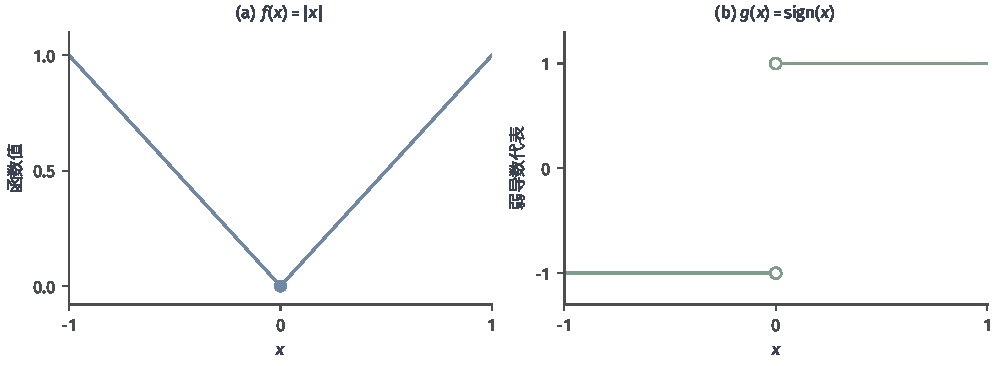
\includegraphics[width=169mm]{figures/01-mathematical-preliminaries-upper/02-linear-algebra-and-geometry/matplotlib/concepts-analysis-functional/weak-derivative.pdf}
 \functionalinlinefigurecaption{fig:functional-weak-derivative}
   {$f(x)=|x|$与其一阶弱导数$g(x)=\operatorname{sgn}(x)$。左图原点为连续尖点；右图两段分别为$-1$与$1$，空心端点表示经典导数在原点未定义。弱导数在原点的代表值可以任取，积分恒等式不受影响。}
\end{minipage}
\end{fullwidth}

\subsection{Sobolev空间}
\label{subsec:sobolev-spaces}

普通弱导存在还没有控制函数及导数的整体大小。本小节把规定阶弱导与原函数一起纳入范数，先确定成员与微分的定义域，再证明极限中的导数仍属于同一个函数；$p=2$的内积结构与$p=\infty$的补充范围分别标明。

\subsubsection{函数与弱导的共同积分控制}
\label{subsubsec:sobolev-members-norm}

\paragraph{$W^{k,p}$的成员与范数}

固定开域$\Omega\subset\mathbb R^d$、整数$k\ge0$及$1\le p<\infty$。为了同时控制函数偏差与规定阶的变化量，定义$W^{k,p}(\Omega)$由这样的$u$构成：
\[
  u\in L^p(\Omega),\qquad D^\alpha u\in L^p(\Omega)\quad(|\alpha|\le k),
\]
其中$D^0u=u$。局部可积性由$L^p$在紧集上的Hölder控制取得，因此这些弱导恒等式都有意义。

在这些等价类上定义
\begin{equation}
  \|u\|_{W^{k,p}}
  =\left(\sum_{|\alpha|\le k}\|D^\alpha u\|_p^p\right)^{1/p}.
  \label{eq:functional-sobolev-norm}
\end{equation}
零阶项控制函数本身，其余项控制各规定阶的变化量。有限个$L^p$分量的线性、正定与Minkowski不等式保证这是一个范数；只累计某一阶导数通常无法区分常数等零方向，不能不另作处理就替代当前全范数。

在有限区间$(-1,1)$上回用绝对值的弱导计算：函数和符号函数都属于每个有限$p$的$L^p$，故$|x|\in W^{1,p}(-1,1)$。阶跃虽属于该区间的$L^p$，但它的一阶分布导数是Dirac、没有普通局部可积表示，因此不属于$W^{1,p}$。这里用成员判定承接前例，不重复分部积分过程。

\paragraph{弱微分的定义域与误差控制}

对$|\alpha|\le k$，把弱微分看成映射
\[
  D^\alpha:W^{k,p}(\Omega)\to L^p(\Omega),
\]
由范数中包含该项直接得到
\[
  \|D^\alpha u\|_p\le\|u\|_{W^{k,p}}.
\]
相减后同样得到$\|D^\alpha(u-v)\|_p\le\|u-v\|_{W^{k,p}}$，因此这是在指定输入范数和定义域下的有界线性操作。

但这项控制不能被改写成“微分在任意$L^p\to L^p$上都有界”：普通$L^p$成员未必有该阶弱导，即使有导数，也没有这里的共同范数控制。输出仍是体内的弱导等价类，域内点值与整条边界记录要由后面的点值与边界读取按其输出类型另建条件。

\subsubsection{Sobolev空间的完备性}
\label{subsubsec:sobolev-completeness}

\paragraph{分量极限与弱导恒等式}

取$W^{k,p}$柯西列$(u_n)$。因为每一分量范数都不超过全范数，
\[
  \|D^\alpha u_n-D^\alpha u_m\|_p\le\|u_n-u_m\|_{W^{k,p}},
\]
故$(D^\alpha u_n)$对每个$|\alpha|\le k$都是$L^p$柯西列。回用已证明的$L^p$完备性，取得各分量极限
\[
  u_n\to v_0,\qquad D^\alpha u_n\to v_\alpha.
\]
此时它们还只是一组$L^p$元素，尚未证明彼此有导数关系。

固定$\varphi\in C_c^\infty(\Omega)$，对每个$n$写
\[
  \int_\Omega D^\alpha u_n\,\varphi\,\mathrm dx
  =(-1)^{|\alpha|}\int_\Omega u_nD^\alpha\varphi\,\mathrm dx.
\]
若$1<p<\infty$，用共轭指数$q$估计两侧差积分，分别不超过
\[
\begin{aligned}
  \left|\int(D^\alpha u_n-v_\alpha)\varphi\,\mathrm dx\right|
  &\le\|D^\alpha u_n-v_\alpha\|_p\,\|\varphi\|_q,\\
  \left|\int(u_n-v_0)D^\alpha\varphi\,\mathrm dx\right|
  &\le\|u_n-v_0\|_p\,\|D^\alpha\varphi\|_q;
\end{aligned}
\]
测试光滑且紧支撑，保证$\varphi$与$D^\alpha\varphi$在有限测度支撑上有界，两个$q$范数有限，两式右端随$n\to\infty$趋零。$p=1$时则分别以测试函数及其导数的上确界乘$L^1$误差，完成同样的极限传递。于是对所有测试都有
\[
  \int_\Omega v_\alpha\varphi\,\mathrm dx
  =(-1)^{|\alpha|}\int_\Omega v_0D^\alpha\varphi\,\mathrm dx.
\]
正是弱导定义把原本独立取得的各分量重新联系为同一个$v_0$的弱导$v_\alpha=D^\alpha v_0$，而不是仅凭记号称$v_\alpha$为导数。

各$v_\alpha$都属于$L^p$，因此$v_0\in W^{k,p}$；有限个分量的$L^p$误差都趋零，再相加开$p$次根，
\[
  \|u_n-v_0\|_{W^{k,p}}^p
  =\sum_{|\alpha|\le k}\|D^\alpha u_n-v_\alpha\|_p^p\longrightarrow0,
\]
便得到$u_n\to v_0$的Sobolev范数收敛。这样对有限$1\le p<\infty$完成了Banach性质；过程中没有要求边界光滑，也没有推出逐点或边界读取。

\paragraph{$H^k$的Hilbert结构}

固定$p=2$并记$H^k(\Omega)=W^{k,2}(\Omega)$，定义
\[
  \langle u,v\rangle_{H^k}
  =\sum_{|\alpha|\le k}\int D^\alpha u\,D^\alpha v.
\]
各项积分存在、双线性和对称性由$L^2$内积继承，零阶项保证正定，诱导范数正是上面选定的$W^{k,2}$范数。前一单元已经证明该范数下完备，现在才能称$H^k$为Hilbert空间；不能只把多个内积相加，就省略“极限中导数关系”的核验。后面的正交分解与函数目标可据此使用Hilbert工具，具体点值、边界迹和零边界闭包仍在位置读取一节处理。

\subsubsection{本质上界控制的补充范围}
\label{subsubsec:sobolev-infty-supplement}

若还要允许$p=\infty$，可另定义$W^{k,\infty}(\Omega)$，要求$u$及规定阶普通弱导都属于$L^\infty$，并采用
\[
  \max_{|\alpha|\le k}\|D^\alpha u\|_\infty.
\]
这是本质最大控制的共同范数，不把$\sum\|D^\alpha u\|_p^p$直接代入无穷指数，也不把这一补充推广写成正文已经完成的结论。其完备性若展开，仍可沿用“分量极限—测试恒等式—原空间极限”的同一路线，但改用$L^\infty$完备性，并以本质上界误差乘测试函数（或其导数）的$L^1$范数传递积分。这里只标清它与有限$p$论证相同的职责和不同的估计；正文后续主要使用$H^1$，不另行扩展一般嵌入定理或迹定理。
\section{函数的线性读取与正交表示}
\label{sec:linear-readouts-orthogonal}

前面把函数空间本身作为对象，建立了$L^2$范数、弱导与Sobolev空间。本节固定一个已经选定的实Hilbert函数空间$H$，研究两类具体读取：把函数映成标量的线性读数，以及把函数分解成一组正交方向上的记录。有限维线性代数中，最近分量、坐标变换和点值都是熟悉操作；无限维时，下确界是否达到、读数是否被范数控制、记录是否完备，都必须重新逐条检验。闭子空间投影与有界线性泛函表示是后面所有系数记录和位置记录的共同工具，先一并建立。

\subsection{有界线性泛函的表示}
\label{subsec:bounded-functional-representation}

先证明闭子空间确有最近分量，再把有界标量读数表示为内积中的一个固定方向。两者是工具与其应用的关系：投影先用来研究表示，随后又被正交展开反复调用。

\subsubsection{闭子空间的正交投影}
\label{subsubsec:orthogonal-projection}

\paragraph{最近分量的存在与正交性}

固定实Hilbert空间$H$、闭线性子空间$M\subset H$及$f\in H$，记
\[
d=\inf_{u\in M}\|f-u\|.
\]
距离是下确界，事先并不保证有$u\in M$达到它。下面的定理把存在性、正交特征和唯一性一次建立起来。

\begin{theorem}[正交投影]
\label{thm:orthogonal-projection}
设$H$为实Hilbert空间，$M\subset H$为闭线性子空间，$f\in H$。则存在唯一的$p\in M$使$\|f-p\|=d$，且该$p$满足$f-p\perp M$；反之，任何$p\in M$满足$f-p\perp M$都达到这一下确界。
\end{theorem}

\begin{proof}
取极小化列$u_n\in M$使$\|f-u_n\|\to d$。对任意$n,k$，因$(u_n+u_k)/2\in M$，由定义$\|f-(u_n+u_k)/2\|\ge d$。平行四边形恒等式给出
\[
\|(f-u_n)+(f-u_k)\|^2+\|(f-u_n)-(f-u_k)\|^2
=2\|f-u_n\|^2+2\|f-u_k\|^2.
\]
左端第一项等于$4\|f-(u_n+u_k)/2\|^2\ge 4d^2$，左端第二项正是$\|u_n-u_k\|^2$，故
\[
\|u_n-u_k\|^2\le 2\|f-u_n\|^2+2\|f-u_k\|^2-4d^2\longrightarrow0.
\]
$(u_n)$因而为Cauchy列。$H$完备，$u_n\to p\in H$；$M$闭，故$p\in M$；范数连续给出$\|f-p\|=d$，存在性成立。

再证正交性。任取$h\in M$和实数$t$，$p+th\in M$，故
\[
\|f-p-th\|^2\ge d^2=\|f-p\|^2.
\]
展开左端：$\|f-p\|^2-2t\langle f-p,h\rangle+t^2\|h\|^2$。这是关于$t$的二次函数，在$t=0$处取得最小值；因$M$是线性空间，$t$可正可负，两侧导数都允许，故一次项系数必须为零：$\langle f-p,h\rangle=0$。由$h$任意，$f-p\perp M$。

最后证唯一性与反向刻画。若$p\in M$且$f-p\perp M$，则对任意$u\in M$，$p-u\in M$，于是
\[
\|f-u\|^2=\|f-p\|^2+\|p-u\|^2\ge\|f-p\|^2,
\]
等号当且仅当$u=p$。既达到下确界的$p$唯一，又满足正交性；已证存在的$p$也满足同一分解，两个角色由同一元素担任。
\end{proof}

记$p=P_Mf$，称为$f$在$M$上的\term{正交投影}。由唯一分解$f=P_Mf+(f-P_Mf)$，其中$P_Mf\in M$而$f-P_Mf\in M^\perp$，可得$P_M$线性：对$af+bg$，$aP_Mf+bP_Mg\in M$，其余量$a(f-P_Mf)+b(g-P_Mg)\in M^\perp$，由分解唯一即等于$P_M(af+bg)$。又
\begin{equation}
\label{eq:functional-projection-error-decomposition}
\|f\|^2=\|P_Mf\|^2+\|f-P_Mf\|^2,
\end{equation}
故$\|P_Mf\|\le\|f\|$；投影作为线性算子的误差传播统一放在算子框架中讨论。

\paragraph{闭性与完备性各自保障哪一步}

上面证明的两步桥梁不能省去：极小化列成为Cauchy列靠平行四边形恒等式，极限留在$M$内靠$M$闭，极限存在靠$H$完备。三者缺一会出什么问题，用一个具体例子看清楚。

在$L^2([0,1],\mathrm dx)$中取阶跃$q=\mathbb I_{(1/2,1]}$，令连续函数
\[
u_n(t)=
\begin{cases}
0,&t\le1/2,\\
n(t-1/2),&1/2<t<1/2+1/n,\\
1,&t\ge1/2+1/n.
\end{cases}
\]
$u_n$连续，且与$q$只在$(1/2,1/2+1/n)$上相差$1-n(t-1/2)$，直接积分
\[
\|u_n-q\|_2^2=\int_{1/2}^{1/2+1/n}(1-n(t-1/2))^2\,\mathrm dt=\frac1{3n}\to0.
\]
但$q$的$L^2$等价类没有任何连续代表：连续函数在一点的值决定其在一个邻域上的值，而$q$在$1/2$两侧本质不同。于是连续函数构成的集合$C([0,1])$在$L^2$中不闭：极限$q$离开了该集合。反过来，若把环境取为$C([0,1])$并配$L^2$范数，该空间又不完备：$(u_n)$在$L^2$范数下是Cauchy列，却不在$C([0,1])$中有极限。闭性保障“极限留在可行集内”，完备性保障“环境中有极限可取”，两件事不能合并成一句“无限维中自然成立”。

\begin{figure}[h]
  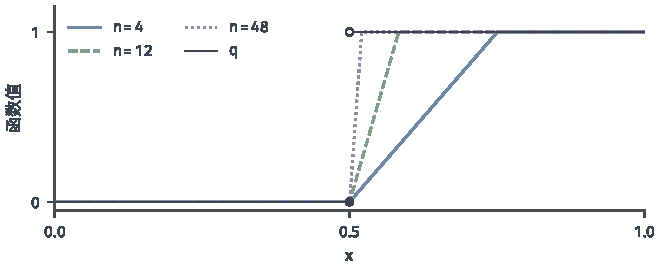
\includegraphics[width=112mm]{figures/01-mathematical-preliminaries-upper/02-linear-algebra-and-geometry/matplotlib/comprehension-additions/functional-incomplete-continuous.pdf}
  \caption{连续斜坡$u_n(t)=\operatorname{clip}(n(t-1/2),0,1)$取$n=4,12,48$（实、虚、点线），灰黑阶跃为$q=\mathbb I\{t>1/2\}$。黑实点与空心圈标明阶跃在$1/2$处的取值；斜坡逐点趋于阶跃，但$\|u_n-q\|_2^2=1/(3n)\to0$，$u_n$在一致范数下并不收敛到任何连续函数。图说明$C([0,1])$在$L^2$范数下不闭，不表示该阶跃有连续代表。}
  \label{fig:vol1-add-functional-incomplete-continuous}
\end{figure}

后面Riesz表示对闭零空间使用这条投影；正交系数对有限方向的张成使用这条投影。一般闭凸集合上的最近点涉及变分不等式，留给函数值拟合任务处理，因为那里改变的是可行集合，而非线性记录方向。

\subsubsection{有界线性泛函与Riesz表示}
\label{subsubsec:riesz-representation}

\paragraph{标量读取与有界性}

固定实Hilbert空间$H$，映射$L:H\to\mathbb R$称为\term{线性泛函}，若
\[
L(af+bg)=aL(f)+bL(g)\qquad(\forall f,g\in H,\ a,b\in\mathbb R).
\]
它把一个函数读成一个标量。若存在与$f$无关的常数$C$使
\[
|L(f)|\le C\|f\|\qquad(\forall f\in H),
\]
则称$L$有界，并定义最佳常数
\[
\|L\|=\sup_{\|f\|\le1}|L(f)|.
\]
有界性是“单位球上的输出有统一界”，与某个具体$f$的输出数值有限不是同一回事。

每个固定方向$h\in H$都给出一个有界读取$L_h(f)=\langle f,h\rangle_H$：由Cauchy–Schwarz，$|L_h(f)|\le\|h\|\|f\|$，故$\|L_h\|\le\|h\|$；取$f=h/\|h\|$（$h\ne0$）时$L_h(f)=\|h\|$，反向不等式成立，$\|L_h\|=\|h\|$。自然的反向问题是：每一个有界线性读取是否都来自某个固定方向？下面的Riesz表示给出肯定回答。

\paragraph{由零空间投影证明表示}

\begin{theorem}[Riesz表示]
\label{thm:riesz}
设$H$为实Hilbert空间，$L:H\to\mathbb R$为有界线性泛函。则存在唯一的$h_L\in H$，使
\begin{equation}
\label{eq:functional-riesz-representation}
L(f)=\langle f,h_L\rangle_H\qquad(\forall f\in H),
\end{equation}
且$\|L\|=\|h_L\|_H$。
\end{theorem}

\begin{proof}
若$L=0$，取$h_L=0$即可。下设$L\ne0$。

零空间$N=\{f\in H:L(f)=0\}$是$H$的线性子空间。它闭：若$f_n\in N$且$f_n\to f$，由有界性$|L(f)|=|L(f)-L(f_n)|\le\|L\|\|f-f_n\|\to0$，故$f\in N$。

取$v\in H$使$L(v)\ne0$。设$v=p+w$为$v$在$N$上的正交投影分解：$p=P_Nv\in N$，$w=v-p\perp N$。由$L(w)=L(v)-L(p)=L(v)\ne0$知$w\ne0$。

对任意$f\in H$，构造
\[
f-\frac{L(f)}{L(w)}\,w.
\]
它在$L$下的像为$L(f)-\frac{L(f)}{L(w)}L(w)=0$，故属于$N$；而$w\perp N$，与$w$取内积得零：
\[
\langle f,w\rangle-\frac{L(f)}{L(w)}\|w\|^2=0,
\qquad\text{即}\qquad
\langle f,w\rangle=\frac{L(f)}{L(w)}\|w\|^2.
\]
令
\begin{equation}
\label{eq:functional-riesz-direction}
h_L=\frac{L(w)}{\|w\|^2}\,w,
\end{equation}
则$L(f)=\langle f,w\rangle\,L(w)/\|w\|^2=\langle f,h_L\rangle$，表示成立。

唯一性：若$h,h'$都满足$L(f)=\langle f,h\rangle=\langle f,h'\rangle$，则$\langle f,h-h'\rangle=0$对一切$f$成立；取$f=h-h'$得$\|h-h'\|^2=0$。

范数等式：由$|L(f)|\le\|h_L\|\|f\|$得$\|L\|\le\|h_L\|$。反向，$L(h_L)=\langle h_L,h_L\rangle=\|h_L\|^2$，故$\|h_L\|=|L(h_L)|/\|h_L\|\le\|L\|$。两端相等。
\end{proof}

表示结论只适用于已经有界的标量泛函。它不能事先证明任意点读数有界——那要在点值一节单独检验；也不能把输出为整条边界函数的迹算子缩成单个内积方向，因为迹的输出不是标量。有界性、标量输出、Hilbert内积三者齐备，Riesz才给出一个方向。

\subsection{正交展开与系数记录}
\label{subsec:orthogonal-expansions-coefficients}

本小节固定表示方向，研究已知函数如何按正交方向分解、截断后丢失多少，以及不同有限记录之间如何转换。三个子题按同一记录任务的组成分工：建立方向记录、评估有限保留、转换记录坐标。

\subsubsection{正交系数与函数展开}
\label{subsubsec:orthogonal-records}

\paragraph{正交方向与完整记录}

设$H$为实Hilbert空间，序列$(e_j)_{j\ge1}\subset H$满足
\[
\langle e_j,e_k\rangle_H=\delta_{jk}.
\]
称$(e_j)$为正交归一序列；若所有有限线性组合在$H$中稠密，即$\overline{\operatorname{span}}\{e_j\}=H$，则称它为$H$的\term{完备正交系}（也叫正交归一基）。环境空间完备不等于所选正交系覆盖全部方向：在$\ell^2$中取仅偶数坐标非零的方向$e_2,e_4,\dots$，它们正交归一，其闭张成是$\ell^2$的真闭子空间，奇数方向整个缺失。

对前$m$个方向的张成$S_m=\operatorname{span}\{e_1,\dots,e_m\}$使用正交投影定理。$S_m$有限维因而闭。记$c_j=\langle f,e_j\rangle$，则
\begin{equation}
\label{eq:functional-orthogonal-partial-projection}
P_{S_m}f=\sum_{j=1}^m c_j e_j.
\end{equation}
验证：右端属于$S_m$，且对每个$k\le m$，$f-\sum_{j\le m}c_je_j$与$e_k$的内积为$c_k-c_k=0$，故与整个$S_m$正交。每个系数$c_j$正是前一小节$h_L=e_j$时的有界标量读取，$|c_j|\le\|f\|$。

正交性给出逐项相消的误差：
\begin{equation}
\label{eq:functional-bessel}
\|f-P_{S_m}f\|^2=\|f\|^2-\sum_{j=1}^m|c_j|^2,
\end{equation}
因而Bessel不等式$\sum_{j=1}^m|c_j|^2\le\|f\|^2$对一切$m$成立，正项级数$\sum_j|c_j|^2$收敛且不超过$\|f\|^2$。

\begin{theorem}[完备正交系与Parseval等式]
\label{thm:parseval}
设$(e_j)$为$H$的完备正交系，$c_j=\langle f,e_j\rangle$。则
\[
\begin{aligned}
\lim_{m\to\infty}\|f-\sum_{j=1}^m c_je_j\|=0,
\qquad
\|f\|^2=\sum_{j=1}^\infty|c_j|^2,\\
f=\sum_{j=1}^\infty c_je_j\quad(\text{依}H\text{范数}).
\end{aligned}
\]
\end{theorem}

\begin{proof}
记$s_m=\sum_{j\le m}c_je_j=P_{S_m}f$。由$S_m$张成在$H$中稠密，对$\varepsilon>0$存在有限组合$u=\sum_{j\le m_0}a_je_j$使$\|f-u\|<\varepsilon$。$s_{m_0}$是$f$在$S_{m_0}$上的最佳逼近，故$\|f-s_{m_0}\|\le\|f-u\|<\varepsilon$；而由Bessel误差公式，$\|f-s_m\|^2$随$m$增大单调不增（尾余项为正项级数尾和），故对一切$m\ge m_0$，$\|f-s_m\|<\varepsilon$。范数展开与Parseval等式随之成立。
\end{proof}

若正交系不完备，$P_{S_m}f$只收敛到$f$在其闭张成上的投影，正交余部$\overline{\operatorname{span}}\{e_j\}^\perp$中的分量永远保留。Bessel不等式与Parseval等式的差别正是覆盖条件的差别，不能混用。

\paragraph{傅里叶方向的计算与遗漏}

在$L^2([-\pi,\pi],\mathrm dx)$中取\term{傅里叶基}，即
\[
e_0=\frac1{\sqrt{2\pi}},\qquad
e_j^c=\frac{\cos(jx)}{\sqrt\pi},\qquad
e_j^s=\frac{\sin(jx)}{\sqrt\pi}\quad(j\ge1).
\]
直接积分给出
\[
\begin{aligned}
\int_{-\pi}^{\pi}\cos(jx)\cos(kx)\,\mathrm dx=\pi\delta_{jk},
\qquad
\int_{-\pi}^{\pi}\sin(jx)\sin(kx)\,\mathrm dx=\pi\delta_{jk},\\
\int_{-\pi}^{\pi}\cos(jx)\sin(kx)\,\mathrm dx=0.
\end{aligned}
\]
它们构成正交归一系；经典三角级数理论给出其完备性。正交评估的是函数内积：例如$1$与$x$的乘积在正负半区间相消，不等于“平面图像互相垂直”这种几何画面。

取$f(x)=x$。$f$是奇函数，故常数项与全部余弦系数为零。对第一个正弦方向分部积分：
\[
\begin{aligned}
\int_{-\pi}^{\pi}x\sin x\,\mathrm dx
&=\bigl[-x\cos x\bigr]_{-\pi}^{\pi}+\int_{-\pi}^{\pi}\cos x\,\mathrm dx\\
&=-\pi(-1)+\pi(-1)\cdot(-1)+0=2\pi,
\end{aligned}
\]
故第一个正弦系数为
\[
\frac1{\sqrt\pi}\int_{-\pi}^{\pi}x\sin x\,\mathrm dx=2\sqrt\pi.
\]
一般地，$\frac1{\sqrt\pi}\int_{-\pi}^{\pi}x\sin(jx)\,\mathrm dx=2\sqrt\pi\,(-1)^{j+1}/j$。Parseval等式此时成为可复算的检验：
\[
\sum_{j=1}^\infty\frac{4\pi}{j^2}=\frac{2\pi^3}{3}=\int_{-\pi}^{\pi}x^2\,\mathrm dx,
\]
其中$\sum_j1/j^2=\pi^2/6$。

保留常数及前$m$组正弦、余弦即得傅里叶截断。只取余弦方向时投影恒为零，增加再多同类方向也不能逼近$x$——方向选错时数量不补覆盖。完整三角系在上述$L^2$范数下完备，但范数收敛不自动承诺逐点收敛或一致收敛；截断误差在下一小节专门计算。

\subsubsection{正交截断与尾误差}
\label{subsubsec:truncation-tail}

固定同一$f$与同一完备正交系，只改变保留项数$m$，$s_m=\sum_{j\le m}c_je_j$是一个函数序列。由上节误差公式，
\begin{equation}
\label{eq:functional-truncation-tail}
\|f-s_m\|^2=\sum_{j>m}|c_j|^2\longrightarrow0,
\end{equation}
收敛来自可求和级数$\sum_j|c_j|^2$的尾部消失。每个$s_m$在当前前$m$个方向内最佳，但这并未与所有同规模非线性表示作比较——表示方向怎样选择由有限表示任务处理，这里固定方向后只回答截断是否收敛。

式\eqref{eq:functional-truncation-tail}只控制所选空间范数。点值误差要等点值读取建立相应有界常数后才能传递；一致误差还要求对所有位置有统一的读取界。不能从$L^2$尾项直接跳到逐点或一致收敛。另外，积分谱中的$L^2$归一方向与核RKHS中的归一方向尺度不同，相应的两种尾误差在Mercer展开处分别给出，此处不提前引入尚未定义的权重。

\subsubsection{系数与有限读数的转换}
\label{subsubsec:record-conversion}

\paragraph{换基与记录矩阵}

先限定$f=\sum_{j=1}^m a_j\varphi_j$属于已知有限维张成。线性无关的方向使系数由函数唯一确定；方向相关时，不同系数组可表示同一函数；一般非线性参数族则不能套用线性基的结论。

对$f(t)=a+bt$，把基$(1,t)$改为$(1,t-c)$，逐项展开
\[
f(t)=a+bt=(a+bc)+b(t-c),
\]
新系数为$(a+bc,b)$。这只改变记录坐标，目标函数及其取值完全相同。改读$f(0),f(1)$时，
\[
\begin{pmatrix}f(0)\\f(1)\end{pmatrix}
=\begin{pmatrix}1&0\\1&1\end{pmatrix}\begin{pmatrix}a\\b\end{pmatrix},
\]
由$f(0)=a$、$f(1)-f(0)=b$恢复系数。若只读$f(0)$，斜率方向不可见：可逆矩阵与缺失列分别意味着记录完整与方向丢失。

对一般线性读数$L_i$（$i=1,\dots,n$），记录矩阵$A\in\mathbb R^{n\times m}$的第$(i,j)$项为
\[
A_{ij}=L_i(\varphi_j).
\]
点值读数给出$A_{ij}=\varphi_j(x_i)$，积分读数给出$A_{ij}=\int\varphi_j w_i\,\mathrm d\mu$。代入前须核对定义域、积分存在与输出类型，再执行矩阵换算$L(f)=Aa$。

\paragraph{有限表示之外的边界}

矩阵可逆只说明：在指定的有限维候选张成内部，记录与系数的转换唯一。若候选扩大到任意函数，同样$n$条读数可能对应无穷多个函数——这是新增的单射性问题，交给有限读数的可识别性任务，不在已知表示的换算中提前宣告恢复成功。无限表示还须指定收敛范数、尾误差和极限归属；上面的正交截断提供了一种可核验情形，其他表示按各自条件判断，不能把有限求和矩阵原样当成无限展开的计算保证。

\subsection{点值与边界读取}
\label{subsubsec:point-boundary-readouts}

本小节按输出位置区分单点取值与整条边界记录。前者输出标量，后者通常输出边界函数等价类。共同要求是：先明确输入元素和合法代表，再判断读取是否存在并受范数控制。

\subsubsection{域内点值读取}
\label{subsubsec:point-evaluation}

\paragraph{等价类与合法代表}

在通常Lebesgue测度的$[0,1]$上，零函数与仅在$x=1/2$取$1$的函数是同一个$L^2$元素，却给出不同的点值。因此任取一个可测代表再读取该点，不能在商空间上定义同一个数：点值读取首先不是“是否有界”，而是“在等价类上是否良定义”。

该反例依赖单点的可测性与零测度。若$\mu(\{x\})>0$，两个几乎处处相等的代表在$x$处必相等，且有限$p$时
\[
|f(x)|\le\mu(\{x\})^{-1/p}\|f\|_p,
\]
正质量单点要另作判断，不能把零测点的结论推广到所有测度。

若某等价类存在连续代表，且测度在定义域上全支撑，则这样的代表唯一：两个连续代表若在一点不同，差异会延伸到一个正测度邻域，与几乎处处相等矛盾。这里解决的是唯一性；代表是否存在仍需额外正则性结论。若输入本来就是真实连续函数，或已由条件选出唯一连续代表，点读数有确定含义，但这个数是否被当前范数控制仍未解决。

\paragraph{点值的有界性与维数条件}

对已经良定义的线性点读数$L_x(f)=f(x)$，提出有界性要求
\[
|L_x(f)|\le C_x\|f\|,
\]
其中$C_x$可依赖位置$x$，但不能依赖$f$。在$[0,1]$上取连续尖峰
\[
f_n(t)=\max(1-nt,0),
\]
直接算得$\|f_n\|_2^2=\int_0^{1/n}(1-nt)^2\mathrm dt=1/(3n)$，而$f_n(0)=1$，比值$\sqrt{3n}$无界。故连续函数上的$L^2$范数不能控制原点读取；零点是闭区间中允许的输入位置，此例不替代一般区域的边界迹定理。

与积分读取对照：$L_w(f)=\int fw\,\mathrm d\mu$在$w\in L^2$时由Cauchy–Schwarz给出$|L_w(f)|\le\|w\|_2\|f\|_2$；正交系数也是这类内积读取。问题出在点读数与所选范数的组合，而非线性读取本身。

在一维有界区间$I=(a,b)$上，Sobolev范数确实控制点值，下面把这件事完整做完。设$u\in H^1(I)$，弱导$g\in L^2(I)$。令
\[
F(x)=\int_a^x g(t)\,\mathrm dt.
\]
积分基本定理给出$F$绝对连续；分部积分核对其弱导为$g$，故$u-F$的分布导数为零。要得到$u$的点值，还须说明零分布导数迫使$u-F$为常数。

设$T_{u-F}$为$u-F$诱导的分布。先取积分为零的紧支撑光滑测试$\psi$：其积分原函数$\varphi(x)=\int_a^x\psi$仍紧支撑且$\varphi'=\psi$，由$u-F$分布导数为零得
\[
0=\int(u-F)\varphi'=\int(u-F)\psi.
\]
固定一个积分为$1$的测试$\rho$。任意测试$\psi$可分解为$(\int\psi)\rho+\bigl(\psi-(\int\psi)\rho\bigr)$，第二项积分为零，被上式灭掉；于是
\[
T_{u-F}(\psi)=c\int\psi,\qquad c=T_{u-F}(\rho).
\]
即分布$T_{u-F}$等于常数$c$作为普通函数的分布。由普通函数表示分布的唯一性，$u-F=c$几乎处处。于是$c+F$是$u$的绝对连续代表，其每一点值合法且唯一。

记区间长度$L=b-a$。由平方积分平均，存在$y\in I$使
\[
|u(y)|\le L^{-1/2}\|u\|_2.
\]
对闭区间中任意$x$，$u(x)-u(y)=\int_y^x g$，再用Cauchy–Schwarz，
\begin{equation}
\label{eq:functional-point-evaluation-embed}
|u(x)|\le L^{-1/2}\|u\|_2+L^{1/2}\|g\|_2.
\end{equation}
该估计对闭区间中的$x$统一成立：一维$H^1$既解决单点有界，也给出全域控制。

一维结论不能跨维照搬。在三维域内部固定$x_0$，取光滑紧支撑$\varphi$且$\varphi(0)=1$，令$f_n(x)=\varphi(n(x-x_0))$，$n$足够大时支撑在域内。换元给出
\[
\|f_n\|_2^2=n^{-3}\|\varphi\|_2^2,\qquad
\|\nabla f_n\|_2^2=n^{-1}\|\nabla\varphi\|_2^2,\qquad
f_n(x_0)=1.
\]
于是$f_n(x_0)/\|f_n\|_{H^1}\asymp n^{1/2}\to\infty$：即使限制光滑函数，三维$H^1$范数也不能控制该点读数。一般逐点常数$C_x$可随位置增长，只有$\sup_xC_x<\infty$才给统一控制。取整条实轴上由$f(t)=bt$组成、范数为$|b|$的函数空间，点读数常数恰为$|x|$；真正把输入域限制为$[-3,3]$，才能取得统一常数$3$——图\ref{fig:vol1-add-functional-pointwise-bound-growth}同时画出两条单位范数函数与逐点常数，注意显示窗口不是定义域，$C_x$在实轴上无界。

\begin{figure}[h]
  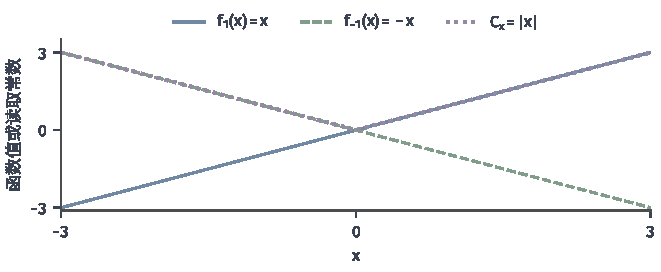
\includegraphics[width=112mm]{figures/01-mathematical-preliminaries-upper/02-linear-algebra-and-geometry/matplotlib/comprehension-additions/functional-pointwise-bound-growth.pdf}
  \caption{在$H=\{f(t)=bt\}$、$\|f\|_H=|b|$的空间中，单位范数函数$f_1(t)=t$与$f_{-1}(t)=-t$（实、虚线），点$x$处的最佳读取常数$C_x=|x|$（点线）。$x$离原点越远，同样范数函数在该点的值越大；在整条实轴上$C_x$无界，统一读取界不存在。显示窗口$[-3,3]$不是输入域。}
  \label{fig:vol1-add-functional-pointwise-bound-growth}
\end{figure}

\paragraph{再生核Hilbert空间与正向表示}

在真实函数组成的实Hilbert空间$H$中，把每个点读数$L_x:f\mapsto f(x)$都有界作为空间条件，称这样的空间为\term{再生核Hilbert空间}（RKHS）。先有点读数有界，才能调用Riesz表示取得唯一$K_x\in H$使
\begin{equation}
\label{eq:functional-reproducing-property}
f(x)=\langle f,K_x\rangle_H\qquad(\forall f\in H).
\end{equation}
定义$K(x,z)=K_z(x)=\langle K_z,K_x\rangle_H$，称它为$H$的\term{再生核}。由内积对称性，$K(x,z)=K(z,x)$；对任意有限点组与系数，
\[
0\le\Big\|\sum_i a_iK_{x_i}\Big\|_H^2
=\sum_{i,j}a_ia_jK(x_i,x_j),
\]
故核对称且Gram矩阵半正定；满足这条Gram半正定性的$K$称为\term{正定核}。$K:X\times X\to\mathbb R$是标量核。

由Riesz最佳常数，
\begin{equation}
\label{eq:functional-rkhs-pointwise-bound}
\|L_x\|=\|K_x\|_H=\sqrt{K(x,x)}.
\end{equation}
核对角上界$K(x,x)\le M^2$才使同一个$M$控制所有点：这解释了何种空间结构支持统一读取。

固定仿射核$K(x,z)=1+xz$，令
\[
H=\{f(t)=a+bt\},\qquad
\langle a+bt,a'+b't\rangle_H=aa'+bb'.
\]
取$K_x(t)=1+xt$，逐项核对：
\[
\langle a+bt,K_x\rangle_H=a\cdot1+b\cdot x=a+bx=f(x),
\]
$\|f\|_H^2=a^2+b^2$，$\|K_x\|_H^2=1+x^2$。抽象的再生关系在这里有完整坐标计算。

\paragraph{由半正定核反向构造空间}

正向构造从空间出发得到核；反过来，固定非空集合$X$与实对称半正定核$K$，也能唯一造出以$K$为再生核的RKHS。

先用有限核截面的形式线性组合建立双线性型
\[
\Big\langle\sum_i a_iK_{x_i},\sum_jb_jK_{z_j}\Big\rangle
=\sum_{i,j}a_ib_jK(x_i,z_j).
\]
Gram二次型半正定只给出半内积：存在非零组合长度为零。半内积的Cauchy–Schwarz$|\langle f,g\rangle|\le\|f\|\|g\|$表明，零长度方向在每点读数均为零，并有
\[
|f(x)|=|\langle f,K_x\rangle|\le\sqrt{K(x,x)}\,\|f\|.
\]
因此先商去零长度方向，读取在商空间上良定义，不能直接声称半内积空间已是Hilbert空间。

对该内积空间作完备化。逐点读取界使每条Cauchy列在每个$x$处取得确定极限（$|f_n(x)-f_m(x)|\le\sqrt{K(x,x)}\|f_n-f_m\|$），并使等价Cauchy列定义同一函数。若完成后的元素在所有点为零，它与每个$K_x$正交；核截面张成稠密，故该元素为零——完备化到函数空间的表示因此单射。核截面内积与再生关系在极限下保留，得到以$K$为再生核的RKHS。任何其他同核RKHS在核截面张成上内积相同，由稠密性唯一延拓，故空间由核唯一确定。半正定允许有限Gram矩阵奇异，不能把“正定核”的常用约定误读为所有Gram矩阵严格正定。

这条构造只需集合与半正定核，不需事先给测度。后面的积分谱还要另给测度及连续性、紧性条件；RKHS是具有稳定点读数的Hilbert函数空间，不是与Hilbert空间或Banach空间互斥的类别。

\paragraph{固定点的函数误差与位置误差}

先固定$x$和核空间，仅把$f$改为$f+h$。由再生关系，
\begin{equation}
\label{eq:functional-rkhs-error-fixedpoint}
|(f+h)(x)-f(x)|=|\langle h,K_x\rangle_H|
\le\sqrt{K(x,x)}\,\|h\|_H.
\end{equation}
这是有界读取在固定点的应用。再固定同一$f$，只把位置$x$改为$z$：
\[
f(x)-f(z)=\langle f,K_x-K_z\rangle_H,
\]
故
\[
\begin{aligned}
|f(x)-f(z)|\le\|f\|_H\|K_x-K_z\|_H,\\
\|K_x-K_z\|_H^2=K(x,x)+K(z,z)-2K(x,z).
\end{aligned}
\]
位置稳定取决于核截面在空间范数中的接近。若$X$有拓扑且$K$连续，上式给出核截面随位置连续，进而给出每个$f\in H$的连续性；若还要对一整类函数统一控制，则固定该类的范数半径。单点读取有界本身未包含位置连续性，两种扰动不能混成一项。

\subsubsection{边界迹与零边界空间}
\label{subsubsec:trace-zero-boundary}

弱导空间首先由体内几乎处处等价类组成；边界条件需要一条由体内元素到边界记录的合法映射，不能任取代表后逐点限制。

\paragraph{迹的输出与连续延拓}

固定有界Lipschitz区域$\Omega\subset\mathbb R^d$、边界表面测度$\mathrm dS$与输入空间$H^1(\Omega)$。所需输出是$L^2(\partial\Omega,\mathrm dS)$中的边界函数等价类，不是某个边界点上的标量，因而不是一个Riesz方向可以表示的对象。

在光滑函数上，限制$u\mapsto u|_{\partial\Omega}$就是熟悉的边界取值。把它延拓到整个$H^1(\Omega)$需要一个前提估计。标准迹定理指出：对上述Lipschitz区域，存在常数$C_\Omega$使
\begin{equation}
\label{eq:functional-trace-inequality}
\|u|_{\partial\Omega}\|_{L^2(\partial\Omega,\mathrm dS)}
\le C_\Omega\|u\|_{H^1(\Omega)}
\qquad(\forall u\in C^\infty(\overline\Omega)).
\end{equation}
其证明通过边界局部平直化，把问题化到半空间的一维论证（与本节端点估计同源），再用光滑逼近完成；一维区间上的端点估计式\eqref{eq:functional-point-evaluation-embed}是它最简单的特例，不能冒充一般区域的证明。

对任意$u\in H^1(\Omega)$，取光滑逼近列$u_n\in C^\infty(\overline\Omega)$在$H^1(\Omega)$中收敛于$u$。由式\eqref{eq:functional-trace-inequality}，
\[
\|u_n|_{\partial\Omega}-u_m|_{\partial\Omega}\|_{L^2(\partial\Omega)}
\le C_\Omega\|u_n-u_m\|_{H^1(\Omega)},
\]
故边界限制列在$L^2(\partial\Omega)$中为Cauchy列。$L^2$完备，取得极限；若另取逼近列$v_n\to u$，混合列$(u_1,v_1,u_2,v_2,\dots)$同样$H^1$收敛，其边界列极限唯一，故极限与逼近列选择无关。以此定义连续延拓
\[
\operatorname{Tr}:H^1(\Omega)\to L^2(\partial\Omega,\mathrm dS),
\]
并保留同一范数界$\|\operatorname{Tr}u\|_{L^2(\partial\Omega)}\le C_\Omega\|u\|_{H^1(\Omega)}$。迹算子是有界线性算子，其输出类型为边界函数等价类。

\paragraph{零迹与固定边界的可行集合}

用$H^1$范数闭包定义
\[
H_0^1(\Omega)=\overline{C_c^\infty(\Omega)}^{\,H^1(\Omega)},
\]
该定义不依赖任意代表的逐点边界值。由$\operatorname{Tr}$连续且$C_c^\infty(\Omega)$中函数在边界附近为零，$H_0^1\subseteq\ker\operatorname{Tr}$。标准零迹刻画定理给出反向包含：在上述Lipschitz区域条件下，$\ker\operatorname{Tr}$恰为$C_c^\infty(\Omega)$的$H^1$闭包，故
\[
H_0^1(\Omega)=\ker\operatorname{Tr}.
\]

迹的像不能直接当成全部$L^2$边界函数。若已知合法边界数据$g=\operatorname{Tr}G$，候选集合可写成$G+H_0^1(\Omega)$：允许扰动具有零迹。这为后面的梯度拟合提供不依赖点值代表的边界接口。自由边界则允许相应边界扰动；具体自然通量由变分任务及额外正则性推导，此处不提前给所有弱解定义普通法向导数。

\section{线性算子与积分方程}
\label{sec:linear-operators-integral-equations}

本节研究函数空间之间的线性运算及其方程：先建立各类运算共用的定义域、范数与算子性质，再对积分算子检查作用是否合法、怎样改变方向，最后求解该积分运算进入的方程。共用准备与两个主体任务分别标明，不能把一般算子性质藏在积分核的例子里，也不能把求解方程与已知函数的正向积分混成同一种输出。

\subsection{线性算子的共同框架}
\label{subsec:operator-framework}

本小节只建立后面确实使用的输入输出、误差范数、伴随与紧性语言。点读数和投影是已经见过的实例，微分与迹说明定义域和目标空间也可能改变。

\subsubsection{定义域、有界性与输入误差}
\label{subsubsec:operator-domain-boundedness}

\paragraph{线性算子及所用范数}

固定赋范空间$V,W$，映射$A:V\to W$称为线性算子，若
\[
A(af+bg)=aAf+bAg.
\]
若实际只允许定义域$D(A)\subset V$中的输入，应在一开始写清该线性定义域；函数、导数或积分存在的成员条件不能省略成一个形式公式。有界算子框架先取$A$在整个$V$上定义；若只取受限定义域，须另写其所赋范数，不自动调用全空间结论。

定义算子范数
\[
\|A\|_{\mathrm{op}}=\sup_{\|f\|_V\le1}\|Af\|_W.
\]
其有限等价于存在统一常数$C$使$\|Af\|_W\le C\|f\|_V$，最佳常数就是$\|A\|_{\mathrm{op}}$。这里的有界是单位球输出有统一界，与某个输入的输出数值有限不同；对线性算子，这一条件也等价于连续性。

用同一求导公式比较定义域和范数：$D:H^1(I)\to L^2(I)$在Sobolev范数下有界，因为$\|u'\|_2\le\|u\|_{H^1}$。仅用$L^2$输入范数时，在$I=(0,2\pi)$取$f_n(x)=\sin(nx)$，则
\[
\|f_n\|_2=\sqrt\pi,\qquad \|f_n'\|_2=n\sqrt\pi,
\]
比值$n$无界，不存在统一的导数控制常数。因此不能不核对空间，就给微分运算套用后面有界紧算子的结论。

\paragraph{固定算子的输入误差传播}

固定$A$及两空间范数，输入由$f$变为$f+h$。线性先把输出差化为$Ah$，再由算子范数，
\begin{equation}
\label{eq:functional-operator-error-propagation}
\|A(f+h)-Af\|_W=\|Ah\|_W\le\|A\|_{\mathrm{op}}\|h\|_V.
\end{equation}
没有线性时，不能从“输出有界”直接写出这一差分界。正交系数、固定点值、边界迹和后面的积分算子分别在自己的输入输出范数下代入常数；位置变化由核截面差处理，数据变化后重新优化则是解映射稳定性，二者均不是这条固定算子界自动包办的结论。

\subsubsection{伴随、自伴、正与紧}
\label{subsubsec:adjoint-selfadjoint-compact}

\paragraph{伴随与二次型}

在实Hilbert空间$V,W$中固定有界线性$A:V\to W$。对每个$w\in W$，映射$f\mapsto\langle Af,w\rangle_W$是$V$上的有界标量泛函：
\[
|\langle Af,w\rangle_W|\le\|Af\|_W\|w\|_W\le\|A\|_{\mathrm{op}}\|f\|_V\|w\|_W.
\]
由Riesz表示，存在唯一$A^*w\in V$使
\[
\langle Af,w\rangle_W=\langle f,A^*w\rangle_V.
\]
$A^*$的线性：对$w_1,w_2$，$\langle f,A^*(w_1+w_2)\rangle=\langle Af,w_1+w_2\rangle=\langle f,A^*w_1+A^*w_2\rangle$对一切$f$成立，故$A^*(w_1+w_2)=A^*w_1+A^*w_2$；齐次性同理。由$|\langle Af,w\rangle|\le\|A\|\|f\|\|w\|$取得$\|A^*w\|\le\|A\|\|w\|$，故$A^*$有界且$\|A^*\|\le\|A\|$。反过来，
\[
\|Af\|_W=\sup_{\|w\|\le1}|\langle Af,w\rangle_W|
=\sup_{\|w\|\le1}|\langle f,A^*w\rangle_V|
\le\|A^*\|\|f\|_V,
\]
故$\|A\|\le\|A^*\|$，两端相等$\|A^*\|=\|A\|$。

仅当输入输出为同一Hilbert空间时定义自伴$A=A^*$。本节的正算子约定为自伴且$\langle Af,f\rangle\ge0$：自伴允许负二次型，正性另加非负要求，二者不能只凭核对称一并得到。

\paragraph{紧性及其与有界性的区别}

线性算子$A:V\to W$称为紧算子，若它把$V$中有界集合映为$W$中相对紧集合；等价地，每个有界输入列$(f_n)$的输出列$(Af_n)$有范数收敛子列。有限秩有界算子的输出落在有限维空间的有界集中，故紧。

在无限维Hilbert空间用正交归一序列检验恒等算子$I$：各$\|e_n\|=1$，$\|e_n-e_m\|=\sqrt2\ (n\ne m)$，输出列没有收敛子列，故$I$不紧。$I$有界、自伴且正，却不紧——前三种条件不替代紧性。

紧算子的算子范数极限仍紧，这是后面核逼近的桥梁。设$A_n\to A$（$\|A_n-A\|\to0$），$A_n$紧。对单位球输出$A(B)$：取$n$使$\|A_n-A\|<\varepsilon$，$A_n(B)$相对紧故有有限$\varepsilon$-网$\{y_i\}$。任取$Af$，选$y_i$使$\|A_nf-y_i\|<\varepsilon$，则
\[
\|Af-y_i\|\le\|(A-A_n)f\|+\|A_nf-y_i\|<\varepsilon+\varepsilon=2\varepsilon,
\]
故$\{y_i\}$是$A(B)$的$2\varepsilon$-网。$W$完备使闭包紧，故$A(B)$相对紧。

\subsubsection{群平均与不变方向}
\label{subsubsec:group-average}

这项沿用已建立的投影和有界算子语言，给出已知函数运算如何主动消去方向的实例。

\paragraph{群平均与不可见方向}

固定有限群$G$在函数定义域上的作用，定义
\[
Pf(x)=\frac1{|G|}\sum_{g\in G}f(gx).
\]
若放在$L^2(\mu)$中，还要求作用可测且保测度，使输入等价类上的复合与范数控制合法。群乘法是双射重排求和，故
\[
P f(hx)=\frac1{|G|}\sum_g f(ghx)=\frac1{|G|}\sum_{g'}f(g'x)=Pf(x),
\]
输出不变。重复平均给出$P^2=P$。再证自伴：对任意$h\in L^2(\mu)$，作变量替换$y=gx$并用保测度与取逆重排，
\[
\begin{aligned}
\langle Pf,h\rangle
&=\frac1{|G|}\sum_{g\in G}\int f(gx)h(x)\,\mathrm d\mu(x)\\
&=\frac1{|G|}\sum_{g\in G}\int f(y)h(g^{-1}y)\,\mathrm d\mu(y)\\
&=\int f(y)\Bigl(\frac1{|G|}\sum_{g'\in G}h(g'y)\Bigr)\,\mathrm d\mu(y)\\
&=\langle f,Ph\rangle.
\end{aligned}
\]
$P$幂等且自伴，故它是到不变函数闭子空间的正交投影。

在对称区间及对称测度上取$G=\{I,-I\}$，得$Pf(x)=[f(x)+f(-x)]/2$：偶方向保留、奇方向消去，特别是$f(x)=x$输出零。同样在中心对称的二维区域上，横坐标$f(x_1,x_2)=x_1$也被平均为零。被主动移除的信息可能正是任务需要的方向，故这种不变性不单独给出预测或泛化保证。

\subsection{积分算子的作用与方向}
\label{subsubsec:integral-operator-directions}

固定标量核和测度后，积分算子把已知函数送成另一个函数（积分结果函数）。点值核表示可在附加条件下提供同一核，但一般可积核允许正负：它既不必正定，也不是输出非负测度的测度核。

\subsubsection{平方可积核的有界性与紧性}
\label{subsubsec:hilbert-schmidt}

\paragraph{从核截面取得整函数输出}

这里讨论的是由各位置的积分值组成的整个输出函数，不涉及复分析中的整函数概念。
固定$\sigma$有限测度空间$(X,\mu)$、$(Y,\nu)$以及
\[
K\in L^2(Y\times X,\nu\otimes\mu).
\]
对$f\in L^2(X,\mu)$写
\begin{equation}
\label{eq:functional-kernel-integral-operator}
(T_Kf)(y)=\int_X K(y,x)f(x)\,\mathrm d\mu(x).
\end{equation}
先说明这次作用合法。由Fubini定理，对$\nu$几乎处处的$y$，核截面$K(y,\cdot)\in L^2(X,\mu)$；由Cauchy–Schwarz，
\[
|(T_Kf)(y)|\le\|K(y,\cdot)\|_{L^2(\mu)}\|f\|_{L^2(\mu)},
\]
故积分对这样的$y$存在有限，输出按$\nu$几乎处处等价类理解。对$y$积分：
\begin{equation}
\label{eq:functional-hilbert-schmidt-bound}
\|T_Kf\|_{L^2(\nu)}
\le\left(\int_Y\|K(y,\cdot)\|_{L^2(\mu)}^2\,\mathrm d\nu(y)\right)^{1/2}\|f\|_{L^2(\mu)}
=\|K\|_{L^2(\nu\otimes\mu)}\|f\|_{L^2(\mu)}.
\end{equation}
$T_K:L^2(\mu)\to L^2(\nu)$有界；平方可积核产生的这类运算称为Hilbert–Schmidt积分算子。前述输入误差传播界可使用这里的上界；测度及其归一化都是算子定义的一部分。

\paragraph{由有限秩逼近得到紧性}

有限矩形指示函数的线性组合在乘积$L^2(\nu\otimes\mu)$中稠密（$\sigma$有限性支持先在有限测度块上完成逼近），故可取$K_n\to K$于$L^2(Y\times X)$。每个矩形核$K_n(y,x)=\sum_{i=1}^r\varphi_i(y)\psi_i(x)$把$f$送成
\[
T_{K_n}f=\sum_{i=1}^r\Big(\int_X\psi_i f\,\mathrm d\mu\Big)\varphi_i,
\]
输出落在固定的有限维$\operatorname{span}\{\varphi_i\}$中，故对应有限秩有界算子。对核差重复式\eqref{eq:functional-hilbert-schmidt-bound}的估计：
\[
\|T_{K_n}-T_K\|_{\mathrm{op}}\le\|K_n-K\|_{L^2(\nu\otimes\mu)}\to0.
\]
紧算子的算子范数极限仍紧，故$T_K$紧。由核平方可积到紧性的中间依据是有限秩逼近，不能从有界性直接跳到紧性。

若输入输出是同一测度空间，实核几乎处处对称（$K(y,x)=K(x,y)$ a.e.）使$T_K$自伴，因为
\[
\langle T_Kf,g\rangle=\iint K(y,x)f(x)g(y)\,\mathrm d\mu(x)\mathrm d\mu(y)
\]
关于$f,g$对称；正性仍须另查$\langle T_Kf,f\rangle\ge0$。对一般$L^2$核，任意点的核值甚至不由等价类决定，不能把算子二次型非负与逐点Gram矩阵半正定直接当成同一条件。

\subsubsection{紧自伴谱、零空间与Mercer展开}
\label{subsubsec:compact-spectrum-mercer}

\paragraph{积分作用保留和消去的方向}

先给出紧自伴算子的谱结构。设$T$为实Hilbert空间$H$上的紧自伴算子。

\begin{theorem}[紧自伴算子谱定理]
\label{thm:compact-selfadjoint}
设$T$为实Hilbert空间$H$上的紧自伴算子。则：
\begin{enumerate}
\item 非零特征值$\mu_j$为实数，两两正交归一的特征方向$\psi_j$可取为$H$中的正交归一系；每个非零特征空间有限维；
\item 非零特征值至多可数，按$|\mu_1|\ge|\mu_2|\ge\cdots$排列，唯一可能的聚点为$0$；
\item 非零特征方向的闭张成等于$(\ker T)^\perp$，故
\[
\begin{aligned}
H=\ker T\oplus\overline{\operatorname{span}}\{\psi_j\},\\
f=f_0+\sum_j b_j\psi_j,\quad b_j=\langle f,\psi_j\rangle,\quad f_0\in\ker T,
\end{aligned}
\]
且$Tf=\sum_j\mu_jb_j\psi_j$。
\end{enumerate}
\end{theorem}

\begin{proof}
第一步，证明$\|T\|_{\mathrm{op}}=\sup_{\|f\|=1}|\langle Tf,f\rangle|$。上界由Cauchy–Schwarz直接得到。反向：记$M=\sup_{\|f\|=1}|\langle Tf,f\rangle|$。由自伴，
\[
4\langle Tx,y\rangle=\langle T(x+y),x+y\rangle-\langle T(x-y),x-y\rangle,
\]
故
\[
|\langle Tx,y\rangle|\le\frac M4\bigl(\|x+y\|^2+\|x-y\|^2\bigr)
=\frac M2(\|x\|^2+\|y\|^2).
\]
对单位$x$取$y=Tx/\|Tx\|$，得$\|Tx\|\le M$，即$\|T\|_{\mathrm{op}}\le M$。

第二步，若$\|T\|_{\mathrm{op}}>0$，取单位列$f_n$使$|\langle Tf_n,f_n\rangle|\to\|T\|_{\mathrm{op}}$。该列的符号未必一致，故再抽子列（仍记为$f_n$）使$\langle Tf_n,f_n\rangle$的符号稳定为某个$\varepsilon\in\{+1,-1\}$；沿此子列记$\lambda=\varepsilon\|T\|_{\mathrm{op}}$，则$\langle Tf_n,f_n\rangle\to\lambda$（$T=0$时结论显然）。于是
\[
\begin{aligned}
\|Tf_n-\lambda f_n\|^2
&=\|Tf_n\|^2-2\lambda\langle Tf_n,f_n\rangle+\lambda^2\\
&\le\|T\|^2-2\lambda\langle Tf_n,f_n\rangle+\lambda^2\longrightarrow0.
\end{aligned}
\]
$T$紧，$(Tf_n)$有收敛子列；由$f_n=(Tf_n-(Tf_n-\lambda f_n))/\lambda$，$(f_n)$随之收敛到单位向量$f_*$，连续性给出$Tf_*=\lambda f_*$。$\lambda\ne0$为特征值。

第三步，非零特征空间有限维：若$\ker(T-\mu I)$（$\mu\ne0$）无限维，可取其中正交归一序列$(\varphi_n)$，则$\|T\varphi_n-T\varphi_m\|=|\mu|\|\varphi_n-\varphi_m\|=|\mu|\sqrt2$无收敛子列，与紧性矛盾。

第四步，不同特征值的特征方向正交：$T\psi=\mu\psi$，$T\varphi=\nu\varphi$，$\mu\ne\nu$，则
\[
\mu\langle\psi,\varphi\rangle=\langle T\psi,\varphi\rangle=\langle\psi,T\varphi\rangle=\nu\langle\psi,\varphi\rangle,
\]
故$\langle\psi,\varphi\rangle=0$。

第五步，归纳分裂。$T$在$E_\lambda=\ker(T-\lambda I)$的正交补上仍紧自伴；重复上述取得下一个模最大非零特征值，取得一列$|\mu_1|\ge|\mu_2|\ge\cdots$。对任意$\delta>0$，集合$\{|\mu|\ge\delta\}$中至多有有限个特征值：否则可取该集合中两两正交归一的特征方向列$\psi_j$，$T\psi_j=\mu_j\psi_j$，则$\|T\psi_j-T\psi_k\|\ge\delta$无收敛子列，与紧性矛盾。于是非零特征值至多可数（每个环带$\{1/(n+1)<|\mu|\le1/n\}$中有限个），且唯一可能的聚点为$0$。

第六步，闭张成与零空间互补。设$M=\overline{\operatorname{span}}\{\psi_j\}$。$M^\perp$上$T$的限制仍紧自伴且没有非零特征值；第二步的极值论证说明，任何非零紧自伴算子必有非零特征值，故该限制恒为零，即$M^\perp\subseteq\ker T$。反之，若$f\in\ker T$，
\[
\langle f,\psi_j\rangle=\frac1{\mu_j}\langle f,T\psi_j\rangle=\frac1{\mu_j}\langle Tf,\psi_j\rangle=0,
\]
故$\ker T\subseteq M^\perp$。两端相等，展开式成立。
\end{proof}

于是积分作用把非零方向各自按$\mu_j$缩放，把零空间完全消去。展开首先在$H$范数意义下成立，不等于核的逐点级数。

\paragraph{Mercer条件与两种空间尺度}

从一般紧自伴谱走向核的逐点表示，需要附加条件。标准Mercer定理指出：固定紧度量集合$X$、连续实对称半正定核$K$，以及$X$上有限正、全支撑Borel测度$\mu$，则$T_K$为$L^2(X,\mu)$上的紧自伴正算子（正特征值之和有限，即\term{迹类算子}），其非零特征值$\mu_j>0$对应可取连续代表的$L^2$归一特征函数$\psi_j$，且核本身有一致绝对收敛的展开
\begin{equation}
\label{eq:functional-mercer-expansion}
K(x,z)=\sum_{j=1}^\infty\mu_j\psi_j(x)\psi_j(z).
\end{equation}
核的连续性把$L^2$等价类意义下的特征函数提升为可作点值的连续代表；一般紧自伴结论没有这些逐点保证。零特征值方向不参与以上展开，不能对$\mu_j=0$使用除以$\mu_j$的公式。

与前面的RKHS构造衔接：$H_K$中函数由核连续性而连续，全支撑测度又保证它们作为$L^2$等价类的表示单射。在这些条件下，$\sqrt{\mu_j}\psi_j$构成$H_K$中的完备正交系（再生关系给出$\langle\psi_j,\psi_k\rangle_{H_K}=\delta_{jk}/\mu_j$），故$f=\sum_jb_j\psi_j$的连续代表属于$H_K$，当且仅当没有零谱分量且
\[
\sum_j\frac{b_j^2}{\mu_j}<\infty,
\]
且其核范数平方恰为该和。$L^2$归一坐标与$H_K$归一坐标相差$\sqrt{\mu_j}$因子：后续拟合与尾误差的权重由此而来。

\paragraph{正谱截断的两种尾误差}

对正谱闭张成中的$f=\sum_jb_j\psi_j$，固定截断$f_m=\sum_{j\le m}b_j\psi_j$。由$L^2$正交性，
\[
\|f-f_m\|_{L^2(\mu)}^2=\sum_{j>m}b_j^2.
\]
只要$f\in L^2$，该尾和随$m\to\infty$趋零；若原目标另有零谱分量$f_0$，误差还须保留$\|f_0\|_2^2$，不能声称截断趋向完整目标。

若进一步$f\in H_K$，改用核空间正交系得
\[
\|f-f_m\|_{H_K}^2=\sum_{j>m}\frac{b_j^2}{\mu_j}.
\]
若加权级数发散，核范数结论不适用；小$L^2$尾项不能替代小核范数尾项。对核范数收敛的截断，用固定点误差界取得每点控制
\[
|f(x)-f_m(x)|\le\sqrt{K(x,x)}\,\|f-f_m\|_{H_K};
\]
紧集上连续核的对角线$K(x,x)$有统一上界，因而还取得一致收敛。这是额外读取条件给出的结果，不是任意$L^2$正交展开自带的结论。

\paragraph{仿射核的完整谱计算}

固定$X=[-1,1]$、$K(x,z)=1+xz$与$\mathrm d\mu(z)=\mathrm dz/2$。直接积分
\[
(T_Kf)(x)=\int_{-1}^1(1+xz)f(z)\frac{\mathrm dz}{2}
=\int f\,\mathrm d\mu+x\int zf(z)\,\mathrm d\mu(z).
\]
对$f(z)=1+z$，$\int f\,\mathrm d\mu=1$、$\int zf(z)\,\mathrm d\mu=1/3$，输出为$1+x/3$（图\ref{fig:vol1-add-functional-integral-operator-action}）；若把测度改成$\mathrm dz$，两个积分加倍，输出变为$2+2x/3$——核公式相同不保证积分算子相同。

\begin{figure}[h]
  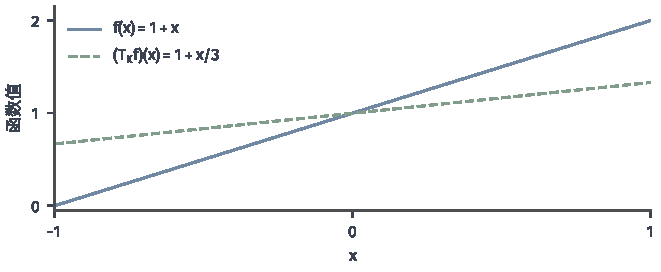
\includegraphics[width=112mm]{figures/01-mathematical-preliminaries-upper/02-linear-algebra-and-geometry/matplotlib/comprehension-additions/functional-integral-operator-action.pdf}
  \caption{$K(x,z)=1+xz$、$\mathrm d\mu=\mathrm dz/2$下，$f(x)=1+x$（实线）与其积分像$(T_Kf)(x)=1+x/3$（虚线）。积分把斜率压到原来的$1/3$，常数分量不动：正特征值$1$与$1/3$分别作用在常数与线性方向上。}
  \label{fig:vol1-add-functional-integral-operator-action}
\end{figure}

在归一测度下算谱。$T_K1=\int1\,\mathrm d\mu=1$，故$\psi_1=1$、$\mu_1=1$；$T_Kx=\int z\,\mathrm d\mu+x\int z^2\,\mathrm d\mu=x/3$，故$\psi_2=\sqrt3\,x$（归一：$\int 3x^2\,\mathrm d\mu=1$）、$\mu_2=1/3$。其余与$1,x$正交的方向属于零空间；两个正谱方向只覆盖仿射子空间，不能说整个$L^2[-1,1]$只有两个方向。

对$f=a+bx$，谱系数$b_1=\langle f,\psi_1\rangle=a$、$b_2=\langle f,\psi_2\rangle=b/\sqrt3$，故
\begin{equation}
\label{eq:functional-affine-two-norms}
\|f\|_{L^2(\mu)}^2=a^2+\frac{b^2}{3},\qquad
\|f\|_{H_K}^2=\frac{b_1^2}{\mu_1}+\frac{b_2^2}{\mu_2}=a^2+b^2.
\end{equation}
取$f=1+x$时两者分别为$4/3$和$2$；截到常数方向的尾误差平方分别为$1/3$和$1$，可与上面两种尾误差逐项核对。该谱例沿用前面同一仿射核空间，但额外加入测度后才取得积分特征值；改变测度会改变积分谱与$L^2$归一方向，不会自动改变原核通过再生关系定义的内积。

\subsection{积分方程的迭代求解}
\label{subsec:integral-equation-iteration}

前面给定函数计算积分输出；这里改为给定积分规则和外部项，寻找满足方程的未知函数。两项围绕同一名义方程，仅改变更新是否精确执行；表示截断与惩罚参数极限归入各自任务，不在这里混用。

\subsubsection{自映射与压缩条件}
\label{subsubsec:self-map-contraction}

固定$g\in C([a,b])$、紧矩形$[a,b]\times[a,b]$上连续的实核$K$与参数$\lambda$，要求未知函数$f\in C([a,b])$满足第二类Fredholm积分方程
\begin{equation}
\label{eq:functional-fredholm-equation}
f(x)=g(x)+\lambda\int_a^b K(x,t)f(t)\,\mathrm dt.
\end{equation}
把右端记为$Tf$：积分部分是线性算子，加入固定$g$后$T$是仿射映射。目标是求解该方程，即找$T$的不动点，而不只是生成一条没有解释对象的函数序列。

先核对$T$确实把$C([a,b])$映回自身。$K$在紧矩形上联合连续，故有界且一致连续。对固定连续$f$，
\[
|Tf(x)-Tf(z)|\le|g(x)-g(z)|+|\lambda|\|f\|_\infty\int_a^b|K(x,t)-K(z,t)|\,\mathrm dt;
\]
右端两项随$|x-z|\to0$一致趋于零，故$Tf$连续。$C([a,b])$在一致范数$\|\cdot\|_\infty$下完备。

接下来需要一个不动点存在定理，即\term{压缩映射}定理。它在本章本地完整建立，而不是引用别处结论。

\begin{theorem}[压缩映射定理（Banach不动点）]
\label{thm:banach-fixed-point}
设$(X,d)$为完备度量空间，$T:X\to X$满足压缩条件：存在$0\le q<1$使
\[
d(Tu,Tv)\le q\,d(u,v)\qquad(\forall u,v\in X).
\]
则$T$存在唯一不动点$x_*$。任取初值$x_0$，迭代$x_{k+1}=Tx_k$收敛于$x_*$，且
\begin{equation}
\label{eq:functional-iteration-apriori}
d(x_k,x_*)\le\frac{q^k}{1-q}\,d(x_1,x_0),
\end{equation}
\begin{equation}
\label{eq:functional-iteration-aposteriori}
d(x_k,x_*)\le\frac{q}{1-q}\,d(x_k,x_{k-1})\qquad(k\ge1).
\end{equation}
\end{theorem}

\begin{proof}
压缩映射连续：$d(Tx,Ty)\le q\,d(x,y)\to0$。逐步递推给出相邻步误差
\[
d(x_{n+1},x_n)\le q\,d(x_n,x_{n-1})\le\cdots\le q^n d(x_1,x_0).
\]
对$m>n$用三角不等式与几何级数，
\[
d(x_m,x_n)\le\sum_{j=n}^{m-1}d(x_{j+1},x_j)
\le d(x_1,x_0)\sum_{j=n}^{m-1}q^j
\le\frac{q^n}{1-q}d(x_1,x_0)\to0.
\]
$(x_n)$是Cauchy列；$X$完备，$x_n\to x_*$。由$T$连续，$Tx_*=\lim Tx_n=\lim x_{n+1}=x_*$，不动点存在。

唯一性：若$x_*,y_*$均为不动点，$d(x_*,y_*)=d(Tx_*,Ty_*)\le q\,d(x_*,y_*)$，$q<1$迫使$d(x_*,y_*)=0$。

先验界：在上面的逐步递推中令$m\to\infty$，
\[
d(x_*,x_n)\le\frac{q^n}{1-q}d(x_1,x_0).
\]
后验界：$d(x_n,x_*)\le q\,d(x_{n-1},x_*)$，故
\[
d(x_{n-1},x_*)\le d(x_{n-1},x_n)+d(x_n,x_*)\le d(x_{n-1},x_n)+q\,d(x_{n-1},x_*),
\]
整理得$(1-q)d(x_{n-1},x_*)\le d(x_{n-1},x_n)$，即$d(x_n,x_*)\le\frac{q}{1-q}d(x_n,x_{n-1})$。
\end{proof}

回到积分方程。对任意$f,h\in C([a,b])$，先在积分内作差再取绝对值，
\[
|Tf(x)-Th(x)|\le|\lambda|\|f-h\|_\infty\int_a^b|K(x,t)|\,\mathrm dt,
\]
故
\[
\|Tf-Th\|_\infty\le q\|f-h\|_\infty,\qquad
q=|\lambda|\sup_{x\in[a,b]}\int_a^b|K(x,t)|\,\mathrm dt.
\]
$q$必须对所有输入函数统一且满足$q<1$，不能用某次更新恰好变小代替严格压缩条件。自映射、完备与统一$q<1$齐备，定理\ref{thm:banach-fixed-point}给出唯一不动点$f_*$；由$T$的定义式，$f_*$正是方程\eqref{eq:functional-fredholm-equation}的解。

\subsubsection{精确更新与执行误差}
\label{subsubsec:exact-inexact-updates}

\paragraph{精确迭代的收敛与停止误差}

固定同一$g,K,\lambda$及初值$f^{(0)}\in C([a,b])$，令$f^{(k+1)}=Tf^{(k)}$。由刚核对的条件，精确迭代在一致范数中趋向唯一解$f_*$；方程与名义更新映射不变，变化的只是迭代中的近似函数。

先验界\eqref{eq:functional-iteration-apriori}说明误差只需初始更新差$\|f^{(1)}-f^{(0)}\|_\infty$与预先取得的$q$估计；后验界\eqref{eq:functional-iteration-aposteriori}说明已算出的相邻差$\|f^{(k)}-f^{(k-1)}\|_\infty$可直接用于停止判断。$q$接近一时必须保留$1/(1-q)$的放大因子：相邻变化小不直接等于误差同样小。$q\ge1$只使压缩论证失去保证，并不推出积分方程无解或多解；若要继续，须用别的条件另证。

\paragraph{同一方程下的扰动迭代}

保持同一名义$T$，实际更新未必精确执行：设
\[
\|f^{(k+1)}-Tf^{(k)}\|_\infty\le\eta_k,
\]
记$e_k=\|f^{(k)}-f_*\|_\infty$。先以三角不等式分离执行误差与名义输出差，再用压缩条件，
\begin{equation}
\label{eq:functional-perturbed-iteration}
e_{k+1}
\le\|f^{(k+1)}-Tf^{(k)}\|_\infty+\|Tf^{(k)}-Tf_*\|_\infty
\le\eta_k+q\,e_k.
\end{equation}
$\eta_k$可表示数值积分与更新造成的、对更新后整个函数的一致偏差，但不能把未经比较的模型差异也塞入其中。

反复展开递推：
\begin{equation}
\label{eq:functional-perturbed-unrolling}
e_k\le q^k e_0+\sum_{j=0}^{k-1}q^{\,k-1-j}\eta_j.
\end{equation}
初值影响随迭代按$q^k$衰减；历次执行误差按剩余更新次数加权。若$\eta_j\le\eta$一致，几何级数给出
\[
\limsup_{k\to\infty}e_k\le\frac{\eta}{1-q}.
\]
这是持续执行误差造成的误差地板上界，不保证每条轨迹收敛，更不保证误差恰好达到该边界。

若$\eta_j\to0$，把误差和分为有限早期项与尾部：对固定$J$，$j\le J$的有限项因几何权重$q^{k-1-j}\to0$而消失；$j>J$的尾部由$\sup_{j>J}\eta_j$乘$1/(1-q)$控制。取$J$足够大使尾部界任意小，再令$k\to\infty$，即得$e_k\to0$。更一般的可求和条件可作为同一分解的充分情形。比较持续与衰减执行误差时始终固定方程、初值和名义$q$，改变的仅是执行精度。若实际近似函数不在所定连续空间中，或自映射、完备、严格压缩任一项缺失，都须重建适用框架；这些限制与$q\ge1$的边界共同保留。
\section{泛函变分与函数拟合}
\label{sec:variational-functional-fitting}

前面各节把函数作为已知对象，研究怎样合法地读取它、用它构造算子或把它分解成正交方向。本节把函数改为未知量：候选函数本身是优化变量，我们要在给定候选空间、给定观测数据和给定偏差计量下，判断最优函数是否存在、是什么形状、对数据扰动有多敏感。三个任务分别规定不同的观测类型：有限个线性读数、整个定义域上的目标函数值，以及希望逼近的梯度向量场。变分提供这些任务共用的扰动语言——用$f+th$代替整条函数并考察目标的一阶变化；观测类型不同，可行扰动和残差计价就不同。不同任务也可以组合，例如同时拟合函数值和梯度场，但组合时必须写出共同候选空间、完整目标和各项权重，不能仅凭惩罚名称判断任务。

本节把每个拟合任务的识别、计算、数据扰动和参数极限放在相应问题内分别回答。一次最优化是否达到下确界、最优函数是否唯一、系数是否唯一、迭代算法是否收敛，是四个不同的判断；改变数据、改变惩罚参数与增加计算次数也不是同一个极限，后面凡涉及“收敛”或“稳定”都指明固定了什么、改变了什么。

\subsection{泛函微分与最优条件}
\label{subsec:functional-differential-optimality}

先在给定函数空间中说明怎样改变整条函数并计量目标的一阶响应，随后把同一扰动语言用于抽象目标和积分目标。微分只给出一阶变化的线性读数；最优条件还要考虑哪些扰动在当前候选下可行；这些条件本身是驻点刻画，不保证最小值达到，也不替代存在性证明。

\subsubsection{方向导数、Fréchet微分与梯度}
\label{subsubsec:frechet-gradient}

\paragraph{从函数扰动到有界线性微分}

固定实Hilbert空间$H$，其内积与范数分别记作$\langle\cdot,\cdot\rangle_H$与$\|\cdot\|_H$，令$J:H\to\mathbb R$在$f$的某个开邻域内取有限实值。先把“对函数求导”与熟悉的“对输入位置求导”分开：$f'(x)$描述函数值随位置$x$的变化，这里固定整条函数$f$不动，让它作为一个整体沿某个方向$h\in H$移动，考察目标值的响应。取实数$t$，用$f+th$改变整条函数，在固定$h$时定义
\[
  \mathrm d_hJ(f)
  =\lim_{t\to0}\frac{J(f+th)-J(f)}{t};
\]
这个极限称为$J$在$f$沿方向$h$的\term{方向导数}。它回答“目标对函数沿$h$的微小整体变化有多敏感”，与$f'(x)$是两类不同的微分。

逐个方向固定$h$取极限，只能核对“每条射线方向上目标都有线性响应”，不能控制许多方向同时变化时小扰动的合力。这正如有限维中各方向偏导数存在不保证可微：方向导数沿离散方向都存在，仍可能在斜向上突然失效。为此要求一个统一的一阶近似：存在一个有界线性泛函$DJ(f):H\to\mathbb R$，使$h$足够小时
\begin{equation}
  J(f+h)=J(f)+DJ(f)[h]+r_f(h),\qquad
  \frac{|r_f(h)|}{\|h\|_H}\to0\quad(\|h\|_H\to0).
  \label{eq:functional-frechet-differential}
\end{equation}
\begin{definition}[方向导数与Fréchet微分]\label{def:functional-frechet}
设$H$为实Hilbert空间，$J$在$f$附近有限。若对一切$h\in H$方向导数存在，则称$J$在$f$处有方向导数；若还存在有界线性泛函$DJ(f)$使式~\eqref{eq:functional-frechet-differential}的余项满足$|r_f(h)|/\|h\|_H\to0$，则称$J$在$f$处Fréchet微分可微，$DJ(f)$为其Fréchet微分（亦称\term{Fréchet导数}）。
\end{definition}
余项条件是对所有趋零扰动同时提出的：它要求余项比任意一阶位移都更小，而不是逐方向分别趋零。因此，每个方向导数存在并不直接推出Fréchet可微；要拿到统一估计，还须另行证明。

Fréchet微分$DJ(f)$是有界线性泛函，输出只是一个数。第~\ref{subsubsec:riesz-representation}节已经证明，实Hilbert空间中每个有界线性泛函$L$都唯一对应一个方向$h_L$使$L(h)=\langle h,h_L\rangle_H$。把这个结论用于$DJ(f)$，存在唯一的$\nabla_HJ(f)\in H$使
\[
  DJ(f)[h]=\langle\nabla_HJ(f),h\rangle_H,
\]
称$\nabla_HJ(f)$为$J$在$f$处关于内积$\langle\cdot,\cdot\rangle_H$的\term{梯度}。微分与梯度由此分开：微分对扰动输出标量读数，梯度是在当前内积下表示这个读数的那个空间方向；更换内积会更换代表方向，却不更换微分本身。不能把这两个对象当成同一个公式名称，也不能脱离内积谈“梯度就是微分”。

\paragraph{改变内积时的梯度}

下面用一个可逐项复算的例子核对微分、余项与梯度的关系，并直接观察“微分不变、梯度随内积改变”。取仿射函数空间
\[
  H=\{f:x\mapsto a+bx:a,b\in\mathbb R\},
\]
它是维数为二的实Hilbert空间。在这个空间上定义目标
\[
  J(f)=\frac{a^2+b^2}{2}.
\]
对任意扰动$h(x)=u+vx$，展开
\[
\begin{aligned}
  J(f+th)
  &=\frac{(a+tu)^2+(b+tv)^2}{2}\\
  &=J(f)+t(au+bv)+\frac{t^2(u^2+v^2)}{2}.
\end{aligned}
\]
因此沿$h$的方向导数为$au+bv$，且余项$r_f(th)=t^2(u^2+v^2)/2$满足
\[
  \frac{|r_f(th)|}{\|th\|_H}\to0
\]
只要所选范数等价于系数欧氏范数。线性部分$DJ(f)[h]=au+bv$与所选内积无关；它是否Fréchet可微，由余项比一阶位移更小这一条件核对，上式同时给出了线性部分和余项的量级。

第一种内积取系数内积
\[
  \langle a+bx,u+vx\rangle_1=au+bv.
\]
此时直接看出$\nabla_{H,1}J(f)=a+bx$，因为$\langle a+bx,u+vx\rangle_1=au+bv=DJ(f)[h]$。

第二种内积改用$[-1,1]$上$\mathrm d\mu=\mathrm dx/2$的$L^2$内积。逐项积分：
\[
\begin{aligned}
  \langle a+bx,u+vx\rangle_2
  &=\int_{-1}^1(a+bx)(u+vx)\,\frac{\mathrm dx}{2}\\
  &=au\int\frac{\mathrm dx}{2}
  +(av+bu)\int x\,\frac{\mathrm dx}{2}
  +bv\int x^2\,\frac{\mathrm dx}{2}\\
  &=au+\frac{bv}{3},
\end{aligned}
\]
其中奇函数项在对称区间上积分为零，$\int x^2\,\mathrm dx/2=1/3$。要求梯度$g(x)=\alpha+\beta x$满足
\[
  \langle g,u+vx\rangle_2=\alpha u+\frac{\beta v}{3}=au+bv
  \]
对所有$u,v$成立，解得$\alpha=a$、$\beta=3b$，即
\[
  \nabla_{H,2}J(f)=a+3bx.
\]
两种内积在这个有限维空间里拓扑等价，目标$J$和微分$DJ(f)[h]=au+bv$都没有改变，改变的只是表示该读数的空间方向。这个例子为后面区分“目标变化”与“优化几何变化”提供可复算的依据：同一个$J$，在系数内积下沿$(1,0)$走一步最陡，在$L^2$内积下最陡方向的系数变成$(1,3)$。

\subsubsection{可行扰动、最优条件与梯度流}
\label{subsubsec:feasible-optimality-flow}

\paragraph{凸约束下的一阶条件}

无约束时可以沿$+h$和$-h$两个方向试走；候选集$C$为凸集但不含内点时，边界上的候选可能只允许向一侧移动，因此一阶条件必须按“哪些扰动可行”来表述。

给定非空\term{凸集}$C\subset H$：对任意$f_1,f_2\in C$，线段$(1-t)f_1+tf_2$（$0\le t\le1$）也在$C$中。设$f_*\in C$是$J$在$C$上的最小点，对任意$g\in C$，凸性保证
\[
  f_*+t(g-f_*)\in C,\qquad 0\le t\le1.
\]
因为$f_*$最小，对$t>0$有$J(f_*+t(g-f_*))\ge J(f_*)$。若$J$在$f_*$Fréchet可微，令$t\downarrow0$，由方向导数的定义得到
\begin{equation}
  DJ(f_*)[g-f_*]\ge0,\qquad\forall g\in C.
  \label{eq:functional-convex-optimality}
\end{equation}
这就是最小点必须满足的一阶条件。注意这里$g-f_*$只能沿从$f_*$指向$C$内部的方向取；在边界附近不能任取正负扰动，否则会跑出候选集。

在这个必要条件之上加凸性，可以取得充分性。

\begin{theorem}[凸候选集上的一阶最优条件]\label{thm:functional-convex-optimality}
设$C\subset H$非空凸，$J$在$C$上凸，且在$f_*\in C$的开邻域内Fréchet可微。则$f_*$是$J$在$C$上的最小点，当且仅当
\[
  DJ(f_*)[g-f_*]\ge0,\qquad\forall g\in C.
\]
\end{theorem}

\begin{proof}
必要性已在上面给出：最小点向任意可行方向的一阶响应不能为负。

充分性使用\term{凸函数}的一阶下界：对凸且Fréchet可微的$J$，有
\[
  J(g)\ge J(f_*)+DJ(f_*)[g-f_*],\qquad\forall g\in C.
\]
（这是一维凸函数切线不等式$\varphi(t)\ge\varphi(0)+\varphi'(0)t$在Hilbert空间中的版本，由$J(f_*+t(g-f_*))$关于$t$的凸性对$t\ge0$展开取得。）再由条件$DJ(f_*)[g-f_*]\ge0$，右端不小于$J(f_*)$，即$J(g)\ge J(f_*)$对所有$g\in C$成立。
\end{proof}

定理先说明“最小点必有此不等式”（必要性），再增加凸性取得“满足此不等式即全局最优”（充分性）。存在性、严格凸时的至多唯一性、以及最小者实际是否达到，仍是另外的问题：本定理不证明下确界被取得，也不把驻点条件推广到非凸目标。

\paragraph{梯度流的能量变化及边界}

在无约束$H$上，沿梯度方向下降是最熟悉的一阶迭代语言。设曲线$f(t)$对$t$可微，且$J$可用链式法则求复合导，定义梯度流
\[
  \dot f(t)=-\nabla_HJ(f(t)).
\]
把链式法则写成一阶响应的形式：
\[
  \frac{\mathrm d}{\mathrm dt}J(f(t))
  =DJ(f(t))[\dot f(t)].
\]
代入$\dot f=-\nabla_HJ(f)$，由Riesz表示$DJ(f)[\nabla_HJ(f)]=\langle\nabla_HJ(f),\nabla_HJ(f)\rangle_H=\|\nabla_HJ(f)\|_H^2$，得到能量恒等式
\[
  \frac{\mathrm d}{\mathrm dt}J(f(t))
  =-\|\nabla_HJ(f(t))\|_H^2\le0.
\]
这说明了为什么该方向使目标下降：每一步的一阶响应恰好是梯度范数的平方。但这个恒等式只是在一条已经存在的解曲线上核算能量变化，并不是解曲线存在的证明；仅有下降还不足以推出全局存在性、轨迹收敛到某个函数、或收敛到全局最小者。此外，有约束候选$C$上不能直接套用这个无约束方程，须另给投影或可行保持机制；目标不可微时，须另用\term{次梯度}等适当条件。具体热演化方程的全局存在、收敛和长时间行为由后续微分方程章建立，本节只保留目标、梯度和能量变化的共同接口。

\subsubsection{积分泛函的内部条件与边界条件}
\label{subsubsec:integral-functional-variation}

\paragraph{局部密度的一阶变化}

前面的扰动语言不依赖$J$的具体形式。下面把它用于一类最重要的目标——逐点积分密度。设$\Omega\subset\mathbb R^d$为有界光滑域，$u:\Omega\to\mathbb R^r$可以有多个分量，$F:\Omega\times\mathbb R^r\times\mathbb R^{r\times d}\to\mathbb R$可以耦合各分量，考虑
\[
  J(u)=\int_\Omega F(x,u,\nabla u)\,\mathrm dx.
\]
先在$u,h,F$都足够光滑、且允许把导数移入积分的支配条件下计算一阶变化。对每个分量$u_a$及其梯度$\nabla u_a$作一阶展开：
\[
  F(x,u+h,\nabla u+\nabla h)
  =F(x,u,\nabla u)
  +\sum_a\left(F_{u_a}h_a+F_{\nabla u_a}\cdot\nabla h_a\right)+o(\|h\|_{C^1}),
\]
其中$F_{u_a}$是$F$对$u_a$的偏导，$F_{\nabla u_a}$是对该分量梯度的偏导向量。除以$t$并令$t\to0$（余项由支配条件一致地趋于零），得到
\begin{equation}
  \delta J(u)[h]
  =\int_\Omega\sum_a
  \left(F_{u_a}h_a+F_{\nabla u_a}\cdot\nabla h_a\right)\mathrm dx.
  \label{eq:functional-general-euler-lagrange-variation}
\end{equation}
光滑性和可移项条件不足时，不能把这个经典计算自动推广到任意Sobolev目标；那时应保留积分形式本身，而不把它点态化。

一阶变化由两部分组成。对梯度项作分部积分（高维用散度定理）：对每个分量$a$，把向量场$F_{\nabla u_a}h_a$的散度展开为$\operatorname{div}(F_{\nabla u_a}h_a)=(\operatorname{div}F_{\nabla u_a})h_a+F_{\nabla u_a}\cdot\nabla h_a$，
\[
  \int_\Omega F_{\nabla u_a}\cdot\nabla h_a\,\mathrm dx
  =\int_{\partial\Omega}(F_{\nabla u_a}\cdot n)h_a\,\mathrm dS
  -\int_\Omega \operatorname{div}(F_{\nabla u_a})h_a\,\mathrm dx,
\]
其中$n$是$\partial\Omega$的单位外法向量；左边是被积分进去的梯度项，导数$\partial_i$全部落在$h_a$上。代入式~\eqref{eq:functional-general-euler-lagrange-variation}，一阶变化被分成内部项与边界项两部分：
\[
  \delta J(u)[h]
  =\int_\Omega\sum_a
  \left(F_{u_a}-\operatorname{div}F_{\nabla u_a}\right)h_a\,\mathrm dx
  +\int_{\partial\Omega}\sum_a
  \left(F_{\nabla u_a}\cdot n\right)h_a\,\mathrm dS.
\]
内部项只含扰动$h_a$本身，边界项只含$h_a$在边界上的迹。这一步说清了一阶变化的两个不同来源；后面判断驻点条件时，正是可行扰动的边界值决定两项各自由谁负责。

\paragraph{可行边界如何决定条件}

驻点要求$\delta J(u)[h]=0$对所有合法扰动$h$成立，而“合法”由候选集合规定。

若候选固定迹：$u$与$u+h$有相同的边界值$g=\operatorname{Tr}u$，则允许扰动的边界迹为零，边界项恒为零。此时内部项必须对所有$h$成立，由变分法基本引理（测试函数任意时积分恒为零迫使被积函数为零）取得内部条件
\[
  F_{u_a}-\operatorname{div}F_{\nabla u_a}=0,\qquad a=1,\ldots,r,
\]
即各分量的Euler--Lagrange方程。

若某个分量在边界上自由，该分量扰动的边界迹可以独立变化，则边界项独立地要求
\[
  F_{\nabla u_a}\cdot n=0\quad\text{在$\partial\Omega$上},
\]
这就是该分量的自然边界条件（自然通量为零）。混合边界要逐部分核对：固定迹处不重复要求自然通量，自由迹处才要求通量为零；把固定迹处也写上零通量是错误的，因为那里根本没有边界项负责。

当经典二阶导数或点态通量尚无意义时（候选只是Sobolev函数），应保留原来对所有合法测试扰动成立的一阶积分式~\eqref{eq:functional-general-euler-lagrange-variation}，而不是先点态化再谈散度。凸密度$F$在相应可积范围内使积分目标凸，配合仿射可行集（如固定迹的$G+H_0^1$），可以把上面的驻点条件用于充分性判断；非凸情形的唯一性与达到性仍需另证。下文梯度场拟合把各自密度代入这套运算，不再重复建立多分量框架。

\subsection{有限线性观测下的函数拟合}
\label{subsubsec:finite-observation-fitting}

现在进入具体的拟合任务。给定$n$个有界线性读取$L_i:H\to\mathbb R$及目标数值$y_i$，数据只约束$n$个读数。先检查这组数据是否相容、是否唯一确定候选；再说明单调不减的范数惩罚怎样消去数据看不见的方向；最后把函数目标化为有限参数问题。点值拟合只有在相应空间中点读数合法且有界时才属于这个范围——第~\ref{subsubsec:point-evaluation}节已经说明，在$L^2$等空间里点读数甚至不被范数控制。

\subsubsection{读数的相容性与可识别性}
\label{subsubsec:identifiability}

\paragraph{候选范围与不可见方向}

固定候选$C\subseteq H$和读数映射
\[
  L:f\mapsto(L_1f,\ldots,L_nf)\in\mathbb R^n.
\]
给定观测$y=(y_1,\ldots,y_n)^{\top}$，与之相容的候选集合为
\[
  \{f\in C:Lf=y\}.
\]
这个集合的非空性回答相容性：数据能否被某个候选达到。它恰有一个元素，回答的是“在这一组特定数据下候选是否唯一确定”。而$L$在整个$C$上的单射性要求更强：对所有可能的$y$，相容集合都至多有一个元素。这一单射性的准确表述是：任意两个相容候选之差不能落在零读数空间里，即$(C-C)\cap\ker L=\{0\}$；当$C$本身是线性子空间时，它才简化为$\ker L\cap C=\{0\}$。三者量词不同：相容性是“存在$f$使$Lf=y$”，数据下唯一是“恰有一个$f$”，映射单射是“一切$y$都至多一个$f$”；不能把针对一个$y$的判断替换成整个映射的单射性。

即使候选是有限维线性空间，也会因读取矩阵秩亏而不可识别。取$C=\{f(x)=a+bx\}$只读$f(0)$，数据$f(0)=a_0$确定系数$a$却不限制$b$，整条直线斜率任意。再看无限维例子：取两个函数
\[
  f(x)=0,\qquad g(x)=x(x^2-1),
\]
它们在$-1,0,1$三个位置都给出零读数，却是不同的函数；一般地，任何“在所有观测点为零”的多项式加到$g$上都不改变读数。图~\ref{fig:vol1-add-functional-unseen-observation-direction}画出了这种不可见方向。

\begin{figure}[!htb]
  \centering
  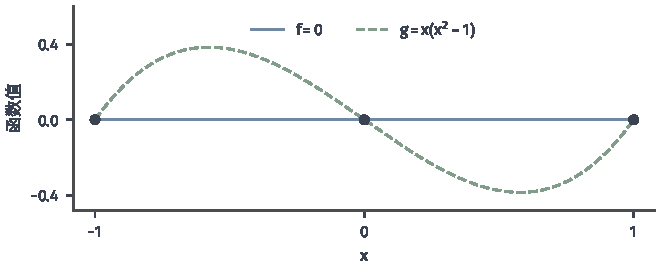
\includegraphics[width=112mm]{figures/01-mathematical-preliminaries-upper/02-linear-algebra-and-geometry/matplotlib/comprehension-additions/functional-unseen-observation-direction.pdf}
  \caption{有限点值留下不可见方向。定义域为$[-1,1]$，黑点为$x=-1,0,1$处的零读数。蓝线$f=0$与绿虚线$g(x)=x(x^2-1)$在三个位置完全一致，在其余位置可以不同。此处候选范围包含这些多项式；若另行限制次数或范数，仍须重新判断读取是否单射及候选是否可行。}
  \label{fig:vol1-add-functional-unseen-observation-direction}
\end{figure}

增加多项式次数、范数球或其他约束后，应在新的实际候选中重新检查哪些差函数仍可行：$g$不在新候选里，不可见方向就消失了。惩罚的作用是从同读数的多个函数中选定一个，它没有让原始数据获得额外识别能力——数据本身仍然看不见惩罚选定的方向。下一项用正交分解解释这种选择为什么能把搜索范围有限化。

\subsubsection{范数惩罚下的表示定理}
\label{subsubsec:representer-theorem}

\paragraph{用正交分解消去数据看不见的余项}

在实Hilbert空间$H$中取$n$个有界线性读取$L_i$。由第~\ref{subsubsec:riesz-representation}节的Riesz表示定理，每个$L_i$对应唯一方向$h_i\in H$使
\[
  L_i(f)=\langle f,h_i\rangle_H,\qquad i=1,\ldots,n.
\]
令
\[
  M=\operatorname{span}\{h_1,\ldots,h_n\}.
\]
$M$是有限维子空间；有限维子空间在Hilbert空间中闭（有限维空间上所有范数等价，柯西列必在该维数内收敛）。由第~\ref{subsubsec:orthogonal-projection}节的闭子空间投影结论，每个$f\in H$都有唯一正交分解
\[
  f=P_Mf+r,\qquad r\perp M,
\]
且$\|P_Mf\|_H\le\|f\|_H$。由$r\perp h_i$直接得到
\[
  L_i(r)=\langle r,h_i\rangle_H=0,\qquad i=1,\ldots,n,
\]
即余项$r$对全部读数不可见。这一步说明为什么去掉余项不改变数据项：不是“余项很小”，而是读数在$r$上恒为零。

现在考虑目标
\[
  J(f)=\Phi(Lf)+\Omega(\|f\|_H),
\]
其中$\Phi:\mathbb R^n\to\mathbb R$是读数代价，$\Omega:[0,\infty)\to\mathbb R$单调不减。因为$L_i(r)=0$，有$L(P_Mf)=Lf$，故$\Phi$两项相同；由$\|P_Mf\|_H\le\|f\|_H$及$\Omega$单调不减，得
\[
  J(P_Mf)=\Phi(Lf)+\Omega(\|P_Mf\|_H)
  \le\Phi(Lf)+\Omega(\|f\|_H)=J(f).
\]
于是在$M$中搜索与在全空间$H$中搜索取得相同下确界：任何$f$都被它的投影$P_Mf$（属于$M$）以不更差的目标取代。

\begin{theorem}[有限读取下的表示定理]\label{thm:functional-representer}
设$H$为实Hilbert空间，$L_1,\ldots,L_n$为有界线性读取，$h_i$为其Riesz方向，$M=\operatorname{span}\{h_i\}$。设
\[
  J(f)=\Phi(Lf)+\Omega(\|f\|_H),
\]
其中$\Phi$任意，$\Omega:[0,\infty)\to\mathbb R$单调不减。则：
\begin{enumerate}
  \item $\inf_{f\in H}J(f)=\inf_{f\in M}J(f)$；若$J$在$H$上达到最小值，则至少存在一个最小点属于$M$。
  \item 若$\Omega$还严格递增，且$J$达到最小值，则每个最小点都属于$M$。
  \item 若另有限制$C\subseteq H$代替全空间，上述结论在$P_M(C)\subseteq C$时成立；否则删除余项可能破坏可行性。
\end{enumerate}
\end{theorem}

\begin{proof}
对任意$f\in H$，上面已证$J(P_Mf)\le J(f)$且$P_Mf\in M$，故$\inf_{f\in M}J\ge\inf_{f\in H}J$，反向不等式由$M\subset H$直接得到，两端相等。若$f_*$是$H$上的最小点，则$J(P_Mf_*)\le J(f_*)$；又因$f_*$最小，$J(P_Mf_*)\ge J(f_*)$，故$P_Mf_*$也是最小点且属于$M$，本定理第一点成立。

若$\Omega$严格递增，且$f_*$的余项$r=f_*-P_Mf_*\ne0$，则$\|P_Mf_*\|<\|f_*\|$，由严格递增得$\Omega(\|P_Mf_*\|)<\Omega(\|f_*\|)$，从而$J(P_Mf_*)<J(f_*)$，与$f_*$最小矛盾；故$r=0$，即$f_*\in M$，本定理第二点成立。

有$C$限制时，$P_Mf$必须仍落在$C$中，上述投影取代才合法；第~3点的投影保持条件由此而来。
\end{proof}

注意定理没有说：下确界一定达到、最小函数唯一、或系数唯一。表示形式只是把搜索空间降到$M$，存在性与唯一性仍要由具体$\Phi,\Omega$另行判断。

\paragraph{惩罚含义与附加约束}

同为范数惩罚，$\Omega$所控制的对象由空间和范数的定义决定：$L^2$范数只累计函数值整体大小，整数阶Sobolev范数还累计规定阶弱导的整体大小，RKHS范数通过核截面同时控制点值稳定性和两点差，Lipschitz约束则直接限制函数随输入的变化幅度。不能笼统地把所有范数惩罚称为“让函数每点、每阶导数都同样平滑”。

点读取对应$h_i=K_{x_i}$（再生核截面，见第~\ref{subsubsec:point-evaluation}节），一般线性读取仍用各自的Riesz方向$h_i$；两者共用上面的证明，只是$h_i$的具体来源不同。附加约束方面，核范数球和仅依赖这组读数的约束可以逐项检查投影保持性$P_M(C)\subseteq C$，任意约束不可默认满足。完成这些条件后，才进入实际的有限参数目标。图~\ref{fig:representer-finite-readings-to-solver}把整个流程串起来。

\begin{figure*}[htbp]
  \centering
  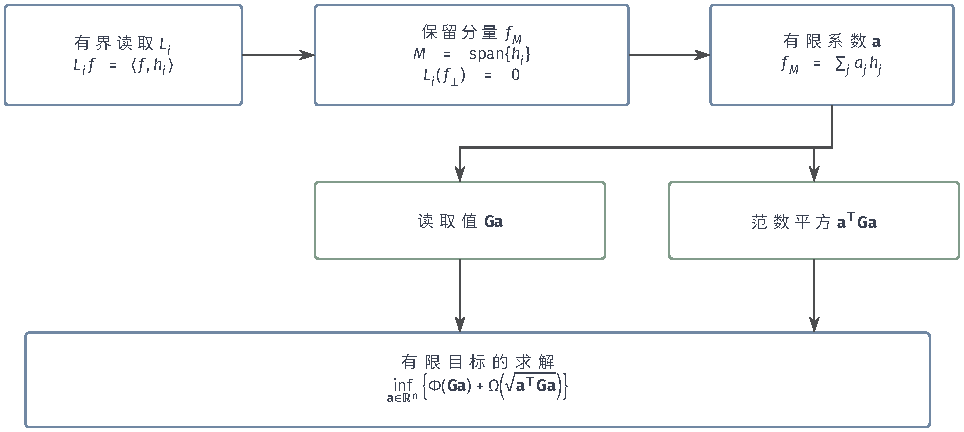
\includegraphics[width=163.258mm]{figures/01-mathematical-preliminaries-upper/02-linear-algebra-and-geometry/tikz/representer-finite-readings-to-solver/source.pdf}
  \caption{有限读取下的表示与求解。有界线性泛函$L_i$在Hilbert空间中有Riesz表示元$h_i$。所有读取只依赖$M=\operatorname{span}\{h_i\}$中的分量$f_M$，单调不减的范数惩罚允许删去$f_\perp$而不增大目标。写$f_M=\sum_j a_jh_j$后，读数与范数平方分别为$\bm G\bm a$与$\bm a^{\top}\bm G\bm a$。将这两个有限表达式代入目标后即可求解系数；最优解存在与系数唯一仍需另行判断。}
  \label{fig:representer-finite-readings-to-solver}
\end{figure*}

\subsubsection{Gram矩阵与平方拟合}
\label{subsubsec:gram-least-squares}

\paragraph{从函数目标到参数目标}

把$M$中的函数写成$f=\sum_{j=1}^n a_jh_j$，定义\term{Gram矩阵}
\[
  G_{ij}=\langle h_j,h_i\rangle_H=L_i(h_j),\qquad i,j=1,\ldots,n.
\]
逐项计算读数与范数：
\[
  (Lf)_i=L_i(f)=\sum_j a_jL_i(h_j)=\sum_jG_{ij}a_j,
\]
即$Lf=Ga$；以及
\begin{equation}
  \|f\|_H^2
  =\left\langle\sum_ja_jh_j,\sum_k a_kh_k\right\rangle_H
  =\sum_{i,j}a_iG_{ij}a_j=a^{\top}Ga.
  \label{eq:functional-finite-gram-objective}
\end{equation}
于是表示定理把目标化为有限变量$a\in\mathbb R^n$的问题：
\[
  \inf_{a\in\mathbb R^n}\left\{\Phi(Ga)+\Omega\!\left(\sqrt{a^{\top}Ga}\right)\right\}.
\]
只有读取恰好是点值$L_i(f)=f(x_i)$时，$G_{ij}=\langle K_{x_j},K_{x_i}\rangle_H=K(x_i,x_j)$才把$G$写成核矩阵；一般线性读取的Gram矩阵仍由$G_{ij}=\langle h_j,h_i\rangle$定义，不能省去“一般读数到核矩阵”这层条件。

取平方数据代价与二次范数惩罚，固定$\lambda>0$，考虑
\begin{equation}
  J_y(f)=\frac1n\sum_{i=1}^n(L_if-y_i)^2+\lambda\|f\|_H^2.
  \label{eq:functional-regularized-least-squares}
\end{equation}
代入有限表示$J_y(a)=\frac1n\|Ga-y\|_2^2+\lambda a^{\top}Ga$，对$a_j$求导：
\[
  \frac{\partial J_y}{\partial a_j}
  =\frac{2}{n}\sum_iG_{ij}(Ga-y)_i+2\lambda(Ga)_j.
\]
写成矩阵形式，驻点要求
\[
  \frac2nG(Ga-y)+2\lambda Ga=0,
\]
即
\[
  G\bigl[(G+n\lambda I)a-y\bigr]=0.
\]
注意$G$半正定：$a^{\top}Ga=\|\sum_ja_jh_j\|_H^2\ge0$。因此$G+n\lambda I$严格正定（其特征值为$t+n\lambda\ge n\lambda>0$），可逆。选取使括号内直接为零的规范代表
\begin{equation}
  a=(G+n\lambda I)^{-1}y.
  \label{eq:functional-tikhonov-representer}
\end{equation}
这里特意保留前一个驻点方程$G[(G+n\lambda I)a-y]=0$：后一个可逆方程只是选定代表，它要求括号向量本身为零；而驻点条件只要求该向量落在$\ker G$中，并未要求每组冗余系数都满足可逆方程。

为什么这个规范代表给出唯一的最优函数？先用前面已证的表示定理（定理~\ref{thm:functional-representer}）把搜索压到有限维。本问题的数据项$\Phi(z)=\frac1n\|z-y\|^2$凸，惩罚$\Omega(t)=\lambda t^2$随$t$严格递增；该定理已给出$\inf_{f\in H}J_y(f)=\inf_{f\in M}J_y(f)$，并且任何在$M$内达到下确界的点自动是$H$上的全局最小点。于是只需在$M$上证明最小值达到且唯一。

在$M$内写$f=\sum_ja_jh_j$，目标是系数$a\in\mathbb R^n$的二次函数$J_y(a)=\frac1n\|Ga-y\|^2+\lambda a^{\top}Ga$。把系数空间拆成$\ker G$与它的正交补：若$\delta a\in\ker G$，则$G\delta a=0$且$\delta a^{\top}G\delta a=0$，沿这个方向数据项与惩罚项都不变——系数冗余不改变函数，目标真正依赖的是$a$在$(\ker G)^\perp$上的投影$a_\perp$。退化情形先单独处理：若$\operatorname{rank}G=0$，则$G=0$；由$a^{\top}Ga=\|\sum_ja_jh_j\|_H^2$对一切$a$为零，迫使每个$h_i=0$，从而所有读数$L_if=\langle f,h_i\rangle\equiv0$恒为零，$M=\{0\}$。此时式~\eqref{eq:functional-regularized-least-squares}化为$J_y(f)=\frac1n\|y\|_2^2+\lambda\|f\|_H^2$，它随$\|f\|_H$严格增大，唯一最小点为$f_*=0$，最小代价为$\frac1n\|y\|_2^2$。以下设$\operatorname{rank}G\ge1$。在这个补空间上$G$严格正定：它是有限维对称矩阵，正特征值$t_i>0$全部出现，故有正的最小特征值$t_{\min}>0$。于是
\[
  J_y(a)\ge \lambda a_\perp^{\top}G a_\perp\ge \lambda t_{\min}\|a_\perp\|^2,
\]
右端随$\|a_\perp\|$增大而无界，目标在$(\ker G)^\perp$上强制。任取$c$，次水平集$\{a_\perp:J_y(a)\le c\}$一方面被$\|a_\perp\|\le\sqrt{c/(\lambda t_{\min})}$有界，另一方面是连续函数$J_y$的闭集；有限维闭且有界的集合必紧，由连续函数在紧集上达到极值的Weierstrass定理，$J_y$在$(\ker G)^\perp$上达到最小；$\ker G$方向任取零点，即得$M$上达到下确界的系数代表。

最后唯一性：数据项$\frac1n\|Lf-y\|^2$关于$f$凸，惩罚项$\lambda\|f\|_H^2$在$\lambda>0$时严格凸，故$J_y$在$H$上严格凸；严格凸函数至多有一个最小点，而最小点已在$M$内达到，故最小函数唯一。

\begin{theorem}[平方读取加二次惩罚的解]\label{thm:functional-tikhonov-solution}
设$H$为实Hilbert空间，$\lambda>0$，并给定$n$个有界线性读取
\[
  L_i:H\to\mathbb R,\qquad i=1,\ldots,n.
\]
则式~\eqref{eq:functional-regularized-least-squares}存在唯一的全局最小函数$f_*\in H$，且$f_*\in M=\operatorname{span}\{h_i\}$。其规范系数代表由式~\eqref{eq:functional-tikhonov-representer}给出：该代表在所有$h_i$方向满足一阶条件
\[
  DJ_y(f_*)[h_i]=0,
\]
在$M^\perp$方向上读数不变且$f_*$与扰动正交，一阶条件同样成立。
\end{theorem}

这里用具体二次目标完成了存在与唯一的证明，不能把这个结论反推给表示定理中任意的$\Phi,\Omega$。

\paragraph{函数唯一与系数冗余}

$G$奇异与最优函数唯一可以同时成立。若$\delta a\in\ker G$，则
\[
  \left\|\sum_j\delta a_jh_j\right\|_H^2
  =\delta a^{\top}G\,\delta a=0,
\]
由范数正定性，这个线性组合就是零函数；所有读数也都不变。因此问题不在函数层——最优函数唯一——而在坐标层：同一个函数$f_*=\sum_ja_j^*h_j$可以写成许多组系数，差向量都沿$\ker G$。

有附加约束时，先重查投影保持性$P_M(C)\subseteq C$，再把约束写成实际参数可行集。有限化只给出一个有限变量问题，不指定任何具体迭代算法都能收敛；下一项把“改变数据”和“增加计算次数”两种误差分别比较。

\subsubsection{数据扰动与计算误差}
\label{subsubsec:finite-fit-stability-computation}

\paragraph{固定惩罚参数时的数据稳定性}

固定$L_i,G,\lambda$，把观测数据从$y$改为$y+\delta y$，其余一切不动。规范代表的差为
\[
  \delta a=(G+n\lambda I)^{-1}\delta y.
\]
函数误差不能直接用系数欧氏距离$\|\delta a\|_2$计量——同一函数可有多组系数；正确的函数范数差是
\[
  \|\delta f\|_H^2=\delta a^{\top}G\,\delta a.
\]

把$G$正交对角化：$G=Q\operatorname{diag}(t_1,\ldots,t_n)Q^{\top}$，$t_i\ge0$。记$\tilde y=Q^{\top}\delta y$，则
\[
  \|\delta f\|_H^2
  =\sum_i\frac{t_i}{(t_i+n\lambda)^2}\,\tilde y_i^{\,2}.
\]
对每个$t\ge0$，由$(t+n\lambda)^2\ge4tn\lambda$（展开$t^2+2tn\lambda+n^2\lambda^2\ge4tn\lambda$即$(t-n\lambda)^2\ge0$）得
\[
  \frac{t}{(t+n\lambda)^2}\le\frac{1}{4n\lambda}.
\]
零特征方向$t=0$的权重为零，不贡献函数误差。合并得到
\begin{equation}
  \|\delta f\|_H\le\frac{\|\delta y\|_2}{2\sqrt{n\lambda}}.
  \label{eq:functional-data-stability-bound}
\end{equation}
这个界说明当前归一化$1/n$与固定的$\lambda$如何进入稳定常数。它比较的是两个不同数据任务的精确最优函数之差：没有研究任何求解算法，也没有让$\lambda$趋零。若随数据改变读取位置$x_i$或更换核，$G$本身也改变，就不能继续使用同一个矩阵逆的差分式~\eqref{eq:functional-tikhonov-representer}。

\paragraph{固定任务中的参数迭代}

现在固定同一数据目标$y$，只增加计算次数$k$。设迭代得到
\[
  f^{(k)}=\sum_i a_i^{(k)}h_i,
\]
最优规范代表为$a_*$。函数差的范数平方为
\[
  \|f^{(k)}-f_*\|_H^2
  =(a^{(k)}-a_*)^{\top}G(a^{(k)}-a_*).
\]
因此系数在$G$-内积意义下收敛足以推出函数收敛；有界读取再把函数收敛翻译成预测收敛。反向推断要小心：若$G$有零特征方向，系数沿$\ker G$改变时函数完全不变，所以“系数没怎么变”不保证函数没怎么变，“函数收敛”也不对应任何唯一的系数极限。因此停止条件必须说明检测的是参数、函数还是目标值。具体迭代算法的收敛仍需其光滑性、凸性和步长等条件，本节的表示定理不提供算法保证。

\subsection{整体函数值拟合}
\label{subsubsec:integral-error-fitting}

这里的数据不再是几个离散读数，而是整个定义域上的目标函数$y$：误差直接按积分范数在全体位置上累计。先处理Hilbert几何中“离目标最近的可行函数”这一纯几何问题，再处理RKHS候选与$L^2$观测之间的平方拟合；后者的解族极限和数据扰动放在同一任务内继续讨论，避免把不同范数、不同任务的结论分散使用。

\subsubsection{闭凸集合中的最近函数}
\label{subsubsec:nearest-closed-convex}

固定$f\in H$和非空闭凸集合$C\subset H$，研究
\[
  \inf_{g\in C}\|f-g\|_H.
\]
第~\ref{subsubsec:orthogonal-projection}节在闭子空间上证明过最近分量的存在唯一，那里$M$对线性组合封闭。现在$C$只是凸集，不再要求对线性组合封闭，但同一套估计仍然成立。

\paragraph{闭凸投影及其变分不等式}

\begin{theorem}[闭凸集上的最近点]\label{thm:functional-closed-convex-projection}
设$H$为实Hilbert空间，$C\subset H$非空闭凸。则存在唯一$g_*\in C$使$\|f-g_*\|_H=\inf_{g\in C}\|f-g\|_H$。
\end{theorem}

\begin{proof}
令$d=\inf_{g\in C}\|f-g\|_H$，取近似最小列$g_n\in C$使$\|f-g_n\|_H\to d$。凸性保证中点$(g_n+g_k)/2\in C$，故$\|f-(g_n+g_k)/2\|\ge d$。代入平行四边形恒等式
\[
  \begin{aligned}
    \|g_n-g_k\|^2
    &=2\|f-g_n\|^2+2\|f-g_k\|^2
      -4\left\|f-\frac{g_n+g_k}{2}\right\|^2\\
    &\le2\|f-g_n\|^2+2\|f-g_k\|^2-4d^2\to0,
  \end{aligned}
\]
$(g_n)$是柯西列。$H$完备给出极限$g_*$，$C$闭保留$g_*\in C$，范数连续性给出$\|f-g_*\|=d$。

若另有$g_{**}\in C$达到$d$，对它与$g_*$再用同一估计：
\[
  \|g_*-g_{**}\|^2
  \le2d^2+2d^2-4\left\|f-\frac{g_*+g_{**}}2\right\|^2
  \le4d^2-4d^2=0,
\]
故$g_*=g_{**}$。
\end{proof}

最近点$g_*$还可以用变分不等式刻画。沿可行方向$g_*+t(g-g_*)$（$0\le t\le1$，$g\in C$）展开：
\[
  \|f-g_*-t(g-g_*)\|^2
  =\|f-g_*\|^2-2t\langle f-g_*,g-g_*\rangle+t^2\|g-g_*\|^2.
\]
$t=0$是$t\ge0$上的最小，故一阶项非正：
\begin{equation}
  \langle f-g_*,g-g_*\rangle_H\le0,\qquad\forall g\in C.
  \label{eq:functional-convex-projection-characterization}
\end{equation}
反过来，若某个$g_*\in C$满足此不等式，则
\[
  \|f-g\|^2=\|f-g_*\|^2+\|g_*-g\|^2+2\langle f-g_*,g-g_*\rangle
  \ge\|f-g_*\|^2,
\]
故$g_*$确是最近点，条件充分。只有当$C$是闭线性子空间时，正负方向$g-g_*$都可行，不等式才加强为正交余项$\langle f-g_*,g\rangle=0$；一般凸集上只有单向变分不等式。

被最小化的整体误差由内积决定。若用Legendre、Chebyshev等方向作有限表示，区间变换的Jacobian及权重必须随内积重算；不能把换坐标后同一组系数的欧氏距离，当成原函数在$H$中的误差。

\subsubsection{RKHS平方拟合与谱收缩}
\label{subsubsec:rkhs-spectral-shrinkage}

\paragraph{明确两个空间并逐方向求解}

前面的最近点问题在单个Hilbert空间内进行。这里有两个空间：观测$y$在$L^2(\mu)$中累计，候选$f$在核Hilbert空间$H$中。沿用第~\ref{subsubsec:compact-spectrum-mercer}节给出的Mercer充分范围：紧度量输入域$X$、连续实对称半正定核$K$、有限正且全支撑的Borel测度$\mu$。在这些条件下，积分算子$T_K$在$L^2(\mu)$上紧自伴半正定，其归一特征方向$\psi_j$满足
\[
  T_K\psi_j=\mu_j\psi_j,\qquad \mu_j>0,
\]
且$\sqrt{\mu_j}\psi_j$构成$H$的完备正交系；$f=\sum_jb_j\psi_j\in H$当且仅当$\sum_jb_j^2/\mu_j<\infty$，且$\|f\|_H^2=\sum_jb_j^2/\mu_j$。固定该核的RKHS $H$与目标$y\in L^2(\mu)$，考虑
\begin{equation}
  J_\lambda(f)=\|f-y\|_{L^2(\mu)}^2+\lambda\|f\|_H^2,
  \qquad\lambda>0.
  \label{eq:functional-tikhonov-spectral-objective}
\end{equation}
$H\to L^2(\mu)$的有界性由再生关系和核对角上界$\sup_xK(x,x)<\infty$保证（紧集上连续核有界），两项积分因此都合法。只有当$\mu$总质量为一且相应观测解释成立时，才另外作统计解释；本节只作确定性拟合。

把$y$在$L^2(\mu)$中按$T_K$的谱分解：
\[
  y=y_0+\sum_jc_j\psi_j,\qquad y_0\in\ker T_K.
\]
对候选$f=\sum_jb_j\psi_j\in H$，$L^2$正交性把目标拆成互不耦合的方向：
\[
  J_\lambda(f)
  =\|y_0\|_{L^2}^2+\sum_j\left[(b_j-c_j)^2+\lambda\frac{b_j^2}{\mu_j}\right].
\]
零谱部分$y_0$没有可表示方向（$H$的元素只有正谱分量），它只贡献常数残差$\|y_0\|^2$；正谱部分则同时付出数据残差$(b_j-c_j)^2$与核范数代价$\lambda b_j^2/\mu_j$。

对每个正谱方向把括号配方：
\[
  (b_j-c_j)^2+\lambda\frac{b_j^2}{\mu_j}
  =\left(1+\frac{\lambda}{\mu_j}\right)
  \left(b_j-\frac{\mu_jc_j}{\mu_j+\lambda}\right)^2
  +\frac{\lambda c_j^2}{\mu_j+\lambda}.
\]
第一项系数$1+\lambda/\mu_j>0$，故逐方向唯一最小点为
\begin{equation}
  b_j^*=\frac{\mu_jc_j}{\mu_j+\lambda}.
  \label{eq:functional-spectral-shrinkage}
\end{equation}

这个式子目前只是形式候选：还要确认它确实给出$H$中的函数。由$\mu_j/(\mu_j+\lambda)^2\le1/(4\lambda)$（同一维均值不等式），
\[
  \sum_j\frac{(b_j^*)^2}{\mu_j}
  =\sum_j\frac{\mu_jc_j^2}{(\mu_j+\lambda)^2}
  \le\frac{1}{4\lambda}\sum_jc_j^2
  =\frac{\|y\|_{L^2}^2}{4\lambda}<\infty,
\]
故$f_*=\sum_jb_j^*\psi_j\in H$。目标值$\|y_0\|^2+\sum_j\lambda c_j^2/(\mu_j+\lambda)$是各项最小值之和，每个方向的配方都是严格凸二次，因此该候选达到唯一最小值。

\begin{theorem}[谱基下的正则化解]\label{thm:functional-spectral-shrinkage}
在上述Mercer范围与式~\eqref{eq:functional-tikhonov-spectral-objective}下，唯一最小函数为$f_*=\sum_j\frac{\mu_jc_j}{\mu_j+\lambda}\psi_j$，且$f_*\in H$。其$L^2$残差包含不可消除的零谱部分$\|y_0\|^2$。
\end{theorem}

\paragraph{表示误差与惩罚收缩}

回到仿射核算例核对方向。固定$X=[-1,1]$、$\mathrm d\mu=\mathrm dx/2$与$K(x,z)=1+xz$。第~\ref{subsubsec:compact-spectrum-mercer}节已算得归一方向$\psi_1=1$、$\psi_2=\sqrt3\,x$，正谱值$\mu_1=1$、$\mu_2=1/3$。收缩因子分别为
\[
  \frac{\mu_1}{\mu_1+\lambda}=\frac1{1+\lambda},
  \qquad
  \frac{\mu_2}{\mu_2+\lambda}=\frac{1/3}{1/3+\lambda}=\frac1{1+3\lambda},
\]
说明同一惩罚尺度$\lambda$对不同谱方向有不同收缩：小特征值方向被压得更狠。

取目标$y(x)=x^2$。它的正谱投影系数为
\[
  c_1=\langle x^2,\psi_1\rangle_{L^2(\mu)}=\int x^2\,\mathrm d\mu=\frac13,
  \qquad
  c_2=\langle x^2,\psi_2\rangle=\sqrt3\int x^3\,\mathrm d\mu=0,
\]
（$x^3$在对称区间积分为零），故$y=y_0+\frac13\psi_1$，$y_0=x^2-\frac13$。最优函数为
\[
  f_*=\frac{\mu_1c_1}{\mu_1+\lambda}\psi_1=\frac{1}{3(1+\lambda)}.
\]
零谱残差不可由任何$H$中函数表示：
\[
  \|y_0\|_{L^2}^2
  =\int\left(x^2-\frac13\right)^2\mathrm d\mu
  =\int x^4\,\mathrm d\mu-\frac23\int x^2\,\mathrm d\mu+\frac19
  =\frac15-\frac29+\frac19=\frac4{45}.
\]
另一类误差来自惩罚本身：$f_*$相对正谱投影$\frac13\psi_1$的收缩偏差为
\[
  \|f_*-\tfrac13\psi_1\|_{L^2}^2
  =\left(\frac{\lambda}{1+\lambda}\right)^2\frac19.
\]
表示残差$4/45$与收缩偏差不能合称为同一种拟合误差：前者由候选空间的谱覆盖不足造成，后者由惩罚选择造成。

令$\lambda=0$时，收缩消失，但$\sum_jc_j^2/\mu_j$可能发散，即正谱投影$P_+y$可能不属于$H$；此时下确界在$H$的闭包方向上达到，却没有$H$内最小函数。若另加范数球或额外点值约束，各方向系数将被新约束耦合，不能先逐方向收缩再默认它满足所有新约束。下一项在保持原任务条件时研究$\lambda$的解族。

\subsubsection{正则化参数的极限与有效维度}
\label{subsubsec:regularization-effective-dimension}

\paragraph{同一数据下的解族极限}

固定$y,K,\mu$，只改变$\lambda$，比较每个$\lambda$对应的精确解$f_\lambda$。由式~\eqref{eq:functional-spectral-shrinkage}，解相对正谱投影$P_+y=\sum_jc_j\psi_j$的$L^2$误差为
\[
  \|f_\lambda-P_+y\|_{L^2}^2
  =\sum_j\left(\frac{\lambda}{\mu_j+\lambda}\right)^2c_j^2.
\]
每一项随$\lambda\downarrow0$趋零，且被可求和的$\sum_jc_j^2=\|y\|^2_{L^2}$控制。按段取极限：先控制有限个前段（有限个数列逐项趋零），再用公共控制量$c_j^2$估计共同小的尾部（每一项$\le c_j^2$，尾和随$j$截断一致地小），取得
\[
  f_\lambda\to P_+y\quad\text{于 }L^2(\mu),\qquad\lambda\downarrow0.
\]
注意零谱残差$y_0$始终存在：$f_\lambda\to P_+y$而不是$y$，差$\|y_0\|$不可消除。

若正谱目标本身属于$H$，即$\sum_jc_j^2/\mu_j<\infty$，则在加权和中重复前段及尾部论证，可得$f_\lambda\to P_+y$于$H$范数。若该加权和发散，则
\[
  \|f_\lambda\|_H^2
  =\sum_j\frac{\mu_jc_j^2}{(\mu_j+\lambda)^2}
\]
随$\lambda\downarrow0$单调增至无穷（每项随$\lambda$减小而增大，由单调收敛定理取极限即$\sum_jc_j^2/\mu_j=\infty$）。此时只能在$L^2$范数下说$f_\lambda$收敛，不能写成$H$内收敛；这解释了“数据拟合越来越好”与“解的核范数爆炸”为何同时发生。

当$\lambda\to\infty$，各收缩系数$\mu_j/(\mu_j+\lambda)\to0$，且被原$c_j$一致控制，同样的级数估计给出$f_\lambda\to0$于$L^2$。这两端的参数极限比较的是“不同$\lambda$下各自的精确解”，与固定任务上的计算迭代无关。

\paragraph{给定惩罚尺度下的谱有效维度}

对固定$\lambda>0$，用
\begin{equation}
  d_{\mathrm{eff}}(\lambda)=\sum_j\frac{\mu_j}{\mu_j+\lambda}
  \label{eq:functional-effective-dimension}
\end{equation}
软计数被惩罚保留的方向：$\mu_j\gg\lambda$的方向贡献接近一，$\mu_j\ll\lambda$的方向贡献接近零。先检查这个级数是否有限：迹类条件$\sum_j\mu_j<\infty$给出上界
\[
  d_{\mathrm{eff}}(\lambda)\le\frac1\lambda\sum_j\mu_j.
\]
当前Mercer范围（连续核在紧集上）提供该条件：
\[
  \sum_j\mu_j=\int K(x,x)\,\mathrm d\mu(x)<\infty.
\]
仅有紧正算子还不够：例如特征值$\mu_j=1/j$的紧算子，$\sum_j\mu_j=\infty$，软计数级数同样发散。

仿射核在$\lambda=1$时给出
\[
  d_{\mathrm{eff}}(1)=\frac1{1+1}+\frac{1/3}{1/3+1}=\frac12+\frac14=\frac34,
\]
而其代数维数仍为二。\term{有效维度}是给定尺度$\lambda$下的谱量，不是函数类的覆盖规模：函数类覆盖还需另给函数类、半径和距离，二者都不独自提供统计或优化保证。图~\ref{fig:vol1-add-functional-effective-dimension}给出这个软计数的直观图像。

\begin{figure}[!htb]
  \centering
  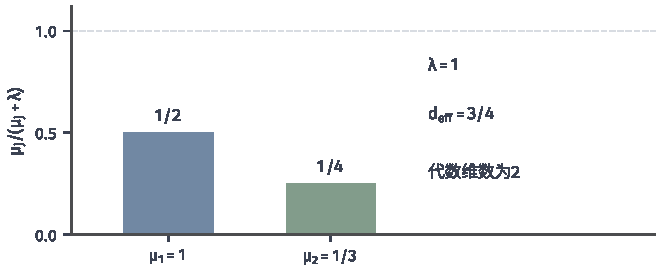
\includegraphics[width=112mm]{figures/01-mathematical-preliminaries-upper/02-linear-algebra-and-geometry/matplotlib/comprehension-additions/functional-effective-dimension-soft-count.pdf}
  \caption{有效维度按收缩比例计数。仿射核的两个正特征值为$1$和$1/3$，固定$\lambda=1$时，两个柱高分别为$1/(1+1)=1/2$与$(1/3)/(1/3+1)=1/4$，总和为$d_{\mathrm{eff}}=3/4$。灰虚线标记单一方向的完整贡献$1$，不表示另一项估计结果。}
  \label{fig:vol1-add-functional-effective-dimension}
\end{figure}

\subsubsection{固定参数下的数据稳定性}
\label{subsubsec:whole-fit-data-stability}

固定核、测度和$\lambda>0$，比较两个不同目标$y,\tilde y$对应的精确解$f_\lambda,\tilde f_\lambda$。对目标之差作相同的$L^2$谱分解：$y-\tilde y=\sum_j\delta c_j\psi_j$（零谱部分被消去），则解之差为
\[
  f_\lambda-\tilde f_\lambda=\sum_j\frac{\mu_j\delta c_j}{\mu_j+\lambda}\psi_j.
\]
按$L^2$范数计量，正谱系数乘上$\mu_j/(\mu_j+\lambda)\le1$，故
\[
  \|f_\lambda-\tilde f_\lambda\|_{L^2}
  \le\|y-\tilde y\|_{L^2}.
\]
这个结论比较同一算子的两项输入，$\lambda$全程固定，不让参数同时变化。

若按$H$范数计量输出，系数另带$1/\mu_j$权重：
\[
  \|f_\lambda-\tilde f_\lambda\|_H^2
  =\sum_j\frac{\mu_j\,\delta c_j^2}{(\mu_j+\lambda)^2}
  \le\frac{1}{4\lambda}\sum_j\delta c_j^2
  =\frac{\|y-\tilde y\|_{L^2}^2}{4\lambda},
\]
最后一步用$\mu_j/(\mu_j+\lambda)^2\le1/(4\lambda)$。于是
\begin{equation}
  \|f_\lambda-\tilde f_\lambda\|_H
  \le\frac{\|y-\tilde y\|_{L^2}}{2\sqrt\lambda}.
  \label{eq:functional-whole-fit-h-stability}
\end{equation}
换范数后常数从一变成$1/(2\sqrt\lambda)$，说明计量空间改变后实际改变了什么，而不是直接搬用前一段的系数一。

这里的数据稳定性、上一项的参数极限、以及有限任务中的算法误差各有各自的固定量与变化量：数据稳定性固定$K,\mu,\lambda$而改变$y$；参数极限固定$y,K,\mu$而改变$\lambda$；算法误差固定$y,K,\mu,\lambda$而增加迭代次数。一个任务既可能数据稳定又难以计算，也可能在$\lambda\downarrow0$时失去统一稳定常数，不能以其中一项代替另外两项。

\subsection{梯度场拟合与边界条件}
\label{subsubsec:gradient-field-fitting}

这里把观测从函数值改为向量场$v$：希望未知$u$的梯度接近$v$。固定有界连通Lipschitz域$\Omega\subset\mathbb R^d$，观测向量场$v\in L^2(\Omega;\mathbb R^d)$，已给提升$G\in H^1(\Omega)$与边界数据$g=\operatorname{Tr}G$（迹算子见第~\ref{subsubsec:trace-zero-boundary}节）。候选为
\[
  C=G+H_0^1(\Omega).
\]
残差是$\nabla u-v$；$v$未必是某个标量函数的精确梯度（例如环流场），因此不先假定残差可消为零，目标只能是“尽量小”。

\subsubsection{残差密度与可行扰动}
\label{subsubsec:residual-density-feasible}

在同一$v,g,C$上写残差密度的一般形式
\[
  J_\rho(u)=\int_\Omega\rho(\nabla u-v)\,\mathrm dx.
\]
二次密度$\rho_2(r)=\|r\|^2/2$与幅度型密度
\[
  \rho_\varepsilon(r)=\sqrt{\|r\|^2+\varepsilon^2}
\]
只改变残差的计价方式，不改变观测类型。它们可以与函数值项或有限读数项组合，但组合后必须重新写出完整目标、各项权重和共同候选，不能仅凭惩罚名称判断任务。

固定迹意味着允许扰动$h\in H_0^1(\Omega)$（边界迹为零）；若改为自由边界或均值约束，要先改变可行扰动集合，再使用共用的积分变分公式。$v=0$时上述两个密度才分别退化为纯梯度平方平滑与TV型平滑；没有其他观测或约束时，纯梯度平滑允许任意常量平移，不能说它自动保留信号。

\subsubsection{梯度残差的二次代价}
\label{subsubsec:quadratic-gradient-cost}

\paragraph{从二次目标到弱条件}

先取一维、$v=0$、固定端点的简单情形建立直觉：
\[
  J(f)=\frac12\int_0^1|f'|^2\,\mathrm dx.
\]
对光滑$f$和满足零端点条件的扰动$h$，展开
\[
  J(f+th)=\frac12\int|f'+th'|^2
  =J(f)+t\int f'h'\,\mathrm dx+\frac{t^2}{2}\int|h'|^2,
\]
故$DJ(f)[h]=\int f'h'\,\mathrm dx$。分部积分（$h$在端点为零，边界项消失）得$\int f'h'=-\int f''h$；由测试函数任意，驻点经典条件为$f''=0$，即仿射函数，再由固定端点值确定两个系数。一般$H^1$候选没有经典二阶导数时，先保留“对所有合法$h$成立”的积分条件$\int f'h'=0$，不强行点态化。注意这里是导数平方能量，要与二阶导数平方的弯曲能$\frac12\int|f''|^2$区别开：后者惩罚弯曲，前者惩罚斜率大小。

回到给定场$v\in L^2(\Omega;\mathbb R^d)$，取二次密度$\rho_2$（$v=0$时为$\frac12\int_\Omega\|\nabla u\|^2\,\mathrm dx$，即\term{Dirichlet能量}）：
\[
  J_2(u)=\frac12\int_\Omega\|\nabla u-v\|^2\,\mathrm dx.
\]
展开$J_2(u+th)-J_2(u)$的一次项（$h\in H_0^1$）：
\[
  t\int_\Omega(\nabla u-v)\cdot\nabla h\,\mathrm dx+o(t).
\]
故驻点弱式为
\begin{equation}
  \int_\Omega\nabla u\cdot\nabla h\,\mathrm dx
  =\int_\Omega v\cdot\nabla h\,\mathrm dx,
  \qquad\forall h\in H_0^1(\Omega).
  \label{eq:functional-guided-poisson-weak}
\end{equation}
当前$v\in L^2$和$u,h\in H^1$保证两边积分合法（Cauchy--Schwarz：$L^2$内$L^2$函数乘积可积）；即使$u$没有经典二阶导数，这个弱式仍保留。

在额外光滑条件下对左边分部积分，内部式解释为
\[
  \operatorname{div}(\nabla u-v)=0.
\]
自由边界处的自然通量是$(\nabla u-v)\cdot n$，一般不是齐次法向导数$\partial_nu=0$。若恰好$v=\nabla s$且$s\in H^1(\Omega)$，则$u-s$满足弱调和内部条件$\int\nabla(u-s)\cdot\nabla h=0$，边界差由修正项承担；任意$v$不必有这样的势$s$。

\paragraph{方程接口与求解边界}

这里的推导完成的是“候选与二次目标—可行一阶变化—弱方程”这条链路。带源Poisson方程、Poincaré不等式与Riesz表示下的存在唯一论证、自由边界的常量自由度以及源与通量相容条件，由后续微分方程章的Poisson弱解理论继续建立；本节不把当前驻点推导写成已经完成这些证明。连续弱问题存在唯一，也不能直接推出算法收敛或网格解逼近；具体五点系统及固定边界条件由五点差分承接，本章后面的连续能量离散节只检查已知函数的能量值和权重尺度，不替代解的数值分析。

\subsubsection{梯度残差的幅度代价}
\label{subsubsec:amplitude-gradient-cost}

\paragraph{正平滑参数下的一阶条件}

保留同一$v,g,C$，取$\varepsilon>0$及幅度型目标
\[
  J_\varepsilon(u)=\int_\Omega\sqrt{\|\nabla u-v\|^2+\varepsilon^2}\,\mathrm dx.
\]
先对残差向量$r=\nabla u-v$求密度导数：
\[
  \frac{\partial\rho_\varepsilon}{\partial r}
  =\frac{r}{\sqrt{\|r\|^2+\varepsilon^2}},
\]
再沿$\nabla h$用链式法则，得到一阶变化
\[
  \delta J_\varepsilon(u)[h]
  =\int_\Omega
  \frac{\nabla u-v}{\sqrt{\|\nabla u-v\|^2+\varepsilon^2}}
  \cdot\nabla h\,\mathrm dx.
\]
系数向量长度$\|\nabla u-v\|/\sqrt{\|\nabla u-v\|^2+\varepsilon^2}\le1$，被$|\nabla h|$一致支配，由控制收敛定理说明导数可以移入积分。令该一阶积分对全部合法$h\in H_0^1$为零，即得当前驻点弱条件；经典内部散度$\operatorname{div}\big((\nabla u-v)/\sqrt{\|\nabla u-v\|^2+\varepsilon^2}\big)=0$和自然边界通量，只在额外正则性或适用弱迹条件下解释。密度$\rho_\varepsilon$凸，故目标凸，但凸性不推出当前$H^1$候选中最小值达到或唯一，更不能沿用二次问题的Poisson线性形式。

\paragraph{零平滑参数、集中变化与BV边界}

当$\varepsilon=0$，残差为零处不能直接相除，应改用次梯度或变分不等式；$v=0$时密度退化为$\rho_0(r)=\|r\|$，即通常的\term{全变差}（TV）型平滑目标。用一个一维过渡比较两种密度对“集中变化”的响应：设$u$在宽度$\delta$内从高度$0$线性过渡到高度$a$，其余处斜率为零，则
\[
  \begin{aligned}
    \text{幅度积分}&=\int|u'|\,\mathrm dx=\frac{|a|}{\delta}\cdot\delta=|a|,\\
    \text{二次能量}&=\frac12\int|u'|^2\,\mathrm dx
      =\frac12\left(\frac a\delta\right)^2\delta=\frac{a^2}{2\delta}.
  \end{aligned}
\]
过渡收窄（$\delta\to0$）时幅度积分保持$|a|$不变，二次能量按$1/\delta$发散。二者对同一过渡的不同响应完全来自密度本身：幅度密度对“总变化量”计价，二次密度对“变化速率平方”计价。

一维中具有非零高度的跳跃不属于当前$H^1$候选（$H^1$函数在一维有绝对连续代表，不允许跳）。若要允许跳跃，必须以分布导数的测度表示进入BV空间并重新规定目标；本节只指出这条范围边界，不把BV存在理论混写成当前$H^1$结论。多维中逐坐标绝对值之和与逐点欧氏长度是不同密度，前者对方向的计价不同。即便密度逐点积分，共享的未知函数和边界约束仍耦合各位置，优化不能逐点独立；与其他观测项组合时，还须重新核对可微性、次梯度和可行保持条件。
\section{有限表示与函数逼近}
\label{sec:finite-representation-approximation}

本节固定目标函数、允许的定义域和误差尺度，研究怎样用有限个生成单元及其组合得到一个函数。前文的有限观测表示定理是在给定目标和惩罚下删除不可见方向；这里则主动选择近似族，并比较表示规模、局部修改和可达到的误差。“存在一个近似表示”只回答这个族是否足够丰富，不替代由有限读数识别目标、寻找参数的算法或学习保证。

下面固定一个共同目标
\[
  f_*(x)=\left|x-\frac12\right|,\qquad x\in[0,1],
\]
贯穿全节：多项式可以随次数增加而一致逼近它，含$1/2$结点的线性样条可以精确表示它，两个ReLU单元也可以精确表示它。这个对照比较的是同一个函数所需的构造条件，不从三个例子推断某种方案对所有目标都更省规模。生成单元的选择与多变量的组合方式是两个可以叠加的设计问题，下面分别讨论，不把它们写成互斥的函数类型。

\subsection{生成单元的选择}
\label{subsubsec:choice-of-generating-units}

下面固定同一个定义域与误差口径，分别考察全局多项式、局部分段直线、固定宽度的高斯核截面和神经单元怎样生成近似函数。四种方案各有自己的固定对象与可变规模：多项式的次数、样条的结点、高斯核的中心与项数、神经单元的宽度，分别随目标和精度变化，误差结论依赖的条件也随之不同。它们是几种有明确构造的方案，彼此可能存在表示联系；例如高斯核稠密性的证明借助多项式，却并不使高斯核截面成为多项式的一类。

\subsubsection{多项式逼近}
\label{subsubsec:polynomial-approximation}

对$[0,1]$上的连续目标$f$，先给一个可直接由网格读数形成的多项式，再证明它怎样控制全区间误差。结论中的次数可以随目标和精度增加，不固定一个有限维多项式空间后就宣称它能逼近所有连续函数。

在展开估计之前，先固定两个全程使用的对象。

\begin{definition}[连续模]
设$f$在区间$I$上有界。对$\delta>0$，定义
\[
  \omega_f(\delta)=\sup_{\substack{s,t\in I\\|s-t|\le\delta}}|f(s)-f(t)|.
\]
它是$f$在长度$\delta$的尺度上的最大振幅。$f$在紧区间上一致连续，等价于$\omega_f(\delta)\to0$（$\delta\downarrow0$）；若$f$还满足$|f(s)-f(t)|\le L|s-t|$，则有$\omega_f(\delta)\le L\delta$。
\label{def:functional-continuity-modulus}
\end{definition}

\paragraph{Bernstein多项式的构造}

固定整数$m\ge1$，在结点$j/m$读取$f$，定义
\begin{equation}
  B_mf(x)=\sum_{j=0}^{m}f\!\left(\frac jm\right)w_{m,j}(x),
  \qquad
  w_{m,j}(x)=\binom mjx^j(1-x)^{m-j}.
  \label{eq:functional-bernstein-polynomial}
\end{equation}
结点值是已知输入，$x$是求近似值的位置；每个权重都是$x$的多项式，因此结果仍是次数至多$m$的多项式。

把$m$个$x+(1-x)$的有限乘积按“选中$x$的次数”分组，得到
\[
  \sum_jw_{m,j}(x)=\bigl(x+(1-x)\bigr)^m=1;
\]
在$0\le x\le1$上各权重非负，因此$B_mf(x)$是结点值的凸组合。这一步只用有限乘积和二项式展开，不预先调用概率论。凸组合说明了取值范围，却还没有说明主要权重是否集中在靠近$x$的结点；下面把这个位置问题算成一组有限和恒等式。

\begin{lemma}[Bernstein权重的矩]
对$0\le x\le1$，上述权重满足
\[
  \sum_{j=0}^m w_{m,j}(x)=1,\qquad
  \sum_{j=0}^m j\,w_{m,j}(x)=mx,
\]
以及
\[
  \sum_{j=0}^m j(j-1)w_{m,j}(x)=m(m-1)x^2.
\]
进而有二阶中心矩恒等式
\begin{equation}
  \sum_{j=0}^m\left(\frac jm-x\right)^2w_{m,j}(x)
  =\frac{x(1-x)}m\le\frac1{4m}.
  \label{eq:functional-bernstein-second-moment}
\end{equation}
\end{lemma}

\begin{proof}
第一式已由二项式定理给出。对第二式，利用$j\binom mj=m\binom{m-1}{j-1}$，把求和下标改为$k=j-1$：
\[
  \sum_{j=0}^m j\,w_{m,j}(x)
  =mx\sum_{k=0}^{m-1}\binom{m-1}{k}x^k(1-x)^{m-1-k}
  =mx.
\]
对第三式，再用$j(j-1)\binom mj=m(m-1)\binom{m-2}{j-2}$（$m=1$时左边直接为零），类似地把下标改为$k=j-2$，得到
\[
  \begin{aligned}
  \sum_{j=0}^m j(j-1)w_{m,j}(x)
  &=m(m-1)x^2
    \sum_{k=0}^{m-2}\binom{m-2}{k}x^k(1-x)^{m-2-k}\\
  &=m(m-1)x^2.
  \end{aligned}
\]
最后用$j^2=j(j-1)+j$展开二阶中心矩：
\[
  \sum_j(j/m-x)^2w_{m,j}
  =\frac1{m^2}\sum_jj^2w_{m,j}-\frac{2x}{m}\sum_jj\,w_{m,j}+x^2\sum_jw_{m,j}.
\]
代入前两式，即得$(m(m-1)x^2+mx)/m^2-2x^2+x^2=x(1-x)/m$；再由$x(1-x)\le1/4$（$0\le x\le1$）得到右端上界$1/(4m)$。
\end{proof}

这个有限和恒等式的意义是：权重虽然散布在全部结点上，但离$x$较远的结点所占的总权重受$1/(4m)$控制，因而随$m$增大而衰减。

\paragraph{一致误差的估计}

\begin{theorem}[Bernstein--Weierstrass逼近]
设$f\in C([0,1])$，$B_mf$为式~\eqref{eq:functional-bernstein-polynomial}的Bernstein多项式。对任意$\delta>0$，
\begin{equation}
  \|B_mf-f\|_\infty
  \le\omega_f(\delta)+\frac{\|f\|_\infty}{2m\delta^2}.
  \label{eq:functional-bernstein-error}
\end{equation}
因而$\|B_mf-f\|_\infty\to0$（$m\to\infty$）。
\end{theorem}

\begin{proof}
固定$\delta>0$，用权重和为一把差写成
\[
  B_mf(x)-f(x)
  =\sum_{j=0}^m\left[f\!\left(\frac jm\right)-f(x)\right]w_{m,j}(x).
\]
把结点分成近处$|j/m-x|\le\delta$与远处$|j/m-x|>\delta$两组，这是同一个误差的两部分，并未另换目标或误差范数。

近处每个差值至多为连续模$\omega_f(\delta)$，而近处权重之和不超过$1$，故近处贡献不超过$\omega_f(\delta)$。

远处对每个$j$用$1\le(j/m-x)^2/\delta^2$放大权重，再由上面的矩恒等式控制总权重：
\[
  \sum_{|j/m-x|>\delta}w_{m,j}(x)
  \le\frac1{\delta^2}\sum_{j=0}^m\left(\frac jm-x\right)^2w_{m,j}(x)
  \le\frac1{4m\delta^2}.
\]
远处再用$|f(j/m)-f(x)|\le|f(j/m)|+|f(x)|\le2\|f\|_\infty$，得到远处贡献不超过$\|f\|_\infty/(2m\delta^2)$。两部分相加即得式~\eqref{eq:functional-bernstein-error}。

最后，$f$在紧区间$[0,1]$上一致连续，故任给$\varepsilon>0$可先选$\delta$使$\omega_f(\delta)<\varepsilon/2$；保持这个$\delta$，再取足够大的$m$使$\|f\|_\infty/(2m\delta^2)<\varepsilon/2$。两步缺一不可：仅知道某个固定$x$处误差趋零，不足以得出全区间共用的结论。
\end{proof}

回到折点目标$f_*$，本定理保证任意精度的一致多项式逼近，但任意一个多项式在$1/2$处都可微，不能与$f_*$在整个区间上完全相同。一般连续性也没有给出所有连续目标共用的快速速率；上面的速率$\omega_f(\delta)+C/(m\delta^2)$只说明收敛，常数随$\delta$的选择而变。下一个方案利用分段结构，在特定结点条件下直接表示这个折点。

\subsubsection{样条逼近}
\label{subsubsec:spline-approximation}

样条以分段多项式和指定结点衔接条件定义。这里先取最简单的连续分段直线，研究结点值怎样生成局部插值，以及结点变密怎样控制同一个连续目标的误差。

\paragraph{线性样条的构造与误差}

固定
\[
  0=t_0<t_1<\cdots<t_N=1,
\]
结点值$f(t_i)$及最大间距$h=\max_i(t_{i+1}-t_i)$。对$x\in[t_i,t_{i+1}]$写
\begin{equation}
  S_hf(x)=(1-s)f(t_i)+sf(t_{i+1}),
  \qquad s=\frac{x-t_i}{t_{i+1}-t_i}.
  \label{eq:functional-linear-spline}
\end{equation}
相邻区间在公共结点使用同一个读数，所以这个构造给出连续分段直线。要先区分“由全部样条组成的候选空间”与“由结点数据产生当前插值函数的操作”。

\begin{theorem}[线性样条的插值误差]
在上述记号下，若$f$在$[0,1]$上连续，则
\begin{equation}
  \|f-S_hf\|_\infty\le\omega_f(h).
  \label{eq:functional-spline-modulus-error}
\end{equation}
若再有$f\in C^2([0,1])$，则
\begin{equation}
  \|f-S_hf\|_\infty\le\frac{h^2}{8}\|f''\|_\infty.
  \label{eq:functional-spline-quadratic-error}
\end{equation}
\end{theorem}

\begin{proof}
在单元$[t_i,t_{i+1}]$上，由$(1-s)+s=1$把$f(x)-S_hf(x)$拆成
\[
  f(x)-S_hf(x)=(1-s)\bigl(f(x)-f(t_i)\bigr)+s\bigl(f(x)-f(t_{i+1})\bigr).
\]
两个端点离$x$都不超过$h$：$|x-t_i|=s(t_{i+1}-t_i)\le h$，$|x-t_{i+1}|=(1-s)(t_{i+1}-t_i)\le h$。故
\[
  |f(x)-S_hf(x)|\le(1-s)\omega_f(h)+s\omega_f(h)=\omega_f(h).
\]
对全部区间取上确界即得式~\eqref{eq:functional-spline-modulus-error}。若一列网格的最大间距$h\to0$，一致连续性使$\omega_f(h)\to0$，这些插值函数便一致趋于$f$；这个结论不要求网格等距。

为得到二阶速率，固定一个单元并考虑$g(x)=f(x)-S_hf(x)$。它在两端$t_i,t_{i+1}$处为零。对任意$x\in(t_i,t_{i+1})$，令
\[
  \lambda=\frac{g(x)}{(x-t_i)(x-t_{i+1})},
  \qquad
  G(u)=g(u)-\lambda(u-t_i)(u-t_{i+1}).
\]
函数$G$在$t_i,t_{i+1},x$三点处都为零。由Rolle定理，$G'$在这三点两两之间各有一个零点，共两个零点；再用一次Rolle定理，$G''$在单元内某点$\xi$处为零。注意$S_hf$在单元内是一次多项式，$S_h''=0$，而$((u-t_i)(u-t_{i+1}))''=2$，故
\[
  0=G''(\xi)=f''(\xi)-2\lambda,
  \qquad
  \lambda=\frac{f''(\xi)}2.
\]
代回$\lambda$的定义，得余项表示
\[
  f(x)-S_hf(x)=\frac{f''(\xi)}2(x-t_i)(x-t_{i+1}).
\]
在单元上$|(x-t_i)(x-t_{i+1})|\le\bigl((t_{i+1}-t_i)/2\bigr)^2\le h^2/4$，因而$|f(x)-S_hf(x)|\le h^2\|f''\|_\infty/8$。对单元取上确界即得式~\eqref{eq:functional-spline-quadratic-error}。新增的二阶导数条件支持更具体的速率，不能由一般连续性直接取得。
\end{proof}

\paragraph{样条的示例与局部修改}

\begin{example}[二次函数的两段插值]
对$f(x)=x^2$只取结点$0,1$，由端点值$0,1$得到$S_hf(x)=x$。函数$x-x^2$在$x=1/2$处取最大值$1/4$，故误差恰为$1/4$。此时$h=1$、$\|f''\|_\infty=2$，上一界$h^2\|f''\|_\infty/8=2/8=1/4$，二者吻合，可供核对余项估计中的常数。
\end{example}

对折点目标$f_*$，若结点包含$0,1/2,1$，则$[0,1/2]$上的直线斜率为$-1$、$[1/2,1]$上的斜率为$+1$，与$f_*$两侧斜率相同，因此已能精确表示。它与多项式方案比较的是同一目标在不同生成规则下的表示条件，并不说明某个固定结点集合能精确表示任意连续目标。

固定其他结点值、只改变一个内部结点的值时，当前线性插值公式只在相邻两段改变，这种局部性来自帽形生成函数的支撑；误差界则来自端点凸组合，两种结论使用不同依据。图~\ref{fig:functional-basis-locality}把三类生成单元在同一结点$1/2$处取单位系数放在一起比较，可见局部支撑与全局基的差别。提高样条次数或改成多变量张量积后，要重新检查衔接、插值与系数依赖，不能把“局部分段”直接当成全部性质的保证。

\begin{center}
\begin{minipage}{\linewidth}
 \centering
 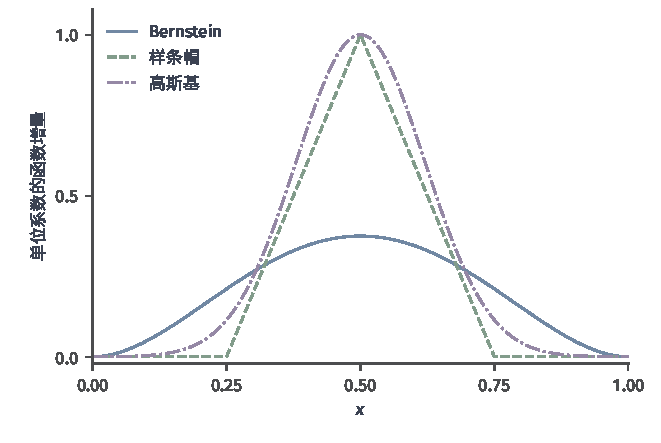
\includegraphics[width=112mm]{figures/01-mathematical-preliminaries-upper/02-linear-algebra-and-geometry/matplotlib/teaching-analysis/functional-basis-locality.pdf}
 \functionalinlinefigurecaption{fig:functional-basis-locality}
   {同一结点$1/2$处取单位系数的三类生成单元。Bernstein权重（实线）在整个$(0,1)$上非零，峰值远小于$1$；线性样条帽形函数（虚线）只在相邻两段$[1/4,3/4]$上非零，即局部支撑；高斯核截面（点划线）光滑衰减但处处非零。改变一个内部结点值只影响帽形基所在两段插值，这种局部性来自生成函数的支撑，与插值误差的凸组合界依据不同；全局基的系数依赖范围也随之更宽。}
\end{minipage}
\end{center}

\subsubsection{固定宽度高斯核截面的逼近}
\label{subsubsec:gaussian-section-approximation}

现在保持每个生成单元的宽度不变，只允许中心、线性系数和项数变化。要证明这套单元也能逼近连续目标，需要把核截面的有限和与前面的多项式逼近联系起来；证明中借助多项式，但所得近似器仍是高斯核截面的有限和。

\paragraph{固定宽度的核截面与中心差分}

在$[0,1]$固定$\sigma>0$，取
\[
  K_\sigma(x,c)=\exp\left(-\frac{(x-c)^2}{2\sigma^2}\right),
\]
并允许所有中心$c\in[0,1]$。候选近似器为
\[
  \sum_{\ell=1}^{M}a_\ell K_\sigma(\cdot,c_\ell),
\]
其中$M$和实系数可以变化；这里的稠密性采用一致范数，不对系数大小或核空间范数预设统一预算。

固定内部中心$c_0=1/2$，令$w(x)=K_\sigma(x,c_0)$。对中心连续求导：一阶导数为$\partial_cK_\sigma(x,c)=(x-c)K_\sigma(x,c)/\sigma^2$，它仍含因子$w(x)$；逐次求导便归纳地得到
\begin{equation}
  \partial_c^jK_\sigma(x,c_0)=w(x)P_j(x),
  \label{eq:functional-gaussian-derivative-polynomial}
\end{equation}
其中$P_j$是次数$j$的多项式，最高次项系数为$\sigma^{-2j}$。归纳步骤是：对$w(x)P_j(x)$再关于$c$求一次导，新增项$(x-c)wP_j/\sigma^2$只把最高次数提高一次，且首项系数乘$\sigma^{-2}$。

对每个固定$j$，取足够小的$h>0$，使$c_0,c_0+h,\ldots,c_0+jh$都在合法中心域内，写中心$j$阶前向差分
\begin{equation}
  h^{-j}\sum_{\ell=0}^{j}(-1)^{j-\ell}\binom j\ell
  K_\sigma(x,c_0+\ell h).
  \label{eq:functional-center-forward-difference}
\end{equation}
这是$j$个核截面的有限线性组合。由$\partial_c^jK_\sigma$在紧矩形$[0,1]\times[c_0-\varepsilon,c_0+j\varepsilon]$上连续，有限差分对全部$x$一致收敛到导数~\eqref{eq:functional-gaussian-derivative-polynomial}。因此每个$wP_j$都属于核截面有限和的一致闭包；不能只从逐点求导就直接宣称一致逼近，一致性来自差分在$x$上的一致收敛。

\paragraph{从加权多项式到一致稠密性}

\begin{theorem}[固定宽度高斯核截面的一致稠密性]
设$\sigma>0$固定，则全体有限和$\sum_{\ell=1}^{M}a_\ell K_\sigma(\cdot,c_\ell)$（$M$、$a_\ell$、$c_\ell$均可随目标变化）在$C([0,1])$的一致范数下稠密。
\end{theorem}

\begin{proof}
分三步。

第一步，把多项式方向并入闭包。$P_j$的最高次项非零（系数$\sigma^{-2j}\ne0$），故$P_0,P_1,\ldots,P_m$与单项式$1,x,\ldots,x^m$之间的系数变换是对角元非零的上三角变换。逐次消去最高次数，就能把任意次数至多$m$的多项式$P$写成$P_0,\ldots,P_m$的有限线性组合。于是每个加权多项式$wP$也属于核截面有限和的一致闭包。

第二步，把目标折成加权多项式。$w$在紧区间$[0,1]$上连续且严格为正，故有正下界；$f$连续时$f/w$仍连续。对$f/w$用已证明的Bernstein--Weierstrass定理，可找多项式$P$使$\|f/w-P\|_\infty$任意小，即$\|f-wP\|_\infty$任意小。

第三步，把$wP$换成真正的有限核和。把$P=\sum_j c_jP_j$写成有限组合；对每个固定$j$，由中心差分~\eqref{eq:functional-center-forward-difference}选足够小的步长，使该$wP_j$的一致逼近误差任意小。最后用三角不等式合并“$f$到$wP$”与“$wP$到有限核和”两类误差，便得到一个项数有限的高斯核截面和，其一致误差小于任意给定精度。
\end{proof}

项数和中心可以随目标及精度变化，是上述结论的条件。若只允许一个预先固定的有限中心集合，所得有限维张成在$C([0,1])$中是闭的且不等于整个空间，便不具有这种稠密性；差分中的小步长还可能带来大系数，证明不提供统一的规模、数值稳定或寻参保证。固定宽度高斯核在紧集上的通用性可与Steinwart的原论文核对\scite{steinwart2001kernel}；这里展开的是一维区间上的具体证明路线。

\subsubsection{神经网络逼近}
\label{subsubsec:neural-network-approximation}

神经单元把输入的仿射变换送入激活函数，再由有限线性组合形成输出。先对共同折点目标直接计算，再区分这个小构造与“对所有连续目标”的存在定理。

\paragraph{折点函数的两单元表示}

\begin{example}[折点函数的两ReLU表示]
定义$\operatorname{ReLU}(s)=\max(s,0)$。对$f_*(x)=|x-1/2|$，直接写
\[
  \operatorname{ReLU}\!\left(x-\frac12\right)
  +\operatorname{ReLU}\!\left(\frac12-x\right).
\]
当$x\ge1/2$时第一项为$x-1/2$、第二项为零；当$x\le1/2$时第一项为零、第二项为$1/2-x$；两端合并恰为$|x-1/2|$。分两侧核对后可见：两个输入权重取正负号、偏置都放在折点$1/2$、输出相加，各自的作用都不可省略。
\end{example}

这个单隐藏层构造使用两个ReLU单元，不要求训练过程就能验证其表示。它与线性样条共用同一折点目标是为了比较生成规则；一个简单函数有小网络，并不推出任意目标都有同样规模，也不由两侧计算推出通用逼近定理。

\paragraph{通用逼近的条件与边界}

\begin{theorem}[单隐藏层通用逼近]
固定非空紧集$X\subset\mathbb R^d$、$f\in C(X)$和连续且不是多项式的激活函数$\sigma$。采用含偏置的单隐藏层形式
\begin{equation}
  c+\sum_{j=1}^{M}a_j\sigma(w_j^{\top}x+b_j).
  \label{eq:functional-universal-approximation}
\end{equation}
则对每个$\varepsilon>0$，可以选择有限的$M$与实参数$c,a_j,w_j,b_j$，使式~\eqref{eq:functional-universal-approximation}在$X$上与$f$的一致误差小于$\varepsilon$。
\end{theorem}

这一连续激活版本由Leshno等人的结果支持\scite{leshno1993approximation}；这里陈述的是存在定理，不伪装成已经给出针对一般目标的构造算法。

用Sigmoid、Tanh和ReLU核对“连续且非多项式”的条件，可知定理不要求激活处处可微。反之，若激活是固定次数$r$的多项式，同一单隐藏层形式无论增加多少单元：仿射变换$w_j^\top x+b_j$代入$r$次多项式后仍是次数至多$r$的多项式，有限线性组合后输出次数仍至多$r$。这种固定次数空间不能在有非空内部的紧域上逼近所有连续目标（例如$x^{r+1}$在一个小区间上的行为）。因此“用了非线性”不足以替代非多项式条件，偏置也属于这里采用的定理形式。

一致误差控制全部输入位置；转为$L^2(\mu)$误差时，还要给出测度及有限总质量，才能使用
\[
  \|f-g\|_2=\left(\int_X|f-g|^2\,\mathrm d\mu\right)^{1/2}
  \le\mu(X)^{1/2}\|f-g\|_\infty.
\]
反向可能受小区域尖峰阻碍：$L^2$小而一致误差大的函数对是存在的。由评价对象不同可以说明两个逼近命题的联系与边界，同时保留这些限制：通用逼近不保证最小宽度、参数可由有限读数识别、训练收敛或泛化。

\subsection{多变量函数的组合}
\label{subsubsec:multivariable-composition}

输入分为$p,q$两组后，可以把单组函数组合成有限乘积和
\[
  F_r(p,q)=\sum_{j=1}^{r}u_j(p)v_j(q);
\]
多项式、样条或神经单元都可作为因子的构造方式。这里研究的是变量如何共同作用，改变了上一分支中“只选生成单元”的问题；项数$r$与因子幅度仍须分别记录。

下面按实际任务区分：已给整个目标函数时，构造分离近似并控制全域误差；已给规则网格读数时，构造符合这些读数的\term{张量积插值}。两者不是互斥的结构类型，网格系数也可以具有低秩；“没有指定网格读数”不是低秩的定义。先确定共同乘积结构，再说明各任务额外固定的数据和评价条件。

\subsubsection{给定函数的分离近似}
\label{subsubsec:separated-approximation}

固定整个二维目标后，问少量单组因子的乘积之和能否在整个定义域上控制误差。所构造的项数给出一个可行表示规模，不自动给出所有同规模表示中的最优误差。

\paragraph{指数函数的分离构造}

固定$E(p,q)=e^{pq}$及$(p,q)\in[-1,1]^2$，取
\begin{equation}
  E_r(p,q)=\sum_{k=0}^{r-1}\frac{p^kq^k}{k!}.
  \label{eq:functional-separated-taylor}
\end{equation}
逐项写成只依赖$p$的$p^k/k!$与只依赖$q$的$q^k$的乘积；这个Taylor构造因此使用至多$r$个分离项，不能只因它写成一个二维多项式，就跳过变量分组的识别。

因$|pq|\le1$，把$pq$看作一元变量$t$，一元指数Taylor余项给出
\[
  |e^{pq}-E_r(p,q)|\le\frac{e^{|pq|}|pq|^r}{r!}\le\frac{e}{r!}.
\]
对整个正方形取上确界后仍有相同上界，故增加项数给出一致逼近；这是一条可行截断序列的保证，并未证明它在所有$r$项分离表示中最优。

再固定$q=1$观察$r=1,2,4$：对应截面分别为$1$、$1+p$、$1+p+p^2/2+p^3/6$，在$p=1$处的误差可直接核对为$e-1$、$e-2$和$e-8/3$（即$e-8/3\approx0.052$）。这些截面与具体点值帮助解释展开过程，整个定义域上的保证仍由上一段余项估计给出。图~\ref{fig:vol1-add-functional-separated-taylor-remainder}沿$q=1$截面展示余项，不要求读者另看图片才理解界。

\begin{figure}[!htb]
  \centering
  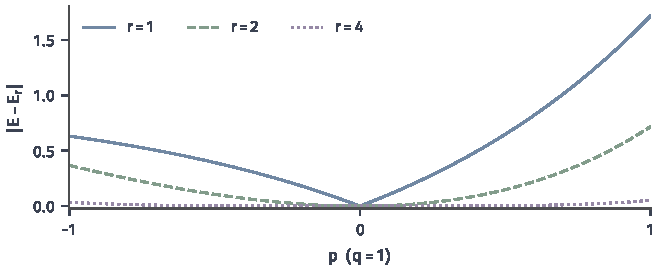
\includegraphics[width=112mm]{figures/01-mathematical-preliminaries-upper/02-linear-algebra-and-geometry/matplotlib/comprehension-additions/functional-separated-taylor-remainder.pdf}
  \caption{分离表示的截断余项。目标为$E(p,q)=e^{pq}$，$E_r$保留$k=0,\ldots,r-1$共$r$项，图中固定$q=1$并比较$r=1,2,4$的绝对误差$|E-E_r|$；三条曲线在$p=0$处均为零，随$|p|$增大而上升，$r$越大误差越小。所有曲线由解析式计算。正文界$e/r!$对整个$[-1,1]^2$成立；这里没有声称Taylor截断是最佳秩$r$逼近。}
  \label{fig:vol1-add-functional-separated-taylor-remainder}
\end{figure}

\paragraph{分离项的尺度与适用范围}

把$r$个因子分别组成向量$u(p)$与$v(q)$，其第$j$个分量为$u_j(p)$与$v_j(q)$，由Cauchy--Schwarz得
\[
  |F_r(p,q)|=\left|\sum_{j=1}^ru_j(p)v_j(q)\right|
  \le\|u(p)\|_2\|v(q)\|_2.
\]
项数说明表示用了多少个分离方向，因子范数控制这些方向的幅度；相同项数并不限制输出大小，也不独自控制函数类在指定误差下的覆盖数。某些Bellman残差矩阵也使用两个因子内积的形式，可据此辨认结构上的类比；但矩阵条目的含义、可实现性、查询协议与样本结论都依赖相应决策任务。这里不从$e^{pq}$的Taylor误差或一般因子界推出强化学习保证，函数类的统一代表数量留给覆盖数任务另行定义。

\subsubsection{网格数据的张量积插值}
\label{subsubsec:tensor-grid-interpolation}

现在不预先给出整个目标，只固定单位整数网格上的样本值$U_{ij}$，希望在非整数位置求值且经过原有网格读数。共同形式是
\begin{equation}
  S(x,y)=\sum_{i,j}c_{ij}h(x-i)h(y-j);
  \label{eq:functional-tensor-interpolation}
\end{equation}
一维核决定每轴的衔接与支撑，系数如何由样本产生则是另一项必须核对的条件。有限网格须指定边界延拓；下面B样条的可逆论证明确采用周期边界，不能自动移给其他端点条件。

三种方案在同一任务下比较结点插值、导数连续、取值范围和计算依赖：双线性和三次卷积可以直接用样本作系数；三次B样条则要先恢复系数再局部求值。这个差别在选择局部核时就必须注意，不能以“都具有有限支撑”掩盖样本到系数的过程。

\paragraph{双线性插值}

定义帽核$h(s)=\max(1-|s|,0)$，核对$h(0)=1$、非零整数处为零（基数条件）。取$c_{ij}=U_{ij}$时，整数网格位置$(i,j)$只留下对应的一个样本$U_{ij}$，因此满足插值；二维形式由两轴核的乘积生成。

对查询$(x,y)=(i+s,j+t)$、$s,t\in[0,1]$，只有四个核同时非零，展开权重
\[
  (1-s)(1-t),\quad s(1-t),\quad (1-s)t,\quad st
\]
及其对应四角样本$U_{i,j},U_{i+1,j},U_{i,j+1},U_{i+1,j+1}$。每项非负且总和为一，所以输出落在这四个样本的最小值和最大值之间；范围保持来自凸组合，而非来自“线性”这个名称。固定一个坐标时输出关于另一坐标线性；共同展开一般含$st$交叉项，所以通常不是整个平面上的仿射函数。相邻单元在公共边使用同一线性插值，函数值能够衔接，一阶导数一般会跳变；这也明确了更换核所要改善的是哪一种连续性。给定边界延拓后，每次求值只用所在单元四角样本，也可先沿一轴再沿另一轴计算。

\paragraph{三次卷积插值}

令$r=|s|$，定义Keys核：
\[
  h_a(s)=
  \begin{cases}
    (a+2)r^3-(a+3)r^2+1,&0\le r\le1,\\
    ar^3-5ar^2+8ar-4a,&1<r<2,\\
    0,&r\ge2.
  \end{cases}
\]
先检查衔接：$r=1$处左段值$(a+2)-(a+3)+1=0$、右段值$a-5a+8a-4a=0$，两侧一阶导数分别为$3(a+2)-2(a+3)=a$与$3a-10a+8a=a$，故函数值与一阶导数都连续；$r=2$处右段值$8a-20a+16a-4a=0$、导数$12a-20a+8a=0$，与外侧零相接；原点处两段关于$|s|$对称。综合得到$C^1$衔接和有限支撑$[-2,2]$；整数处的基数条件使样本仍能直接作系数。

对单位单元内位置$s\in[0,1]$，四个非零结点$-1,0,1,2$的权重为
\[
  h_a(s+1),\ h_a(s),\ h_a(s-1),\ h_a(s-2).
\]
把对应分段式展开相加得到一；再将两轴权重和相乘传到二维，便取得常量保持。这个计算不要求各权重非负，因此尚不能推出样本范围保持。

\begin{example}[半格查询的过冲]
取$a=-1/2$、查询半格$s=1/2$。由核的对称分段式算得四权重
\[
  \frac{(-1,\,9,\,9,\,-1)}{16}.
\]
若相应四个样本取$0,0,0,16$，则输出为$(-1\cdot0+9\cdot0+9\cdot0-1\cdot16)/16=-1$，越出样本区间$[0,16]$。这个直接可算的例子说明：$C^1$衔接与常量保持可以成立，同时仍发生过冲；二维张量积也不能仅靠提高衔接阶数取得范围保证。
\end{example}

二维每次求值至多使用$4\times4$个样本，此时系数就是样本，有限支撑确实对应直接样本的局部计算。这里不陈述未经额外光滑性和边界条件核对的全域误差阶。

\paragraph{三次B样条的系数恢复与求值}

定义中心\term{三次B样条}，令$r=|s|$：
\[
  \beta_3(s)=
  \begin{cases}
    \frac23-r^2+\frac12r^3,&0\le r<1,\\
    \frac16(2-r)^3,&1\le r<2,\\
    0,&r\ge2.
  \end{cases}
\]
核对分段处$r=1$的函数值（左段$2/3-1+1/2=1/6$，右段$(2-1)^3/6=1/6$）及一、二阶导数，均取得连续，故$\beta_3\in C^2$；再算
\[
  \beta_3(0)=\frac23,\qquad \beta_3(\pm1)=\frac16,\qquad \beta_3(\pm2)=0.
\]
这些整数值不满足直接用样本作系数所需的基数条件（$\beta_3(0)\ne1$、$\beta_3(1)\ne0$）。

先在一维写
\[
  S(x)=\sum_jc_j\beta_3(x-j),
\]
在整数结点代入得到
\begin{equation}
  S(i)=\frac{c_{i-1}+4c_i+c_{i+1}}6.
  \label{eq:functional-cubic-bspline-prefilter}
\end{equation}
若要求$S(i)=U_i$，必须先解这个“样本到系数”的线性系统；直接设$c_i=U_i$得到的是邻近样本的平滑累计，通常不会经过原样本。这样先看清不插值的原因，也就明白为什么需要系数恢复。

对长度$N$的周期网格，把下标按模$N$解释，并将周期正弦、余弦方向$c_j=e^{i\omega j}$代入上述卷积。频率$\omega=2\pi k/N$的响应为
\[
  \frac{e^{-i\omega}+4+e^{i\omega}}6=\frac{4+2\cos\omega}{6}\ge\frac{4-2}{6}=\frac13,
\]
所以所有周期方向上的响应非零，可唯一恢复系数；这一步也称预滤波。若改用其他边界规则，要先写出其端点方程再检查相应系统，不能沿用这个周期响应证明。二维样本到系数的关系是两个一维卷积沿两轴相继作用，因此先沿一轴恢复系数、再沿另一轴恢复，最后在查询点用张量积局部核求值。每个查询只访问邻近系数，但预滤波可能让一个原样本影响远处系数；因此“局部求值”与“结果只依赖邻近原样本”必须分别判断。

在单位单元内把四个非零B样条核权展开相加得到一；核权非负及其和为一至多把输出限制在“有关系数”的范围内，而系数已经过恢复，未必落在原样本取值范围，不能据此宣称原样本范围保持。回看三套方案，结点插值、$C^0/C^1/C^2$衔接、取值范围及计算依赖各有自己的核验依据。若后续缩小采样网格，还要按新的采样问题处理混叠；提高插值核阶数本身并不完成抗混叠。

\section{连续能量的离散逼近}
\label{sec:discrete-energy-approximation}

这里固定一个已知函数或一组函数记录，把连续积分目标改写成有限累计，研究权重、尺度和采样是否仍表达原来的量。它与“选择一个表示函数”不同，也与“重新求一个离散最优函数”不同；因此单独讨论能量值的逼近及扰动，不把这些结论并入拟合解稳定性。

本节按采样几何分为规则网格和一般点云；每种几何内部核对差分、积分权重与适用条件。点云分支在定义离散二次型后，还固定记录并核对边权变化怎样影响能量值，使扰动估计紧接其实际目标。

\subsection{规则网格的能量权重}
\label{subsubsec:regular-grid-energy}

\paragraph{从导数与积分尺度得到离散能量}

在$[0,1]$取
\[
  x_i=ih,\qquad i=0,\ldots,n,\qquad h=\frac1n,
\]
固定$f\in C^1([0,1])$。当前目标是
\[
  \frac12\int_0^1|f'|^2,
\]
网格值都来自同一个已知$f$，没有把节点值改成待求未知量。

邻点差先除以$h$才形成导数近似，平方后还要乘上积分单元长度$h$，所以定义
\begin{equation}
  E_h(f)=\frac1{2h}\sum_{i=0}^{n-1}\bigl[f(x_{i+1})-f(x_i)\bigr]^2.
  \label{eq:functional-grid-energy}
\end{equation}
要分别说明差商中的$h^{-2}$与积分中的$h$：单个差商$[f(x_{i+1})-f(x_i)]/h$近似导数，其平方乘单元长度$h$才是一个单元上的能量微元；合起来因子$1/(2h)$使最终权重的来源可复核，而不是把未归一化的邻差平方误当成同一能量。

\paragraph{已知函数的能量一致性}

\begin{theorem}[$E_h$的连续极限]
若$f\in C^1([0,1])$，则当$h\to0$时
\begin{equation}
  E_h(f)\to\frac12\int_0^1|f'(x)|^2\,\mathrm dx.
  \label{eq:functional-grid-energy-convergence}
\end{equation}
\end{theorem}

\begin{proof}
把差商写成局部导数平均：
\[
  \frac{f(x_{i+1})-f(x_i)}h=\frac1h\int_{x_i}^{x_{i+1}}f'(s)\,\mathrm ds.
\]
$f'$在紧区间上一致连续，故对单元内任意点$x_i+\theta h$，平均值与该点导数值之差不超过$\omega_{f'}(h)$；特别地，它与$|f'|^2$在单元上的代表值之差，在$f'$有界时被$\omega_{f'}(h)$与$\|f'\|_\infty$的乘积控制。于是
\[
  E_h(f)=\frac12\sum_{i=0}^{n-1}h\left(\frac{f(x_{i+1})-f(x_i)}h\right)^2
\]
与Riemann和$\frac12\sum_i h|f'(x_i)|^2$之差随$h\to0$趋于零；而$|f'|^2$连续，该Riemann和趋于$\frac12\int_0^1|f'|^2$。这里先处理同一函数的导数近似，再累计积分，两个步骤各有所需条件，不能只凭“网格变密”宣布极限。
\end{proof}

这个结论没有重新求最小者，因此不证明离散解逼近连续解。未知网格值的五点系统、固定边界唯一性以及足够光滑条件下的差分一致性，由后续微分方程章的五点差分处理；能量值一致、系统可解和解收敛必须分别建立。

\subsection{点云的能量权重与归一化}
\label{subsubsec:point-cloud-energy}

\paragraph{对称边权与点对计数}

给定固定标量记录$f_i$及对称非负边权
\[
  w_{ij}=w_{ji}\ge0,
\]
约定
\begin{equation}
  E_n(f)=\frac12\sum_{i,j=1}^nw_{ij}(f_i-f_j)^2
  \label{eq:functional-point-cloud-energy}
\end{equation}
遍历有序点对。非负性保证代价非负，对称性允许用无向边解释；对角项为零，每条非自环无向边则计了两次。

保持同一权重时，由对称性
\[
  E_n(f)=\sum_{i<j}w_{ij}(f_i-f_j)^2;
\]
若无向边“一次”的公式还带$1/2$，其有序和就应带$1/4$，或相应改变权重定义。要先核对求和对象，再比较系数和归一化，不能只凭表面的$1/2$判断两个目标相同或不同。

\paragraph{离散累计何时具有连续解释}

规则网格曾提供单元长度和邻点距离，点云却没有自动给出这些量。若要把式~\eqref{eq:functional-point-cloud-energy}解释为连续梯度能量的近似，必须另给采样密度、邻近半径、核权、样本规模的归一化以及目标函数的正则性，并说明它们怎样把局部差平方变成积分。

条件没有给全时，只能把$E_n$视为一个合法的离散二次目标，不宣称任意图能量都收敛到某个连续几何能量。当前标量记录能够直接相减；若记录为不同点的切向量，还必须规定跨点比较或搬运，相关联络条件由流形章建立。

\paragraph{离散能量值的扰动界}

固定$f_i$、有序点对与前面的系数约定，把权重改为$\widetilde w_{ij}$，记
\[
  \delta w_{ij}=\widetilde w_{ij}-w_{ij}.
\]
直接相减两个目标、逐项取绝对值，得到
\begin{equation}
  |\widetilde E_n(f)-E_n(f)|
  \le\frac12\sum_{i,j=1}^n|\delta w_{ij}|(f_i-f_j)^2.
  \label{eq:functional-energy-weight-perturbation}
\end{equation}
若新旧目标都要求非负能量，还应各自核对边权非负。右端同时取决于权重差和当前记录的邻点差，不能只看边权变了多少而忽略所评价的函数。这个上界控制的是同一记录的目标值，既没有重新最小化，也没有比较两个最优函数，因此不能当成解稳定定理。

\paragraph{目标权重与计算内积的区别}

若这些边权进入目标二次型，改变权重就改变了最优化问题；若目标保持不变，只改变用于表示微分的内积，则目标最优者不因此改变，梯度和演化方向却会改变。可以回用前面的仿射梯度例，明确“改权重”发生在哪个数学对象上。非负性只说明目标下界，不能替代扰动界、最小值达到或算法收敛。由此把本节能量值的稳定性与前面的有界运算、数据到最优函数的稳定性区分开，离散目标的条件留在其实际使用位置。

\section{函数类的覆盖数}
\label{sec:covering-numbers}

此前是为一个给定目标构造近似函数，或为一个拟合任务求解。这里改为固定整个非空函数类，问预先准备多少代表才能近似其中每个成员。这需要共同给定类、误差口径、精度和代表范围；单个目标可逼近、参数个数有限或谱有效维度有限，都不能直接代替这个问题。

本节按评价输入是否预先固定，分为普通覆盖与依历史变化的查询树覆盖。它们改变的是评价协议和代表对象，不能仅按阅读先后把后者说成前者的同一距离。

\subsection{固定距离下的覆盖数}
\label{subsubsec:covering-number-fixed}

\paragraph{距离、代表集合与量词}

\begin{definition}[固定距离下的覆盖数]
固定非空类$\mathcal F$、距离或伪距离$d$和精度$\delta>0$，先约定代表属于$\mathcal F$。有限集$V\subseteq\mathcal F$若对所有$f\in\mathcal F$都存在$v\in V$使
\[
  d(f,v)\le\delta,
\]
就构成一个$\delta$-覆盖；用最少代表数定义
\begin{equation}
  N(\delta,\mathcal F,d),
  \label{eq:functional-covering-number}
\end{equation}
无有限覆盖时记为无穷。若允许类外中心，必须另行说明该约定，不能无声改变数值口径。
\end{definition}

代表集必须在选定待近似成员之前固定，并覆盖所有成员；平均只对某些函数近似良好不能满足要求。全域上确界、指定测度的$L^2$误差和固定样本上的均方根是不同口径；经验误差可能为零而域外函数不同，因此通常只是伪距离。

覆盖数中的最坏要求针对类中每个函数，量词是“存在一个有限代表集，对所有函数存在近邻”：
\[
  \exists\,V\subset\mathcal F,\ \text{有限}\quad\text{s.t.}\quad
  \forall f\in\mathcal F,\ \exists v\in V:\ d(f,v)\le\delta.
\]
具体代表可以随函数选择，代表集则共同固定；先把允许集合与误差说清，再谈代表最少多少。图~\ref{fig:functional-covering-centers}在一个系数平面上展示覆盖的几何图景，正文随后对一个一维常值族给出显式估计。

\begin{center}
\begin{minipage}{\linewidth}
 \centering
 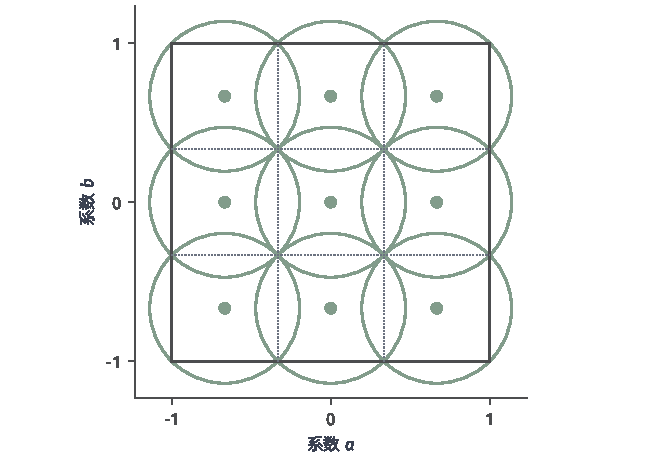
\includegraphics[width=112mm]{figures/01-mathematical-preliminaries-upper/02-linear-algebra-and-geometry/matplotlib/concepts-analysis-functional/covering-centers.pdf}
 \functionalinlinefigurecaption{fig:functional-covering-centers}
   {覆盖一个区域的几何图景。方形区域$[-1,1]^2$上，$9$个半径$\sqrt2/3$的圆盘中心排成$3\times3$网格$\{-2/3,0,2/3\}^2$；方形四角到最近中心的距离恰为$\sqrt2/3$，故整个方形被覆盖。代表数由区域在所选度量下的延伸和精度决定；正文对一维常值族给出显式估计$N\ge M/(2\delta)$。参数个数未变，区域尺度变大却使所需代表数增大。}
\end{minipage}
\end{center}

图~\ref{fig:functional-covering-centers}的系数平面并非抽象网格：它对应一元仿射函数类
\[
  f(t)=a+bt,\qquad (a,b)\in[-1,1]^2,\quad t\in[-1,1].
\]
两条仿射函数之差为$(a-a')+(b-b')t$，在上确界范数下的最大值在端点$t=\pm1$取得，等于$|a-a'|+|b-b'|$，即系数平面上的$\ell^1$距离（图中画欧氏圆盘只是几何示意；$\ell^1$球实为菱形）。把方形区域按精度$\delta$分块时，两个方向各需约$1/\delta$个中心，代表总数按$\delta^{-2}$增长；这与下一段一维常值族$N\ge M/(2\delta)$形成对照——代表数不仅随输出尺度$M$增大，还随参数维数与区域延伸增大。评价的始终是函数类在所选范数下的实际大小，而不是参数个数。

\paragraph{尺度与类的大小}

在非空输入域上取常值族
\[
  f_\theta(x)=M\theta,\qquad \theta\in[0,1],\quad M>0,
\]
使用上确界距离。一个代表常值函数$v$在半径$\delta$内所能覆盖的取值区间长度为$2\delta$（即$[v-\delta,v+\delta]$），而整个类的取值扫过$[0,M]$；要覆盖这个长度必须$N\cdot2\delta\ge M$，故
\[
  N(\delta,\mathcal F,d_\infty)\ge\frac{M}{2\delta}.
\]
参数数目没有变，输出尺度$M$却能使所需代表数增大。

对另一个常值族
\[
  f_\theta(x)=\sin(M\theta),\qquad \theta\in[0,2\pi],
\]
$M$为正整数，输出始终覆盖相同的$[-1,1]$，所以函数类本身没有随$M$扩大。参数导数可以变大，却不单独决定函数集合和覆盖数；这个对照说明应评价实际类，而不是只数参数或看参数化速度。

前面的折点目标可用多项式、样条或ReLU表示，回答的是单个函数的预算。若改问一整个类，就必须另外指定其范数半径、导数条件或其他约束，再在同一距离和精度下计算覆盖；不能由单例的精确表示取得全类的统一结论。

\paragraph{覆盖数与其他容量量的边界}

在后续学习理论中还会遇到两个容量量：伪维是在固定输入与阈值下检查哪些跨阈值模式可实现，胖打散还要求阈值两侧有指定间隔；覆盖数则累计给定距离下的近似代表数量。三者的评价对象与精度条件各不相同，不能从名称相近直接互换。谱有效维度依赖算子与惩罚尺度（见本章正则化参数极限一节），覆盖数依赖实际函数类及其距离；两者可以在额外定理下联系，却都不独自保证统计误差小、可识别或优化可解。相应学习结论留到后续学习理论中建立。

\subsection{查询树上的序贯覆盖数}
\label{subsubsec:sequential-covering}

\paragraph{从固定输入向量到查询树}

固定深度$T\ge1$的\term{查询树}
\[
  x_t:\{-1,1\}^{t-1}\to X,
\]
用$\sigma\in\{-1,1\}^{T}$表示一条分支路径。当前查询只依赖已有分支$\sigma_{<t}$，所以一个函数$f$在树上产生
\[
  f(x_t(\sigma_{<t}));
\]
这个对象有多个可能路径，不是一条预先固定的样本向量。

相应代表为实数树
\[
  v_t:\{-1,1\}^{t-1}\to\mathbb R.
\]
先固定一个有限树集合$\mathcal V$，再要求对每个$f\in\mathcal F$和每条$\sigma$，存在$v\in\mathcal V$使
\begin{equation}
  \left(\frac1T\sum_{t=1}^{T}
  \left|f(x_t(\sigma_{<t}))-v_t(\sigma_{<t})\right|^2\right)^{1/2}
  \le\delta.
  \label{eq:functional-sequential-cover}
\end{equation}
均方根只沿当前路径累计，代表树不必来自$\mathcal F$中的一个普通函数。

\paragraph{路径量词与最坏查询协议}

单独展开量词
\[
  \forall f\in\mathcal F\ \forall\sigma\in\{-1,1\}^T\ \exists v\in\mathcal V:
\]
有限树集合$\mathcal V$预先固定，所选代表树可随函数和路径改变。若改成“每个$f$先选一个代表并同时匹配所有路径”，就是更强的要求，不能把两种定义混用。

在给定查询树上取最小代表树数量，再对全部允许的深度$T$查询树取上确界，定义
\begin{equation}
  N_2^{\mathrm{seq}}(\delta,\mathcal F,T).
  \label{eq:functional-sequential-cover-number}
\end{equation}
这个上确界比较的是最坏查询协议，不是在路径上取随机平均；固定路径误差与“全部查询树最坏情形”是两个连续的定义步骤。例如两层树的根查询固定为$x_0$，第一次结果$\epsilon_1=-1$或$+1$后，第二次查询分别取$x_-$与$x_+$；代表树也要相应给出根处的$v_1$和两个第二层数值$v_2(-1)$、$v_2(+1)$。图~\ref{fig:functional-query-tree}用这个最小例子说明为什么不能用单个固定的两维样本向量替代树。这个定义只给组合容量，学习或预测保证另需具体任务和相应定理。

\begin{center}
\begin{minipage}{\linewidth}
 \centering
 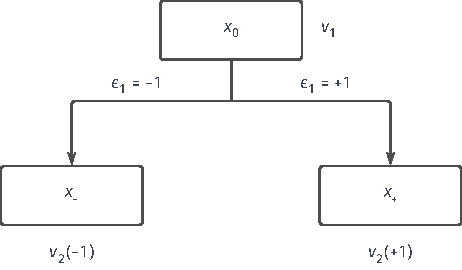
\includegraphics[width=78.281mm]{figures/01-mathematical-preliminaries-upper/02-linear-algebra-and-geometry/tikz/concepts-analysis-functional/query-tree.pdf}
 \functionalinlinefigurecaption{fig:functional-query-tree}
   {两层查询树。根查询$x_0$固定；第一次结果$\epsilon_1=-1$进入左支，第二次查询取$x_-$，结果$\epsilon_1=+1$进入右支，第二次查询取$x_+$。代表树在根处给$v_1$，在两个第二层结点分别给$v_2(-1)$与$v_2(+1)$。评价沿每条分支路径累计均方根误差，因此它不是一个固定两维样本向量，而是随历史变化的查询协议。}
\end{minipage}
\end{center}

\section{本章小结}
\label{sec:functional-summary}

\begin{enumerate}
  \item 把整个函数当作空间元素，必须先明确它是逐点函数还是几乎处处等价类，再选择误差、线性运算和完备性条件。Banach、Hilbert、$L^p$与核空间分别规定不同结构，不能当成彼此排斥的类别；同一底集或相同函数集合也不意味着误差口径相同。

  \item 弱导数通过测试恒等式保留变化信息，Sobolev范数同时控制函数与规定阶导数；它们不自动提供每点或边界读数。读取首先要良定义，随后才判断有界、代表唯一及位置变化；Riesz表示、RKHS和迹各有明确的输入、输出和条件。

  \item 正交展开、积分变换和积分方程分别记录方向、改变函数以及确定未知函数。闭性与完备性保障投影，正交系稠密保障范数展开，紧自伴和Mercer条件保障不同层次的谱结论；压缩迭代还要核对实际自映射和严格常数，不能只凭一个形式核公式取得全部结论。

  \item 函数拟合必须把数据、候选、目标和允许扰动同时给清。表示定理消去数据看不见的方向，具体二次结构才进一步给出有限系统和唯一函数；系数冗余、算法收敛、固定参数的数据稳定以及惩罚参数极限仍按各自变化量判断。积分变分先得到一阶弱条件，具体Poisson与热方程的解理论由后续微分方程章承接。

  \item 有限表示构造、已知函数的能量采样与整个函数类的覆盖数具有不同的近似对象。一个目标存在逼近器不保证找得到参数，能量值一致不保证最优解收敛，容量数量也不直接保证泛化；每一种判断都必须保留其误差、量词和条件。曲面弱微分（\term{Laplace--Beltrami算子}）、球面谱（\term{球谐函数}）、多尺度平滑（\term{尺度空间}）以及跨点搬运所需的几何结构，由流形章继续建立。
\end{enumerate}

